% File:   TsuiteDE_UserGuide.tex
% Author: Mariarosaria Rizzardi


\documentclass[a4paper,10pt]{report}%{book}
%\documentclass[a4paper,twoside,10pt]{article}
% Alternative Options: %%%%%%%%%%%%%%%%%%%%%%%%%%%%%%%%%%%%%%%%%%%%%%%%%
%   Paper Size: a4paper / a5paper / b5paper / letterpaper / legalpaper / executivepaper
%   Duplex: oneside / twoside
%   Base Font Size: 10pt / 11pt / 12pt

%\usepackage{blindtext}

%% Language %%%%%%%%%%%%%%%%%%%%%%%%%%%%%%%%%%%%%%%%%%%%%%%%%
%\usepackage[UKenglish,italian]{babel}
%\usepackage[latin1]{inputenc} % per le vocali accentate (non funziona con \usepackage[ansinew]{inputenc})
\usepackage[USenglish]{babel} %francais, polish, spanish, italian, ...
\usepackage[T1]{fontenc}
\usepackage[ansinew]{inputenc}
\usepackage{lmodern} %Type1-font for non-english texts and characters (SERVE PER PDF)

%% the bibliography will appear as a chapter in the document
\usepackage[nottoc,numbib]{tocbibind}

%% Math Packages %%%%%%%%%%%%%%%%%%%%%%%%%%%%%%%%%%%%%%%%%%%%
\usepackage{amsmath,amssymb}
\usepackage{amsthm} % per usare \begin{proof} ... \end{proof}
%\renewcommand{\qedsymbol}{\small$\blacksquare$} % quadratino nero per fine dimostrazione
\usepackage{amsfonts}

\usepackage{mathrsfs} % per \mathscr{L}: L di Laplace Transform
\usepackage{cancel}   % per cancellare simboli in formule

%\usepackage{quotes} % si puo' usare "xxx"


%% TABLES %%%%%%%%%%%%%%%%%%%%%%%%%%%%%%%%%%%%%%%%%%%%
\usepackage{siunitx} % in tabular per allineare al punto decimale
%\usepackage{longtable} % per tabelle su più pagine
%\usepackage{multirow}


%% Packages for Graphics & Figures %%%%%%%%%%%%%%%%%%%%%%%%%%
\usepackage{graphicx} %%For loading graphic files
\usepackage[usenames,dvipsnames]{xcolor} 
%\usepackage{subfig} %%Subfigures inside a figure
%\usepackage{pst-all} %%PSTricks - not useable with pdfLaTeX


\usepackage[hyphens]{url}
\usepackage[ps2pdf,breaklinks,colorlinks=true,linkcolor=cyan,citebordercolor=green,linkbordercolor=cyan]{hyperref}
%% others: if you use colorlinks=true you can set (defaults in []):
    %linkcolor [red]
    %anchorcolor [black]
    %citecolor [green]
    %filecolor [cyan]
    %menucolor [red]
    %runcolor [cyan - same as file color]
    %urlcolor [magenta]
    %allcolors -- use this if you want to set all links to the same color


%\usepackage[breaklinks,colorlinks=true]{hyperref}


%% Packages for Line numbering and Hidden text %%%%%%%%%%%%%%%%%%%%%%%%%%
%\usepackage[pagewise,mathlines]{lineno}
\usepackage{comment} % per nascondere testo

%\usepackage{algorithm2e}

%% MATLAB Style %%%%%%%%%%%%%%%%%%%%%%%%%%
%\usepackage[framed,numbered,bw]{mcode}
%\usepackage[framed,bw]{mcode}
%\usepackage[framed,bw]{My_mcode}

\usepackage{listings}
\lstset{language=C++,
        showstringspaces=false,
        basicstyle=\footnotesize\ttfamily,
        %basicstyle=\small\ttfamily,
        commentstyle=\scriptsize\ttfamily,
        %commentstyle=\footnotesize\ttfamily,
        frame=single,
        %frame=none,
        %keywordstyle=\color{black}
        }


%% Please note:
%% Images can be included using \includegraphics{Dateiname}
%% resp. using the dialog in the Insert menu.
%% 
%% The mode "LaTeX => PDF" allows the following formats:
%%   .jpg  .png  .pdf  .mps
%% 
%% The modes "LaTeX => DVI", "LaTeX => PS" und "LaTeX => PS => PDF"
%% allow the following formats:
%%   .eps  .ps  .bmp  .pict  .pntg


%% Line Spacing %%%%%%%%%%%%%%%%%%%%%%%%%%%%%%%%%%%%%%%%%%%%%
%\usepackage{setspace}
%\singlespacing        %% 1-spacing (default)
%\onehalfspacing       %% 1,5-spacing
%\doublespacing        %% 2-spacing


%% Other Packages %%%%%%%%%%%%%%%%%%%%%%%%%%%%%%%%%%%%%%%%%%%
\usepackage{a4wide} %%Smaller margins = more text per page.
%\usepackage{fancyhdr} %%Fancy headings

\usepackage{wallpaper} %%to insert a background image
\addtolength{\wpYoffset}{-7cm} %% sposta l'immagine di CenterWallPaper in basso di  8 cm dal centro
%\addtolength{\wpYoffset}{10cm} %% sposta l'immagine di CenterWallPaper in alto di 11 cm dal centro



%%%%%%%%%%%%%%%%%%%%%%%%%%%%%%%%%%%%%%%%%%%%%%%%%%%%%%%%%%%%%
%% DOCUMENT
%%%%%%%%%%%%%%%%%%%%%%%%%%%%%%%%%%%%%%%%%%%%%%%%%%%%%%%%%%%%%
\begin{document}

\pagestyle{empty} %No headings for the first pages.

%% Title Page %%%%%%%%%%%%%%%%%%%%%%%%%%%%%%%%%%%%%%%%%%%%%%%
%% ==> Write your text here or include other files.

%% The simple version:
\title{{\Huge Talbot Suite DE} \\[.3in] {\Huge User Guide} \\[.6in]
       {\large March 2017} \\[.6in]}
\author{
{\Large Mariarosaria Rizzardi} \\[.3in]
{\href{mariarosaria.rizzardi@uniparthenope.it}{mariarosaria.rizzardi@uniparthenope.it}} \\[.3in]
{{\sl DiST} - Dept.~of Science and Technology} \\
{{\it Parthenope} University, Naples (Italy)} \\[2.25in]
{\small{\sl DiST} - Dipartimento di Scienze e Tecnologie} \\
{\small Universit\`a degli Studi di Napoli {\it Parthenope}} \\
{\small Centro Direzionale di Napoli, Isola C4 - 80143 Napoli (I)}
}
\date{} %% If commented, the current date is used.

%\ThisCenterWallPaper{0.12}{./FIGS/LOGOparthenope2_gray.eps}
\ThisCenterWallPaper{0.12}{./FIGS/LOGOxArticulate_100_gray1.eps}

\clearpage\maketitle
\thispagestyle{empty} %No headings for the first pages.
%%%%%%%%%%%%%%%%%%%%%%%%%%%%%%%%%%%%%%%%%%%%%%%%%%%%%%%%%%%%%


%% The nice version:
%\input{titlepage} %%You need a file 'titlepage.tex' for this.
%% ==> TeXnicCenter supplies a possible titlepage file
%% ==> with its templates (File | New from Template...).


%% Inhaltsverzeichnis %%%%%%%%%%%%%%%%%%%%%%%%%%%%%%%%%%%%%%%
%\tableofcontents %Table of contents
%\cleardoublepage %The first chapter should start on an odd page.

\newpage
\pagestyle{plain} %Now display headings: headings / fancy / ...
\pagenumbering{roman} % change to roman
%\frontmatter
\tableofcontents
%\mainmatter


\newpage
\pagenumbering{arabic} % change to arabic
\setcounter{page}{1}

%%%%%%%%%%%%%%%%%%%%%%%%%%%%%%%%%%%%%%%%%%%%%%%%%%%%%%%%%%%%%%%%%%%%%%%%%%%%%%%%%%
\chapter{FUNCTION DOCUMENTATION}\label{CHAPT1}
\setcounter{secnumdepth}{1}
%%%%%%%%%%%%%%%%%%%%%%%%%%%%%%%%%%%%%%%%%%%%%%%%%%%%%%%%%%%%%%%%%%%%%%%%%%%%%%%%%%


%%%%%%%%%%%%%%%%%%%%%%%%%%%%%%%%%%%%%%%%%%%%%%%%%%%%%%%%%%%%%%%%%%%%%%%%%%%%%%%%%%
\section{{\tt Talbot Suite DE}}\label{TSUITEDE}
%%%%%%%%%%%%%%%%%%%%%%%%%%%%%%%%%%%%%%%%%%%%%%%%%%%%%%%%%%%%%%%%%%%%%%%%%%%%%%%%%%
The Laplace Transform (LT), $F(s)$, of $f(t)$ is defined as
\[
F(s) = \mathscr{L}[f] = \int_0^\infty f(t) e^{-st} dt
\]
when this integral exists. The inverse problem is to reconstruct $f(t)$ from $F(s)$.
\\
{\em Talbot's method} \cite{Talbot:1979} is an automatic method for the numerical inversion of Laplace
Transforms, designed to invert a Laplace Transform at a single value.
It has been implemented in FORTRAN \cite{Talbot:1990}.
On the other hand, {\em modified Talbot's method} \cite{Talbot:1995} is designed for multi-point
inversion problems.
These two methods have been implemented in C \cite{TALBOT_SUITE:2014} by a parallel software designed
for parallel distributed (MPI-based) and shared (OpenMP-based) memory architectures.
Like other software for the numerical inversion of Laplace Transforms, all of them require, among their
input parameters, a user-defined function for the Laplace Transform to be inverted: for this reason they
are not suited to solve differential problems where the Laplace Transform is only known as numerical
samples.
\\
On the contrary, the algorithm in {\tt Talbot Suite DE} \cite{Talbot:2016} has been designed especially
for this kind of problems ({\tt DE} stays for Differential Equations), since it requires, as an input
parameter, a user-defined function returning the samples of the Laplace Transform computed at an input
complex array.

{\tt Talbot Suite DE} contains the sequential implementations of {\em Talbot's method} and of
{\em modified Talbot's method} and the parallel (OpenMP-based) implementations of {\em modified Talbot's
method}; it also contains the sequential version of {\tt Talbot Suite}, not provided in \cite{TALBOT_SUITE:2014}.
\\
About the OpenMP-based parallel version, two parallelization strategies have been implemented to solve
multi-point inversion problems; they are denoted as {\em coarse-grained} and {\em fine-grained
parallelism} respectively: the former distributes data among the $p$ parallel processes and computes
sequentially each summation approximating the inverse Laplace Transform, the latter parallelizes the
summation inside a sequential for-loop over the data.
The former is particularly useful when the inversion must be carried out at many values of $t$, while
the latter is useful when the final summations contain a lot of terms. In addition, a hybrid
parallelization strategy is provided: it merges together the two previous strategies. This is carried
out by means of a {\em nested parallelism} in OpenMP.
Some computing environments require that {\em nested parallelism} has to be explicitly enabled: the
provided code checks for it and, if necessary, enables the {\em nested parallelism} in OpenMP otherwise
results will be quite wrong.
Of course, the hybrid parallelization strategy is useful when the inversion must be carried out at many
values of t and the final summation contains a lot of terms. However, in many other cases (a few values
of $t$ and a few terms in the summations) it is sufficient to use the sequential version instead of the
parallel one.

The function names in {\tt Talbot Suite DE} follow the same convention as in {\tt Talbot Suite}: the
leftmost number "1" refers to the {\em modified method} and "2" to the {\em classical method}.
The prefix "{\tt SEQ}" refers to the sequential version, "{\tt OMP}" to the parallel OpenMP-based version.
All the functions in {\tt Talbot Suite DE} have the suffix {\tt DE}, while the sequential implementation
of {\tt Talbot Suite} does not.
In the OpenMP version of {\tt Talbot Suite DE}, the righmost number denotes the parallelization
strategy: "1" for {\em coarse-grained}, "2" for {\em fine-grained} and "3" for {\em hybrid parallelism}.
\\[.15in]
The general algorithm, behind the two Talbot methods, can be logically divided into two main steps:
estimation of method's parameters, and evaluation of summations that approximate the inverse Laplace
Transform values.
The software suite can be used by not expert or expert users: the former, to solve the problem, calls a
single "user-level" function; the latter calls the "skill-level" functions so that he is able to change
parameters.
\\
User-level functions are:
\begin{itemize}
\item {\tt SEQ\_Talbot1\_DE}: sequential implementation of the {\em modified method} for DE.
\item {\tt SEQ\_Talbot2\_DE}: sequential implementation of the {\em classical method} for DE.
\item {\tt SEQ\_Talbot1}: sequential implementation of the {\em modified method}.
\item {\tt SEQ\_Talbot2}: sequential implementation of the {\em classical method}.
\item {\tt OMP\_Talbot11\_DE}: coarse-grained parallel implementation of the {\em modified method} for DE.
\item {\tt OMP\_Talbot12\_DE}: fine-grained parallel implementation of the {\em modified method} for DE.
\item {\tt OMP\_Talbot13\_DE}: hybrid parallel implementation of the {\em modified method} for DE.
\end{itemize}

In addition there is a new (skill-level) shared function, named as {\tt COM\_TalbotNcorr}, for the
correction to the accuracy parameter according to \cite{Talbot:1995}: this correction was not
implemented in {\tt Talbot Suite}. This shared function is called by the user-level functions
implementing the {\em modified method}.
A user can avoid this correction by commenting the corresponding line of code.
\\
Other skill-level functions are:
\begin{itemize}
\item {\tt COM\_TalbotPAR}, {\tt COM\_TalbotNcorr} for method's parameters.
\item {\tt SEQ\_TalbotSUM1\_DE}, {\tt SEQ\_TalbotSUM2\_DE} for the summation in the sequential version of
{\tt Talbot Suite DE}.
\item {\tt SEQ\_TalbotSUM1}, {\tt SEQ\_TalbotSUM2} for the summation in the sequential version of {\tt Talbot Suite}.
\item {\tt OMP\_TalbotSUM11\_DE} for the summation in the parallel version of {\tt Talbot Suite DE} ({\em coarse-grained parallelism}).
\item {\tt OMP\_TalbotSUM12\_DE} for the summation in the parallel version of {\tt Talbot Suite DE} ({\em fine-grained parallelism}).
\item {\tt OMP\_TalbotSUM13\_DE} for the summation in the parallel version of {\tt Talbot Suite DE} ({\em hybrid parallelism}).
\end{itemize}
In the following, a detailed documentation of all the functions is reported.
This documentation is also reported as comments in the code.


%%%%%%%%%%%%%%%%%%%%%%%%%%%%%%%%%%%%%%%%%%%%%%%%%%%%%%%%%%%%%%%%%%%%%%%%%%%%%%%%%%
\section{Software folder organization}
%%%%%%%%%%%%%%%%%%%%%%%%%%%%%%%%%%%%%%%%%%%%%%%%%%%%%%%%%%%%%%%%%%%%%%%%%%%%%%%%%%
All the provided software is contained in the main directory "{\tt Src}": it consists of several
sub-folders: one of them ({\tt TalbotSuiteDE}) contains the software collection, while the others
provide some examples about its usage. The examples will be described in the next chapter.
\\
Fig.~\ref{TREE1} reports the logical view of the main directory.
%-------------------------------------------------------------------
\begin{figure}[htb]
\centering
\includegraphics[width=0.4\textwidth]{./FIGS/tree1.eps}
\caption{Logical view of the software organization.}
\label{TREE1}
\end{figure}
%-------------------------------------------------------------------

\newpage
\noindent Fig.~\ref{TREE2} shows the sub-folders of {\tt TalbotSuiteDE} and an abstract view of their
contents.
%-------------------------------------------------------------------
\begin{figure}[htb]
\centering
\includegraphics[width=0.6\textwidth]{./FIGS/tree2.eps}
\caption{Sub-folders of {\tt TalbotSuiteDE}, containing the software suite.}
\label{TREE2}
\end{figure}
%-------------------------------------------------------------------

\noindent The following sections report the complete documentation of each function.

\newpage
%%%%%%%%%%%%%%%%%%%%%%%%%%%%%%%%%%%%%%%%%%%%%%%%%%%%%%%%%%%%%%%%%%%%%%%%%%%%%%%%%%
\section{Functions in file {\large\tt ./TalbotSuiteDE/FUN\_DE/SEQ\_Talbot\_pack\_DE.c}}
%%%%%%%%%%%%%%%%%%%%%%%%%%%%%%%%%%%%%%%%%%%%%%%%%%%%%%%%%%%%%%%%%%%%%%%%%%%%%%%%%%
This file contains the sequential version of {\tt Talbot Suite DE}.


\subsection{\texorpdfstring{$\boldsymbol{\bullet}$}{ - }{\tt\ SEQ\_Talbot1\_DE}}
\begin{lstlisting}
int SEQ_Talbot1_DE (double complex* (*LTsamples)(unsigned int NXval,
                                                 double Xval[],
                                                 unsigned int NOPTS,
                                                 double complex S[],
                                                 double tol),
                    double sigma0, unsigned int NXval, double *Xval,
                    unsigned int NTval, double *Tval, double tol,
                    double *NUMft, int *IFAIL,
                    unsigned int Nsings, double complex SINGS[],
                    unsigned int MULT[], double Tmin, double Tmax)
/*****************************************************************************
    SEQ_Talbot1_DE   DRIVER FUNCTION (user level)

    IMPLEMENTATION OF MODIFIED TALBOT'S METHOD FOR DIFFERENTIAL EQUATIONS

                        DOUBLE PRECISION VERSION


  PURPOSE
  =======
  This function provides a numerical approximation to the Inverse Laplace
  Transform u(x,t) computed at each value of the  Xval,Tval  arrays.
  This is accomplished according to the modified Talbot method, described in:

  Rizzardi M. - "A modification of Talbot's method for the simultaneous
                 approximation of several values of the Inverse Laplace
                 Transform". ACM Trans. Math. Soft., vol. 21, no. 4,
                 Dec. 1995, pp. 347-371.

  Algorithm's steps are:

      1) compute Talbot's parameters at (Tmin + Tmax)/2 by means of
         COM_TalbotPAR function and apply the correction by means of
         COM_TalbotNcorr function;

      2) compute Laplace Transform samples U(x,s) for s on
         Talbot's contour;

      3) for all x,t do
              approximate the Inverse Laplace Transform u(x,t)
              by means of SEQ_TalbotSUM1_DE function.

  COM_TalbotPAR() and SEQ_TalbotSUM1_DE() are skill-level functions:
  the former is from Talbot Suite (file COM_Talbot_pack.c).


  CALLING SEQUENCE
  ================
      IFAIL_tot = SEQ_Talbot1_DE (LTsamples, sigma0, NXval, Xval, NTval, Tval,
                                  tol, NUMft, IFAIL, Nsings, SINGS, MULT,
                                  Tmin, Tmax);

  where IFAIL_tot is an error indicator computed as a logical "or" among all
  the values of IFAIL.


  INPUT PARAMETERS
  ================
  LTsamples - (double complex function pointer) user-defined function
              according to the following prototype:
           double complex* (*LTsamples)(unsigned int NXval,double Xval[],
                                        unsigned int NOPTS,double complex S[],
                                        double tol)
              The function returns the LT samples by solving the problem
              obtained by the application of the Laplace transform method
              to the original differential problem.

  sigma0    - (double) abscissa of (absolute) convergence of the Laplace
              Transform function.

  NXval     - (unsigned integer) number of x values where the Inverse Laplace
              Transform function is approximated.

  Xval      - (double array) values for x where the Inverse Laplace Transform
              u(x,t) is approximated. It must be dimensioned at least "NXval".
             

  NTval     - (unsigned integer) number of t values where the Inverse Laplace
              Transform function is approximated.
  Tval      - (double array) values for t where the Inverse Laplace Transform
              u(x,t) is approximated. Its components must be positive numbers.
              It must be dimensioned at least "NTval".

  tol       - (double) tolerance to the error in the result,
              in terms of absolute or relative error as follows:
                     absolute error <= tol   if   |u(x,t)| <= 1
              or
                     relative error <= tol   otherwise.

  Nsings    - (unsigned integer) size of the arrays SINGS and MULT.

  SINGS     - (double complex array) singularities of the Laplace
              Transform function. Only singularities with non-negative
              imaginary parts are required; their complex conjugates are
              unnecessary.
              It must be dimensioned at least "Nsings".

  MULT      - (unsigned integer array) multiplicities of those singularities
              (in SINGS) which are poles, zero otherwise.
              It must be dimensioned as SINGS.

  Tmin,Tmax - (double) endpoints of the interval enclosing the t values.
              Method's parameters are computed at (Tmin + Tmax)/2.


  OUTPUT PARAMETERS
  =================
  NUMft     - (double array) row-wise matrix of size (NXval,NTval) containing
              the approximations to the values u(x(h),t(k)).

  IFAIL     - (integer array) row-wise matrix of size (NXval,NTval) containing
              the error flags at each u(x(h),t(k)):

                            / 0 no error
              IFAIL(h,k) = |
                            \ 1 an overflow occurs in u(x(h),t(k)) so that,
                                to avoid Inf as result, the returned value
                                is scaled as
                                   u(x(h),t(k)) = u(x(h),t(k))/exp(sigma0*t)


  REQUIRED FUNCTIONS
  ==================
  COM_TalbotPAR    : compute the Talbot parameters (in COM_Talbot_pack.c).
  SEQ_TalbotSUM1_DE: approximate the Inverse Laplace Transform.
  LTsamples        : (user-defined function) Laplace Transform function
                     according to the following prototype:
           double complex* (*LTsamples) (unsigned int NXval,double Xval[],
                                         unsigned int NOPTS,double complex S[],
                                         double tol)

*****************************************************************************\
\end{lstlisting}


\subsection{\texorpdfstring{$\boldsymbol{\bullet}$}{ - }{\tt\ SEQ\_Talbot2\_DE}}
\begin{lstlisting}
int SEQ_Talbot2_DE (double complex* (*LTsamples)(unsigned int NXval,
                                                 double Xval[],
                                                 unsigned int NOPTS,
                                                 double complex S[],
                                                 double tol),
                    double sigma0, unsigned int NXval, double *Xval,
                    unsigned int NTval, double *Tval, double tol,
                    double *NUMft, int *IFAIL, unsigned int Nsings,
                    double complex SINGS[], unsigned int MULT[])
/*****************************************************************************
  SEQ_Talbot2_DE   DRIVER FUNCTION (user level)

  IMPLEMENTATION OF CLASSICAL TALBOT'S METHOD FOR DIFFERENTIAL EQUATIONS

                      DOUBLE PRECISION VERSION


  PURPOSE
  =======
  This function provides numerical approximations to the Inverse Laplace
  Transform u(x,t) computed at each value of the  Xval,Tval  arrays.
  This is accomplished according to the classical Talbot method, described in:

      Talbot A. - "The accurate numerical inversion of Laplace Transforms".
                   J. Inst. Maths. Applics. (1979), n.23, pp.97-120.

      Murli A., Rizzardi M. - "Algorithm 682: Talbot's method for the
                               Laplace inversion problem".
                               ACM Trans. Math. Soft., vol. 16,
                               no. 2, June 1990, pp. 158-168.

  Algorithm's sketch:

      for each t in Tval do

          1) compute Talbot's parameters, at t, by means of
             COM_TalbotPAR function;

          2) compute Laplace Transform samples U(x,s) for s on
             Talbot's contour;

          3) approximate the Inverse Laplace Transform u(x,t) for all x
             by means of SEQ_TalbotSUM2_DE function.


  COM_TalbotPAR() and SEQ_TalbotSUM2_DE() are skill-level functions:
  the former is from Talbot Suite (file code/SRC/COM/COM_Talbot_pack.c).


  CALLING SEQUENCE
  ================
      IFAIL_tot = SEQ_Talbot2_DE (LTsamples, sigma0, NXval, Xval, NTval, Tval,
                                  tol, NUMft, IFAIL, Nsings, SINGS, MULT);

  where IFAIL_tot is an error indicator computed as a logical "or" among all
  the values of IFAIL.


  INPUT PARAMETERS
  ================
  LTsamples - (double complex function pointer) user-defined function
              according to the following prototype:
           double complex* (*LTsamples)(unsigned int NXval,double Xval[],
                                        unsigned int NOPTS,double complex S[],
                                        double tol)
              The function returns the LT samples by solving the problem
              obtained by the application of the Laplace transform method
              to the original differential problem.

  sigma0    - (double) abscissa of (absolute) convergence of the Laplace
              Transform function.

  NXval     - (unsigned integer) number of x values where the Inverse Laplace
              Transform function is approximated.

  Xval      - (double array) values for x where the Inverse Laplace Transform
              u(x,t) is approximated. It must be dimensioned at least "NXval".

  NTval     - (unsigned integer) number of t values where the Inverse Laplace
              Transform function is approximated.

  Tval      - (double array) values for t where the Inverse Laplace Transform
              f(t) is approximated. Its components must be positive numbers.
              It must be dimensioned at least "NTval".

  tol       - (double) tolerance to the error in the result,
              in terms of absolute or relative error as follows:
                     absolute error <= tol   if   |u(x,t)| <= 1
              or
                     relative error <= tol   otherwise.

  Nsings    - (unsigned integer) size of the arrays SINGS and MULT.

  SINGS     - (double complex array) singularities of the Laplace
              Transform function. Only singularities with non-negative
              imaginary parts are required; their complex conjugates are
              unnecessary.
              It must be dimensioned at least "Nsings".

  MULT      - (unsigned integer array) multiplicities of those singularities
              (in SINGS) which are poles, zero otherwise.
              It must be dimensioned as SINGS.


  OUTPUT PARAMETERS
  =================
  NUMft     - (double array) row-wise matrix of size (NXval,NTval) containing
              the approximations to the values u(x(h),t(k)).

  IFAIL     - (integer array) row-wise matrix of size (NXval,NTval) containing
              the error flags at each u(x(h),t(k)):

                            / 0 no error
              IFAIL(h,k) = |
                            \ 1 an overflow occurs in u(x(h),t(k)) so that,
                                to avoid Inf as result, the returned value
                                is scaled as
                                   u(x(h),t(k)) = u(x(h),t(k))/exp(sigma0*t)


  REQUIRED FUNCTIONS
  ==================
  COM_TalbotPAR    : compute the Talbot parameters (in COM_Talbot_pack.c).
  SEQ_TalbotSUM2_DE: approximate the Inverse Laplace Transform.
  LTsamples        : (user-defined function) Laplace Transform function
                     according to the following prototype:
           double complex* (*LTsamples) (unsigned int NXval,double Xval[],
                                         unsigned int NOPTS,double complex S[],
                                         double tol)

*****************************************************************************\
\end{lstlisting}


\subsection{\texorpdfstring{$\boldsymbol{\bullet}$}{ - }{\tt\ SEQ\_TalbotSUM1\_DE}}
\begin{lstlisting}
int SEQ_TalbotSUM1_DE (double CONLAM, double CONSIG, double CONNU,
                       unsigned int NOPTS, unsigned int NXval,
                       double complex FF[], unsigned int NTval, double *Tval,
                       double NUMft[], int IFAIL[])
/*****************************************************************************
  SEQ_TalbotSUM1_DE   SUMMATION FUNCTION (skill level)

  IMPLEMENTATION OF MODIFIED TALBOT'S METHOD FOR DIFFERENTIAL EQUATIONS

                              DOUBLE PRECISION VERSION


  PURPOSE
  =======
  This function computes numerical approximations to the Inverse Laplace
  Transform u(x,t) evaluated at each value of the  Xval,Tval  arrays.
  This is accomplished according to the modified Talbot method, described in:

      Rizzardi M. - "A modification of Talbot's method for the simultaneous
                     approximation of several values of the Inverse Laplace
                     Transform". ACM Trans. Math. Soft., vol. 21, no. 4,
                     December 1995, pp. 347-371.

  The composite Trapezoidal rule, approximating the contour integral for
  u(x,t), leads to the real part of a complex Clenshaw sum. In order to
  compute it the Goertzel algorithm, in the Reinsch stable version and in
  double precision real arithmetic, has been implemented.


  CALLING SEQUENCE
  ================
      IFAIL_tot = SEQ_TalbotSUM1_DE (CONLAM, CONSIG, CONNU, NOPTS, NXval, FF,
                                     NTval, Tval, NUMft, IFAIL);

  where IFAIL_tot is an error indicator computed as a logical "or" among all
  the values of IFAIL.


  INPUT PARAMETERS
  ================
  CONLAM, CONSIG, CONNU - (double) geometrical parameters for the Talbot
              integration contour (respectively lambda, sigma and nu in
              Talbot's original paper). Their values may be computed by
              means of the COM_TalbotPAR function.

  NOPTS     - (unsigned integer) number of points required by the quadrature
              rule, i.e. the number of terms in the Clenshaw sum. Its
              value may be computed by means of the COM_TalbotPAR function.

  NXval     - (unsigned integer) number of x values where the Inverse Laplace
              Transform function is approximated.

  FF        - (double complex array) row-wise matrix, of size (NXval,NOPTS),
              containing the Laplace Transform samples on the Talbot contour.

  NTval     - (unsigned integer) number of t values where the Inverse
              Laplace Transform function is approximated.

  Tval      - (double array) values for t where the Inverse Laplace Transform
              u(x,t) is approximated. It must be dimensioned at least "NTval".


  OUTPUT PARAMETERS
  =================
  NUMft     - (double array) row-wise matrix of size (NXval,NTval) containing
              the approximations to the values u(x(h),t(k)).

  IFAIL     - (integer array) row-wise matrix of size (NXval,NTval) containing
              the error flags at each u(x(h),t(k)):

                            / 0 no error
              IFAIL(h,k) = |
                            \ 1 an overflow occurs in u(x(h),t(k)) so that,
                                to avoid Inf as result, the returned value
                                is scaled as
                                    u(x(h),t(k)) = u(x(h),t(k))/exp(sigma0*t)


  REQUIRED FUNCTIONS
  ==================
  abs, atan, cos, exp, fabs, log, pow, sin: math intrinsic functions.
  cimag, creal: complex intrinsic functions.

*****************************************************************************\
\end{lstlisting}


\subsection{\texorpdfstring{$\boldsymbol{\bullet}$}{ - }{\tt\ SEQ\_TalbotSUM2\_DE}}
\begin{lstlisting}
int SEQ_TalbotSUM2_DE (double CONLAM, double CONSIG, double CONNU,
                       unsigned int NOPTS, unsigned int NXval,
                       double complex FF[], unsigned int NTval, double TVALUE,
                       unsigned int jT, double NUMft[], int IFAIL[])
/*****************************************************************************
  SEQ_TalbotSUM2_DE   SUMMATION FUNCTION (skill level)

  IMPLEMENTATION OF CLASSICAL TALBOT'S METHOD FOR DIFFERENTIAL EQUATIONS

                            DOUBLE PRECISION VERSION


  PURPOSE
  =======
  This function computes the numerical approximation to the Inverse Laplace
  Transform u(x,t) evaluated at a single value of t (TVALUE) and for all the
  values x. This is accomplished according to the classical Talbot method,
  described in:

      Talbot A. - "The accurate numerical inversion of Laplace Transforms".
                   J. Inst. Maths. Applics. (1979), n.23, pp.97-120.

      Murli A., Rizzardi M. - "Algorithm 682: Talbot's method for the
                   Laplace Inversion problem". ACM Trans. Math. Soft.,
                   vol. 16, no. 2, June 1990, pp.158-168.

  The composite Trapezoidal rule, approximating the contour integral for
  u(x,t), leads to the real part of a complex Clenshaw sum. In order to
  compute it the Goertzel algorithm, in the Reinsch stable version and in
  double precision real arithmetic, has been implemented.


  CALLING SEQUENCE
  ================
      IFAIL_tot = SEQ_TalbotSUM2_DE (CONLAM, CONSIG, CONNU, NOPTS, NXval, FF,
                                     NTval, TVALUE, jT, NUMft, IFAIL);

  where IFAIL_tot is an error indicator computed as a logical "or" among all
  the values of IFAIL.


  INPUT PARAMETERS
  ================
  CONLAM, CONSIG, CONNU - (double) geometrical parameters for the Talbot
              integration contour (respectively lambda, sigma and nu in
              Talbot's original paper). Their values may be computed by
              means of the COM_TalbotPAR function.

  NOPTS     - (unsigned integer) number of points required by the quadrature
              rule, i.e. the number of addends in the Clenshaw sum. Its
              value may be computed by means of the COM_TalbotPAR function.

  NXval     - (unsigned integer) number of x values where the Inverse Laplace
              Transform function is approximated.

  FF        - (double complex array) row-wise matrix, of size (NXval,NOPTS),
              containing the Laplace Transform samples on the Talbot contour.

  NTval     - (unsigned integer) number of t values where the Inverse Laplace
              Transform function is approximated.

  TVALUE    - (double) value for t where the Inverse Laplace Transform
              u(x,t) is going to be approximated.

  jT        - (unsigned integer) index corresponding to the current value of t
              (TVALUE). It locates a column in the output matrices, NUMft and
              IFAIL.


  OUTPUT PARAMETERS
  =================
  NUMft     - (double array) row-wise matrix of size (NXval,NTval) containing
              the approximations to the values u(x(h),t(k)). Only the column
              related to jT is returned.

  IFAIL     - (integer array) row-wise matrix of size (NXval,NTval) containing
              the error flags at each u(x(h),t(k)). Only the column related to
              jT is returned:

                           / 0 no error
             IFAIL(h,jT) = |
                           \ 1 an overflow occurs in u(x(h),t(jT)) so that,
                               to avoid Inf as result, the returned value
                               is scaled as
                               u(x(h),t(jT)) = u(x(h),t(jT))/exp(sigma0*t(jT))


  REQUIRED FUNCTIONS
  ==================
  abs, atan, cos, exp, fabs, log, pow, sin: math intrinsic functions.
  cimag, creal: complex intrinsic functions.

*****************************************************************************\
\end{lstlisting}



%%%%%%%%%%%%%%%%%%%%%%%%%%%%%%%%%%%%%%%%%%%%%%%%%%%%%%%%%%%%%%%%%%%%%%%%%%%%%%%%%%
\section{Functions in file {\large\tt ./TalbotSuiteDE/FUN\_DE/OMP\_Talbot\_pack\_DE.c}}
%%%%%%%%%%%%%%%%%%%%%%%%%%%%%%%%%%%%%%%%%%%%%%%%%%%%%%%%%%%%%%%%%%%%%%%%%%%%%%%%%%
This file contains the parallel OpenMP-based version of {\tt Talbot Suite DE}.


\subsection{\texorpdfstring{$\boldsymbol{\bullet}$}{ - }{\tt\ OMP\_Talbot11\_DE}}
\begin{lstlisting}
int OMP_Talbot11_DE (double complex* (*LTsamples)(unsigned int NXval,
                                                  double Xval[],
                                                  unsigned int NOPTS,
                                                  double complex S[],
                                                  double tol, int THREADS),
                   double sigma0, unsigned int NXval, double *Xval,
                   unsigned int NTval, double *Tval, double tol,
                   double *NUMft, int *IFAIL,
                   unsigned int Nsings, double complex SINGS[],
                   unsigned int MULT[], double Tmin, double Tmax, int THREADS)
/*****************************************************************************
  OMP_Talbot11_DE   DRIVER FUNCTION (user level)

  IMPLEMENTATION OF MODIFIED TALBOT'S METHOD FOR DIFFERENTIAL EQUATIONS

                      DOUBLE PRECISION VERSION
                        OpenMP-based version


  PURPOSE
  =======
  This function provides a numerical approximation to the Inverse Laplace
  Transform u(x,t) computed at each value of the  Xval,Tval  arrays.

  A coarse-grained parallelism is implemented; parallelization strategy is
  data distribution.


  CALLING SEQUENCE
  ================
      IFAIL_tot = OMP_Talbot11_DE (LTsamples, sigma0, NXval, Xval, NTval, Tval,
                                   tol, NUMft, IFAIL, Nsings, SINGS, MULT,
                                   Tmin, Tmax, THREADS);

  where IFAIL_tot is an error indicator computed as a logical "or" among all
  the values of IFAIL.


  INPUT PARAMETERS
  ================
  LTsamples - (double complex function pointer) user-defined function
              according to the following prototype:
              double complex* (*LTsamples) (unsigned int NXval, double Xval[],
                                            unsigned int NOPTS,
                                            double complex S[], double tol,
                                            int THREADS)

              The function returns the LT samples, computed in parallel, by
              solving the problem obtained by the application of the Laplace
              transform method to the original differential problem.

  sigma0    - (double) abscissa of (absolute) convergence of the Laplace
              Transform function.

  NXval     - (unsigned integer) number of x values where the Inverse Laplace
              Transform function is approximated.

  Xval      - (double array) values for x where the Inverse Laplace Transform
              u(x,t) is approximated.
              It must be dimensioned at least "NXval".

  NTval     - (unsigned integer) number of t values where the Inverse Laplace
              Transform function is approximated.

  Tval      - (double array) values for t where the Inverse Laplace Transform
              u(x,t) is approximated. Its components must be positive numbers.
              It must be dimensioned at least "NTval".

  tol       - (double) tolerance to the error in the result,
              in terms of absolute or relative error as follows:
                     absolute error <= tol   if   |u(x,t)| <= 1
              or
                     relative error <= tol   otherwise.

  Nsings    - (unsigned integer) size of the arrays SINGS and MULT.

  SINGS     - (double complex array) singularities of the Laplace
              Transform function. Only singularities with non-negative
              imaginary parts are required; their complex conjugates are
              unnecessary.
              It must be dimensioned at least "Nsings".

  MULT      - (unsigned integer array) multiplicities of those singularities
              (in SINGS) which are poles, zero otherwise.
              It must be dimensioned as SINGS.

  Tmin,Tmax - (double) endpoints of the interval enclosing the t values.
              Method's parameters are computed at (Tmin + Tmax)/2.

  THREADS   - (integer) number of parallel OpenMP threads to be used in
              parallel regions.


  OUTPUT PARAMETERS
  =================
  NUMft     - (double array) row-wise matrix of size (NXval,NTval) containing
              the approximations to the values u(x(h),t(k)).

  IFAIL     - (integer array) row-wise matrix of size (NXval,NTval) containing
              the error flags at each u(x(h),t(k)):

                            / 0 no error
              IFAIL(h,k) = |
                            \ 1 an overflow occurs in u(x(h),t(k)) so that,
                                to avoid Inf as result, the returned value
                                is scaled as
                                 u(x(h),t(k)) = u(x(h),t(k))/exp(sigma0*t(k))


  REQUIRED FUNCTIONS
  ==================
  COM_TalbotPAR     : compute the Talbot parameters (in COM_Talbot_pack.c).
  OMP_TalbotSUM11_DE: approximate the Inverse Laplace Transform.
  LTsamples         : (user-defined function) Laplace Transform function
                      according to the following prototype:
          double complex* (*LTsamples) (unsigned int NXval,double Xval[],
                                         unsigned int NOPTS,double complex S[],
                                         double tol,int THREADS)

*****************************************************************************\
\end{lstlisting}


\subsection{\texorpdfstring{$\boldsymbol{\bullet}$}{ - }{\tt\ OMP\_Talbot12\_DE}}
\begin{lstlisting}
int OMP_Talbot12_DE (double complex* (*LTsamples)(unsigned int NXval,
                                                  double Xval[],
                                                  unsigned int NOPTS,
                                                  double complex S[],
                                                  double tol, int THREADS),
                    double sigma0, unsigned int NXval, double *Xval,
                    unsigned int NTval, double *Tval, double tol,
                    double *NUMft, int *IFAIL,
                    unsigned int Nsings, double complex SINGS[],
                    unsigned int MULT[], double Tmin, double Tmax, int THREADS)
/*****************************************************************************
  OMP_Talbot12_DE   DRIVER FUNCTION (user level)

  IMPLEMENTATION OF MODIFIED TALBOT'S METHOD FOR DIFFERENTIAL EQUATIONS

                      DOUBLE PRECISION VERSION
                        OpenMP-based version


  PURPOSE
  =======
  This function provides a numerical approximation to the Inverse Laplace
  Transform u(x,t) computed at each value of the  Xval,Tval  arrays.

  A fine-grained parallelism is implemented; parallelization strategy is
  task distribution, i.e. the summation process has been parallelized.


  CALLING SEQUENCE
  ================
      IFAIL_tot = OMP_Talbot12_DE (LTsamples, sigma0, NXval, Xval, NTval, Tval,
                                   tol, NUMft, IFAIL, Nsings, SINGS, MULT,
                                   Tmin, Tmax, THREADS);

  where IFAIL_tot is an error indicator computed as a logical "or" among all
  the values of IFAIL.


  INPUT PARAMETERS
  ================
  LTsamples - (double complex function pointer) user-defined function
              according to the following prototype:
              double complex* (*LTsamples) (unsigned int NXval, double Xval[],
                                            unsigned int NOPTS,
                                            double complex S[], double tol,
                                            int THREADS)
              The function returns the LT samples, computed in parallel, by
              solving the problem obtained by the application of the Laplace
              transform method to the original differential problem.

  sigma0    - (double) abscissa of (absolute) convergence of the Laplace
              Transform function.

  NXval     - (unsigned integer) number of x values where the Inverse Laplace
              Transform function is approximated.

  Xval      - (double array) values for x where the Inverse Laplace Transform
              u(x,t) is approximated.
              It must be dimensioned at least "NXval".

  NTval     - (unsigned integer) number of t values where the Inverse Laplace
              Transform function is approximated.

  Tval      - (double array) values for t where the Inverse Laplace Transform
              u(x,t) is approximated. Its components must be positive numbers.
              It must be dimensioned at least "NTval".

  tol       - (double) tolerance to the error in the result,
              in terms of absolute or relative error as follows:
                     absolute error <= tol   if   |u(x,t)| <= 1
              or
                     relative error <= tol   otherwise.

  Nsings    - (unsigned integer) size of the arrays SINGS and MULT.

  SINGS     - (double complex array) singularities of the Laplace
              Transform function. Only singularities with non-negative
              imaginary parts are required; their complex conjugates are
              unnecessary.
              It must be dimensioned at least "Nsings".

  MULT      - (unsigned integer array) multiplicities of those singularities
              (in SINGS) which are poles, zero otherwise.
              It must be dimensioned as SINGS.

  Tmin,Tmax - (double) endpoints of the interval enclosing the t values.
              Method's parameters are computed at (Tmin + Tmax)/2.

  THREADS   - (integer) number of parallel OpenMP threads to be used in
              parallel regions.


  OUTPUT PARAMETERS
  =================
  NUMft     - (double array) row-wise matrix of size (NXval,NTval) containing
              the approximations to the values u(x(h),t(k)).

  IFAIL     - (integer array) row-wise matrix of size (NXval,NTval) containing
              the error flags at each u(x(h),t(k)):

                            / 0 no error
              IFAIL(h,k) = |
                            \ 1 an overflow occurs in u(x(h),t(k)) so that,
                                to avoid Inf as result, the returned value
                                is scaled as
                                 u(x(h),t(k)) = u(x(h),t(k))/exp(sigma0*t(k))


  REQUIRED FUNCTIONS
  ==================
  COM_TalbotPAR     : compute the Talbot parameters (in COM_Talbot_pack.c).
  OMP_TalbotSUM12_DE: approximate the Inverse Laplace Transform.
  LTsamples         : (user-defined function) Laplace Transform function
                      according to the following prototype:
          double complex* (*LTsamples) (unsigned int NXval, double Xval[],
                                        unsigned int NOPTS, double complex S[],
                                        double tol, int THREADS)

*****************************************************************************\
\end{lstlisting}


\subsection{\texorpdfstring{$\boldsymbol{\bullet}$}{ - }{\tt\ OMP\_Talbot13\_DE}}
\begin{lstlisting}
int OMP_Talbot13_DE (double complex* (*LTsamples)(unsigned int NXval,
                                                  double Xval[],
                                                  unsigned int NOPTS,
                                                  double complex S[],
                                                  double tol, int THREADS),
                    double sigma0, unsigned int NXval, double *Xval,
                    unsigned int NTval, double *Tval, double tol,
                    double *NUMft, int *IFAIL,
                    unsigned int Nsings, double complex SINGS[],
                    unsigned int MULT[], double Tmin, double Tmax,
                    int THREADS1, int THREADS2)
/*****************************************************************************
  OMP_Talbot13_DE   DRIVER FUNCTION (user level)

  IMPLEMENTATION OF MODIFIED TALBOT'S METHOD FOR DIFFERENTIAL EQUATIONS

                      DOUBLE PRECISION VERSION
                        OpenMP-based version


  PURPOSE
  =======
  This function provides a numerical approximation to the Inverse Laplace
  Transform u(x,t) computed at each value of the  Xval,Tval  arrays.

  A hybrid parallelism is implemented by means of OpenMP nested parallelism,
  that must be enabled. Outer parallelization strategy is data distribution,
  inner parallelization strategy is task distribution.


  CALLING SEQUENCE
  ================
      IFAIL_tot = SEQ_Talbot13_DE (LTsamples, sigma0, NXval, Xval, NTval, Tval,
                                   tol, NUMft, IFAIL, Nsings, SINGS, MULT,
                                   Tmin, Tmax, THREADS1, THREADS2);

  where IFAIL_tot is an error indicator computed as a logical "or" among all
  the values of IFAIL.


  INPUT PARAMETERS
  ================
  LTsamples - (double complex function pointer) user-defined function
              according to the following prototype:
              double complex* (*LTsamples) (unsigned int NXval, double Xval[],
                                            unsigned int NOPTS,
                                            double complex S[], double tol,
                                            int THREADS)
              The function returns the LT samples, computed in parallel, by
              solving the problem obtained by the application of the Laplace
              transform method to the original differential problem.

  sigma0    - (double) abscissa of (absolute) convergence of the Laplace
              Transform function.

  NXval     - (unsigned integer) number of x values where the Inverse Laplace
              Transform function is approximated.

  Xval      - (double array) values for x where the Inverse Laplace Transform
              u(x,t) is approximated.
              It must be dimensioned at least "NXval".

  NTval     - (unsigned integer) number of t values where the Inverse Laplace
              Transform function is approximated.

  Tval      - (double array) values for t where the Inverse Laplace Transform
              u(x,t) is approximated. Its components must be positive numbers.
              It must be dimensioned at least "NTval".

  tol       - (double) tolerance to the error in the result,
              in terms of absolute or relative error as follows:
                     absolute error <= tol   if   |u(x,t)| <= 1
              or
                     relative error <= tol   otherwise.

  Nsings    - (unsigned integer) size of the arrays SINGS and MULT.

  SINGS     - (double complex array) singularities of the Laplace
              Transform function. Only singularities with non-negative
              imaginary parts are required; their complex conjugates are
              unnecessary.
              It must be dimensioned at least "Nsings".

  MULT      - (unsigned integer array) multiplicities of those singularities
              (in SINGS) which are poles, zero otherwise.
              It must be dimensioned as SINGS.

  Tmin,Tmax - (double) endpoints of the interval enclosing the t values.
              Method's parameters are computed at (Tmin + Tmax)/2.

  THREADS1,THREADS2 - (integer) number of parallel OpenMP threads to be used in
              nested parallel regions of the summation step, respectively for
              outer and inner region.


  OUTPUT PARAMETERS
  =================
  NUMft     - (double array) row-wise matrix of size (NXval,NTval) containing
              the approximations to the values u(x(h),t(k)).

  IFAIL     - (integer array) row-wise matrix of size (NXval,NTval)
              the error flags at each u(x(h),t(k)):

                            / 0 no error
              IFAIL(h,k) = |
                            \ 1 an overflow occurs in u(x(h),t(k)) so that,
                                to avoid Inf as result, the returned value
                                is scaled as
                                  u(x(h),t(k)) = u(x(h),t(k))/exp(sigma0*t)


  REQUIRED FUNCTIONS
  ==================
  COM_TalbotPAR     : compute the Talbot parameters (in COM_Talbot_pack.c).
  OMP_TalbotSUM13_DE: approximate the Inverse Laplace Transform.
  LTsamples         : (user-defined function) Laplace Transform function
                      according to the following prototype:
         double complex* (*LTsamples) (unsigned int NXval, double Xval[],
                                       unsigned int NOPTS, double complex S[],
                                       double tol, int THREADS)

 *****************************************************************************\
\end{lstlisting}


\subsection{\texorpdfstring{$\boldsymbol{\bullet}$}{ - }{\tt\ OMP\_TalbotSUM11\_DE}}
\begin{lstlisting}
int OMP_TalbotSUM11_DE(double CONLAM, double CONSIG, double CONNU,
                       unsigned int NOPTS, unsigned int NXval,
                       double complex FF[], unsigned int NTval, double *Tval,
                       double NUMft[], int IFAIL[], int THREADS)
/*****************************************************************************
  OMP_TalbotSUM11_DE   SUMMATION FUNCTION (skill level)

  IMPLEMENTATION OF MODIFIED TALBOT'S METHOD FOR DIFFERENTIAL EQUATIONS

                      DOUBLE PRECISION VERSION
                      OpenMP-based version - coarse-grained parallelism


  PURPOSE
  =======
  This function computes numerical approximations to the Inverse Laplace Transform
  u(x,t) evaluated at each value of the  Xval,Tval  arrays. This is accomplished
  according to the modified Talbot method.

  A coarse-grained parallelism is implemented; parallelization strategy is
  data distribution.

  The composite Trapezoidal rule, approximating the contour integral for u(x,t),
  leads to the real part of a complex Clenshaw sum. In order to compute it
  the Goertzel algorithm, in the Reinsch stable version and in double precision
  real arithmetic, has been implemented.


  CALLING SEQUENCE
  ================
      IFAIL_tot = OMP_TalbotSUM11_DE (CONLAM, CONSIG, CONNU, NOPTS, NXval, FF,
                                      NTval, Tval, NUMft, IFAIL, THREADS);

  where IFAIL_tot is an error indicator computed as a logical "or" among all
  the values of IFAIL.


  INPUT PARAMETERS
  ================
  CONLAM, CONSIG, CONNU - (double) geometrical parameters for the Talbot
              integration contour (respectively lambda, sigma and nu in
              Talbot's original paper). Their values may be computed by
              means of the COM_TalbotPAR function.

  NOPTS     - (unsigned integer) number of points required by the quadrature
              rule, i.e. the number of terms in the Clenshaw sum. Its
              value may be computed by means of the COM_TalbotPAR function.

  NXval     - (unsigned integer) number of x values where the Inverse Laplace
              Transform function is approximated.

  FF        - (double complex array) row-wise matrix, of size (NXval,NOPTS),
              containing the Laplace Transform samples on the Talbot contour
              to be used in summation to invert the Laplace Transform.
              The row-wise matrix FF is stored in a mono-dimensional array F
              as
                      FF(jX,jS) = F(j) = F( jX*NOPTS + jS )
              where
                      jX is the integer quotient  j/NOPTS
                      jS is the integer remainder j%NOPTS

  NTval     - (unsigned integer) number of t values where the Inverse Laplace
              Transform function is approximated.

  Tval      - (double array) values for t where the Inverse Laplace Transform
              u(x,t) is approximated. It must be dimensioned at least "NTval".

  THREADS   - (integer) number of parallel OpenMP threads to be used in
              parallel regions.


  OUTPUT PARAMETERS
  =================
  NUMft     - (double array) row-wise matrix of size (NXval,NTval) containing
              the approximations to the values u(x(h),t(k)).

  IFAIL     - (integer array) row-wise matrix of size (NXval,NTval) containing
              the error flags at each u(x(h),t(k)):

                            / 0 no error
              IFAIL(h,k) = |
                            \ 1 an overflow occurs in u(x(h),t(k)) so that,
                                to avoid Inf as result, the returned value
                                is scaled as
                                 u(x(h),t(k)) = u(x(h),t(k))/exp(sigma0*t)

  NUMft and IFAIL are row-wise matrices MM, of size (NXval,NTval), stored in
  a mono-dimensional array M as:
              M(jX,jT) = M(j) = M( jX*NTval + jT )
      so that
              jX is the integer quotient  j/NTval
              jT is the integer remainder j%Ntval


  REQUIRED FUNCTIONS
  ==================
  abs, atan, cos, exp, fabs, log, pow, sin: math intrinsic functions.
  cimag, creal: complex intrinsic functions.

*****************************************************************************\
\end{lstlisting}


\subsection{\texorpdfstring{$\boldsymbol{\bullet}$}{ - }{\tt\ OMP\_TalbotSUM12\_DE}}
\begin{lstlisting}
int OMP_TalbotSUM12_DE (double CONLAM, double CONSIG, double CONNU,
                        unsigned int NOPTS, unsigned int NXval,
                        double complex FF[], unsigned int NTval, double *Tval,
                        double NUMft[], int IFAIL[], int THREADS)
/*****************************************************************************
    OMP_TalbotSUM12_DE   SUMMATION FUNCTION (skill level)

    IMPLEMENTATION OF MODIFIED TALBOT'S METHOD FOR DIFFERENTIAL EQUATIONS

                      DOUBLE PRECISION VERSION
                      OpenMP-based version - fine-grained parallelism


  PURPOSE
  =======
  This function computes numerical approximations to the Inverse Laplace
  Transform u(x,t) evaluated at each value of the  Xval,Tval  arrays. This is
  accomplished according to the modified Talbot method.

  A fine-grained parallelism is implemented; parallelization strategy is
  task distribution, i.e. the summation process has been parallelized.

  The composite Trapezoidal rule, approximating the contour integral for
  u(x,t), leads to the real part of a complex Clenshaw sum. In order to
  compute it the Goertzel algorithm, in the Reinsch stable version and in
  double precision real arithmetic, has been implemented.


  CALLING SEQUENCE
  ================
      IFAIL_tot = OMP_TalbotSUM12_DE (CONLAM, CONSIG, CONNU, NOPTS, NXval, FF,
                                      NTval, Tval, NUMft, IFAIL, THREADS);

  where IFAIL_tot is an error indicator computed as a logical "or" among all
  the values of IFAIL.


  INPUT PARAMETERS
  ================
  CONLAM, CONSIG, CONNU - (double) geometrical parameters for the Talbot
              integration contour (respectively lambda, sigma and nu in
              Talbot's original paper). Their values may be computed by
              means of the COM_TalbotPAR function.

  NOPTS     - (unsigned integer) number of points required by the quadrature
              rule, i.e. the number of terms in the Clenshaw sum. Its
              value may be computed by means of the COM_TalbotPAR function.

  NXval     - (unsigned integer) number of x values where the Inverse Laplace
              Transform function is approximated.

  FF        - (double complex array) row-wise matrix, of size (NXval,NOPTS),
              containing the Laplace Transform samples on the Talbot contour
              to be used in summation to invert the Laplace Transform.
              The row-wise matrix FF is stored in a mono-dimensional array F
              as
                      FF(jX,jS) = F(j) = F( jX*NOPTS + jS )
              where
                      jX is the integer quotient  j/NOPTS
                      jS is the integer remainder j%NOPTS

  NTval     - (unsigned integer) number of t values where the Inverse Laplace
              Transform function is approximated.

  Tval      - (double array) values for t where the Inverse Laplace Transform
              u(x,t) is approximated. It must be dimensioned at least "NTval".

  THREADS   - (integer) number of parallel OpenMP threads to be used in
              parallel regions.


  OUTPUT PARAMETERS
  =================
  NUMft     - (double array) row-wise matrix of size (NXval,NTval) containing
              the approximations to the values u(x(h),t(k)).

  IFAIL     - (integer array) row-wise matrix of size (NXval,NTval) containing
              the error flags at each u(x(h),t(k)):

                            / 0 no error
              IFAIL(h,k) = |
                            \ 1 an overflow occurs in u(x(h),t(k)) so that,
                                to avoid Inf as result, the returned value
                                is scaled as
                                   u(x(h),t(k)) = u(x(h),t(k))/exp(sigma0*t)

  NUMft and IFAIL are row-wise matrices MM, of size (NXval,NTval), stored in
  a mono-dimensional array M as:
              M(jX,jT) = M(j) = M( jX*NTval + jT )
      so that
              jX is the integer quotient  j/NTval
              jT is the integer remainder j%Ntval


  REQUIRED FUNCTIONS
  ==================
  abs, atan, cos, exp, fabs, log, pow, sin: math intrinsic functions.
  cimag, creal: complex intrinsic functions.

*****************************************************************************\
\end{lstlisting}


\subsection{\texorpdfstring{$\boldsymbol{\bullet}$}{ - }{\tt\ OMP\_TalbotSUM13\_DE}}
\begin{lstlisting}
int OMP_TalbotSUM13_DE (double CONLAM, double CONSIG, double CONNU,
                        unsigned int NOPTS, unsigned int NXval,
                        double complex FF[], unsigned int NTval, double *Tval,
                        double NUMft[], int IFAIL[], int THREADS1, int THREADS2)
/*****************************************************************************
    OMP_TalbotSUM13_DE   SUMMATION FUNCTION (skill level)

    IMPLEMENTATION OF MODIFIED TALBOT'S METHOD FOR DIFFERENTIAL EQUATIONS

                      DOUBLE PRECISION VERSION
                      OpenMP-based version - nested parallelism


  PURPOSE
  =======
  This function computes numerical approximations to the Inverse Laplace
  Transform u(x,t) evaluated at each value of the  Xval,Tval  arrays. This is
  accomplished according to the modified Talbot method.

  A hybrid parallelism is implemented by means of OpenMP nested parallelism,
  that must be enabled. Outer parallelization strategy is data distribution,
  inner parallelization strategy is task distribution.

  The composite Trapezoidal rule, approximating the contour integral for u(x,t),
  leads to the real part of a complex Clenshaw sum. In order to compute it
  the Goertzel algorithm, in the Reinsch stable version and in double precision
  real arithmetic, has been implemented.


  CALLING SEQUENCE
  ================
      IFAIL_tot = OMP_TalbotSUM13_DE (CONLAM, CONSIG, CONNU, NOPTS, NXval, FF,
                                      NTval, Tval, NUMft, IFAIL,
                                      THREADS1, THREADS2);

  where IFAIL_tot is an error indicator computed as a logical "or" among all
  the values of IFAIL.


  INPUT PARAMETERS
  ================
  CONLAM, CONSIG, CONNU - (double) geometrical parameters for the Talbot
              integration contour (respectively lambda, sigma and nu in
              Talbot's original paper). Their values may be computed by
              means of the COM_TalbotPAR function.

  NOPTS     - (unsigned integer) number of points required by the quadrature
              rule, i.e. the number of terms in the Clenshaw sum. Its
              value may be computed by means of the COM_TalbotPAR function.

  NXval     - (unsigned integer) number of x values where the Inverse Laplace
              Transform function is approximated.

  FF        - (double complex array) row-wise matrix, of size (NXval,NOPTS),
              containing the Laplace Transform samples on the Talbot contour
              to be used in summation to invert the Laplace Transform.
              The row-wise matrix FF is stored in a mono-dimensional array F
              as
                      FF(jX,jS) = F(j) = F( jX*NOPTS + jS )
              where
                      jX is the integer quotient  j/NOPTS
                      jS is the integer remainder j%NOPTS

  NTval     - (unsigned integer) number of t values where the Inverse Laplace
              Transform function is approximated.

  Tval      - (double array) values for t where the Inverse Laplace Transform
              u(x,t) is approximated. It must be dimensioned at least "NTval".

  THREADS1,THREADS2  - (integer) number of parallel OpenMP threads to be used
              in parallel regions. For nested parallelism, the former refers
              to outer parallelism and the latter to inner parallelism.


  OUTPUT PARAMETERS
  =================
  NUMft     - (double array) row-wise matrix of size (NXval,NTval) containing
              the approximations to the values u(x(h),t(k)).

  IFAIL     - (integer array) row-wise matrix of size (NXval,NTval) containing
              the error flags at each u(x(h),t(k)):

                            / 0 no error
              IFAIL(h,k) = |
                            \ 1 an overflow occurs in u(x(h),t(k)) so that,
                                to avoid Inf as result, the returned value
                                is scaled as
                                   u(x(h),t(k)) = u(x(h),t(k))/exp(sigma0*t)

  NUMft and IFAIL are row-wise matrices MM, of size (NXval,NTval), stored in
  a mono-dimensional array M as:
              M(jX,jT) = M(j) = M( jX*NTval + jT )
      so that
              jX is the integer quotient  j/NTval
              jT is the integer remainder j%Ntval


  REQUIRED FUNCTIONS
  ==================
  abs, atan, cos, exp, fabs, log, pow, sin: math intrinsic functions.
  cimag, creal: complex intrinsic functions.

*****************************************************************************\
\end{lstlisting}


%%%%%%%%%%%%%%%%%%%%%%%%%%%%%%%%%%%%%%%%%%%%%%%%%%%%%%%%%%%%%%%%%%%%%%%%%%%%%%%%%%
\section{Functions in file {\large\tt ./TalbotSuiteDE/COM\_DE/COM\_Talbot\_pack\_DE.c}}
%%%%%%%%%%%%%%%%%%%%%%%%%%%%%%%%%%%%%%%%%%%%%%%%%%%%%%%%%%%%%%%%%%%%%%%%%%%%%%%%%%
This file contains a single function, that computes the correction to the accuracy parameter $N$ according to \cite{Talbot:1995} and returns the corrected value.
It is called by the implementations of the {\em modified method} after the method parameters have been computed.


\subsection{\texorpdfstring{$\boldsymbol{\bullet}$}{ - }{\tt\ COM\_TalbotNcorr}}
\begin{lstlisting}
unsigned int COM_TalbotNcorr (double Tmin, double Tmax, double sigma0,
                              double CONLAM, double CONSIG, double CONNU,
                              unsigned int NOPTS, double tol)
/*****************************************************************************
  SHARED UTILITY PACKAGE: COM_TalbotNcorr FUNCTION


  PURPOSE
  =======
  Compute the correction to the accuracy parameter (NOPTS) for the
  modified Talbot method.


  CALLING SEQUENCE
  ================
      NOPT = COM_TalbotNcorr (Tmin, Tmax, sigma0, CONLAM, CONSIG, CONNU,
                              NOPTS, tol);


  INPUT PARAMETERS
  ================
  Tmin,Tmax - (double) endpoints of the interval enclosing the t values.
              For the modified method, the parameters are computed at
							(Tmin + Tmax)/2.
	
  sigma0    - (double) abscissa of (absolute) convergence of the Laplace
              Transform function.
	
	CONLAM, CONSIG, CONNU - (double) geometrical parameters for the Talbot
              integration contour (respectively lambda, sigma and nu in
              Talbot's original paper). Their values may be computed by
              means of the COM_TalbotPAR function.

  NOPTS     - (unsigned integer) number of points required by the quadrature
              rule, i.e. the number of terms in the Clenshaw sum. Its
              value may be computed by means of the COM_TalbotPAR function.

  tol       - (double) tolerance to the error in the result,
              in terms of absolute or relative error as follows:
                     absolute error <= tol   if   |u(x,t)| <= 1
              or
                     relative error <= tol   otherwise.


  OUTPUT PARAMETER
  ================
	NOPT     - (unsigned integer) the new value for the accuracy parameter, i.e.
	           the number of terms in the final summation.

 *****************************************************************************\
\end{lstlisting}



%%%%%%%%%%%%%%%%%%%%%%%%%%%%%%%%%%%%%%%%%%%%%%%%%%%%%%%%%%%%%%%%%%%%%%%%%%%%%%%%%%
\section{Functions in file {\large\tt ./TalbotSuiteDE/FUN/SEQ\_Talbot\_pack.c}}
%%%%%%%%%%%%%%%%%%%%%%%%%%%%%%%%%%%%%%%%%%%%%%%%%%%%%%%%%%%%%%%%%%%%%%%%%%%%%%%%%%
This file contains the sequential version of {\tt Talbot Suite} (non enclosed there).


\subsection{\texorpdfstring{$\boldsymbol{\bullet}$}{ - }{\tt\ SEQ\_Talbot1}}
\begin{lstlisting}
int SEQ_Talbot1 (double complex (*LTpt)(double complex s),
                 double sigma0, unsigned int NTval, double *Tval, double tol,
                 double *NUMft, int *IFAIL,
                 unsigned int Nsings, double complex SINGS[],
                 unsigned int MULT[], double Tmin, double Tmax)
/*****************************************************************************
    SEQUENTIAL PACKAGE: SEQ_Talbot1 DRIVER FUNCTION (user level)

                        DOUBLE PRECISION VERSION


  PURPOSE
  =======
  This function provides a numerical approximation to the Inverse Laplace
  Transform f(t) computed at each value of the  Tval  array.
  This is accomplished according to the modified Talbot method, described in:

  Rizzardi M. - "A modification of Talbot's method for the simultaneous
                 approximation of several values of the Inverse Laplace
                 Transform". ACM Trans. Math. Soft., vol. 21, no. 4,
                 Dec. 1995, pp. 347-371.

  Algorithm's steps are:

      1) compute Talbot's parameters at (Tmin + Tmax)/2 by means of
         COM_TalbotPAR function and apply the correction by means of
         COM_TalbotNcorr function;

      2) for all t in Tval do
             approximate the Inverse Laplace Transform f(t)
             by means of SEQ_TalbotSUM1 function.

	COM_TalbotPAR() and SEQ_TalbotSUM1() are skill-level functions
	implementing the modified Talbot method.


  CALLING SEQUENCE
  ================
      IFAIL_tot = SEQ_Talbot1 (LTpt, sigma0, NTval, Tval, tol, NUMft, IFAIL,
                               Nsings, SINGS, MULT, Tmin, Tmax);

  where IFAIL_tot is an error indicator computed as a logical "or" among all
  the values of IFAIL.


  INPUT PARAMETERS
  ================
  LTpt      - (double complex function pointer) pointer to the Laplace
              Transform function to be inverted. It is a user defined function.

  sigma0    - (double) abscissa of (absolute) convergence of the Laplace
              Transform function.

  NTval     - (unsigned integer) number of t values where the Inverse Laplace
              Transform function is approximated.

  Tval      - (double array) values for t where the Inverse Laplace Transform
              f(t) is approximated. Its components must be positive numbers.
              It must be dimensioned at least "NTval".

  tol       - (double) tolerance to the error in the result,
              in terms of absolute or relative error as follows:
                     absolute error <= tol   if   |f(t)| <= 1
              or
                     relative error <= tol   otherwise.

  Nsings    - (unsigned integer) size of the arrays SINGS and MULT.

  SINGS     - (double complex array) singularities of the Laplace
              Transform function. Only singularities with non-negative
              imaginary parts are required; their complex conjugates are
              unnecessary. It must be dimensioned at least "Nsings".

  MULT      - (unsigned integer array) multiplicities of those singularities
              (in SINGS) which are poles, zero otherwise.
              It must be dimensioned as SINGS.

  Tmin,Tmax - (double) endpoints of the interval enclosing the t values.
              Method's parameters are computed at (Tmin + Tmax)/2.


  OUTPUT PARAMETERS
  =================
  NUMft     - (double array) approximations to the values f(t) for t in Tval.
              It must be dimensioned at least "NTval".

  IFAIL     - (integer array) error flags at each t in Tval:

                          / 0 no error
              IFAIL[k] = |
                          \ 1 an overflow occurs in f(t(k)) so that,
                              to avoid Inf as result, the returned value
                              is scaled as
                                NUMft = f(t)/exp(sigma0*t)

              It must be dimensioned at least "NTval".


  REQUIRED FUNCTIONS
  ==================
  COM_TalbotPAR : compute the Talbot parameters (in COM_Talbot_pack.c).
  SEQ_TalbotSUM1: approximate the Inverse Laplace Transform.
  LTpt          : (user-defined function) Laplace Transform function
                  according to the following prototype:
                      double complex LTpt (double complex s)

*****************************************************************************\
\end{lstlisting}


\subsection{\texorpdfstring{$\boldsymbol{\bullet}$}{ - }{\tt\ SEQ\_Talbot2}}
\begin{lstlisting}
int SEQ_Talbot2 (double complex (*LTpt)(double complex s),
                 double sigma0, unsigned int NTval, double *Tval, double tol,
                 double *NUMft, int *IFAIL,
                 unsigned int Nsings, double complex SINGS[],
                 unsigned int MULT[])
/*****************************************************************************
  SEQUENTIAL PACKAGE: SEQ_Talbot2 DRIVER FUNCTION (user level)

                      DOUBLE PRECISION VERSION


  PURPOSE
  =======
  This function provides numerical approximations to the Inverse Laplace
  Transform f(t) computed at each value of the  Tval  array.
  This is accomplished according to the classical Talbot method, described in:

      Talbot A. - "The accurate numerical inversion of Laplace Transforms".
                   J. Inst. Maths. Applics. (1979), n.23, pp.97-120.

      Murli A., Rizzardi M. - "Algorithm 682: Talbot's method for the
                               Laplace inversion problem".
                               ACM Trans. Math. Soft., vol. 16,
                               no. 2, June 1990, pp. 158-168.

  Algorithm's sketch:

      for each t in Tval do

          1) compute Talbot's parameters, at t, by means of
             COM_TalbotPAR function;

          2) approximate the Inverse Laplace Transform f(t)
             by means of SEQ_TalbotSUM2 function.

  COM_TalbotPAR() and SEQ_TalbotSUM2() are skill-level functions:
  the former is from Talbot Suite (file code/SRC/COM/COM_Talbot_pack.c).


  CALLING SEQUENCE
  ================
      IFAIL_tot = SEQ_Talbot2 (LTpt, sigma0, NTval, Tval, tol, NUMft, IFAIL,
                               Nsings, SINGS, MULT);

  where IFAIL_tot is an error indicator computed as a logical "or" among all
  the values of IFAIL.


  INPUT PARAMETERS
  ================
  LTpt      - (double complex function pointer) pointer to the Laplace
              Transform function to be inverted. It is a user defined function.

  sigma0    - (double) abscissa of (absolute) convergence of the Laplace
              Transform function.

  NTval     - (unsigned integer) number of t values where the Inverse Laplace
              Transform function is approximated.

  Tval      - (double array) values for t where the Inverse Laplace Transform
              f(t) is approximated. Its components must be positive numbers.
              It must be dimensioned at least "NTval".

  tol       - (double) tolerance to the error in the result,
              in terms of absolute or relative error as follows:
                     absolute error <= tol   if   |f(t)| <= 1
              or
                     relative error <= tol   otherwise.

  Nsings    - (unsigned integer) size of the arrays SINGS and MULT.

  SINGS     - (double complex array) singularities of the Laplace
              Transform function. Only singularities with non-negative
              imaginary parts are required; their complex conjugates are
              unnecessary. It must be dimensioned at least "Nsings".

  MULT      - (unsigned integer array) multiplicities of those singularities
              (in SINGS) which are poles, zero otherwise.
              It must be dimensioned as SINGS.


  OUTPUT PARAMETERS
  =================
  NUMft     - (double array) approximations to the values f(t) for t in Tval.
              It must be dimensioned at least "NTval".

  IFAIL     - (integer array) error flags at each t in Tval:

                          / 0 no error
              IFAIL[k] = |
                          \ 1 an overflow occurs in f(t(k)) so that,
                              to avoid Inf as result, the returned value
                              is scaled as
                                NUMft = f(t)/exp(sigma0*t)
              It must be dimensioned at least "NTval".


  REQUIRED FUNCTIONS
  ==================
  COM_TalbotPAR : compute the Talbot parameters (in COM_Talbot_pack.c).
  SEQ_TalbotSUM2: approximate the Inverse Laplace Transform.
  LTpt          : (user-defined function) Laplace Transform function
                  according to the following prototype:
                      double complex LTpt (double complex s)

*****************************************************************************\
\end{lstlisting}


\subsection{\texorpdfstring{$\boldsymbol{\bullet}$}{ - }{\tt\ SEQ\_TalbotSUM1}}
\begin{lstlisting}
int SEQ_TalbotSUM1 (double complex (*LTpt)(double complex s),
                    double CONLAM, double CONSIG, double CONNU, unsigned int NOPTS,
                    unsigned int NTval, double *Tval, double *NUMft, int *IFAIL)
/*****************************************************************************
  SEQUENTIAL PACKAGE: SEQ_TalbotSUM1 SUMMATION FUNCTION (skill level)

                              DOUBLE PRECISION VERSION


  PURPOSE
  =======
  This function computes numerical approximations to the Inverse Laplace
  Transform f(t) evaluated at each value of the  Tval  array.
  This is accomplished according to the modified Talbot method, described in:

      Rizzardi M. - "A modification of Talbot's method for the simultaneous
                     approximation of several values of the Inverse Laplace
                     Transform". ACM Trans. Math. Soft., vol. 21, no. 4,
                     December 1995, pp. 347-371.

  The composite Trapezoidal rule, approximating the contour integral for
  f(t), leads to the real part of a complex Clenshaw sum. In order to
  compute it the Goertzel algorithm, in the Reinsch stable version and in
  double precision real arithmetic, has been implemented.


  CALLING SEQUENCE
  ================
      IFAIL_tot = SEQ_TalbotSUM1 (LTpt, CONLAM, CONSIG, CONNU, NOPTS,
                                  NTval, Tval, NUMft, IFAIL);

  where IFAIL_tot is an error indicator computed as a logical "or" among all
  the values of IFAIL.


  INPUT PARAMETERS
  ================
  LTpt      - (double complex function pointer) pointer to the Laplace
              Transform function to be inverted.
              It is a user defined function.

  CONLAM, CONSIG, CONNU - (double) geometrical parameters for the Talbot
              integration contour (respectively lambda, sigma and nu in
              Talbot's original paper). Their values may be computed by
              means of the COM_TalbotPAR function.

  NOPTS     - (unsigned integer) number of points required by the quadrature
              rule, i.e. the number of terms in the Clenshaw sum. Its
              value may be computed by means of the COM_TalbotPAR function.

  NTval     - (unsigned integer) number of t values where the Inverse
              Laplace Transform function is approximated.

  Tval      - (double array) values for t where the Inverse Laplace Transform
              f(t) is approximated. It must be dimensioned at least "NTval".


  OUTPUT PARAMETERS
  =================
  NUMft     - (double array) approximations to the values f(t) for t in Tval.
              It must be dimensioned at least "NTval".

  IFAIL     - (integer array) error flags at each t in Tval:

                           / 0  no error
	              IFAIL[k] = |
                           \ 1  an overflow occurs in f(t) so that, to
                                avoid Inf as result, the returned value
                                is scaled as
                                     NUMft[k] = f(t)/exp(sigma0*t)

              It must be dimensioned at least "NTval".


  REQUIRED FUNCTIONS
  ==================
  LTpt        : (user defined function) Laplace Transform function
                according to the following prototype:
                      double complex LTpt (double complex s)
  abs, atan, cos, exp, fabs, log, pow, sin: math intrinsic functions.
  cimag, creal: complex intrinsic functions.

*****************************************************************************\
\end{lstlisting}


\subsection{\texorpdfstring{$\boldsymbol{\bullet}$}{ - }{\tt\ SEQ\_TalbotSUM2}}
\begin{lstlisting}
int SEQ_TalbotSUM2 (double complex (*LTpt)(double complex s),
                    double CONLAM, double CONSIG, double CONNU, unsigned int NOPTS,
                    double TVALUE, double *NUMft)
/*****************************************************************************
  SEQUENTIAL PACKAGE: SEQ_TalbotSUM2 SUMMATION FUNCTION (skill level)

                            DOUBLE PRECISION VERSION


  PURPOSE
  =======
  This function computes the numerical approximation to the Inverse Laplace
  Transform f(t) evaluated at a single value of t (TVALUE).
  This is accomplished according to the classical Talbot method, described in:

      Talbot A. - "The accurate numerical inversion of Laplace Transforms".
                   J. Inst. Maths. Applics. (1979), n.23, pp.97-120.

      Murli A., Rizzardi M. - "Algorithm 682: Talbot's method for the
                   Laplace Inversion problem". ACM Trans. Math. Soft.,
                   vol. 16, no. 2, June 1990, pp.158-168.

  The composite Trapezoidal rule, approximating the contour integral for
  f(t), leads to the real part of a complex Clenshaw sum. In order to
  compute it the Goertzel algorithm, in the Reinsch stable version and in
  double precision real arithmetic, has been implemented.


  CALLING SEQUENCE
  ================
      IFAIL = SEQ_TalbotSUM2 (LTpt, CONLAM, CONSIG, CONNU, NOPTS, TVALUE,
                              &NUMft);


  INPUT PARAMETERS
  ================
  LTpt      - (double complex function pointer) pointer to the Laplace
              Transform function to be inverted.
              It is a user defined function.

  CONLAM, CONSIG, CONNU - (double) geometrical parameters for the Talbot
              integration contour (respectively lambda, sigma and nu in
              Talbot's original paper). Their values may be computed by
              means of the COM_TalbotPAR function.

  NOPTS     - (unsigned integer) number of points required by the quadrature
              rule, i.e. the number of terms in the Clenshaw sum. Its
              value may be computed by means of the COM_TalbotPAR function.

  NTval     - (unsigned integer) number of t values where the Inverse
              Laplace Transform function is approximated.

  TVALUE    - (double) value for t where the Inverse Laplace Transform
              f(t) is approximated.


  OUTPUT PARAMETERS
  =================
  NUMft     - (pointer to double) approximation to the Inverse Laplace
              Transform f(t) computed at t=TVALUE.


  REQUIRED FUNCTIONS
  ==================
  LTpt        : (user defined function) Laplace Transform function
                according to the following prototype:
                    double complex LTpt (double complex s)
  abs, atan, cos, exp, fabs, log, pow, sin: math intrinsic functions.
  cimag, creal: complex intrinsic functions.

*****************************************************************************\
\end{lstlisting}



%%%%%%%%%%%%%%%%%%%%%%%%%%%%%%%%%%%%%%%%%%%%%%%%%%%%%%%%%%%%%%%%%%%%%%%%%%%%%%%%%%
\section{Functions in file {\large\tt ./TalbotSuiteDE/COM/COM\_Talbot\_pack.c}}
%%%%%%%%%%%%%%%%%%%%%%%%%%%%%%%%%%%%%%%%%%%%%%%%%%%%%%%%%%%%%%%%%%%%%%%%%%%%%%%%%%
This file contains the shared functions from {\tt Talbot Suite} \cite{TALBOT_SUITE:2014}.


\subsection{\texorpdfstring{$\boldsymbol{\bullet}$}{ - }{\tt\ COM\_TalbotPAR}}
\begin{lstlisting}
void COM_TalbotPAR (double sigma0, double TVALUE, double tol, unsigned int Nsings,
                    double complex SINGS[], unsigned int MULT[],
                    double *CONLAM, double *CONSIG, double *CONNU,
                    unsigned int *NOPTS)
/*****************************************************************************
	SHARED UTILITY PACKAGE: COM_TalbotPAR FUNCTION (skill level)

                          DOUBLE PRECISION VERSION


  PURPOSE
  =======
  This function provides values of the contour parameters (lambda, sigma, nu
  in Talbot's original paper) and of the accuracy parameter (N) according to
  Talbot's method for the numerical inversion of Laplace Transforms.
  These values can be used in any summation module of Talbot Suite in order to
  estimate, by a contour integration, the Inverse Laplace Transform computed
  at TVALUE.


  CALLING SEQUENCE
  ================
      COM_TalbotPAR (sigma0, TVALUE, tol, Nsings, SINGS, MULT,
                     &CONLAM, &CONSIG, &CONNU, &NOPTS);


  INPUT PARAMETERS
  ================
  sigma0    - (double) abscissa of (absolute) convergence of the
              Laplace Transform function to be inverted.

  TVALUE    - (double) value for t where the Inverse Laplace Transform
              f(t) is approximated. it must be a positive number.

  tol       - (double) tolerance to the error in the result, in terms
              of absolute or relative error as follows:
                     absolute error <= tol   if   |f(t)| <= 1
              or
                     relative error <= tol   otherwise.

  Nsings    - (unsigned integer) size of the arrays SINGS and MULT.

  SINGS     - (double complex array) singularities of the Laplace
              Transform function. Only singularities with non-negative
              imaginary parts are required.
              It must be dimensioned at least "Nsings".

  MULT      - (unsigned integer array) multiplicities of those
              singularities (in SINGS) which are poles, zero otherwise.
              It must be dimensioned as SINGS.


  OUTPUT PARAMETERS
  =================
  CONLAM, CONSIG, CONNU - (pointer to double) geometrical parameters for the
              Talbot integration contour (respectively lambda, sigma and nu
              in Talbot's original paper).

  NOPTS     - (pointer to unsigned integer) number of points required by
              the quadrature rule, i.e. the number of addends in the
              Clenshaw sum.


  REQUIRED FUNCTIONS
  ==================
  COM_TalbotINV : auxiliary function to approximate the "principal
              inverse" applying a suitable real Newton process.
  atan, atan2, ceil, log10, pow, tan: math intrinsic functions.
  cimag, creal: complex intrinsic functions.
  min, max    : macros (defined in COM_Talbot_pack.h).

*****************************************************************************\
\end{lstlisting}


\subsection{\texorpdfstring{$\boldsymbol{\bullet}$}{ - }{\tt\ COM\_TalbotINV}}
\begin{lstlisting}
double COM_TalbotINV (double P, double Q, double TETA, double pi)
/*****************************************************************************
  SHARED UTILITY PACKAGE: COM_TalbotINV FUNCTION (internal utility)


  PURPOSE
  =======
  Given a complex number s = P+i*Q, the equation
              s = z / (1 - cexp(-z))
  is solved with respect to z applying Newton's method for real roots.
  The returned value is the opposite of the real part of z.


  CALLING SEQUENCE
  ================
         U = COM_TalbotINV (P, Q, TETA, pi);

  where U is an approximation to -real(z), where z is the
                  principal inverse of s.


  INPUT PARAMETERS
  ================
  P, Q, TETA    - (float) real part, imaginary part and argument of s
                  respectively. It is supposed that
                                P <= 0.0
                                Q >= 0.0
                                pi/2 <= TETA <= pi

  pi            - (double) the value of pi, already computed as 4*atan(1)
                  in the calling function.


 OUTPUT PARAMETERS
 =================
 -

*****************************************************************************\
\end{lstlisting}




%%%%%%%%%%%%%%%%%%%%%%%%%%%%%%%%%%%%%%%%%%%%%%%%%%%%%%%%%%%%%%%%%%%%%%%%%%%%%%%%%%
\chapter{USAGE EXAMPLES FOR THE SEQUENTIAL FUNCTIONS}\label{CHAPT2}
%%%%%%%%%%%%%%%%%%%%%%%%%%%%%%%%%%%%%%%%%%%%%%%%%%%%%%%%%%%%%%%%%%%%%%%%%%%%%%%%%%

\section{Introduction}\label{CHAPT2:INTRO}
This chapter deals with several examples about the usage of {\tt Talbot Suite DE} to solve differential
problems; all of them refer to the sequential implementations while those in the next chapter refer to the
parallel versions.
In this chapter, usually, tests on accuracy and efficiency are provided for both {\em modified Talbot's method} and
{\em classical Talbot's method}.
The examples about accuracy call the user-level functions, while those about efficiency call the skill-level
functions.
\\
Fig.~\ref{TREE3} summarizes all the provided examples.
%-------------------------------------------------------------------
\begin{figure}[htb]
\centering
\includegraphics[width=0.6\textwidth]{./FIGS/tree3.eps}
\caption{Sample software organization.}
\label{TREE3}
\end{figure}
%-------------------------------------------------------------------

\noindent In Fig.~\ref{TREE3} names such as "{\tt ex3b\_BVP}" also denote the folder where the sample code
can be found.
The software suite is written in C, however the examples cover different programming languages: some are
entirely in C, others in mixed C/FORTRAN or C/MATLAB (by means of mex-files). Usually the driver program of
each example is written in C; in the mixed C/MATLAB examples sometimes the driver program is in C and other
times it is written in MATLAB.
\\
All the provided examples run under Linux and Windows Operating Systems in a terminal window for C and mixed
C/FORTRAN code, and in a MATLAB Command Window for mixed C/MATLAB code.
The {\tt GNU gcc} compiler \cite{GNU:gcc}, vers. 5.1.0 or 5.3.0, has been used for C code, and the {\tt GNU gfortran} {\em compiler front-end} for {\tt gcc} has been used for FORTRAN code.

In order to link together mixed language programs, the only requirement is related to the runtime library precision:
this means, for example, that if we are using, under Windows, the {\tt GNU gcc} compiler from a 32 bit {\tt MinGW}
library \cite{MinGW} then we need a 32 bit MATLAB \cite{MATLAB} installation.
Under Windows, we make use of {\tt MinGW-w64} \cite{MinGW-w64} for the {\tt GNU gcc} compiler\cite{GNU:gcc} and
{\tt gnumex} \cite{GNUMEX} to redirect MATLAB to compile mex files with this compiler, so that a MATLAB 64 bit
installation can be used. Moreover {\tt gcc} vers. 5.1.0 provides a recent major version of OpenMP (vers. 4.0)
\cite{OMP:URL} for the shared-memory parallel functions\footnote{ During the production of this user guide, the MinGW project has released gcc vers. 6.1.0, with OpenMP 4.5.}.
\\
Under Linux, during the mex cross-compilation the following warning is issued:
\begin{lstlisting}
Warning: You are using gcc version '5.3.0'. The version of gcc is not supported.
The version currently supported with MEX is '4.7.x'. For a list of currently
supported compilers see:
http://www.mathworks.com/support/compilers/current_release. 
\end{lstlisting}
However, in all our tests, we found no problem directly related to this warning.
\\
{\tt MinGW-w64} comes with {\tt gfortran}, a GNU FORTRAN 95/2003/2008 compiler front-end for {\tt gcc}.
This compiler has been used in mixed C/FORTRAN examples.
\\
Aimed at non-expert users, these examples also illustrate how to solve some issues related to cross-compiling C
and FORTRAN, such as FORTRAN function naming, parameter passing, {\tt common} areas managing, array storage
order and array indexing differences. This last aspect also concerns mixed C/MATLAB code.

Recommendations about the usage of the parallel code under Windows and Linux are given in the next chapter.



\section{How to run the examples}\label{HOW:TO:RUN}
To build an executable from the sample code, the following files are provided:
\begin{itemize}
\item Makefiles and shell scripts for Linux;
\item batch files for Windows (assuming that the operating system be aware of the MinGW binary
folder\footnote{ If we are using MinGW-w64, it is sufficient to launch the bat file named as
{\tt mingw-w64.bat} and located in the MinGW-w64 installation folder.});
\item MATLAB scripts for mex-file compilation\footnote{ Under Windows, the same assumption about the MinGW binary folder is required.}.
\end{itemize}
In order to build and run an executable, every example contains a file to be launched, named as {\tt runme.xxx} where
{\tt .xxx} stays for {\tt .bat} for Windows, {\tt .sh} for Linux and {\tt .m} for MATLAB.
These files may call other files to build an executable or to launch the execution. Under Linux, remember to change the permission of {\tt runme.sh} to "executable", before to run it.
\\
Two ways are possible for the usage of {\tt Talbot Suite DE}'s functions:
\begin{description}
\item[User Level:]  the user calls a single function to solve the entire problem.
\item[Skill Level:] the user calls the functions separately for each step of the algorithm. In such a way some parameter may be changed (for example, enlarge {\tt NOPTS}).
\end{description}
In the sequential examples the skill-level functions are used to evaluate the execution times of each step in the algorithm, and the user-level functions to evaluate the accuracy in the numerical solution.
\\[.15in]
\indent The user has to provide a function returning the matrix of LT samples $U(x_j,s_k)$ according to the following prototype:
\begin{center}
{\small\begin{tabular}{ll}
{\tt double complex *LTsamples} & {\tt (unsigned int NXval, double Xval[],} \\
                                & {\tt\ unsigned int NOPTS, double complex S[], double tol);}
\end{tabular}}
\end{center}
where input parameters are: \\
{\small\begin{tabular}{lll}
                & {\tt NXval} : & Number of components in {\tt Xval} and number of rows in the output matrix. \\
\hspace*{.25cm} & {\tt Xval}:   & Array, of size {\tt NXval}, for $\{x_j\}_j$. \\
                & {\tt NOPTS} : & Discretization parameter. It denotes the number of addends in the {\tt SUM} step, \\
                               && the number of components of {\tt S} and the number of columns in the output matrix. \\
                & {\tt S}:      & Array, of size {\tt NOPTS}, for $\{s_k\}_k$ (the points on Talbot's contour). \\
                & {\tt tol}:    & Value for the tolerance.
\end{tabular}}
\\
and the output parameter is the one-dimensional array of LT samples $\widetilde{U}(x_j,s_k)$, containing a
(row-wise) matrix of size $({\tt NXval}\times{\tt NOPTS})$.




%%%%%%%%%%%%%%%%%%%%%%%%%%%%%%%%%%%%%%%%%%%%%%%%%%%%%%%%%%%%%%%%%%%%%%%%%%%%%%%%%%
\section{Example 0: Laplace Transform known as a function}\label{ODE:comparison}
%\renewcommand{\theequation}{\thesection.\arabic{equation}}\setcounter{equation}{0}
%%%%%%%%%%%%%%%%%%%%%%%%%%%%%%%%%%%%%%%%%%%%%%%%%%%%%%%%%%%%%%%%%%%%%%%%%%%%%%%%%%
In this section we solve two differential problems by means of the {\em Laplace Transform method}: one is an ODE
problem, while the other is a PDE problem.
They lead to a closed-form expression for the Laplace Transform so that both {\tt Talbot Suite} and
{\tt Talbot Suite DE} can be used to invert the Laplace Transform (LT) function.



%%%%%%%%%%%%%%%%%%%%%%%%%%%%%%%%%%%%%%%%%%%%%%%%%%%%%%%%%%%%%%%%%%%%%%%%%%%%%%%%%%
\subsection{Example 0a (ODE problem)}\label{EXAMPLE:0a}
%%%%%%%%%%%%%%%%%%%%%%%%%%%%%%%%%%%%%%%%%%%%%%%%%%%%%%%%%%%%%%%%%%%%%%%%%%%%%%%%%%
The sample code related to this example is located in the sub-folder {\tt ex0a\_ODE/1SEQ} of the main
folder.
\\
Let us consider the following ODE problem:
\begin{equation}\label{ODE}
\left\{\begin{array}{lcl}
  f^{(4)} + 18f'' + 81f = 0, &\hspace*{.25cm}& t>0 \\
  \multicolumn{3}{l}{f(0^+)=0,\;\;f'(0^+)=0,\;\;f''(0^+)=1,\;\;f'''(0^+)=0}
\end{array}\right.
\end{equation}
The analytical solution is $f(t)=t\sin(3t)/6$.
Applying the Laplace Transform to the left side of the ODE in (\ref{ODE}) and taking into account the
properties on derivatives of a Laplace Transform and the initial conditions, we get
\begin{equation}\label{ODE:Fs}
F(s)\left[s^4+18s^2+81\right]-s = 0 \hspace*{.25cm}\Longleftrightarrow\hspace*{.25cm}
F(s) = \frac{s}{(s^2+9)^2}
\end{equation}
The inversion of $F(s)$ gives the solution of (\ref{ODE}).
To invert $F(s)$, given by (\ref{ODE:Fs}), we can indifferently choose between {\tt Talbot Suite} and
{\tt Talbot Suite DE} since we have a closed form for the LT function.
{\tt Talbot Suite} requires, among input parameters, a user-defined function ({\tt LTfun}) returning,
each time, a single value of $F(s)$, given on input $s$; {\tt Talbot Suite DE} requires a user-defined
function returning the whole array of LT samples $\{F(s_k)\}_{k=1,\ldots,N}$, given on input the array
of $\{s_k\}_k$.
For this problem the only differences, between the two user-defined functions, are:
\begin{itemize}
\item One returns a single value at a time, whereas the other returns all the LT values together.
\item Since {\tt Talbot Suite DE} is designed for PDE problems, the LT function is expected as a function of
two variables $U(x,s)$, whereas this problem has a LT function as $F(s)$. Then we must add an intermediate LT
function of two variables according to the following prototype:
\begin{lstlisting}
#include <complex.h>

double complex LTfun(double complex s); /* LT function F(s) */

/* dummy LT function U(x,s) for this example */
double complex LTfun2(double x, double complex s)
{   return (*LTfun)(s);   }
\end{lstlisting}
\end{itemize}
Four data sets are provided for the inversion of $F(s)$ in (\ref{ODE:Fs}):
\[\begin{array}{ll}
{\rm test\ 1:} & \phantom{1}20\;t\in[1000,3000] \\
{\rm test\ 2:} & 120\;t\in[1000,3000] \\
{\rm test\ 3:} & 120\;t\in[\phantom{0}100,\phantom{0}500] \\
{\rm test\ 4:} & \phantom{1}20\;t\in[\phantom{0}100,\phantom{0}500]
\end{array}\]
Each test computes accuracy and total elapsed time of the sequential functions in {\tt Talbot Suite}
and {\tt Talbot Suite DE}.
For this example the file {\tt SEQ\_Talbot\_pack.c} has been copied here, from the {\tt SRC} folder,
because in the {\tt SEQ\_Talbot1} function the call to {\tt COM\_TalbotNcorr} has been commented so that
the correction to {\tt NOPTS} is not applied.
\\
The following output refers to the test 1; it was obtained by launching {\tt runme.bat} under Windows.
\begin{lstlisting}
====================================================================================
        20 t in [1000, 3000],    tol=1.000000e-012
====================================================================================

    ***   RESULTS OF SEQUENTIAL TALBOT SUITE function:      SEQ_Talbot1()   ***
          user defined function to compute the LT samples:  LTfun()
          NOPTS = 181999
          mean elapsed time = 6.800503e-001

       T       F EXACT          F APPROX        ABS ERR         REL ERR       TYPE
    1000.00   +3.653166e+001   +3.653166e+001   5.822187e-011   1.593737e-012    R
    1105.26   -1.818113e+002   -1.818113e+002   2.813749e-012   1.547621e-014    R
    1210.53   -2.057543e+001   -2.057543e+001   1.346798e-010   6.545662e-012    R
    1315.79   +2.190979e+002   +2.190979e+002   1.392664e-012   6.356354e-015    R
    1421.05   -3.946510e+000   -3.946510e+000   8.600898e-011   2.179368e-011    R
    1526.32   -2.536502e+002   -2.536502e+002   1.554668e-011   6.129179e-014    R
    1631.58   +3.673056e+001   +3.673056e+001   1.104183e-010   3.006171e-012    R
    1736.84   +2.839931e+002   +2.839931e+002   2.501110e-011   8.806941e-014    R
    1842.11   -7.723929e+001   -7.723929e+001   1.623732e-010   2.102210e-012    R
    1947.37   -3.087199e+002   -3.087199e+002   4.973799e-011   1.611104e-013    R
    2052.63   +1.247101e+002   +1.247101e+002   1.045350e-010   8.382243e-013    R
    2157.89   +3.265257e+002   +3.265257e+002   1.218723e-010   3.732395e-013    R
    2263.16   -1.781687e+002   -1.781687e+002   1.446097e-010   8.116446e-013    R
    2368.42   -3.362395e+002   -3.362395e+002   2.895035e-010   8.610040e-013    R
    2473.68   +2.364470e+002   +2.364470e+002   6.295409e-011   2.662503e-013    R
    2578.95   +3.368535e+002   +3.368535e+002   2.130491e-010   6.324682e-013    R
    2684.21   -2.982056e+002   -2.982056e+002   5.162519e-010   1.731194e-012    R
    2789.47   -3.275499e+002   -3.275499e+002   6.835421e-010   2.086834e-012    R
    2894.74   +3.619601e+002   +3.619601e+002   2.921752e-010   8.072028e-013    R
    3000.00   +3.077233e+002   +3.077233e+002   2.455295e-009   7.978903e-012    R


    ***   RESULTS OF SEQUENTIAL TALBOT SUITE function:      SEQ_Talbot2()   ***
          user defined function to compute the LT samples:  LTfun()
          mean elapsed time = 8.649504e-001

       T       F EXACT          F APPROX        ABS ERR         REL ERR       TYPE
    1000.00   +3.653166e+001   +3.653166e+001   5.221779e-011   1.429384e-012    R
    1105.26   -1.818113e+002   -1.818113e+002   2.123102e-011   1.167750e-013    R
    1210.53   -2.057543e+001   -2.057543e+001   7.800338e-011   3.791093e-012    R
    1315.79   +2.190979e+002   +2.190979e+002   2.592060e-011   1.183060e-013    R
    1421.05   -3.946510e+000   -3.946510e+000   5.746248e-011   1.456033e-011    R
    1526.32   -2.536502e+002   -2.536502e+002   2.904699e-011   1.145159e-013    R
    1631.58   +3.673056e+001   +3.673056e+001   5.831424e-011   1.587622e-012    R
    1736.84   +2.839931e+002   +2.839931e+002   3.728928e-011   1.313035e-013    R
    1842.11   -7.723929e+001   -7.723929e+001   2.961400e-010   3.834059e-012    R
    1947.37   -3.087199e+002   -3.087199e+002   6.758683e-011   2.189261e-013    R
    2052.63   +1.247101e+002   +1.247101e+002   7.003109e-011   5.615510e-013    R
    2157.89   +3.265257e+002   +3.265257e+002   4.240519e-011   1.298679e-013    R
    2263.16   -1.781687e+002   -1.781687e+002   1.915055e-010   1.074855e-012    R
    2368.42   -3.362395e+002   -3.362395e+002   1.954277e-010   5.812157e-013    R
    2473.68   +2.364470e+002   +2.364470e+002   1.354010e-010   5.726485e-013    R
    2578.95   +3.368535e+002   +3.368535e+002   5.263701e-011   1.562608e-013    R
    2684.21   -2.982056e+002   -2.982056e+002   2.273737e-011   7.624727e-014    R
    2789.47   -3.275499e+002   -3.275499e+002   6.269829e-011   1.914160e-013    R
    2894.74   +3.619601e+002   +3.619601e+002   2.245315e-011   6.203212e-014    R
    3000.00   +3.077233e+002   +3.077233e+002   3.242349e-010   1.053657e-012    R


    ***   RESULTS OF SEQUENTIAL TALBOT SUITE DE function:  SEQ_Talbot1_DE()  ***
          user defined function to compute the LT samples:  SEQ_LTsamples_fun()
          NOPTS = 182814
          mean elapsed time = 5.029673e-001

       T       F EXACT          F APPROX        ABS ERR         REL ERR       TYPE
    1000.00   +3.653166e+001   +3.653166e+001   1.610090e-011   4.407382e-013    R
    1105.26   -1.818113e+002   -1.818113e+002   5.087486e-012   2.798223e-014    R
    1210.53   -2.057543e+001   -2.057543e+001   3.135270e-011   1.523793e-012    R
    1315.79   +2.190979e+002   +2.190979e+002   1.335820e-012   6.096911e-015    R
    1421.05   -3.946510e+000   -3.946510e+000   1.491149e-010   3.778400e-011    R
    1526.32   -2.536502e+002   -2.536502e+002   2.117417e-011   8.347786e-014    R
    1631.58   +3.673056e+001   +3.673056e+001   7.177192e-011   1.954011e-012    R
    1736.84   +2.839931e+002   +2.839931e+002   7.725021e-011   2.720144e-013    R
    1842.11   -7.723929e+001   -7.723929e+001   9.252688e-011   1.197925e-012    R
    1947.37   -3.087199e+002   -3.087199e+002   2.484057e-011   8.046315e-014    R
    2052.63   +1.247101e+002   +1.247101e+002   1.048193e-010   8.405033e-013    R
    2157.89   +3.265257e+002   +3.265257e+002   3.490186e-011   1.068886e-013    R
    2263.16   -1.781687e+002   -1.781687e+002   1.099636e-010   6.171881e-013    R
    2368.42   -3.362395e+002   -3.362395e+002   1.874696e-010   5.575478e-013    R
    2473.68   +2.364470e+002   +2.364470e+002   5.568950e-010   2.355264e-012    R
    2578.95   +3.368535e+002   +3.368535e+002   5.985612e-011   1.776918e-013    R
    2684.21   -2.982056e+002   -2.982056e+002   2.633556e-010   8.831341e-013    R
    2789.47   -3.275499e+002   -3.275499e+002   4.490630e-010   1.370976e-012    R
    2894.74   +3.619601e+002   +3.619601e+002   1.270450e-010   3.509919e-013    R
    3000.00   +3.077233e+002   +3.077233e+002   1.256524e-009   4.083291e-012    R


    ***   RESULTS OF SEQUENTIAL TALBOT SUITE DE function:  SEQ_Talbot2_DE()  ***
          user defined function to compute the LT samples:  SEQ_LTsamples_fun()
          mean elapsed time = 1.420010e+000

       T       F EXACT          F APPROX        ABS ERR         REL ERR       TYPE
    1000.00   +3.653166e+001   +3.653166e+001   6.745182e-011   1.846393e-012    R
    1105.26   -1.818113e+002   -1.818113e+002   1.881517e-011   1.034874e-013    R
    1210.53   -2.057543e+001   -2.057543e+001   8.654411e-011   4.206187e-012    R
    1315.79   +2.190979e+002   +2.190979e+002   2.359002e-011   1.076688e-013    R
    1421.05   -3.946510e+000   -3.946510e+000   7.313083e-011   1.853051e-011    R
    1526.32   -2.536502e+002   -2.536502e+002   8.810730e-012   3.473575e-014    R
    1631.58   +3.673056e+001   +3.673056e+001   8.689227e-011   2.365667e-012    R
    1736.84   +2.839931e+002   +2.839931e+002   2.756906e-011   9.707651e-014    R
    1842.11   -7.723929e+001   -7.723929e+001   2.924310e-010   3.786039e-012    R
    1947.37   -3.087199e+002   -3.087199e+002   1.330136e-011   4.308553e-014    R
    2052.63   +1.247101e+002   +1.247101e+002   1.360547e-010   1.090968e-012    R
    2157.89   +3.265257e+002   +3.265257e+002   4.126832e-011   1.263861e-013    R
    2263.16   -1.781687e+002   -1.781687e+002   4.160654e-010   2.335233e-012    R
    2368.42   -3.362395e+002   -3.362395e+002   1.885496e-010   5.607599e-013    R
    2473.68   +2.364470e+002   +2.364470e+002   1.849685e-010   7.822831e-013    R
    2578.95   +3.368535e+002   +3.368535e+002   2.291927e-010   6.803926e-013    R
    2684.21   -2.982056e+002   -2.982056e+002   8.282086e-011   2.777307e-013    R
    2789.47   -3.275499e+002   -3.275499e+002   9.816858e-011   2.997057e-013    R
    2894.74   +3.619601e+002   +3.619601e+002   8.191137e-011   2.262995e-013    R
    3000.00   +3.077233e+002   +3.077233e+002   2.925731e-010   9.507666e-013    R
\end{lstlisting}
The accuracy is almost the same between {\tt SEQ\_Talbot1} and {\tt SEQ\_Talbot1\_DE} also if the latter
applies the correction to {\tt NOPTS}.
\\[.15in]
The following table summarizes the elapsed times of {\tt Talbot Suite} and {\tt Talbot Suite DE},
extracted from the previous output for Windows and from the execution under Linux.
%-------------------------------------------------------------------
\begin{table}[htb]
\centering
\fbox{\begin{tabular}{c|c|c|c|c}
        & {\tt SEQ\_TALBOT1} & {\tt SEQ\_TALBOT2} & {\tt SEQ\_TALBOT1\_DE} & {\tt SEQ\_TALBOT2\_DE} \\ \hline
Windows & {\tt 6.800503e-01} & {\tt 8.649504e-01} & {\tt 5.029673e-01}     & {\tt 1.420010e+00}    \\ \hline
Linux   & {\tt 4.350776e-01} & {\tt 5.916117e-01} & {\tt 3.117655e-01}     & {\tt 7.816856e-01} 
\end{tabular}}
\caption{\small Elapsed total times.}
\end{table}
%-------------------------------------------------------------------

\newpage
\noindent {\tt SEQ\_TALBOT1\_DE} is the most efficient function also if, with respect to {\tt SEQ\_TALBOT1},
it calls the function for the correction to {\tt NOPTS} and its final summation contains more terms (182814)
than {\tt SEQ\_TALBOT1} (181999).



%%%%%%%%%%%%%%%%%%%%%%%%%%%%%%%%%%%%%%%%%%%%%%%%%%%%%%%%%%%%%%%%%%%%%%%%%%%%%%%%%%
\subsection{Example 0b (PDE problem)}\label{EXAMPLE:0b}
%%%%%%%%%%%%%%%%%%%%%%%%%%%%%%%%%%%%%%%%%%%%%%%%%%%%%%%%%%%%%%%%%%%%%%%%%%%%%%%%%%
The sample code is located in the sub-folders {\tt ex0b\_PDE/1SEQ/LTS1\_mex\_acc} (accuracy test) and
{\tt ex0b\_PDE/1SEQ/LTS1\_fun\_time} (time test) of the main folder.
\\
This example arises in modelling combustion problems where the boundary moves due to the burning of the fuel
\cite{DUFFY:2004}\footnote{ Example 2.2.6 on page 88.}.
We wish to solve the following problem based on the {\em heat equation}
\[
\left\{\begin{array}{llll}
\dfrac{\partial u}{\partial t} = a^2\,\dfrac{\partial^2 u}{\partial x^2}, & \beta t<x<\infty, & 0<t \\[8pt]
u(x,0^+) = 0,                             & 0<x<\infty \\ %&& {\rm [initial\ condition]} \\
\left.u(x,t)\right|_{x=\beta t} = f(t),   && t>0       \\ %& {\rm [boundary\ conditions]} \\
\displaystyle{\lim_{x\rightarrow\infty}}|u(x,t)|<\infty, && t>0
\end{array}\right.
\]
\\
Let us introduce the new coordinate $\eta = x-\beta t$, then the problem can be reformulated, with $u(\eta(t),t)$, as
\begin{equation}\label{EX0b:PDE}
\left\{\begin{array}{llll}
\dfrac{\partial u}{\partial t} - \beta\dfrac{\partial u}{\partial\eta} = a^2\,\dfrac{\partial^2 u}{\partial\eta^2}, & 0<\eta<\infty, & 0<t \\[8pt]
u(\eta,0^+) = 0,                             & 0<\eta<\infty \\ %&& {\rm [initial\ condition]} \\
u(0,t) = f(t),   && t>0 \\ %& {\rm [boundary\ conditions]} \\
\displaystyle{\lim_{\eta\rightarrow\infty}}|u(\eta,t)|<\infty, && t>0
\end{array}\right.
\end{equation}
Applying the {\em Laplace Transform method}, (\ref{EX0b:PDE}) becomes the following ODE problem
\begin{equation}\label{ODE_Ex0b}
\left\{\begin{array}{lcl}
U'' + \dfrac{\beta}{a^2}\,U' - \dfrac{s}{a^2}\,U(\eta,s) = 0, & \hspace*{.5cm} & 0<\eta<\infty \\[8pt]
U(0,s) = F(s) \\[4pt]
\displaystyle{\lim_{\eta\rightarrow\infty}}|U(\eta,s)|<\infty
\end{array}\right.
\end{equation}
The general solution of the previous second order ODE is given by $C_1\,e^{\lambda_1\eta} + C_2\,e^{\lambda_2\eta}$
where $\lambda_1$ and $\lambda_2$ are the roots of $\lambda^2+\beta/a^2\lambda-s/a^2=0$.
%are
%\[
%\lambda_1 = -\frac{\beta}{2a^2} + \frac{1}{a}\sqrt{s+\dfrac{\beta^2}{4a^2}} \hspace*{.5cm} {\rm and} \hspace*{.5cm} \lambda_2 = -\frac{\beta}{2a^2} - \frac{1}{a}\sqrt{s+\dfrac{\beta^2}{4a^2}}
%\]
However, the exponential with exponent positive must be discarded, due to the second boundary condition, so that % $C_1=0$.
the solution subject to the condition $U(0,s)=F(s)$ is %such that $C_2=F(s)$ and
\[
U(\eta,s) = F(s)\cdot\exp\left( -\frac{\beta\eta}{2a^2} - \frac{\eta}{a}\sqrt{s+\dfrac{\beta^2}{4a^2}} \right) %= e^{-\frac{\beta\eta}{2a^2}}\,F(s)\,\exp\left(-\frac{\eta}{a}\sqrt{s+\dfrac{\beta^2}{4a^2}}\right)
\]
Let us put
\[
\phi(\eta,t) = \frac{1}{2}\,\left[ e^{-\frac{\beta\eta}{2a^2}}\,{\rm erfc}\left( \frac{\eta}{2a\sqrt{t}} - \frac{\beta\sqrt{t}}{2a} \right) + e^{+\beta\eta/(2a^2)}\,{\rm erfc}\left( \frac{\eta}{2a\sqrt{t}} + \frac{\beta\sqrt{t}}{2a} \right) \right]
\]
where erfc() is the {\em complementary error function}, then, unlike what appears in the cited book,
%\footnote{In the book by Duffy, there is an error: $1/s$ is missing in the correspondence between $\phi(\eta,t)$ and its Laplace Transform.}
Formula (51) in \cite{GHIZZETTI:OSSICINI} %on page 204
gives us the Laplace Transform of $\phi$ as
\[
\Phi(\eta,s) = \mathscr{L}\left[ \phi(\eta,t) \right] = \frac{1}{s}\cdot\exp\left(-\frac{\eta}{a}\sqrt{s+\dfrac{\beta^2}{4a^2}}\right)
\]
Then $U(\eta,s)$ is rewritten as
\[
U(\eta,s) = e^{-\frac{\beta\eta}{2a^2}}\,s\,F(s)\cdot\Phi(\eta,s)
\]
and, by adding and subtracting $f(0^+)$ to $sF(s)$, the {\em derivative property} of Laplace Transforms produces
\[
U(\eta,s)
% = e^{-\frac{\beta\eta}{2a^2}}\left\{[s\,F(s)-f(0^+)]+f(0^+)\right\}\Phi(\eta,s)
 = e^{-\frac{\beta\eta}{2a^2}}\left\{\mathscr{L}\left[f'(t)\right]\cdot\Phi(\eta,s) \;+\; f(0^+)\,\Phi(\eta,s)\right\}
\]
%By the {\em derivative property} of Laplace Transforms, $U(\eta,s)$ can be rewritten as
%\[
%U(\eta,s) = e^{-\frac{\beta\eta}{2a^2}}\left\{\mathscr{L}\left[f'(t)\right]\,\Phi(\eta,s) \;+\; f(0^+)\,\Phi(\eta,s)\right\}
%\]
By the {\em convolution theorem} of Laplace Transforms applied to the product $\mathscr{L}\left[f'(t)\right]\cdot\Phi(\eta,s)$, that gives $f'(t)\,{\mathbb *}\,\phi(\eta,t)$ where the symbol ${\mathbb *}$ denotes the convolution with respect to $t$, the following formula gives the solution $u(\eta,t)$ of (\ref{EX0b:PDE})
\[\begin{array}{lcl}
u(\eta,t) &=& e^{-\frac{\beta\eta}{2a^2}} \left\{ f'(t)\,{\mathbb *}\,\phi(\eta,t) \;+\; f(0^+)\,\phi(\eta,t) \right\} = \\[8pt]
          &=& e^{-\frac{\beta\eta}{2a^2}} \left\{ \displaystyle{\int_0^t{f'(t-\tau)\,\phi(\eta,\tau)\,d\tau}} \;+\; f(0^+)\,\phi(\eta,t) \right\}
\end{array}\]
In particular, with $\beta=2$, $a=1$ and $F(s) = s/(s^2+9)^2$, so that $f(t)=t\sin(3t)/6$, 
%\[\begin{array}{lcl}
%F(s) = \dfrac{s}{(s^2+9)^2} = \mathscr{L}\left[ f(t) \right] &\hspace*{.25cm}\circ\longleftrightarrow\bullet\hspace*{.25cm}& f(t) = \dfrac{t\sin(3t)}{6} \\[8pt]
%& f(0^+)=0, & f'(t) = \dfrac{\sin(3t)}{6} + \dfrac{t\cos(3t)}{2}
%\end{array}
%\]
$U(\eta,s)$ becomes
\begin{equation}\label{LAPLACE_TRANSFORM}
U(\eta,s) = \frac{s}{(s^2+9)^2}\,{\rm exp}\left[-\eta\left(1+\sqrt{s+1}\right)\right]
\end{equation}
with double poles at $s=\pm 3i$ and a branch point at $s=-1$.
In this case the {\em convolution theorem} gives the solution
\begin{equation}\label{CONVOLUTION}
u(\eta,t) = e^{-\eta}\,\int_0^t{f'(t-\tau)\,\phi(\eta,\tau)\,d\tau}
\end{equation}
where
\[
\phi(\eta,\tau) = \frac{1}{2}\,\left[ e^{-\eta}\,{\rm erfc}\left( \frac{\eta}{2\sqrt{\tau}} - \sqrt{\tau} \right) + e^{+\eta}\,{\rm erfc}\left( \frac{\eta}{2\sqrt{\tau}} + \sqrt{\tau} \right) \right]
\]
In order to compute $u(\eta,t)$, instead of the {\em convolution theorem}, we are again able to use both
{\tt Talbot Suite} and {\tt Talbot Suite DE} for the numerical inversion of the Laplace Transform in
(\ref{LAPLACE_TRANSFORM}).
%In particular we compare their sequential versions for $(\eta,t)\in[0,1]\times[0.5,20]$ and for ${\tt tol}=10^{-8},10^{-10}$ respectively.
\\
The folder {\tt 1SEQ} contains two sub-folders with the sample code for accuracy ({\tt LTS3\_mex\_acc}) and for
elapsed times ({\tt LTS1\_fun\_time}). The example on elapsed times is entirely in C, while that on accuracy is
written in mixed C/MATLAB language to use the MATLAB {\tt erfc} and {\tt quadgk} functions, this last to approximate the
convolution integral in (\ref{CONVOLUTION}).
To build executables, launch {\tt runme.m} for the accuracy test and {\tt rumne.sh} (under Linux) or {\tt runme.bat}
(under Windows) for the efficiency test.
\\
Also for the accuracy test of this example the file {\tt SEQ\_Talbot\_pack.c} has been copied here, from the
{\tt SRC} folder, because the call to {\tt COM\_TalbotNcorr}, in the {\tt SEQ\_Talbot1} function, has been
disabled so that the correction to {\tt NOPTS} is not applied. 
Output for the accuracy test of {\tt Talbot Suite} and {\tt Talbot Suite DE} is reported in the following.
The absolute errors have been obtained comparing the numerical solution to the true solution computed by
means of {\tt erfc} and {\tt quadgk} functions.
\begin{lstlisting}
====================================================================================
                  >>>   Example 0b - sequential Talbot Suite   <<<
====================================================================================
NTval=5;  Tmin=0.5;  Tmax=20;  NXval=9;  Xmin=0;  Xmax=1;  tol=1.000000e-08
NOPTS1 = 46  (modified Talbot's method)
ABSERR1 = [ %  Tval(1)     Tval(2)      Tval(3)      Tval(4)  ... Tval(5)
           7.206770e-08 5.114764e-10 1.366627e-10 7.593770e-10 6.275063e-10% Xval(1)
           2.440313e-08 3.362930e-10 5.010869e-11 1.933618e-08 4.168714e-10% Xval(2)
           1.076344e-07 2.198930e-10 2.379412e-10 2.730058e-10 2.468071e-10% Xval(3)
           1.664601e-07 1.251778e-10 1.367930e-10 4.273139e-09 1.396083e-10% Xval(4)
           1.959425e-07 6.911552e-11 1.381332e-10 2.240349e-10 7.414871e-11% Xval(5)
           1.968604e-07 2.622007e-11 4.412842e-10 1.632832e-10 2.382103e-11% Xval(6)
           1.742526e-07 1.105908e-11 3.916667e-11 7.689790e-11 2.841505e-12% Xval(7)
           1.356278e-07 2.032707e-12 8.794254e-11 7.756948e-11 1.182487e-09% Xval(8)
           8.924338e-08 8.929718e-12 5.648992e-11 3.633464e-11 1.662362e-11% Xval(9)
          ];

NOPTS2 = [14  82]  (classical Talbot's method)
ABSERR2 = [ %  Tval(1)     Tval(2)      Tval(3)      Tval(4)  ... Tval(5)
           1.169759e-13 1.728822e-10 1.366627e-10 1.316176e-09 2.598160e-09% Xval(1)
           3.129788e-13 1.199841e-10 5.010869e-11 1.963791e-08 2.130732e-09% Xval(2)
           4.076808e-13 7.543403e-11 2.379412e-10 1.343703e-10 1.680527e-09% Xval(3)
           2.608712e-13 5.874053e-11 1.367930e-10 4.234302e-09 1.306619e-09% Xval(4)
           1.071018e-14 3.935670e-11 1.381332e-10 2.055449e-10 9.977074e-10% Xval(5)
           1.838807e-16 3.247070e-11 4.412842e-10 1.151890e-10 7.410194e-10% Xval(6)
           2.045239e-15 1.583542e-11 3.916667e-11 1.371270e-10 5.501929e-10% Xval(7)
           2.612494e-15 9.482901e-12 8.794254e-11 1.567382e-11 7.727965e-10% Xval(8)
           1.980621e-15 5.223801e-12 5.648992e-11 2.139215e-11 2.848579e-10% Xval(9)
          ];

====================================================================================
                  >>>   Example 0b - sequential Talbot Suite DE   <<<
====================================================================================
NTval=5;  Tmin=0.5;  Tmax=20;  NXval=9;  Xmin=0;  Xmax=1;  tol=1.000000e-08
NOPTS1 = 59  (modified Talbot's method)
ABSERR1 = [ %  Tval(1)     Tval(2)      Tval(3)      Tval(4)      Tval(5)
           8.902441e-08 1.064482e-12 1.022959e-12 4.396483e-13 7.052137e-12% Xval(1)
           7.854175e-08 2.161660e-12 1.173275e-10 1.875786e-08 2.079736e-11% Xval(2)
           6.176601e-08 9.856158e-12 4.089170e-10 7.055139e-10 4.069897e-12% Xval(3)
           4.151085e-08 3.746951e-13 2.211475e-11 4.591177e-09 2.395723e-12% Xval(4)
           2.042021e-08 3.472049e-13 1.227463e-12 5.916712e-12 1.841527e-12% Xval(5)
           9.146836e-10 7.141059e-12 3.239286e-10 7.793766e-14 5.668771e-12% Xval(6)
           1.501541e-08 5.523360e-15 5.665141e-11 1.907781e-10 7.278622e-13% Xval(7)
           2.603003e-08 8.461287e-14 1.164466e-11 1.609268e-13 1.172215e-09% Xval(8)
           3.158027e-08 9.045542e-14 2.977674e-12 1.540858e-11 5.274670e-13% Xval(9)
          ];

NOPTS2 = [14  82]  (classical Talbot's method)
ABSERR2 = [ %  Tval(1)     Tval(2)      Tval(3)      Tval(4)     Tval(5)
           1.169759e-13 1.728805e-10 1.366647e-10 1.316176e-09 2.598161e-09% Xval(1)
           3.129511e-13 1.199826e-10 5.010781e-11 1.963791e-08 2.130732e-09% Xval(2)
           4.076808e-13 7.543305e-11 2.379399e-10 1.343703e-10 1.680525e-09% Xval(3)
           2.608712e-13 5.873999e-11 1.367936e-10 4.234302e-09 1.306619e-09% Xval(4)
           1.069284e-14 3.935638e-11 1.381344e-10 2.055455e-10 9.977078e-10% Xval(5)
           1.838807e-16 3.247070e-11 4.412845e-10 1.151893e-10 7.410203e-10% Xval(6)
           2.045239e-15 1.583530e-11 3.916689e-11 1.371270e-10 5.501927e-10% Xval(7)
           2.612494e-15 9.482658e-12 8.794307e-11 1.567407e-11 7.727961e-10% Xval(8)
           1.980621e-15 5.223766e-12 5.649017e-11 2.139194e-11 2.848581e-10% Xval(9)
          ];
\end{lstlisting}
As usual, the suffix "1" refers to the {\em modified method} and "2" to the {\em classical method}.
\\
Of course, the errors are the same for the {\em classical method} implemented in {\tt Talbot Suite} and
{\tt Talbot Suite DE}, while for the {\em modified method} we have better results from {\tt Talbot Suite DE}
than {\tt Talbot Suite}.
This is due to the correction carried out in {\tt SEQ\_Talbot1\_DE} and not in {\tt SEQ\_Talbot1}.

Since {\tt Talbot Suite} expects among the input parameters a function $\Psi(s)$, of a single complex variable,
instead of $U(\eta,s)$ then {\tt SEQ\_Talbot1} and {\tt SEQ\_Talbot2} must be called inside a for-loop over the
$\eta$-samples which are assigned by the calling program to a global variable {\tt eta}, that is used by the
user-defined function $\Psi(s)$ (as a {\tt C extern} variable so that the function can evaluate $U(\eta,s)$).
\\
An example of output for the elapsed times of {\tt Talbot Suite} and {\tt Talbot Suite DE}, with ${\tt tol}=10^{-12}$, is given in the following for ${\tt NXval},{\tt NTval}=5,20,120$. 
\begin{lstlisting}
TOTtime1 = [%            5             20            120  = NXval
              1.874355e-003  3.175242e-003  1.528087e-002	% NTval =   5
              2.348300e-003  1.000146e-002  6.232873e-002	% NTval =  20
              1.409408e-002  5.999540e-002  3.659818e-001	% NTval = 120
           ];

TOTtime2 = [%            5             20            120  = NXval
              1.614228e-003  2.351242e-003  1.314843e-002	% NTval =   5
              2.050629e-003  8.624909e-003  5.277467e-002	% NTval =  20
              1.240515e-002  5.187296e-002  3.147824e-001	% NTval = 120
           ];

TOTtime1_DE = [%            5             20            120  = NXval
              9.917034e-004  1.304597e-003  7.559204e-003	% NTval =   5
              1.014089e-003  4.053736e-003  2.438292e-002	% NTval =  20
              5.711841e-003  2.304423e-002  1.369452e-001	% NTval = 120
           ];

TOTtime2_DE = [%            5             20            120  = NXval
              1.614996e-003  2.114845e-003  1.278565e-002	% NTval =   5
              2.044297e-003  8.506007e-003  5.115220e-002	% NTval =  20
              1.222184e-002  5.059152e-002  3.065845e-001	% NTval = 120
           ];
\end{lstlisting}
Results emphasize that {\tt SEQ\_Talbot1} produces the worst performance: this is due to the computation of
the same parameters inside the for-loop on $\eta$-samples.
It also results more expensive than {\tt SEQ\_Talbot2} because its total number of addends, in all the
approximating summations, is greater. On the contrary, as expected, {\tt SEQ\_Talbot1\_DE} is the most
efficient function for this problem.



%%%%%%%%%%%%%%%%%%%%%%%%%%%%%%%%%%%%%%%%%%%%%%%%%%%%%%%%%%%%%%%%%%%%%%%%%%%%%%%%%%
\section{Example 1}\label{SECT:EX1}
%%%%%%%%%%%%%%%%%%%%%%%%%%%%%%%%%%%%%%%%%%%%%%%%%%%%%%%%%%%%%%%%%%%%%%%%%%%%%%%%%%
This example of PDE refers to the {\em (uniform) transport equation}: $u_t=u_x$.
Applying the {\em Laplace Transform method} to this equation, it becomes an ODE: $U' = sU - u(x,0^+)$ and
adding a condition such as $u(x_0,t) = \phi(x_0,t)$, then the original problem is transformed into an initial
value problem (IVP). Solving this IVP provides the samples of the Laplace Transform used in the inversion step by Talbot's method.

We consider two problems with this equation: for one of them the discretization parameter ({\tt NOPTS}) is about
ten, whereas for the other it may increase very much. Examples are provided for both the sequential and parallel
OMP-based versions in sub-folders {\tt 1SEQ} and {\tt 2PAR} respectively.
\\
Two ways are provided by the sample code to compute the LT samples by solving ODE problems:
\begin{itemize}

\item by means of the sequential and real arithmetic {\tt ode.c} function \cite{SHAMPINE:1975,ODEf,BURKARDT:2012}. To use a real arithmetic, the complex equation has to be divided into two equations, for real and imaginary parts separately. This example is entirely in C. The {\tt ode.c} function is called inside a for-loop on the Talbot contour points $s_k$. This example is in the sub-subfolder: {\tt LTS2\_ode}. To build and run the executable, launch {\tt runme.bat} under Windows and {\tt runme.sh} under Linux.

\item by means of the MATLAB {\tt ode45()}. This example is in mixed C/MATLAB (or Octave) language and it is
in the sub-subfolder: {\tt LTS3\_mex}.  To build and run the executable, launch {\tt runme.m} in the MATLAB
Command Window.
\\
Since all the ODE problems consist of the same (first order) differential equation with a different initial condition due to a single $s_k$ on the Talbot contour, we can think to the ODE problems as a system of decoupled first order differential equations so that we pass a row-wise array of initial conditions {\tt U0} to the MATLAB solver. The call looks like:
\begin{center}
\begin{tabular}{l}
{\small\tt options = odeset('RelTol',tol);} \\
{\small\tt [x,U] = ode45(@(x,U) odefun(x,U,S), x, U0, options);}
\end{tabular}
\end{center}
where the parameter {\tt S} is a row-wise array for the contour points $s_k$. The function call does not appear in an explicit {\tt for} loop on $s_k$, so that vectorized computations in MATLAB enable a performance enhancement\footnote{ We can explicitly set, in {\tt odeset()}, the {\tt 'Vectorized'} option to {\tt 'on'}, but this is the default choice. Otherwise we have to set that option to {\tt 'off'} if we want to disable vectorized computations in MATLAB.}.
Of course, this is not possible if we initially have to solve a higher order differential equation.

\end{itemize}


%%%%%%%%%%%%%%%%%%%%%%%%%%%%%%%%%%%%%%%%%%%%%%%%%%%%%%%%%%%%%%%%%%%%%%%%%%%%%%%%%%
\subsection{Example 1a} \label{SEQ:1a}
%%%%%%%%%%%%%%%%%%%%%%%%%%%%%%%%%%%%%%%%%%%%%%%%%%%%%%%%%%%%%%%%%%%%%%%%%%%%%%%%%%
The sample code of this example is located in the sub-folder {\tt ex1a\_IVP/1SEQ} of the main folder.
\\
Let us solve the following PDE problem, with initial and boundary conditions added to the {\em (uniform)
transport equation}:
\begin{equation}\label{EX1a:PDE}
\left\{\begin{array}{lll}
\dfrac{\partial u}{\partial t} = \dfrac{\partial u}{\partial x}, & x>x_0, & t>0 \\[8pt]
u(x,0^+) = x \\[4pt]
u(x_0,t) = x_0 + t
\end{array}\right.
\end{equation}
Applying the Laplace Transform to both sides of the PDE in (\ref{EX1a:PDE}) \cite{SCHIFF:1999}, we obtain
\[
sU(x,s) - u(x,0^+) = \frac{d U}{d x}(x,s)
\]
and, considering the complex variable $s$ as a parameter, the PDE problem becomes the following ODE problem
\begin{equation}\label{EX1a:ODE}
\left\{\begin{array}{ll}
U' = s\,U - x, & x>x_0, \hspace*{.25cm} s\in{\mathbb C} \\[4pt]
U(x_0) = \dfrac{x_0}{s} + \dfrac{1}{s^2}
\end{array}\right.
\end{equation}
The analytical solution of the previous ODE is $U(x,s) = \dfrac{x}{s} + \dfrac{1}{s^2}$ and its Inverse Laplace Transform is $u(x,t) = x+t$ which solves (\ref{EX1a:PDE}).

About accuracy, the problem (\ref{EX1a:PDE}) has been solved for ${\tt NXval}=9\; x\in[10,20]$,
${\tt NTval}=5\; t\in[100,500]$ and ${\tt tol}=10^{-12}$; output results are reported in the following.
\begin{lstlisting}
             Ex. 1a: output from ./1SEQ/LTS2_ode/SEQ_main_ACCURACY.c
          LT samples computed by solving ODE problems by means of ode.c
           5 t in [100, 500],    9 x in [10, 20],    tol=1.000000e-012
====================================================================================
RELERR1 = [ %  Tval(1)    Tval(2)    ...    Tval(5)
  8.425616e-012  8.255830e-015  7.334635e-016  2.356922e-015  6.687461e-016% Xval(1)
  7.931254e-012  8.072438e-015  3.652589e-016  9.675476e-016  2.112518e-015% Xval(2)
  7.447246e-012  9.496195e-015  1.273293e-015  2.893847e-015  4.214732e-015% Xval(3)
  6.975375e-012  1.023846e-014  3.623485e-016  2.747718e-015  1.327729e-015% Xval(4)
  6.512279e-012  1.017894e-014  0.000000e+000  3.150358e-015  5.077276e-015% Xval(5)
  6.059386e-012  1.038296e-014  8.987102e-016  2.594655e-015  1.321300e-015% Xval(6)
  5.616735e-012  1.149936e-014  8.951720e-016  3.131494e-015  1.537793e-015% Xval(7)
  5.183282e-012  1.208329e-014  1.248326e-015  2.036182e-015  2.191553e-015% Xval(8)
  4.757794e-012  1.291896e-014  1.065814e-015  2.842171e-015  0.000000e+000% Xval(9)
  ];
RELERR2 = [ %  Tval(1)    Tval(2)    ...    Tval(5)
  2.067033e-015  6.767074e-016  1.833659e-016  4.159275e-016  6.687461e-016% Xval(1)
  1.532856e-015  8.072438e-016  5.478884e-016  8.293265e-016  1.223037e-015% Xval(2)
  1.642143e-015  1.203743e-015  1.273293e-015  5.512089e-016  1.109140e-015% Xval(3)
  1.499167e-015  3.989012e-016  1.268220e-015  8.243154e-016  1.327729e-015% Xval(4)
  1.853590e-015  1.454134e-015  9.022765e-016  4.109163e-016  1.103756e-015% Xval(5)
  2.078146e-015  1.182869e-015  1.797420e-015  0.000000e+000  1.321300e-015% Xval(6)
  1.693208e-015  9.147217e-016  1.790344e-015  4.084557e-016  1.537793e-015% Xval(7)
  2.513077e-015  1.299278e-015  1.426658e-015  6.787274e-016  1.314932e-015% Xval(8)
  2.486900e-015  2.196223e-015  1.598721e-015  8.120488e-016  8.745141e-016% Xval(9)
  ];
\end{lstlisting}
\begin{lstlisting}
             Ex. 1a: output from ./1SEQ/LTS3_mex/SEQ_main_ACCURACY.c
          LT samples computed by solving ODE problems by means of MATLAB ode45.m
           5 t in [100, 500],    9 x in [10, 20],    tol=1.000000e-012
====================================================================================
RELERR1 = [ %  Tval(1)    Tval(2)    ...    Tval(5)
  8.425616e-12  8.120488e-15  7.334635e-16  2.218280e-15  1.226035e-15% Xval(1)
  7.931254e-12  8.879682e-15  3.652589e-16  9.675476e-16  1.223037e-15% Xval(2)
  7.447246e-12  9.496195e-15  1.273293e-15  2.067033e-15  4.214732e-15% Xval(3)
  6.974500e-12  1.037143e-14  3.623485e-16  3.709419e-15  3.098035e-15% Xval(4)
  6.512155e-12  1.004674e-14  9.022765e-16  2.191553e-15  6.622534e-16% Xval(5)
  6.059508e-12  1.117154e-14  7.189681e-16  1.775290e-15  3.303250e-15% Xval(6)
  5.616614e-12  1.149936e-14  8.951720e-16  3.131494e-15  7.249595e-15% Xval(7)
  5.182325e-12  1.208329e-14  1.248326e-15  2.850655e-15  8.547059e-15% Xval(8)
  4.757794e-12  1.291896e-14  1.953993e-15  2.706829e-15  4.591199e-15% Xval(9)
  ];
RELERR2 = [ %  Tval(1)    Tval(2)    ...    Tval(5)
  2.067033e-15  6.767074e-16  1.833659e-16  2.772850e-16  5.572884e-16% Xval(1)
  1.532856e-15  9.417845e-16  5.478884e-16  8.293265e-16  3.335555e-16% Xval(2)
  1.642143e-15  2.006238e-15  3.637979e-16  6.890111e-16  1.109140e-15% Xval(3)
  2.373681e-15  3.989012e-16  5.435227e-16  8.243154e-16  1.327729e-15% Xval(4)
  2.842171e-15  5.287760e-16  9.022765e-16  4.109163e-16  1.103756e-15% Xval(5)
  2.933854e-15  1.182869e-15  8.987102e-16  0.000000e+00  1.321300e-15% Xval(6)
  3.386416e-15  0.000000e+00  0.000000e+00  4.084557e-16  6.590541e-16% Xval(7)
  3.470440e-15  3.897834e-16  3.566646e-16  6.787274e-16  1.314932e-15% Xval(8)
  4.381680e-15  1.291896e-15  7.105427e-16  8.120488e-16  8.745141e-16% Xval(9)
  ];
\end{lstlisting}
The accuracy returned by using {\tt ode.c} or {\tt ode45.m} is almost the same.

About efficiency, the computational cost of the entire algorithm depends on the time required by each step of
the algorithm, namely the evaluation of method's parameters ({\tt PAR} step), the computation of Laplace
Transform samples ({\tt LTS} step) and the evaluation of approximating summations ({\tt SUM} step).
Partial and total elapsed times are reported in the following for {\tt NXval} $x\in[10,20]$, {\tt NTval}
$t\in[100,500]$ and ${\tt tol}=10^{-12}$.
\begin{lstlisting}
             Ex. 1a: output from ./1SEQ/LTS2_ode/SEQ_main_TIMES.c
          LT samples computed by solving ODE problems by means of ode.c
          t in [100, 500],    x in [10, 20],    tol=1.000000e-12
====================================================================================
PARtime1 = [%            5             20            120  = NXval
              4.477216e-007  7.675228e-007  8.954432e-007	% NTval =   5
              2.558409e-007  7.675228e-007  7.675228e-007	% NTval =  20
              3.837614e-007  3.837614e-007  6.396023e-007	% NTval = 120
           ];
LTStime1 = [%            5             20            120  = NXval
              1.806045e-003  7.738165e-003  4.125090e-002	% NTval =   5
              1.684649e-003  7.840821e-003  4.091562e-002	% NTval =  20
              1.692644e-003  7.230193e-003  3.969391e-002	% NTval = 120
           ];
SUMtime1 = [%            5             20            120  = NXval
              1.022724e-004  3.537640e-004  2.088429e-003	% NTval =   5
              3.434025e-004  1.461235e-003  8.234496e-003	% NTval =  20
              2.002083e-003  8.013130e-003  4.850578e-002	% NTval = 120
           ];
TOTtime1 = [%            5             20            120  = NXval
              1.908765e-003  8.092696e-003  4.334022e-002	% NTval =   5
              2.028307e-003  9.302824e-003  4.915088e-002	% NTval =  20
              3.695111e-003  1.524371e-002  8.820033e-002	% NTval = 120
           ];
PARtime2 = [%            5             20            120  = NXval
              6.396023e-007  1.151284e-006  2.750290e-006	% NTval =   5
              2.750290e-006  4.413256e-006  7.291466e-006	% NTval =  20
              1.586214e-005  2.014747e-005  3.511417e-005	% NTval = 120
           ];
LTStime2 = [%            5             20            120  = NXval
              7.727355e-003  3.310000e-002  1.822476e-001	% NTval =   5
              3.042518e-002  1.300949e-001  7.074741e-001	% NTval =  20
              1.794205e-001  7.698962e-001  4.223847e+000	% NTval = 120
           ];
SUMtime2 = [%            5             20            120  = NXval
              7.905485e-005  3.155158e-004  1.895781e-003	% NTval =   5
              3.133412e-004  1.244986e-003  7.375958e-003	% NTval =  20
              1.872052e-003  7.373591e-003  4.400400e-002	% NTval = 120
           ];
TOTtime2 = [%            5             20            120  = NXval
              7.807050e-003  3.341666e-002  1.841461e-001	% NTval =   5
              3.074127e-002  1.313443e-001  7.148574e-001	% NTval =  20
              1.813084e-001  7.772899e-001  4.267886e+000	% NTval = 120
           ];
\end{lstlisting}
\begin{lstlisting}
             Ex. 1a: output from ./1SEQ/LTS3_mex/SEQ_main_TIMES.c
          LT samples computed by solving ODE problems by means of MATLAB ode45.m
          t in [100, 500],    x in [10, 20],    tol=1.000000e-12
====================================================================================
PARtime1 = [%            5             20            120  = NXval
              1.215244e-06  7.035626e-07  8.314830e-07	% NTval =   5
              5.756421e-07  7.035626e-07  9.594035e-07	% NTval =  20
              7.035626e-07  7.675228e-07  8.314830e-07	% NTval = 120
           ];
LTStime1 = [%            5             20            120  = NXval
              3.488647e-03  2.574847e-03  5.261688e-03	% NTval =   5
              2.030865e-03  2.600495e-03  5.444103e-03	% NTval =  20
              2.020760e-03  2.606252e-03  5.333068e-03	% NTval = 120
           ];
SUMtime1 = [%            5             20            120  = NXval
              1.277286e-04  3.089919e-04  1.863929e-03	% NTval =   5
              3.086721e-04  1.245626e-03  7.732792e-03	% NTval =  20
              1.856318e-03  7.455588e-03  4.444852e-02	% NTval = 120
           ];
TOTtime1 = [%            5             20            120  = NXval
              3.617591e-03  2.884543e-03  7.126449e-03	% NTval =   5
              2.340113e-03  3.846824e-03  1.317785e-02	% NTval =  20
              3.877781e-03  1.006261e-02  4.978242e-02	% NTval = 120
           ];
PARtime2 = [%            5             20            120  = NXval
              2.558409e-06  2.110688e-06  2.430489e-06	% NTval =   5
              8.122949e-06  7.739188e-06  8.954432e-06	% NTval =  20
              4.886562e-05  5.104027e-05  5.008086e-05	% NTval = 120
           ];
LTStime2 = [%            5             20            120  = NXval
              9.870791e-03  1.258827e-02  2.551278e-02	% NTval =   5
              3.899163e-02  5.020290e-02  1.024809e-01	% NTval =  20
              2.368823e-01  3.081062e-01  6.235248e-01	% NTval = 120
           ];
SUMtime2 = [%            5             20            120  = NXval
              7.425783e-05  2.848789e-04  1.689254e-03	% NTval =   5
              2.969674e-04  1.139579e-03  6.774476e-03	% NTval =  20
              1.794724e-03  6.903356e-03  4.077388e-02	% NTval = 120
           ];
TOTtime2 = [%            5             20            120  = NXval
              9.947607e-03  1.287526e-02  2.720446e-02	% NTval =   5
              3.929672e-02  5.135022e-02  1.092644e-01	% NTval =  20
              2.387259e-01  3.150606e-01  6.643487e-01	% NTval = 120
           ];
\end{lstlisting}
Two remarks can be done. First of all, as expected, {\tt TOTtime1} ({\em modified method}) is much better than
{\tt TOTtime2} ({\em classical method}). Second, of course, the elapsed times from {\tt PAR} and {\tt SUM}
steps are almost the same if we are using {\tt ode.c} or {\tt ode45.m}, while, about {\tt LTS} time, a slightly
better performance is returned by {\tt ode45.m}, because this function is called a single time, while {\tt ode.c} is called inside two nested for-loops.
\\
These results are summarized together in Fig.~\ref{EX1a_times3D_tol4}.
%-------------------------------------------------------------------
\begin{figure}[htb]
\centering
\begin{tabular}{cc}
\includegraphics[width=0.25\textwidth]{./FIGS/EX1a/EX1a_times3D_tol4_1.eps} &
\includegraphics[width=0.25\textwidth]{./FIGS/EX1a/EX1a_times3D_tol4_3.eps} \\
\includegraphics[width=0.25\textwidth]{./FIGS/EX1a/EX1a_times3D_tol4_2.eps} &
\includegraphics[width=0.25\textwidth]{./FIGS/EX1a/EX1a_times3D_tol4_4.eps}
\end{tabular}
\caption{\small Mesh plot of execution times in solving (\ref{EX1a:PDE}).}
\label{EX1a_times3D_tol4}
\end{figure}
%-------------------------------------------------------------------

\newpage
\noindent Time results emphasize that in the {\em classical method} the most expensive step is {\tt LTS}, {ode.c} and {ode45.m} show a similar performance.
In the {\em modified method} it depends on the number of $x$-values and of $t$-values, but {\tt ode45.m} behaves
better for many values of $t$ and $x$ due to the vectorization of computations.



%%%%%%%%%%%%%%%%%%%%%%%%%%%%%%%%%%%%%%%%%%%%%%%%%%%%%%%%%%%%%%%%%%%%%%%%%%%%%%%%%%
\subsection{Example 1b}
%%%%%%%%%%%%%%%%%%%%%%%%%%%%%%%%%%%%%%%%%%%%%%%%%%%%%%%%%%%%%%%%%%%%%%%%%%%%%%%%%%
The second example for the {\em uniform transport equation} has different initial conditions in order
to have a large value of {\tt NOPTS}.
\\
The related sample code is located in the sub-folder {\tt ex1b\_IVP/1SEQ} of the main folder.
\\
%We start from the analytical solution $u(x,t)$ and, going backward, we find its Laplace Transform $U(x,s)$. For this derivation we can also make use of the MATLAB {\tt laplace} function in the {\em Symbolic Math Toolbox}.
Let us solve the following PDE problem:
\begin{equation}\label{EX1b:PDE}
\left\{\begin{array}{ll}
\dfrac{\partial u}{\partial t} = \dfrac{\partial u}{\partial x}, & x>x_0,\;t>0 \\[8pt]
u(x,0^+)  = x\sin(3x)/6 \\    
u(x_0,t) = (x_0+t)\sin [3(x_0+t)]/6
\end{array}\right.
\end{equation}
whose solution is:
\begin{equation}\label{SOLUTION:EX1b}
u(x,t) = (x+t) \sin [3(x+t)]/6
\end{equation}
After the application of the {\em Laplace Transform method}, the corresponding ODE problem is:
\begin{equation}\label{EX1b:ODE}
\left\{\begin{array}{ll}
U' = s\,U(x,s) - \dfrac{x\sin(3x)}{6}, & x>x_0 \\[8pt]
U(x_0) = \dfrac{\sin(3x_0)+3x_0\cos(3x_0)+sx_0\sin(3x_0)}{6(s^2+9)} - \\[10pt] 
\multicolumn{1}{r}{- \dfrac{3\sin(3x_0)-s\cos(3x_0)}{(s^2+9)^2}\phantom{-}}
\end{array}\right.
\end{equation}
and the Laplace Transform $U(x_0,s)=\mathscr{L}_t[u(x_0,t)]$ has double poles at $s=\pm 3i$. Singularities with non-zero imaginary parts may lead to a summation with a lot of terms.
\\
The analytical solution of (\ref{EX1b:ODE}) is
\begin{equation}\label{LT_SOLUTION:EX1b}
U(x,s) = \frac{(sx+1)\sin(3x) + 3x\cos(3x)}{6(s^2+9)} + \frac{s\cos(3x) - 3\sin(3x)}{(s^2+9)^2}
\end{equation}

About accuracy, the problem (\ref{EX1b:PDE}) has been solved for ${\tt NXval}=9\; x\in[10,20]$,
${\tt NTval}=5\; t\in[100,500]$ and ${\tt tol}=10^{-12}$.
Fig.~\ref{EX1b_SURF} shows the solution $u(x,t)$ of (\ref{EX1b:PDE}) in this domain, and highlights its highly
oscillating behavior.
%-------------------------------------------------------------------
\begin{figure}[htb]
\centering
\includegraphics[width=0.4\textwidth]{./FIGS/EX1b/ex1b_uxt.eps}
\caption{\small Solution of (\ref{EX1b:PDE}) in its domain.}
\label{EX1b_SURF}
\end{figure}
%-------------------------------------------------------------------

\newpage
\noindent Output results are listed in the following.
\begin{lstlisting}
             Ex. 1b: output from ./1SEQ/LTS2_ode/SEQ_main_ACCURACY.c
          LT samples computed by solving ODE problems by means of ode.c
           5 t in [100, 500],    9 x in [10, 20],    tol=1.000000e-012
====================================================================================
RELERR1 = [ %  Tval(1)    Tval(2)    ...    Tval(5)
  8.425616e-012  8.255830e-015  7.334635e-016  2.356922e-015  6.687461e-016% Xval(1)
  7.931254e-012  8.072438e-015  3.652589e-016  9.675476e-016  2.112518e-015% Xval(2)
  7.447246e-012  9.496195e-015  1.273293e-015  2.893847e-015  4.214732e-015% Xval(3)
  6.975375e-012  1.023846e-014  3.623485e-016  2.747718e-015  1.327729e-015% Xval(4)
  6.512279e-012  1.017894e-014  0.000000e+000  3.150358e-015  5.077276e-015% Xval(5)
  6.059386e-012  1.038296e-014  8.987102e-016  2.594655e-015  1.321300e-015% Xval(6)
  5.616735e-012  1.149936e-014  8.951720e-016  3.131494e-015  1.537793e-015% Xval(7)
  5.183282e-012  1.208329e-014  1.248326e-015  2.036182e-015  2.191553e-015% Xval(8)
  4.757794e-012  1.291896e-014  1.065814e-015  2.842171e-015  0.000000e+000% Xval(9)
  ];
RELERR2 = [ %  Tval(1)    Tval(2)    ...    Tval(5)
  2.067033e-015  6.767074e-016  1.833659e-016  4.159275e-016  6.687461e-016% Xval(1)
  1.532856e-015  8.072438e-016  5.478884e-016  8.293265e-016  1.223037e-015% Xval(2)
  1.642143e-015  1.203743e-015  1.273293e-015  5.512089e-016  1.109140e-015% Xval(3)
  1.499167e-015  3.989012e-016  1.268220e-015  8.243154e-016  1.327729e-015% Xval(4)
  1.853590e-015  1.454134e-015  9.022765e-016  4.109163e-016  1.103756e-015% Xval(5)
  2.078146e-015  1.182869e-015  1.797420e-015  0.000000e+000  1.321300e-015% Xval(6)
  1.693208e-015  9.147217e-016  1.790344e-015  4.084557e-016  1.537793e-015% Xval(7)
  2.513077e-015  1.299278e-015  1.426658e-015  6.787274e-016  1.314932e-015% Xval(8)
  2.486900e-015  2.196223e-015  1.598721e-015  8.120488e-016  8.745141e-016% Xval(9)
  ];
\end{lstlisting}
\begin{lstlisting}
             Ex. 1b: output from ./1SEQ/LTS3_mex/SEQ_main_ACCURACY.c
          LT samples computed by solving ODE problems by means of MATLAB ode45.m
           5 t in [100, 500],    9 x in [10, 20],    tol=1.000000e-012
====================================================================================
RELERR1 = [ %  Tval(1)    Tval(2)    ...    Tval(5)
  3.871834e-13  4.350778e-14  2.899853e-12  3.261420e-12  2.849078e-11% Xval(1)
  2.687547e-13  2.564171e-13  2.908414e-13  4.669995e-12  7.150232e-12% Xval(2)
  3.882267e-13  9.701621e-13  7.191711e-13  9.577563e-12  8.546202e-12% Xval(3)
  5.836573e-13  3.545842e-13  1.125137e-12  1.437026e-12  1.027970e-11% Xval(4)
  8.000482e-13  6.675148e-13  1.686472e-12  2.601285e-12  1.269750e-11% Xval(5)
  2.120261e-12  8.876008e-13  2.526702e-11  4.023028e-12  4.398088e-11% Xval(6)
  1.110019e-12  1.012013e-12  1.150681e-12  5.451745e-12  9.362223e-12% Xval(7)
  1.157808e-12  1.130731e-12  1.518848e-12  8.787188e-12  1.310947e-11% Xval(8)
  1.195395e-12  1.796563e-12  1.773449e-12  1.809530e-12  1.306397e-11% Xval(9)
  ];
RELERR2 = [ %  Tval(1)    Tval(2)    ...    Tval(5)
  7.313668e-12  9.925085e-13  1.650129e-11  2.922106e-13  3.515389e-13% Xval(1)
  1.343490e-12  1.864764e-11  2.863817e-12  1.189638e-13  1.754540e-13% Xval(2)
  2.692145e-12  9.171821e-11  1.867696e-12  8.273644e-13  2.497868e-14% Xval(3)
  3.731440e-12  6.294184e-11  1.229022e-12  5.239805e-13  2.681329e-13% Xval(4)
  5.296060e-12  1.813129e-11  3.811697e-14  1.854031e-13  4.513076e-13% Xval(5)
  3.374008e-11  2.201849e-12  1.183169e-10  4.943473e-13  1.215878e-12% Xval(6)
  1.717013e-12  1.379791e-11  4.046061e-12  8.670410e-13  6.718324e-13% Xval(7)
  3.213528e-12  6.110860e-11  2.791713e-12  1.583633e-12  7.486878e-13% Xval(8)
  4.068752e-12  8.650306e-11  2.025623e-12  2.615757e-13  8.549728e-13% Xval(9)
  ];
\end{lstlisting}
Results show a slightly better performance for {\tt ode.c}.

About efficiency, the computational cost of the entire algorithm depends on the time required by each step of
the algorithm, namely the evaluation of method's parameters ({\tt PAR} step), the computation of Laplace
Transform samples ({\tt LTS} step) and the evaluation of approximating summations ({\tt SUM} step).
Partial and total elapsed times are reported in the following for {\tt NXval} $x\in[10,20]$, {\tt NTval}
$t\in[100,500]$ and ${\tt tol}=10^{-12}$, for both {\tt ode.c} and {\tt ode45.m}.
\begin{lstlisting}
             Ex. 1b: output from ./1SEQ/LTS2_ode/SEQ_main_TIMES.c
          LT samples computed by solving ODE problems by means of ode.c
          t in [100, 500],    x in [10, 20],    tol=1.000000e-12
====================================================================================
PARtime1 = [%            5             20            120  = NXval
              1.854824e-006  2.942134e-006  3.709647e-006	% NTval =   5
              1.790864e-006  2.814215e-006  4.029444e-006	% NTval =  20
              1.918783e-006  3.261931e-006  5.948227e-006	% NTval = 120
           ];
LTStime1 = [%            5             20            120  = NXval
              6.328473e-001  1.350361e+000  4.704884e+000	% NTval =   5
              6.299023e-001  1.355715e+000  4.706185e+000	% NTval =  20
              6.305589e-001  1.362217e+000  4.817369e+000	% NTval = 120
           ];
SUMtime1 = [%            5             20            120  = NXval
              3.901142e-003  1.583751e-002  9.445363e-002	% NTval =   5
              1.569405e-002  6.256697e-002  3.793843e-001	% NTval =  20
              9.446949e-002  3.827372e-001  2.286697e+000	% NTval = 120
           ];
TOTtime1 = [%            5             20            120  = NXval
              6.367503e-001  1.366202e+000  4.799342e+000	% NTval =   5
              6.455982e-001  1.418285e+000  5.085574e+000	% NTval =  20
              7.250303e-001  1.744957e+000  7.104071e+000	% NTval = 120
           ];
PARtime2 = [%            5             20            120  = NXval
              6.971578e-006  9.402037e-006  1.573402e-005	% NTval =   5
              2.718276e-005  3.805586e-005  6.466299e-005	% NTval =  20
              2.397839e-004  2.551981e-004  4.122186e-004	% NTval = 120
           ];
LTStime2 = [%            5             20            120  = NXval
              3.453295e+000  7.514351e+000  2.582518e+001	% NTval =   5
              1.313395e+001  2.802309e+001  9.770389e+001	% NTval =  20
              7.816756e+001  1.675005e+002  5.802425e+002	% NTval = 120
           ];
SUMtime2 = [%            5             20            120  = NXval
              4.302167e-003  1.707954e-002  1.036949e-001	% NTval =   5
              1.615596e-002  6.448083e-002  3.897000e-001	% NTval =  20
              9.674632e-002  3.856762e-001  2.316679e+000	% NTval = 120
           ];
TOTtime2 = [%            5             20            120  = NXval
              3.457604e+000  7.531440e+000  2.592889e+001	% NTval =   5
              1.315013e+001  2.808761e+001  9.809366e+001	% NTval =  20
              7.826454e+001  1.678865e+002  5.825596e+002	% NTval = 120
           ];
\end{lstlisting}
\begin{lstlisting}
             Ex. 1b: output from ./1SEQ/LTS3_mex/SEQ_main_TIMES.c
          LT samples computed by solving ODE problems by means of MATLAB ode45.m
          t in [100, 500],    x in [10, 20],    tol=1.000000e-12
====================================================================================
PARtime1 = [%            5            20           120  = NXval
              2.366507e-06  2.430466e-06  3.070063e-06	% NTval =   5
              2.878184e-06  2.302547e-06  5.436569e-06	% NTval =  20
              2.942143e-06  2.494426e-06  3.134022e-06	% NTval = 120
           ];
LTStime1 = [%            5            20           120  = NXval
              9.352490e-01  9.673428e-01  1.122078e+00	% NTval =   5
              9.302351e-01  9.799520e-01  1.116338e+00	% NTval =  20
              9.368432e-01  9.690046e-01  1.124465e+00	% NTval = 120
           ];
SUMtime1 = [%            5            20           120  = NXval
              3.678703e-03  1.467893e-02  9.346294e-02	% NTval =   5
              1.478318e-02  5.875825e-02  3.575240e-01	% NTval =  20
              8.854093e-02  3.532812e-01  2.126654e+00	% NTval = 120
            ];
TOTtime1 = [%            5            20           120  = NXval
              9.389301e-01  9.820241e-01  1.215544e+00	% NTval =   5
              9.450211e-01  1.038713e+00  1.473867e+00	% NTval =  20
              1.025387e+00  1.322288e+00  3.251122e+00	% NTval = 120
           ];
PARtime2 = [%            5            20           120  = NXval
              1.004166e-05  1.016958e-05  1.253609e-05	% NTval =   5
              3.741639e-05  3.741639e-05  5.762763e-05	% NTval =  20
              2.262892e-04  2.246902e-04  3.447425e-04	% NTval = 120
           ];
LTStime2 = [%            5            20           120  = NXval
              5.111716e+00  5.292320e+00  5.696220e+00	% NTval =   5
              1.930616e+01  2.000656e+01  2.218077e+01	% NTval =  20
              1.148287e+02  1.190968e+02  1.328967e+02	% NTval = 120
           ];
SUMtime2 = [%            5            20           120  = NXval
              4.214684e-03  1.721493e-02  1.055129e-01	% NTval =   5
              1.579937e-02  6.331684e-02  3.984905e-01	% NTval =  20
              9.252209e-02  3.691497e-01  2.348637e+00	% NTval = 120
           ];
TOTtime2 = [%            5            20           120  = NXval
              5.115941e+00  5.309545e+00  5.801745e+00	% NTval =   5
              1.932200e+01  2.006991e+01  2.257932e+01	% NTval =  20
              1.149215e+02  1.194661e+02  1.352457e+02	% NTval = 120
          ];
\end{lstlisting}
These results are summarized together in Fig.~\ref{EX1b_times3D_tol4}.
%-------------------------------------------------------------------
\begin{figure}[htb]
\centering
\begin{tabular}{cc}
\includegraphics[width=0.25\textwidth]{./FIGS/EX1b/EX1b_times3D_tol4_1.eps} &
\includegraphics[width=0.25\textwidth]{./FIGS/EX1b/EX1b_times3D_tol4_3.eps} \\
\includegraphics[width=0.25\textwidth]{./FIGS/EX1b/EX1b_times3D_tol4_2.eps} &
\includegraphics[width=0.25\textwidth]{./FIGS/EX1b/EX1b_times3D_tol4_4.eps}
\end{tabular}
\caption{\small Mesh plot of execution times in solving (\ref{EX1b:PDE}).}
\label{EX1b_times3D_tol4}
\end{figure}
%-------------------------------------------------------------------

\noindent Unlike the previous example, now {\tt LTS} is almost everywhere the most expensive step, except
for {\tt ode45.m} at ${\tt NXval}={\tt NTval}=120$ where {\tt SUM} overcomes {\tt LTS}.
The number of points on Talbot's contour is about a thousand (while in Example 1a it was about a few dozens):
this causes more addends in the summations of {\tt SUM} step, but also more IVPs to be solved in {\tt LST} step.



%\newpage
%%%%%%%%%%%%%%%%%%%%%%%%%%%%%%%%%%%%%%%%%%%%%%%%%%%%%%%%%%%%%%%%%%%%%%%%%%%%%%%%%%
\section{Example 2}\label{SECT:EX2}
%%%%%%%%%%%%%%%%%%%%%%%%%%%%%%%%%%%%%%%%%%%%%%%%%%%%%%%%%%%%%%%%%%%%%%%%%%%%%%%%%%
The sample code is located in the sub-folder {\tt ex2\_IVP/1SEQ} of the main folder.
\\
This example refers to a PDE with mixed derivatives. Assuming that $u_{xt}=u_{tx}$ holds, let us solve the following problem
\begin{equation}\label{EX2}
\left\{\begin{array}{lll}
\dfrac{\partial^2 u}{\partial t \partial x}=e^{-x}\cos t, &  x > 0, & t > 0 \\[8pt]
u_x(x,0^+) = 0 \\[4pt]
u(0,t) = 0
\end{array}\right.
\end{equation}
The analytical solution is $u(x,t) = \sin t\,\left( 1-e^{-x} \right)$ and its Laplace Transform is $U(x,s) = \dfrac{1-e^{-x}}{s^2+1}$, with two simple poles at $s=\pm i$.
\\
Let us put $v(x,t) = \dfrac{\partial u}{\partial x}(x,t)$ in (\ref{EX2}) so that the problem may be divided into two first order non-homogeneous PDE problems with initial conditions:
\begin{equation}\label{EX2:1}
\left\{\begin{array}{lll}
\dfrac{\partial v}{\partial t} = e^{-x}\cos t, &  x > 0, & t > 0 \\[8pt]
v(x,0^+) = 0
\end{array}\right.
\end{equation}
and
\begin{equation}\label{EX2:2}
\left\{\begin{array}{lll}
\dfrac{\partial u}{\partial x} = v(x,t), &  x > 0, & t > 0 \\[8pt]
u(0,t) = 0
\end{array}\right.
\end{equation}
Taking the Laplace Transform of (\ref{EX2:1}) and of (\ref{EX2:2}) with respect to $t$, the first problem gives
$V(x,s) = \dfrac{e^{-x}}{s^2+1}$, which can be substituted into the problem transformed by (\ref{EX2:2}) so that it
becomes
\begin{equation}\label{EX2:3}
\left\{\begin{array}{ll}
U' = \dfrac{e^{-x}}{s^2+1}, &  x > 0 \\[8pt]
U(0) = 0
\end{array}\right.
\end{equation}
We can solve this IVP in the same way as described in previous examples by means of {\tt ode.c} and {\tt ode45.m}.

About accuracy, the problem (\ref{EX2}) has been solved for ${\tt NXval}=9\; x\in[0,5]$,
${\tt NTval}=5\; t\in[100,500]$ and ${\tt tol}=10^{-12}$; output results are reported in the following.
\begin{lstlisting}
             Ex. 2: output from ./1SEQ/LTS2_ode/SEQ_main_ACCURACY.c
          LT samples computed by solving ODE problems by means of ode.c
           5 t in [100, 500],    9 x in [0, 5],    tol=1.000000e-012
====================================================================================
ABSERR1 = [ %  Tval(1)    Tval(2)    ...    Tval(5)
  0.000000e+000  0.000000e+000  0.000000e+000  0.000000e+000  0.000000e+000% Xval(1)
  6.011858e-014  1.743050e-014  3.569922e-013  9.359180e-013  6.414841e-012% Xval(2)
  9.858780e-014  1.419975e-013  1.628697e-013  5.062839e-012  2.700001e-011% Xval(3)
  1.121325e-013  1.351141e-013  2.832179e-013  3.276823e-012  1.557821e-011% Xval(4)
  1.370015e-013  1.770806e-013  6.179501e-013  4.173550e-012  6.151912e-012% Xval(5)
  1.409983e-013  2.479128e-013  1.115219e-012  7.607470e-012  6.999290e-012% Xval(6)
  1.403877e-013  2.564615e-013  1.234679e-012  8.337775e-012  1.235029e-011% Xval(7)
  1.674771e-013  3.634870e-013  2.410294e-012  8.072765e-012  3.765316e-011% Xval(8)
  1.401101e-013  3.442802e-013  1.262324e-012  3.206324e-013  4.444967e-011% Xval(9)
  ];
ABSERR2 = [ %  Tval(1)    Tval(2)    ...    Tval(5)
  0.000000e+000  0.000000e+000  0.000000e+000  0.000000e+000  0.000000e+000% Xval(1)
  3.510026e-012  5.524081e-012  7.392198e-012  1.254763e-011  9.254014e-012% Xval(2)
  4.896528e-012  8.069101e-012  1.089340e-011  1.942668e-011  1.437211e-011% Xval(3)
  5.874190e-012  9.969359e-012  1.320877e-011  2.318101e-011  1.703226e-011% Xval(4)
  6.469825e-012  9.782730e-012  1.350231e-011  2.450740e-011  1.841305e-011% Xval(5)
  6.460721e-012  9.511170e-012  1.363354e-011  2.622724e-011  1.910183e-011% Xval(6)
  6.549816e-012  9.619305e-012  1.368772e-011  2.671030e-011  1.961559e-011% Xval(7)
  7.364831e-012  8.771983e-012  1.192868e-011  2.695866e-011  1.986050e-011% Xval(8)
  7.417178e-012  9.050982e-012  1.166578e-011  2.777722e-011  1.985806e-011% Xval(9)
  ];
\end{lstlisting}
\begin{lstlisting}
             Ex. 2: output from ./1SEQ/LTS3_mex/SEQ_main_ACCURACY.c
          LT samples computed by solving ODE problems by means of MATLAB ode45.m
           5 t in [100, 500],    9 x in [0, 5],    tol=1.000000e-012
====================================================================================
ABSERR1 = [ %  Tval(1)    Tval(2)    ...    Tval(5)
  0.000000e+00  0.000000e+00  0.000000e+00  0.000000e+00  0.000000e+00% Xval(1)
  2.495226e-14  1.130207e-13  2.216560e-13  5.506706e-14  5.228151e-12% Xval(2)
  4.560796e-13  6.787904e-13  6.538103e-13  1.128542e-12  7.737866e-12% Xval(3)
  2.730038e-13  5.996315e-13  8.200107e-13  6.983303e-14  6.505851e-12% Xval(4)
  4.785061e-13  9.634515e-13  1.234679e-12  4.342082e-13  8.295586e-12% Xval(5)
  3.778089e-13  7.925882e-13  1.060596e-12  2.857714e-13  1.062900e-11% Xval(6)
  1.056544e-12  1.967315e-12  2.347234e-12  1.235567e-12  8.721801e-12% Xval(7)
  1.014466e-12  1.899703e-12  2.285727e-12  1.343481e-12  6.246392e-12% Xval(8)
  1.720846e-14  1.211253e-13  2.564615e-13  3.025358e-13  8.297696e-12% Xval(9)
  ];
ABSERR2 = [ %  Tval(1)    Tval(2)    ...    Tval(5)
  0.000000e+00  0.000000e+00  0.000000e+00  0.000000e+00  0.000000e+00% Xval(1)
  2.855605e-12  4.701073e-12  7.396750e-12  1.331052e-11  9.030027e-12% Xval(2)
  5.132672e-12  9.892531e-12  1.036882e-11  1.952216e-11  1.529821e-11% Xval(3)
  5.429046e-12  8.688827e-12  1.388079e-11  2.383749e-11  1.645817e-11% Xval(4)
  7.180256e-12  1.190725e-11  1.544953e-11  2.403844e-11  1.904077e-11% Xval(5)
  6.184719e-12  9.897416e-12  1.585521e-11  2.690570e-11  1.861167e-11% Xval(6)
  7.343015e-12  1.164457e-11  1.754541e-11  2.537903e-11  1.986544e-11% Xval(7)
  7.508216e-12  1.194578e-11  1.764533e-11  2.566980e-11  2.011075e-11% Xval(8)
  6.597056e-12  1.180911e-11  1.567613e-11  2.734935e-11  2.022077e-11% Xval(9)
  ];
\end{lstlisting}
The accuracy returned by {\tt ode.c} and {\tt ode45.m} is the same.

About efficiency, the computational cost of the entire algorithm depends on the time required by each step of
the algorithm, namely the evaluation of method's parameters ({\tt PAR} step), the computation of Laplace
Transform samples ({\tt LTS} step) and the evaluation of approximating summations ({\tt SUM} step).
Partial and total elapsed times are reported in the following for {\tt NXval} $x\in[0,5]$, {\tt NTval}
$t\in[100,500]$ and ${\tt tol}=10^{-12}$.
\begin{lstlisting}
             Ex. 2: output from ./1SEQ/LTS2_ode/SEQ_main_TIMES.c
          LT samples computed by solving ODE problems by means of ode.c
          t in [100, 500],    x in [0, 5],    tol=1.000000e-12
====================================================================================
PARtime1 = [%            5             20            120  = NXval
              1.087314e-006  1.215233e-006  2.366507e-006	% NTval =   5
              1.023354e-006  1.151274e-006  2.366507e-006	% NTval =  20
              1.279193e-006  1.407112e-006  3.325901e-006	% NTval = 120
           ];
LTStime1 = [%            5             20            120  = NXval
              7.283788e-002  2.094458e-001  8.314164e-001	% NTval =   5
              7.282847e-002  2.092272e-001  8.186414e-001	% NTval =  20
              7.306807e-002  2.095692e-001  8.191389e-001	% NTval = 120
           ];
SUMtime1 = [%            5             20            120  = NXval
              1.162722e-003  4.670013e-003  2.797179e-002	% NTval =   5
              4.685427e-003  1.894254e-002  1.130627e-001	% NTval =  20
              2.824976e-002  1.120971e-001  6.746690e-001	% NTval = 120
           ];
TOTtime1 = [%            5             20            120  = NXval
              7.400169e-002  2.141170e-001  8.593906e-001	% NTval =   5
              7.751492e-002  2.281709e-001  9.317065e-001	% NTval =  20
              1.013191e-001  3.216677e-001  1.493811e+000	% NTval = 120
           ];
PARtime2 = [%            5             20            120  = NXval
              5.052811e-006  5.436569e-006  8.250793e-006	% NTval =   5
              1.426300e-005  1.810058e-005  3.057271e-005	% NTval =  20
              8.026935e-005  1.023354e-004  1.830525e-004	% NTval = 120
           ];
LTStime2 = [%            5             20            120  = NXval
              3.160599e-001  8.970925e-001  3.495435e+000	% NTval =   5
              1.246432e+000  3.574310e+000  1.398349e+001	% NTval =  20
              7.488911e+000  2.145783e+001  8.399615e+001	% NTval = 120
           ];
SUMtime2 = [%            5             20            120  = NXval
              9.962993e-004  4.020375e-003  2.366232e-002	% NTval =   5
              3.985133e-003  1.573823e-002  9.464396e-002	% NTval =  20
              2.363897e-002  9.457923e-002  5.682437e-001	% NTval = 120
           ];
TOTtime2 = [%            5             20            120  = NXval
              3.170612e-001  9.011183e-001  3.519106e+000	% NTval =   5
              1.250431e+000  3.590066e+000  1.407817e+001	% NTval =  20
              7.512630e+000  2.155251e+001  8.456458e+001	% NTval = 120
           ];
\end{lstlisting}
\begin{lstlisting}
             Ex. 2: output from ./1SEQ/LTS3_mex/SEQ_main_TIMES.c
          LT samples computed by solving ODE problems by means of MATLAB ode45.m
          t in [100, 500],    x in [0, 5],    tol=1.000000e-12
====================================================================================
PARtime1 = [%            5            20           120  = NXval
              1.407112e-06  1.407112e-06  1.343152e-06	% NTval =   5
              1.151274e-06  1.215233e-06  1.598991e-06	% NTval =  20
              1.471072e-06  1.662951e-06  2.878184e-06	% NTval = 120
           ];
LTStime1 = [%            5            20           120  = NXval
              3.785509e-02  3.977369e-02  4.555353e-02	% NTval =   5
              3.859676e-02  3.890358e-02  4.504901e-02	% NTval =  20
              3.800757e-02  3.899331e-02  4.516862e-02	% NTval = 120
           ];
SUMtime1 = [%            5            20           120  = NXval
              1.109828e-03  4.430036e-03  2.638930e-02	% NTval =   5
              4.391661e-03  1.765772e-02  1.062042e-01	% NTval =  20
              2.668933e-02  1.062266e-01  6.358444e-01	% NTval = 120
           ];
TOTtime1 = [%            5            20           120  = NXval
              3.896632e-02  4.420513e-02  7.194417e-02	% NTval =   5
              4.298958e-02  5.656251e-02  1.512548e-01	% NTval =  20
              6.469837e-02  1.452216e-01  6.810159e-01	% NTval = 120
           ];
PARtime2 = [%            5            20           120  = NXval
              4.285296e-06  4.733013e-06  4.988852e-06	% NTval =   5
              1.535031e-05  1.637367e-05  1.746098e-05	% NTval =  20
              1.037425e-04  9.766637e-05  1.111619e-04	% NTval = 120
           ];
LTStime2 = [%            5            20           120  = NXval
              1.795259e-01  1.862521e-01  2.146744e-01	% NTval =   5
              7.231592e-01  7.433722e-01  8.575180e-01	% NTval =  20
              4.357782e+00  4.488002e+00  5.134767e+00	% NTval = 120
           ];
SUMtime2 = [%            5            20           120  = NXval
              9.265193e-04  3.687081e-03  2.226058e-02	% NTval =   5
              3.723730e-03  1.486671e-02  8.918941e-02	% NTval =  20
              2.237948e-02  8.931791e-02  5.346459e-01	% NTval = 120
           ];
TOTtime2 = [%            5            20           120  = NXval
              1.804567e-01  1.899439e-01  2.369400e-01	% NTval =   5
              7.268983e-01  7.582553e-01  9.467249e-01	% NTval =  20
              4.380265e+00  4.577418e+00  5.669525e+00	% NTval = 120
           ];
\end{lstlisting}
These results are summarized together in Fig.~\ref{EX2_times3D_tol4}.
%-------------------------------------------------------------------
\begin{figure}[htb]
\centering
\begin{tabular}{cc}
\includegraphics[width=0.25\textwidth]{./FIGS/EX2/EX2_times3D_tol4_1.eps} &
\includegraphics[width=0.25\textwidth]{./FIGS/EX2/EX2_times3D_tol4_3.eps} \\
\includegraphics[width=0.25\textwidth]{./FIGS/EX2/EX2_times3D_tol4_2.eps} &
\includegraphics[width=0.25\textwidth]{./FIGS/EX2/EX2_times3D_tol4_4.eps}
\end{tabular}
\caption{\small Mesh plot of execution times in solving (\ref{EX2}).}
\label{EX2_times3D_tol4}
\end{figure}
%-------------------------------------------------------------------

\newpage
\noindent {\tt LTS} is the most expensive step, except for {\tt ode45.m} at a mesh size with a
maximum value along a dimension at least.



%%%%%%%%%%%%%%%%%%%%%%%%%%%%%%%%%%%%%%%%%%%%%%%%%%%%%%%%%%%%%%%%%%%%%%%%%%%%%%%%%%
\section{Example 3}\label{SECT:EX3}
%%%%%%%%%%%%%%%%%%%%%%%%%%%%%%%%%%%%%%%%%%%%%%%%%%%%%%%%%%%%%%%%%%%%%%%%%%%%%%%%%%
Let us consider the following problem based on the {\em one dimensional homogeneous heat conduction equation}% in a rod for $\kappa=1$, where $\kappa$ is called the {\em thermometric conductivity} by James Clerk Maxwell and {\em diffusivity} by Lord Kelvin
\begin{equation}\label{EX3}
\left\{\begin{array}{ll}
\dfrac{\partial u}{\partial t} = \dfrac{\partial^2 u}{\partial x^2}, & x>0,\;t>0 \\[8pt]
u(x,0^+)          = u_0(x) \\
u(0,t)\phantom{+} = \varphi_0(t)
\end{array}\right.
\end{equation}
Applying the {\em Laplace Transform method}, we have to solve the following ODE problem
\begin{equation}\label{EX3:ODE}
\left\{
\begin{array}{ll}
U'' = s\,U - u_0(x),               & x>0 \\
U(0) = {\mathscr L}[\varphi_0(t)]
\end{array}
\right.
\end{equation}
A second condition on $U$ is required. In the following we discuss two problems based on two different conditions. 


%%%%%%%%%%%%%%%%%%%%%%%%%%%%%%%%%%%%%%%%%%%%%%%%%%%%%%%%%%%%%%%%%%%%%%%%%%%%%%%%%%
\subsection{Example 3a} \label{SEQ:3a}
%%%%%%%%%%%%%%%%%%%%%%%%%%%%%%%%%%%%%%%%%%%%%%%%%%%%%%%%%%%%%%%%%%%%%%%%%%%%%%%%%%
If we add to (\ref{EX3}) a boundary condition on $u$ such as $u_x(0,t)$, then we have an initial
condition on $U'$ in (\ref{EX3:ODE}) and the problem becomes an IVP which
%\[
%\left\{\begin{array}{ll}
%U''     = s\,U - u(x,0^+),               & x>0 \\
%U(0,s)  = \psi_0(s)={\mathscr L}[u(0,t)]       \\
%U'(0,s) = \psi_1(s)={\mathscr L}[u_x(0,t)]
%\end{array}\right.
%\]
%which
may be solved by an ODE solver, as before, after it has been rewritten as a first order system of two
differential equations.
\\
The sample code is located in the sub-folder {\tt ex3a\_IVP/1SEQ} of the main folder.
\\
However, when $s_k$ is on a Talbot contour, some of the corresponding IVPs could be ill-conditioned.
To show this situation, let us consider the following particular PDE problem solved by $u(x,t)=x(x-1)+2t$:
\begin{equation}\label{EX3a:PDE}
\left\{\begin{array}{lll}
\dfrac{\partial u}{\partial t} = \dfrac{\partial^2 u}{\partial x^2}, & x>0, & t>0 \\[8pt]
u(x,0^+)          = x(x-1) \\
u(0,t)\phantom{+} = 2t     \\
u_x(0,t) = -1
\end{array}\right.
\end{equation}
The application of the {\em Laplace Transform method} leads to the following IVP:
\begin{equation}\label{EX3a:ODE}
\left\{\begin{array}{ll}
U''     = s\,U - x(x-1), & x>0 \\
U(0)  = 2/s^2                \\
U'(0) = -1/s
\end{array}\right.
\end{equation}
Its solution is $U(x,s)=2/s^2 + x(x-1)/s$, with a double pole at $s=0$.
\\
The Jacobian matrix of the system of two first order ODEs coming from (\ref{EX3a:ODE}), for a given $s_k$,
has two eigenvalues at $\mu^{[k]}_\pm=\pm\sqrt{s_k}$, then the problem may be ill-conditioned if
${\rm Re}\left[\pm\sqrt{s_k}\right]>0$.
For $x\in[0,1]$, ${\tt tol}=10^{-8}$ and $t\in[1,5]$ or $t\in[100,500]$, Fig.~\ref{EX3a_a} reports the
points $s_k$ on the upper half contours (in black), the corresponding eigenvalues ($\mu^{[k]}_+=+\sqrt{s_k}$
in red, $\mu^{[k]}_-=-\sqrt{s_k}$ in blue), and highlights (in gray) the ill-conditioning region (where
${\rm Re}\left[\pm\sqrt{s_k}\right]>0$): the leftmost plots refer to the {\em modified method}, the
rightmost plots to the {\em classical method}.
%\newpage
%-------------------------------------------------------------------
\begin{figure}[htb]
\centering
\begin{tabular}{cc}
\includegraphics[width=0.25\textwidth]{./FIGS/EX3a/EX3a_illcond_tol2_t1_Talbot1.eps} &
\includegraphics[width=0.25\textwidth]{./FIGS/EX3a/EX3a_illcond_tol2_t1_Talbot2.eps} \\
\includegraphics[width=0.25\textwidth]{./FIGS/EX3a/EX3a_illcond_tol2_t100_Talbot1.eps} &
\includegraphics[width=0.25\textwidth]{./FIGS/EX3a/EX3a_illcond_tol2_t100_Talbot2.eps}
\end{tabular}
\caption{\small Regions of ill-conditioning of problem (\ref{EX3a:ODE}).}
\label{EX3a_a}
\end{figure}
%-------------------------------------------------------------------

\noindent These plots emphasize that the {\em classical method} has a value of $\max {\rm Re}\left[\pm\sqrt{s_k}\right]$
greater than the {\em modified method}, and that if $t$ increases then the ill-conditioning reduces.
On the other side, let us recall that, since there is a single pole at $0$, then the number of points on
Talbot's contour is the same for every {\tt tol} so that the region of ill-conditioning is the same.
Also if there are positive values for some eigenvalues, all of them are small (especially for large $t$)
so that, in practice, the ill-conditioning does not arise for these values of $t$.

Unlike previous examples, when this problem is solved by means of {\tt ode45.m}, in the MATLAB Command Window,
the sample code has a driver program written as a MATLAB script that calls C-mex functions for accuracy and for
partial elapsed times.
\\
About accuracy, the problem (\ref{EX3a:PDE}) has been solved for ${\tt NXval}=9\; x\in[0,1]$,
${\tt NTval}=5\; t\in[1,5]$ and ${\tt tol}=10^{-12}$; output results are reported in the following for
{\tt ode.c} and {\tt ode45.m} respectively.
\begin{lstlisting}
             Ex. 3a: output from ./1SEQ/LTS2_ode/SEQ_main_ACCURACY.c
          LT samples computed by solving ODE problems by means of ode.c
           5 t in [1, 5],    9 x in [0, 1],    tol=1.000000e-012
====================================================================================
RELERR1 = [ %  Tval(1)    Tval(2)    ...    Tval(5)
  1.282796e-011  2.886580e-015  0.000000e+000  1.110223e-015  1.598721e-015% Xval(1)
  1.562924e-011  3.424302e-016  6.031132e-016  2.363786e-015  4.130801e-015% Xval(2)
  1.783695e-011  2.446131e-015  6.112196e-016  3.979039e-015  1.176695e-014% Xval(3)
  1.925521e-011  3.655905e-015  1.540472e-016  2.516208e-015  6.184564e-015% Xval(4)
  1.974484e-011  4.736952e-015  3.089316e-016  1.489848e-015  7.287618e-016% Xval(5)
  1.925521e-011  4.127634e-015  6.161888e-016  5.718654e-016  9.094947e-016% Xval(6)
  1.783658e-011  2.446131e-015  0.000000e+000  2.160050e-015  3.439570e-015% Xval(7)
  1.562877e-011  1.141434e-016  4.523349e-016  3.264276e-015  1.113520e-014% Xval(8)
  1.282774e-011  2.442491e-015  0.000000e+000  3.774758e-015  1.438849e-014% Xval(9)
  ];
RELERR2 = [ %  Tval(1)    Tval(2)    ...    Tval(5)
  8.881784e-016  8.881784e-016  0.000000e+000  6.661338e-016  1.776357e-016% Xval(1)
  7.046705e-016  1.141434e-016  1.507783e-016  2.251225e-016  0.000000e+000% Xval(2)
  1.225074e-015  0.000000e+000  4.584147e-016  9.094947e-016  1.810300e-016% Xval(3)
  2.137916e-015  1.179324e-016  1.540472e-016  1.029358e-015  9.094947e-016% Xval(4)
  2.283887e-015  8.289665e-016  4.633974e-016  1.604451e-015  7.287618e-016% Xval(5)
  2.766715e-015  7.075944e-016  4.621416e-016  1.029358e-015  9.094947e-016% Xval(6)
  2.327640e-015  1.164824e-015  9.168293e-016  9.094947e-016  1.086180e-015% Xval(7)
  2.114011e-015  1.483864e-015  9.046698e-016  1.125612e-015  5.388002e-016% Xval(8)
  2.664535e-015  1.110223e-015  0.000000e+000  1.554312e-015  1.065814e-015% Xval(9)
  ];
\end{lstlisting}
\begin{lstlisting}
             Ex. 3a: output from ./1SEQ/LTS3_mex/MAIN.m
          LT samples computed by solving ODE problems by means of MATLAB ode45.m
           5 t in [1, 5],    9 x in [0, 1],    tol=1.000000e-012
====================================================================================
RELERR1 = [ %  Tval(1)    Tval(2)    ...    Tval(5)
  1.282796e-11 2.886580e-15 2.960595e-16 1.443290e-15 3.375078e-15% Xval(1)
  1.562924e-11 1.141434e-16 4.523349e-16 2.251225e-16 1.616401e-15% Xval(2)
  1.783695e-11 2.679096e-15 1.528049e-16 0.000000e+00 1.810300e-16% Xval(3)
  1.925546e-11 3.891769e-15 1.540472e-16 1.258104e-15 2.728484e-15% Xval(4)
  1.974497e-11 4.500104e-15 3.089316e-16 1.489848e-15 4.372571e-15% Xval(5)
  1.925521e-11 3.655905e-15 9.242832e-16 1.601223e-15 4.001777e-15% Xval(6)
  1.783695e-11 2.329648e-15 7.640244e-16 1.705303e-15 2.896480e-15% Xval(7)
  1.562912e-11 1.141434e-16 9.046698e-16 1.575857e-15 1.796001e-15% Xval(8)
  1.282774e-11 2.886580e-15 7.401487e-16 1.443290e-15 1.065814e-15% Xval(9)
  ];
RELERR2 = [ %  Tval(1)    Tval(2)    ...    Tval(5)
  8.881784e-16 8.881784e-16 0.000000e+00 6.661338e-16 1.776357e-16% Xval(1)
  1.174451e-16 3.424302e-16 3.015566e-16 2.251225e-16 0.000000e+00% Xval(2)
  8.575516e-16 1.164824e-16 4.584147e-16 0.000000e+00 1.810300e-16% Xval(3)
  1.760637e-15 3.537972e-16 6.161888e-16 1.143731e-16 3.637979e-16% Xval(4)
  1.776357e-15 4.736952e-16 6.178632e-16 3.438110e-16 3.643809e-16% Xval(5)
  1.006078e-15 1.179324e-16 9.242832e-16 1.143731e-16 3.637979e-16% Xval(6)
  6.125368e-16 2.329648e-16 6.112196e-16 0.000000e+00 1.810300e-16% Xval(7)
  2.348902e-16 7.990039e-16 4.523349e-16 2.251225e-16 0.000000e+00% Xval(8)
  1.776357e-15 1.554312e-15 5.921189e-16 6.661338e-16 1.776357e-16% Xval(9)
  ];
\end{lstlisting}

About efficiency, the computational cost of the entire algorithm depends on the time required by each step of
the algorithm, namely the evaluation of method's parameters ({\tt PAR} step), the computation of Laplace
Transform samples ({\tt LTS} step) and the evaluation of approximating summations ({\tt SUM} step).
Partial and total elapsed times are reported in the following for {\tt NXval} $x\in[0,1]$, {\tt NTval}
$t\in[1,5]$ and ${\tt tol}=10^{-12}$.
\begin{lstlisting}
             Ex. 3a: output from ./1SEQ/LTS2_ode/SEQ_main_TIMES.c
          LT samples computed by solving ODE problems by means of ode.c
          t in [1, 5],    x in [0, 1],    tol=1.000000e-12
====================================================================================
PARtime1 = [%            5             20            120  = NXval
              8.378713e-006  6.523883e-006  7.483278e-006 % NTval =   5
              6.587843e-006  6.651802e-006  7.227439e-006 % NTval =  20
              6.459924e-006  6.651802e-006  6.779722e-006 % NTval = 120
           ];
LTStime1 = [%            5             20            120  = NXval
              3.605405e-003  1.183688e-002  6.419520e-002 % NTval =   5
              2.830214e-003  1.183509e-002  6.529863e-002 % NTval =  20
              2.851449e-003  1.182345e-002  6.281412e-002 % NTval = 120
           ];
SUMtime1 = [%            5             20            120  = NXval
              1.066847e-004  3.365556e-004  2.085660e-003 % NTval =   5
              3.359800e-004  1.360102e-003  8.150249e-003 % NTval =  20
              2.010827e-003  8.058467e-003  4.836935e-002 % NTval = 120
           ];
TOTtime1 = [%            5             20            120  = NXval
              3.720468e-003  1.217996e-002  6.628835e-002 % NTval =   5
              3.172782e-003  1.320185e-002  7.345611e-002 % NTval =  20
              4.868736e-003  1.988857e-002  1.111903e-001 % NTval = 120
           ];
PARtime2 = [%            5             20            120  = NXval
              1.087314e-006  1.215233e-006  2.174628e-006 % NTval =   5
              2.686305e-006  3.837578e-006  1.272797e-005 % NTval =  20
              1.976353e-005  2.136252e-005  3.671283e-005 % NTval = 120
           ];
LTStime2 = [%            5             20            120  = NXval
              1.337895e-002  5.228125e-002  2.833722e-001 % NTval =   5
              5.040819e-002  2.118677e-001  1.139888e+000 % NTval =  20
              3.005172e-001  1.252889e+000  6.696291e+000 % NTval = 120
           ];
SUMtime2 = [%            5             20            120  = NXval
              7.988559e-005  3.118672e-004  1.843573e-003 % NTval =   5
              3.144256e-004  1.243631e-003  7.487499e-003 % NTval =  20
              1.879966e-003  7.373075e-003  4.389454e-002 % NTval = 120
           ];
TOTtime2 = [%            5             20            120  = NXval
              1.345992e-002  5.259433e-002  2.852179e-001 % NTval =   5
              5.072530e-002  2.131152e-001  1.147388e+000 % NTval =  20
              3.024170e-001  1.260283e+000  6.740222e+000 % NTval = 120
           ];
\end{lstlisting}
\begin{lstlisting}
             Ex. 3a: output from ./1SEQ/LTS3_mex/MAIN.m
          LT samples computed by solving ODE problems by means of MATLAB ode45.m
          t in [1, 5],    x in [0, 1],    tol=1.000000e-12
====================================================================================
PARtime1 = [ %            5           20          120  = NXval
               6.779722e-06 6.779722e-06 6.715762e-06  %   5 = NTval
               6.651802e-06 6.715762e-06 6.651802e-06  %  20 = NTval
               6.715762e-06 6.651802e-06 6.843681e-06  % 120 = NTval
           ];
LTStime1 = [ %            5           20          120  = NXval
               6.672730e-02 8.307967e-02 1.577837e-01  %   5 = NTval
               6.663334e-02 8.375694e-02 1.578466e-01  %  20 = NTval
               6.714835e-02 8.324897e-02 1.588903e-01  % 120 = NTval
           ];
SUMtime1 = [ %            5           20          120  = NXval
               7.886223e-05 3.087332e-04 1.866662e-03  %   5 = NTval
               3.078377e-04 1.233845e-03 7.387338e-03  %  20 = NTval
               1.844468e-03 7.404927e-03 4.422630e-02  % 120 = NTval
           ];
TOTtime1 = [ %            5           20          120  = NXval
               6.681294e-02 8.339518e-02 1.596571e-01  %   5 = NTval
               6.694783e-02 8.499750e-02 1.652406e-01  %  20 = NTval
               6.899953e-02 9.066055e-02 2.031235e-01  % 120 = NTval
           ];
PARtime2 = [ %            5           20          120  = NXval
               2.430466e-06 2.302547e-06 2.238587e-06  %   5 = NTval
               8.186834e-06 7.994955e-06 8.890390e-06  %  20 = NTval
               4.822557e-05 4.758597e-05 5.321442e-05  % 120 = NTval
           ];
LTStime2 = [ %            5           20          120  = NXval
               2.934802e-01 3.699427e-01 7.011746e-01  %   5 = NTval
               1.175884e+00 1.479603e+00 2.800168e+00  %  20 = NTval
               7.030322e+00 8.872317e+00 1.678566e+01  % 120 = NTval
           ];
SUMtime2 = [ %            5           20          120  = NXval
               7.323379e-05 2.829574e-04 1.682714e-03  %   5 = NTval
               2.945981e-04 1.131318e-03 6.721582e-03  %  20 = NTval
               1.761129e-03 6.795136e-03 4.037548e-02  % 120 = NTval
           ];
TOTtime2 = [ %            5           20          120  = NXval
               2.935559e-01 3.702280e-01 7.028595e-01  %   5 = NTval
               1.176186e+00 1.480742e+00 2.806898e+00  %  20 = NTval
               7.032131e+00 8.879159e+00 1.682609e+01  % 120 = NTval
           ];
\end{lstlisting}
These results are summarized together in Fig.~\ref{EX3a_times3D_tol4}.
%-------------------------------------------------------------------
\begin{figure}[htb]
\centering
\begin{tabular}{cc}
\includegraphics[width=0.25\textwidth]{./FIGS/EX3a/EX3a_times3D_tol4_1.eps} &
\includegraphics[width=0.25\textwidth]{./FIGS/EX3a/EX3a_times3D_tol4_3.eps} \\
\includegraphics[width=0.25\textwidth]{./FIGS/EX3a/EX3a_times3D_tol4_2.eps} &
\includegraphics[width=0.25\textwidth]{./FIGS/EX3a/EX3a_times3D_tol4_4.eps}
\end{tabular}
\caption{\small Mesh plot of execution times in solving (\ref{EX3a:PDE}).}
\label{EX3a_times3D_tol4}
\end{figure}
%-------------------------------------------------------------------

\newpage
\noindent For this choice of method's parameters, {\tt LTS} is always the most expensive step.
Moreover, unlike Examples 1a and 1b, now {\tt ode45.m} requires more time than {\tt ode.c}.
Both ODE solvers are called inside a for-loop, because we are solving a second order ODE problem.



%%%%%%%%%%%%%%%%%%%%%%%%%%%%%%%%%%%%%%%%%%%%%%%%%%%%%%%%%%%%%%%%%%%%%%%%%%%%%%%%%%
\subsection{Example 3b}\label{EX3b}
%%%%%%%%%%%%%%%%%%%%%%%%%%%%%%%%%%%%%%%%%%%%%%%%%%%%%%%%%%%%%%%%%%%%%%%%%%%%%%%%%%
Alternatively, if in (\ref{EX3:ODE}) we have $0<x<L$ and the second condition is a boundary condition $U(L,s)={\mathscr L}[u(L,t)]$, then we have to solve a boundary value problem (BVP).
\\
The sample code is located in the sub-folder {\tt ex3b\_BVP/1SEQ} of the main folder.
\\
Let us solve the following PDE problem:
\begin{equation}\label{HEAT:PDE:case1}
\left\{\begin{array}{lll}
u_t = u_{xx},       & 0<x<L, & t>0 \\
u(x,0^+) = x(x-1) \\
u(0,t) = 2t       \\
u(L,t) = 2t+L(L-1)
\end{array}\right.
\end{equation}
whose solution is $u(x,t) = 2t+x(x-1)$.
Applying the {\em Laplace Transform method}, (\ref{HEAT:PDE:case1}) becomes the following BVP:
\begin{equation}\label{HEAT:ODE:case1}
\left\{\begin{array}{ll}
U'' = s\,U - x(x-1),    & 0<x<L \\
U(0,s) = 2/s^2, \\
U(L,s) = 2/s^2 + L(L-1)/s
\end{array}\right.
\end{equation}
Its solution is $U(x,s) = 2/s^2 + x(x-1)/s$ with a double pole at $s=0$.


Sample code to solve (\ref{HEAT:PDE:case1}) provides two implementations to compute the LT samples: one,
written in mixed C/FORTRAN language, uses {\tt twpbvp.f} \cite{TWPBVP.f,TWPBVP:1990,TWPBVP:1991,ALG:927:2013};
the other, written in mixed C/MATLAB language, uses the {\tt bvp5c.m} function. For mixed C/FORTRAN language,
the driver program is written in C, while for mixed C/MATLAB language, it is a MATLAB script file.
\\
About accuracy, the problem (\ref{HEAT:PDE:case1}) has been solved for ${\tt NXval}=9\; x\in[0,1]$,
${\tt NTval}=5\; t\in[100,500]$ and ${\tt tol}=10^{-12}$; output results are reported in the following.
\begin{lstlisting}
             Ex. 3b: output from ./1SEQ/LTS2_twpbvp/SEQ_main_ACCURACY.c
          LT samples computed by solving ODE problems by means of twpbvp.f
           5 t in [100, 500],    9 x in [0, 1],    tol=1.000000e-012
====================================================================================
RELERR1 = [ %  Tval(1)    Tval(2)    ...    Tval(5)
  1.282757e-011  2.984279e-015  9.473903e-016  1.989520e-015  6.821210e-016% Xval(1)
  1.285421e-011  2.842948e-015  3.790252e-016  1.279152e-015  4.547971e-016% Xval(2)
  1.287346e-011  2.132628e-015  3.790746e-016  1.563560e-015  2.274163e-016% Xval(3)
  1.288502e-011  2.417262e-015  5.686563e-016  9.950513e-016  1.023421e-015% Xval(4)
  1.288816e-011  2.843948e-015  7.582282e-016  1.421530e-015  1.478298e-015% Xval(5)
  1.288502e-011  2.417262e-015  5.686563e-016  9.950513e-016  1.023421e-015% Xval(6)
  1.287346e-011  2.132628e-015  3.790746e-016  1.563560e-015  2.274163e-016% Xval(7)
  1.285421e-011  2.842948e-015  1.326588e-015  1.279152e-015  3.979475e-015% Xval(8)
  1.282757e-011  2.984279e-015  0.000000e+000  1.989520e-015  1.136868e-015% Xval(9)
  ];
RELERR2 = [ %  Tval(1)    Tval(2)    ...    Tval(5)
  5.684342e-016  2.842171e-016  0.000000e+000  1.421085e-016  6.821210e-016% Xval(1)
  4.265589e-016  1.421474e-016  3.790252e-016  4.263839e-016  4.547971e-016% Xval(2)
  2.844838e-016  5.687008e-016  5.686119e-016  2.842837e-016  2.274163e-016% Xval(3)
  1.422753e-016  2.843837e-016  3.791042e-016  0.000000e+000  1.023421e-015% Xval(4)
  2.845728e-016  1.421974e-016  1.895570e-016  4.264589e-016  5.685763e-016% Xval(5)
  1.422753e-016  2.843837e-016  5.686563e-016  0.000000e+000  2.274270e-016% Xval(6)
  2.844838e-016  4.265256e-016  5.686119e-016  2.842837e-016  2.274163e-016% Xval(7)
  5.687452e-016  1.421474e-016  3.790252e-016  4.263839e-016  4.547971e-016% Xval(8)
  5.684342e-016  2.842171e-016  0.000000e+000  1.421085e-016  6.821210e-016% Xval(9)
  ];
\end{lstlisting}
\begin{lstlisting}
             Ex. 3b: output from ./1SEQ/LTS3_mex/MAIN.m
          LT samples computed by solving ODE problems by means of MATLAB bvp5c.m
           5 t in [100, 500],    9 x in [0, 1],    tol=1.000000e-012
====================================================================================
RELERR1 = [ %  Tval(1)    Tval(2)    ...    Tval(5)
  1.282771e-11 2.984279e-15 9.473903e-16 2.842171e-16 1.136868e-15% Xval(1)
  1.285435e-11 2.842948e-15 1.326588e-15 1.421280e-15 2.273985e-15% Xval(2)
  1.287346e-11 2.985679e-15 3.790746e-16 1.563560e-15 3.411245e-16% Xval(3)
  1.288502e-11 2.417262e-15 5.686563e-16 9.950513e-16 1.591989e-15% Xval(4)
  1.288816e-11 2.701751e-15 7.582282e-16 4.264589e-16 1.478298e-15% Xval(5)
  1.288502e-11 2.417262e-15 5.686563e-16 1.421502e-16 6.822809e-16% Xval(6)
  1.287346e-11 2.985679e-15 3.790746e-16 1.563560e-15 3.411245e-16% Xval(7)
  1.285435e-11 2.842948e-15 1.326588e-15 4.263839e-16 2.273985e-15% Xval(8)
  1.282771e-11 2.984279e-15 9.473903e-16 2.842171e-16 1.136868e-15% Xval(9)
  ];
RELERR2 = [ %  Tval(1)    Tval(2)    ...    Tval(5)
  2.842171e-16 2.842171e-16 0.000000e+00 2.842171e-16 6.821210e-16% Xval(1)
  4.265589e-16 7.107371e-16 5.685378e-16 4.263839e-16 1.364391e-15% Xval(2)
  2.844838e-16 4.265256e-16 5.686119e-16 1.421419e-16 1.137082e-15% Xval(3)
  1.422753e-16 2.843837e-16 3.791042e-16 1.421502e-16 1.023421e-15% Xval(4)
  2.845728e-16 1.421974e-16 1.895570e-16 4.264589e-16 5.685763e-16% Xval(5)
  1.422753e-16 2.843837e-16 5.686563e-16 1.421502e-16 1.023421e-15% Xval(6)
  2.844838e-16 4.265256e-16 3.790746e-16 1.421419e-16 1.137082e-15% Xval(7)
  4.265589e-16 7.107371e-16 5.685378e-16 4.263839e-16 3.410978e-16% Xval(8)
  2.842171e-16 2.842171e-16 0.000000e+00 2.842171e-16 6.821210e-16% Xval(9)
  ];
\end{lstlisting}
Input accuracy is fulfilled and {\tt twpbvp.f} and {\tt bvp5c.m} return the same accuracy.

About efficiency, the computational cost of the entire algorithm depends on the time required by each step of
the algorithm, namely the evaluation of method's parameters ({\tt PAR} step), the computation of Laplace
Transform samples ({\tt LTS} step) and the evaluation of approximating summations ({\tt SUM} step).
Partial and total elapsed times are reported in the following for {\tt NXval} $x\in[0,1]$, {\tt NTval}
$t\in[100,500]$ and ${\tt tol}=10^{-12}$.
\begin{lstlisting}
             Ex. 3b: output from ./1SEQ/LTS2_twpbvp/SEQ_main_TIMES.c
          LT samples computed by solving ODE problems by means of twpbvp.f
          t in [100, 500],    x in [0, 1],    tol=1.000000e-12
====================================================================================
PARtime1 = [%            5             20            120  = NXval
              1.247213e-005  1.164065e-005  6.715762e-006 % NTval =   5
              6.587843e-006  6.651802e-006  6.715762e-006 % NTval =  20
              6.459924e-006  6.651802e-006  6.843681e-006 % NTval = 120
           ];
LTStime1 = [%            5             20            120  = NXval
              7.494790e-004  2.640062e-003  8.905996e-003 % NTval =   5
              3.944391e-004  1.527164e-003  8.940662e-003 % NTval =  20
              3.946949e-004  1.528635e-003  8.923457e-003 % NTval = 120
           ];
SUMtime1 = [%            5             20            120  = NXval
              1.597712e-004  5.419300e-004  2.021956e-003 % NTval =   5
              3.357881e-004  1.350252e-003  8.100552e-003 % NTval =  20
              2.021444e-003  8.107268e-003  4.840459e-002 % NTval = 120
           ];
TOTtime1 = [%            5             20            120  = NXval
              9.217224e-004  3.193633e-003  1.093467e-002 % NTval =   5
              7.368150e-004  2.884068e-003  1.704793e-002 % NTval =  20
              2.422599e-003  9.642555e-003  5.733489e-002 % NTval = 120
           ];
PARtime2 = [%            5             20            120  = NXval
              1.726910e-006  1.087314e-006  1.343152e-006 % NTval =   5
              4.221336e-006  4.477175e-006  6.907641e-006 % NTval =  20
              2.155440e-005  2.539198e-005  3.594532e-005 % NTval = 120
           ];
LTStime2 = [%            5             20            120  = NXval
              3.345217e-003  6.760726e-003  3.986189e-002 % NTval =   5
              7.017204e-003  2.772919e-002  1.600186e-001 % NTval =  20
              4.209241e-002  1.635743e-001  9.504090e-001 % NTval = 120
           ];
SUMtime2 = [%            5             20            120  = NXval
              1.609225e-004  3.041281e-004  1.873186e-003 % NTval =   5
              3.119951e-004  1.262819e-003  7.395525e-003 % NTval =  20
              1.857260e-003  7.412922e-003  4.394916e-002 % NTval = 120
           ];
TOTtime2 = [%            5             20            120  = NXval
              3.507866e-003  7.065941e-003  4.173641e-002 % NTval =   5
              7.333420e-003  2.899649e-002  1.674210e-001 % NTval =  20
              4.397123e-002  1.710126e-001  9.943941e-001 % NTval = 120
           ];
\end{lstlisting}
\begin{lstlisting}
             Ex. 3b: output from ./1SEQ/LTS3_mex/MAIN.m
          LT samples computed by solving ODE problems by means of MATLAB bvp5c.m
          t in [100, 500],    x in [0, 1],    tol=1.000000e-12
====================================================================================
PARtime1 = [ %            5           20          120  = NXval
               7.035560e-06 7.227439e-06 7.355358e-06  %   5 = NTval
               7.163480e-06 7.355358e-06 7.675157e-06  %  20 = NTval
               7.099520e-06 7.483278e-06 7.355358e-06  % 120 = NTval
           ];
LTStime1 = [ %            5           20          120  = NXval
               2.336763e-01 6.916845e-01 4.012695e+00  %   5 = NTval
               2.332401e-01 6.914135e-01 4.026425e+00  %  20 = NTval
               2.358751e-01 6.932182e-01 4.026580e+00  % 120 = NTval
           ];
SUMtime1 = [ %            5           20          120  = NXval
               7.803076e-05 3.152571e-04 1.844212e-03  %   5 = NTval
               3.114195e-04 1.234613e-03 7.421493e-03  %  20 = NTval
               1.839927e-03 7.405567e-03 4.443903e-02  % 120 = NTval
           ];
TOTtime1 = [ %            5           20          120  = NXval
               2.337614e-01 6.920070e-01 4.014547e+00  %   5 = NTval
               2.335587e-01 6.926555e-01 4.033854e+00  %  20 = NTval
               2.377221e-01 7.006313e-01 4.071026e+00  % 120 = NTval
           ];
PARtime2 = [ %            5           20          120  = NXval
               3.837578e-06 5.436569e-06 5.820327e-06  %   5 = NTval
               1.189649e-05 2.219399e-05 2.513614e-05  %  20 = NTval
               6.792514e-05 1.222908e-04 1.318208e-04  % 120 = NTval
           ];
LTStime2 = [ %            5           20          120  = NXval
               1.034336e+00 3.243773e+00 1.789054e+01  %   5 = NTval
               4.219586e+00 1.302418e+01 7.160388e+01  %  20 = NTval
               2.457354e+01 7.740412e+01 4.302984e+02  % 120 = NTval
           ];
SUMtime2 = [ %            5           20          120  = NXval
               7.444902e-05 2.846844e-04 1.684697e-03  %   5 = NTval
               2.983717e-04 1.146796e-03 6.773773e-03  %  20 = NTval
               1.778909e-03 6.875405e-03 4.043125e-02  % 120 = NTval
           ];
TOTtime2 = [ %            5           20          120  = NXval
               1.034415e+00 3.244064e+00 1.789223e+01  %   5 = NTval
               4.219897e+00 1.302534e+01 7.161068e+01  %  20 = NTval
               2.457539e+01 7.741112e+01 4.303390e+02  % 120 = NTval
           ];
\end{lstlisting}
These results are summarized together in Fig.~\ref{EX3b_times3D_tol4}.
%-------------------------------------------------------------------
\begin{figure}[htb]
\centering
\begin{tabular}{cc}
\includegraphics[width=0.25\textwidth]{./FIGS/EX3b/EX3b_times3D_tol4_1.eps} &
\includegraphics[width=0.25\textwidth]{./FIGS/EX3b/EX3b_times3D_tol4_3.eps} \\
\includegraphics[width=0.25\textwidth]{./FIGS/EX3b/EX3b_times3D_tol4_2.eps} &
\includegraphics[width=0.25\textwidth]{./FIGS/EX3b/EX3b_times3D_tol4_4.eps}
\end{tabular}
\caption{\small Mesh plot of execution times in solving (\ref{HEAT:PDE:case1}).}
\label{EX3b_times3D_tol4}
\end{figure}
%-------------------------------------------------------------------

\noindent Of course, the {\tt SUM} time is about the same between left and right graphs, but the
{\tt LTS} time is quite different: mixed C/MATLAB code is much more efficient that the mixed C/MATLAB
code.



%%%%%%%%%%%%%%%%%%%%%%%%%%%%%%%%%%%%%%%%%%%%%%%%%%%%%%%%%%%%%%%%%%%%%%%%%%%%%%%%%%
\section{Example 4}\label{SECT:EX4}
%%%%%%%%%%%%%%%%%%%%%%%%%%%%%%%%%%%%%%%%%%%%%%%%%%%%%%%%%%%%%%%%%%%%%%%%%%%%%%%%%%
Let us consider two PDE problems for the {\em one-dimensional wave equation} $u_{tt} = u_{xx}$
\cite{SCHIFF:1999}: one leads to (ill-conditioned) ODE problems with initial conditions and the other to ODE
problems with boundary conditions.
The problems are built such that their analytical solution is the function (\ref{SOLUTION:EX1b}) and its
Laplace Transform is given by (\ref{LT_SOLUTION:EX1b}) with double complex poles at $\pm 3i$.
These examples have been chosen because large values of $t$ produce a lot of terms in the final summation:
each term is related to a point $s_k$ on the Talbot contour that corresponds to a different (initial or
boundary) condition in the ODE problems.
\\
The basic problem is
\begin{equation}\label{EX4:PDE}
\left\{\begin{array}{lll}
\dfrac{\partial^2 u}{\partial t^2} = \dfrac{\partial^2 u}{\partial x^2},            & x>0, & t>0 \\[8pt]
u(x,0^+) = x\sin(3x)/6, \\[4pt]
\dfrac{\partial u}{\partial t}(x,0^+) = \dfrac{\sin(3x)}{6} + \dfrac{x\cos(3x)}{2}, & x\ge 0   \\[8pt]
u(0,t)\phantom{_{tt+}} = t\sin(3t)/6,                  && t > 0
\end{array}\right.
\end{equation}
The {\em Laplace Transform method} reduces the PDE to a second order differential equation where the solution is a complex-valued function. The basic ODE problem is
\begin{equation}\label{EX4:ODE}
\left\{\begin{array}{lcll}
 U'' &=& s^2 U - (sx+1)\dfrac{\sin(3x)}{6} - x\dfrac{\cos(3x)}{2},  & x>0 \\[8pt]
U(0) &=& s/(s^2 + 9)^2
\end{array}\right.
\end{equation}
We have to add another condition to (\ref{EX4:PDE}) and consequently to (\ref{EX4:ODE}).
\\
As in Sect.~\ref{SECT:EX3}, we focus on solving the ODE problems by {\tt ode.c} and {\tt ode45.m} for the IVPs and by {\tt twpbvp.f} and {\tt bvp5c.m} for the BVPs.
We remember that all the ODE solvers are designed to solve a first order system of differential equations
and, in addition, that {\tt ode.c} and {\tt twpbvp.f} are designed for real problems. To use these functions,
we need to rewrite the ODE as a system of four first order differential equations with real functions; on the
contrary, to use the MATLAB ODE solvers, the ODE is rewritten as a system of two complex-valued differential
equations.
\\
Because of the {\tt SUM} step may require a very high number of addends for large values of $t$, the
execution times are huge especially for the {\em classical method}.



%%%%%%%%%%%%%%%%%%%%%%%%%%%%%%%%%%%%%%%%%%%%%%%%%%%%%%%%%%%%%%%%%%%%%%%%%%%%%%%%%%
\subsection{Example 4a}
%%%%%%%%%%%%%%%%%%%%%%%%%%%%%%%%%%%%%%%%%%%%%%%%%%%%%%%%%%%%%%%%%%%%%%%%%%%%%%%%%%
The sample code is located in the sub-folder {\tt ex4a\_IVP/1SEQ} of the main folder.
\\
Adding to (\ref{EX4:PDE}) a condition on $\frac{\partial u}{\partial x}(0,t)$ let us solve the following problem:
\begin{equation}\label{EX4a:PDE}
\left\{\begin{array}{lll}
\dfrac{\partial^2 u}{\partial t^2} = \dfrac{\partial^2 u}{\partial x^2},            & x>0, & t>0 \\[8pt]
u(x,0^+) = x\sin(3x)/6, \\[4pt]
\dfrac{\partial u}{\partial t}(x,0^+) = \dfrac{\sin(3x)}{6} + \dfrac{x\cos(3x)}{2}, & x\ge 0   \\[8pt]
u(0,t)\phantom{_{tt+}} = t\sin(3t)/6,                  && t > 0                                \\[8pt]
\dfrac{\partial u}{\partial x}(0,t) = \dfrac{\sin(3t)}{6} + \dfrac{t\cos(3t)}{2}
\end{array}\right.
\end{equation}
The {\em Laplace Transform method} reduces (\ref{EX4a:PDE}) to the following IVP:
\begin{equation}\label{EX4a:ODE}
\left\{\begin{array}{lcll}
U''   &=& s^2 U - (sx+1)\dfrac{\sin(3x)}{6} - x\dfrac{\cos(3x)}{2},  & x>0 \\[6pt]
U(0)  &=& s/(s^2 + 9)^2 \\[4pt]
U'(0) &=& s^2/(s^2 + 9)^2
\end{array}\right.
\end{equation}
When $s_k$ is on a Talbot contour (for $k=1,\ldots,{\tt NOPTS}$) the corresponding differential system may be
ill-conditioned since its Jacobian matrix has two eigenvalues at $\mu^{[k]}_\pm=\pm s_k$ and one of them has a
positive real part. In this example the positive real part of some eigenvalues may be larger than those in
Example 3a and the ill-conditioning may be more evident.
For $x\in[0,1]$ and $t\in[1,5]$ or $t\in[100,500]$, the following two figures highlight (in gray) the
region of ill-conditioning (where ${\rm Re}\left[\pm s_k\right]>0$): the leftmost plots refer to the
{\em modified method}, the rightmost plots to the {\em classical method}.
Fig.~\ref{EX4a_a1} refers to ${\tt tol}=10^{-8}$ and Fig.~\ref{EX4a_a2} to ${\tt tol}=10^{-12}$.
In addition, they also display the points $s_k$ on the upper half contours (in black) and the corresponding
eigenvalues ($\mu^{[k]}_+=+s_k$ in red, $\mu^{[k]}_-=-s_k$ in blue).
%-------------------------------------------------------------------
\begin{figure}[htb]
\centering
\begin{tabular}{cc}
\includegraphics[width=0.25\textwidth]{./FIGS/EX4a/EX4a_illcond_tol2_t1_Talbot1.eps} &
\includegraphics[width=0.25\textwidth]{./FIGS/EX4a/EX4a_illcond_tol2_t1_Talbot2.eps} \\
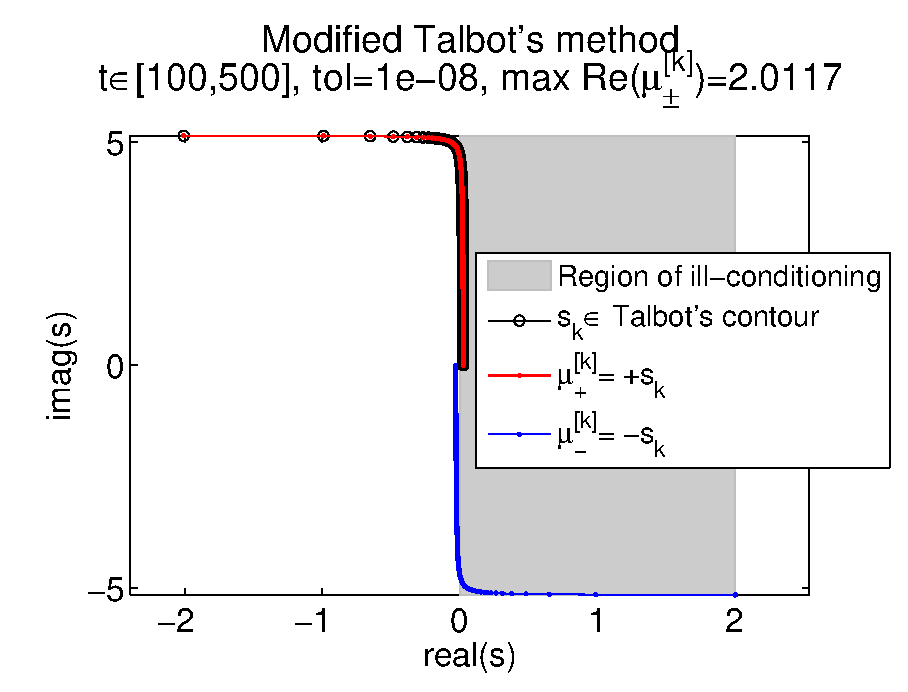
\includegraphics[width=0.25\textwidth]{./FIGS/EX4a/EX4a_illcond_tol2_t100_Talbot1.eps} &
\includegraphics[width=0.25\textwidth]{./FIGS/EX4a/EX4a_illcond_tol2_t100_Talbot2.eps}
\end{tabular}
\caption{\small Regions of ill-conditioning of problem (\ref{EX4a:ODE}) for ${\tt tol}=10^{-8}$.}
\label{EX4a_a1}
\end{figure}
%-------------------------------------------------------------------
%-------------------------------------------------------------------
\begin{figure}[htb]
\centering
\begin{tabular}{cc}
\includegraphics[width=0.25\textwidth]{./FIGS/EX4a/EX4a_illcond_tol4_t1_Talbot1.eps} &
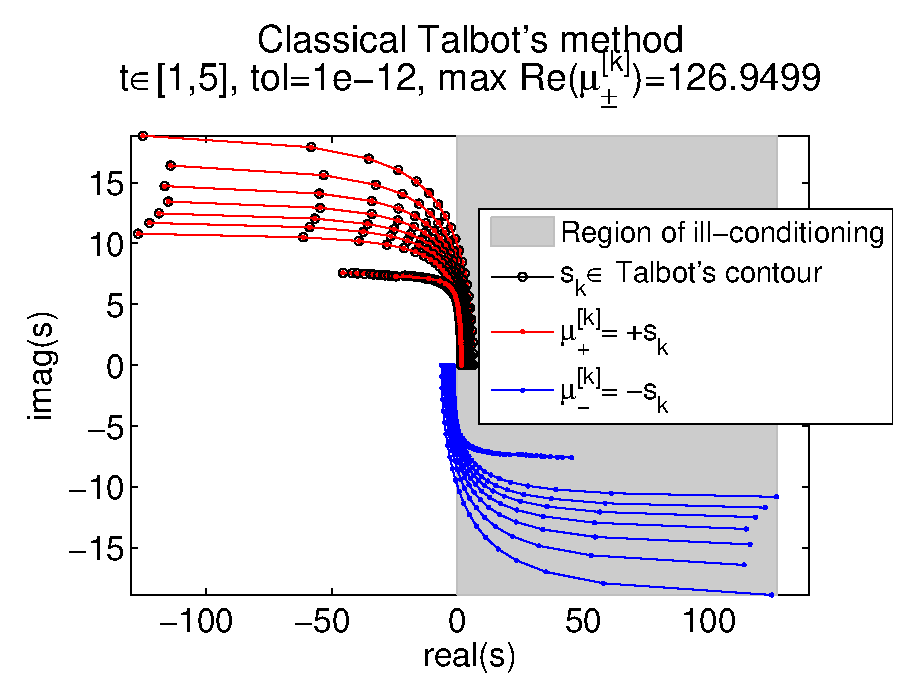
\includegraphics[width=0.25\textwidth]{./FIGS/EX4a/EX4a_illcond_tol4_t1_Talbot2.eps} \\
\includegraphics[width=0.25\textwidth]{./FIGS/EX4a/EX4a_illcond_tol4_t100_Talbot1.eps} &
\includegraphics[width=0.25\textwidth]{./FIGS/EX4a/EX4a_illcond_tol4_t100_Talbot2.eps}
\end{tabular}
\caption{\small Regions of ill-conditioning of problem (\ref{EX4a:ODE}) for ${\tt tol}=10^{-12}$.}
\label{EX4a_a2}
\end{figure}
%-------------------------------------------------------------------

\noindent As in Example 3a, the {\em classical method} results more ill-conditioned than the {\em modified method}
and the ill-conditioning decreases as $t$ increases.
However, Figs.~\ref{EX4a_a1} and \ref{EX4a_a2} show that, since {\tt NOPTS} changes with {\tt tol} (due to the
complex singularities), consequently the ill-conditioning increases with {\tt tol} (besides with $x$).

When this IVP is solved by means of {\tt ode45.m}, in the MATLAB Command Window, the sample code has a driver
program written as a MATLAB script ({\tt MAIN.m}) that calls C-mex functions for accuracy and for partial
elapsed times.
Otherwise it is entirely written in C and makes use of {\tt ode.c}.

\newpage
About accuracy the problem (\ref{EX4a:PDE}) has been solved, at first, for ${\tt NXval}=9\; x\in[0,1]$,
${\tt NTval}=5\; t\in[100,500]$ and ${\tt tol}=10^{-12}$; output results are reported in the following.
\begin{lstlisting}
             Ex. 4a: output from ./1SEQ/LTS2_ode/SEQ_main_ACCURACY.c
          LT samples computed by solving ODE problems by means of ode.c
           5 t in [100, 500],    9 x in [0, 1],    tol=1.000000e-012
====================================================================================
RELERR1 = [ %  Tval(1)    Tval(2)    ...    Tval(5)
  3.027651e-014  4.149160e-013  3.990648e-013  2.022519e-011  9.005538e-012% Xval(1)
  2.064593e-014  8.395187e-014  7.392255e-013  9.876384e-012  1.209567e-012% Xval(2)
  1.851265e-015  1.476978e-015  1.063776e-012  1.497035e-012  1.611262e-011% Xval(3)
  5.073628e-014  1.398595e-014  1.018135e-013  9.416037e-012  5.204663e-011% Xval(4)
  8.224403e-013  7.277526e-015  3.348585e-012  9.170879e-012  1.762521e-010% Xval(5)
  3.521410e-013  2.044974e-014  4.360682e-012  1.037631e-011  2.730738e-010% Xval(6)
  1.901604e-013  9.680986e-014  2.321052e-012  1.025391e-011  8.159249e-011% Xval(7)
  1.389670e-013  2.288526e-013  1.910029e-012  2.399973e-012  3.161025e-011% Xval(8)
  1.003246e-013  6.945304e-013  5.584575e-013  2.007232e-011  1.511929e-012% Xval(9)
  ];
RELERR2 = [ %  Tval(1)    Tval(2)    ...    Tval(5)
  2.879041e-012  5.524007e-010  1.253451e-012  1.667625e-012  2.918517e-013% Xval(1)
  3.676904e-012  7.177901e-011  7.450403e-013  1.840197e-012  4.786690e-014% Xval(2)
  4.930632e-012  2.927371e-011  3.456172e-013  9.569925e-013  2.922924e-013% Xval(3)
  5.079396e-012  1.498015e-011  1.284907e-012  5.163980e-013  1.205317e-013% Xval(4)
  1.250581e-011  4.705777e-012  6.411816e-012  6.690783e-013  1.086972e-012% Xval(5)
  2.763479e-012  4.022441e-012  5.873314e-012  4.266178e-013  6.146832e-013% Xval(6)
  5.893588e-013  1.425439e-011  2.752291e-012  3.927406e-013  2.248001e-013% Xval(7)
  1.294031e-012  3.415270e-011  2.545970e-012  9.209089e-013  3.765228e-013% Xval(8)
  1.751937e-012  1.191074e-010  1.951996e-012  3.237772e-013  7.029774e-016% Xval(9)
  ];
\end{lstlisting}
\begin{lstlisting}
             Ex. 4a: output from ./1SEQ/LTS3_mex/MAIN.m
          LT samples computed by solving ODE problems by means of MATLAB ode45.m
           5 t in [100, 500],    9 x in [0, 1],    tol=1.000000e-012
====================================================================================
RELERR1 = [ %  Tval(1)    Tval(2)    ...    Tval(5)
  3.027651e-14 4.334605e-13 4.021981e-13 2.028480e-11 9.077428e-12% Xval(1)
  1.201321e-13 1.513429e-13 7.343052e-13 2.142091e-12 1.000807e-11% Xval(2)
  1.700316e-13 4.366933e-13 9.643215e-13 5.022477e-13 1.091848e-11% Xval(3)
  2.841703e-13 1.108025e-13 1.093880e-12 6.302184e-13 1.326704e-11% Xval(4)
  9.199041e-13 1.857910e-13 1.018785e-12 8.025274e-12 1.591776e-12% Xval(5)
  1.674144e-14 2.796996e-13 4.345188e-12 3.421876e-12 9.429604e-11% Xval(6)
  1.700706e-13 3.872394e-13 6.912146e-14 1.952046e-11 4.069373e-11% Xval(7)
  2.707949e-13 5.616565e-13 5.050868e-13 6.302570e-12 1.353165e-10% Xval(8)
  3.700673e-13 5.804259e-13 6.851164e-13 1.023227e-11 9.024121e-12% Xval(9)
  ];
RELERR2 = [ %  Tval(1)    Tval(2)    ...    Tval(5)
  2.879893e-12 5.523644e-10 1.254305e-12 1.652533e-12 2.901359e-13% Xval(1)
  4.729393e-12 7.377025e-11 9.376743e-13 7.867714e-13 1.526089e-13% Xval(2)
  4.201518e-12 2.878615e-11 3.309647e-13 9.524850e-13 4.460858e-15% Xval(3)
  5.717190e-12 1.346762e-11 3.368536e-12 7.552971e-13 4.530831e-13% Xval(4)
  1.917951e-11 4.677309e-12 1.259187e-11 1.086740e-12 6.668524e-13% Xval(5)
  1.820251e-12 4.775343e-12 3.315304e-12 1.655922e-14 7.218049e-12% Xval(6)
  4.658758e-13 1.597785e-11 3.279018e-12 3.065196e-12 6.035773e-13% Xval(7)
  2.436170e-12 3.672136e-11 2.335008e-12 3.965985e-13 3.021642e-12% Xval(8)
  2.976796e-12 1.276722e-10 1.795662e-12 8.646496e-13 5.623819e-14% Xval(9)
  ];
\end{lstlisting}

\noindent To highlight the effects of ill-conditioning, let us repeat the accuracy test in a larger interval for
$x$, namely ${\tt NXval}=9\; x\in[0,2\pi]$, ${\tt NTval}=5\; t\in[1,5]$ and ${\tt tol}=10^{-8}$.
The following output displays the relative errors that become very large in both {\em modified} and {\em
classical methods}. The same occurs for {\tt ode45.m}.
For ${\tt tol}=10^{-12}$, {\tt ode.c} returns the error indicator {\tt iflag = 4} to denote that the maximum
number of iterations has been reached but the accuracy cannot be satisfied.
\begin{lstlisting}
             Ex. 4a: output from ./1SEQ/LTS2_ode/SEQ_main_ACCURACY.c
          LT samples computed by solving ODE problems by means of ode.c
           5 t in [1, 5],    9 x in [0, 6.28319],    tol=1.000000e-008
====================================================================================
RELERR1 = [ %  Tval(1)    Tval(2)    ...    Tval(5)
  3.093631e-009  5.437069e-013  1.144925e-013  1.101796e-014  9.469254e-013% Xval(1)
  4.980387e-008  5.936257e-007  2.013549e-006  2.935761e-006  8.546006e-006% Xval(2)
  8.684332e-005  4.360408e-007  4.861166e-006  1.075217e-005  6.865145e-004% Xval(3)
  3.094571e+006  5.187424e-006  5.813287e-005  1.736777e-003  4.550455e-002% Xval(4)
  5.872744e+016  2.661721e+004  5.523072e-004  1.468263e-003  6.089902e-002% Xval(5)
  3.231969e+025  1.514702e+013  7.338038e+000  2.578236e-002  2.688684e-002% Xval(6)
  6.719380e+034  1.456438e+022  3.465458e+010  8.143229e-002  1.544710e+000% Xval(7)
  2.377552e+044  4.479504e+031  2.921515e+020  2.419309e+008  2.418685e+001% Xval(8)
  1.644721e+054  6.997059e+041  6.670973e+029  9.316427e+016  2.342507e+005% Xval(9)
  ];

RELERR2 = [ %  Tval(1)    Tval(2)    ...    Tval(5)
  2.717105e-010  3.489286e-010  7.797479e-012  1.490497e-011  1.580558e-010% Xval(1)
  3.586194e-005  2.313158e-007  2.464469e-006  2.284720e-006  2.834271e-006% Xval(2)
  3.226452e+012  9.550152e-005  4.071799e-006  1.184580e-005  1.061577e-005% Xval(3)
  2.237310e+040  1.399760e+004  1.155896e-004  2.778497e-005  4.817538e-005% Xval(4)
  2.693794e+072  2.140398e+033  7.203667e-004  4.969134e-005  1.579482e-006% Xval(5)
  1.296906e+101  5.700646e+061  1.391436e-001  4.233518e-004  2.018923e-006% Xval(6)
  2.503119e+130  3.859857e+090  1.509136e+007  2.580542e-003  5.252524e-004% Xval(7)
  3.693363e+160  4.247981e+119  2.920552e+015  9.783253e+001  2.586602e-002% Xval(8)
  1.807085e+190  1.246726e+147  1.486383e+023  1.135093e+007  6.169985e-002% Xval(9)
  ];
\end{lstlisting}
The values of the leftmost columns in {\tt RELERR2} with respect to those in {\tt RELERR1} confirm that the
ill-conditioning of the {\em classical method} overcomes that one of the {\em modified method}.
\\
With larger values of $t$ the ill-conditioning disappears and we are able to set ${\tt tol}=10^{-12}$,
as reported by the following output.
\begin{lstlisting}
             Ex. 4a: output from ./1SEQ/LTS2_ode/SEQ_main_ACCURACY.c
          LT samples computed by solving ODE problems by means of ode.c
           5 t in [100, 500],    9 x in [0, 6.28319],    tol=1.000000e-012
====================================================================================
RELERR1 = [ %  Tval(1)    Tval(2)    ...    Tval(5)
  3.027651e-014  4.149160e-013  3.990648e-013  2.022519e-011  9.005538e-012% Xval(1)
  3.977266e-015  3.046808e-013  7.085691e-013  7.452627e-012  6.342782e-012% Xval(2)
  3.766269e-012  2.726805e-013  1.201998e-011  7.131309e-012  1.405789e-009% Xval(3)
  5.274426e-014  1.315244e-013  5.873009e-012  5.773162e-011  1.642108e-010% Xval(4)
  1.060476e-013  3.788860e-012  8.461518e-012  1.863135e-010  1.203404e-010% Xval(5)
  1.925552e-013  2.461396e-013  5.852296e-012  1.360527e-011  1.344900e-010% Xval(6)
  4.723243e-012  6.437228e-013  2.216113e-011  3.523847e-011  1.846323e-009% Xval(7)
  7.270567e-015  1.347527e-012  7.907373e-012  5.185673e-011  2.755854e-010% Xval(8)
  7.101600e-014  2.283512e-011  7.404367e-012  6.996816e-011  1.727209e-011% Xval(9)
  ];

RELERR2 = [ %  Tval(1)    Tval(2)    ...    Tval(5)
  2.879041e-012  5.524007e-010  1.253451e-012  1.667625e-012  2.918517e-013% Xval(1)
  6.132333e-012  1.939768e-011  1.360978e-012  1.921527e-012  1.011510e-012% Xval(2)
  1.346141e-010  6.524642e-012  3.401012e-014  2.592041e-013  1.884347e-011% Xval(3)
  7.055338e-012  3.052568e-011  1.871777e-012  3.737006e-012  6.399301e-012% Xval(4)
  4.258650e-012  5.432978e-010  2.004103e-012  3.384907e-011  4.234668e-012% Xval(5)
  5.856023e-012  1.692979e-011  7.438349e-013  7.157769e-014  7.055653e-013% Xval(6)
  2.601251e-010  6.054705e-012  1.856841e-011  3.526026e-012  3.221228e-011% Xval(7)
  1.718119e-011  3.032081e-011  4.028155e-012  9.481414e-012  8.791478e-012% Xval(8)
  9.026655e-012  5.996075e-010  3.211284e-012  3.376682e-011  6.390193e-012% Xval(9)
  ];
\end{lstlisting}

About efficiency, the computational cost of the entire algorithm depends on the time required by each step of
the algorithm, namely the evaluation of method's parameters ({\tt PAR} step), the computation of Laplace
Transform samples ({\tt LTS} step) and the evaluation of approximating summations ({\tt SUM} step).
Partial and total elapsed times are reported in the following for {\tt NXval} $x\in[0,1]$, {\tt NTval}
$t\in[100,500]$ and ${\tt tol}=10^{-12}$.
\begin{lstlisting}
             Ex. 4a: output from ./1SEQ/LTS2_ode/SEQ_main_TIMES.c
          LT samples computed by solving ODE problems by means of ode.c
          t in [100, 500],    x in [0, 1],    tol=1.000000e-12
====================================================================================
PARtime1 = [%            5             20            120  = NXval
              1.407130e-006  2.430497e-006  3.453864e-006 % NTval =   5
              1.726932e-006  2.494457e-006  3.709705e-006 % NTval =  20
              1.599011e-006  2.814259e-006  3.773666e-006 % NTval = 120
           ];
LTStime1 = [%            5             20            120  = NXval
              3.298386e-001  9.712600e-001  3.828374e+000 % NTval =   5
              3.300135e-001  9.717514e-001  3.799555e+000 % NTval =  20
              3.331108e-001  9.722766e-001  3.800905e+000 % NTval = 120
           ];
SUMtime1 = [%            5             20            120  = NXval
              3.920839e-003  1.563526e-002  9.473666e-002 % NTval =   5
              1.566033e-002  6.296835e-002  3.777628e-001 % NTval =  20
              9.413320e-002  3.776602e-001  2.262845e+000 % NTval = 120
           ];
TOTtime1 = [%            5             20            120  = NXval
              3.337608e-001  9.868977e-001  3.923114e+000 % NTval =   5
              3.456755e-001  1.034722e+000  4.177322e+000 % NTval =  20
              4.272455e-001  1.349940e+000  6.063753e+000 % NTval = 120
           ];
PARtime2 = [%            5             20            120  = NXval
              5.500598e-006  1.087327e-005  1.439110e-005 % NTval =   5
              2.296180e-005  3.600973e-005  6.389648e-005 % NTval =  20
              1.443587e-004  2.213031e-004  3.778143e-004 % NTval = 120
           ];
LTStime2 = [%            5             20            120  = NXval
              1.808723e+000  5.446123e+000  2.101817e+001 % NTval =   5
              6.869331e+000  2.014425e+001  7.953745e+001 % NTval =  20
              4.030278e+001  1.189850e+002  4.667229e+002 % NTval = 120
           ];
SUMtime2 = [%            5             20            120  = NXval
              4.277226e-003  1.737933e-002  1.040137e-001 % NTval =   5
              1.613914e-002  6.438840e-002  3.907388e-001 % NTval =  20
              9.560039e-002  3.815985e-001  2.308894e+000 % NTval = 120
           ];
TOTtime2 = [%            5             20            120  = NXval
              1.813006e+000  5.463513e+000  2.112220e+001 % NTval =   5
              6.885493e+000  2.020868e+001  7.992826e+001 % NTval =  20
              4.039852e+001  1.193668e+002  4.690321e+002 % NTval = 120
           ];
\end{lstlisting}
\begin{lstlisting}
             Ex. 4a: output from ./1SEQ/LTS3_mex/MAIN.m
          LT samples computed by solving ODE problems by means of MATLAB ode45.m
          t in [100, 500],    x in [0, 1],    tol=1.000000e-12
====================================================================================
PARtime1 = [%            5             20            120  = NXval
              2.238595e-06   2.558394e-06   2.718293e-06  % NTval =   5
              2.718293e-06   2.398494e-06   2.878193e-06  % NTval =  20
              2.398486e-06   2.398486e-06   2.718285e-06  % NTval = 120
           ];
LTStime1 = [%            5             20            120  = NXval
              4.191149e+01   4.250662e+01   4.656570e+01  % NTval =   5
              4.185615e+01   4.251340e+01   4.659168e+01  % NTval =  20
              4.171219e+01   4.268450e+01   4.683502e+01  % NTval = 120
           ];
SUMtime1 = [%            5             20            120  = NXval
              3.664579e-03   1.469493e-02   8.854233e-02  % NTval =   5
              1.470485e-02   5.895419e-02   3.551892e-01  % NTval =  20
              8.806887e-02   3.530372e-01   2.125875e+00  % NTval = 120
           ];
TOTtime1 = [%            5             20            120  = NXval
              4.191516e+01   4.252132e+01   4.665424e+01  % NTval =   5
              4.187086e+01   4.257236e+01   4.694688e+01  % NTval =  20
              4.174496e+01   4.303754e+01   4.896090e+01  % NTval = 120
           ];
PARtime2 = [%            5             20            120  = NXval
              9.593977e-06   9.753876e-06   1.151277e-05  % NTval =   5
              3.709671e-05   3.693681e-05   5.292677e-05  % NTval =  20
              2.232191e-04   2.291354e-04   2.563343e-04  % NTval = 120
           ];
LTStime2 = [%            5             20            120  = NXval
              2.292385e+02   2.327408e+02   2.551893e+02  % NTval =   5
              8.660459e+02   8.791061e+02   1.213027e+03  % NTval =  20
              5.124863e+03   5.218308e+03   5.739994e+03  % NTval = 120
           ];
SUMtime2 = [%            5             20            120  = NXval
              4.013160e-03   1.621350e-02   9.690124e-02  % NTval =   5
              1.519462e-02   6.068254e-02   3.656389e-01  % NTval =  20
              9.000544e-02   3.595750e-01   2.168932e+00  % NTval = 120
           ];
TOTtime2 = [%            5             20            120  = NXval
              2.292426e+02   2.327571e+02   2.552862e+02  % NTval =   5
              8.660611e+02   8.791668e+02   1.213392e+03  % NTval =  20
              5.124953e+03   5.218668e+03   5.742163e+03  % NTval = 120
           ];
\end{lstlisting}
These results are summarized together in Fig.~\ref{EX4a_times3D_tol4}.
%-------------------------------------------------------------------
\begin{figure}[htb]
\centering
\begin{tabular}{cc}
\includegraphics[width=0.25\textwidth]{./FIGS/EX4a/EX4a_times3D_tol4_1.eps} &
\includegraphics[width=0.25\textwidth]{./FIGS/EX4a/EX4a_times3D_tol4_3.eps} \\
\includegraphics[width=0.25\textwidth]{./FIGS/EX4a/EX4a_times3D_tol4_2.eps} &
\includegraphics[width=0.25\textwidth]{./FIGS/EX4a/EX4a_times3D_tol4_4.eps}
\end{tabular}
\caption{\small Mesh plot of execution times in solving (\ref{EX4a:PDE}).}
\label{EX4a_times3D_tol4}
\end{figure}
%-------------------------------------------------------------------

\newpage
\noindent Two remarks have to be done.
The first is that the evaluation of the LT samples is always the most expensive step.
The second is that the C code is much more efficient than the mixed C/MATLAB code.



%\newpage
%%%%%%%%%%%%%%%%%%%%%%%%%%%%%%%%%%%%%%%%%%%%%%%%%%%%%%%%%%%%%%%%%%%%%%%%%%%%%%%%%%
\subsection{Example 4b}
%%%%%%%%%%%%%%%%%%%%%%%%%%%%%%%%%%%%%%%%%%%%%%%%%%%%%%%%%%%%%%%%%%%%%%%%%%%%%%%%%%
The sample code is located in the sub-folder {\tt ex4b\_BVP/1SEQ} of the main folder.
\\
Now we add a boundary condition to (\ref{EX4:PDE}) as follows:
% an initial condition in (\ref{EX4a:ODE}) into a boundary condition as follows.
\begin{equation}\label{EX4b}
\left\{\begin{array}{lll}
\dfrac{\partial^2 u}{\partial t^2} = \dfrac{\partial^2 u}{\partial x^2}, &  0<x<L, & t > 0 \\[4pt]
\begin{array}{lcl}
  u(x,0^+)   &=& \dfrac{x\sin(3x)}{6}, \\[8pt]
  \dfrac{\partial u}{\partial t}(x,0^+) &=& \dfrac{\sin(3x)}{6} + \dfrac{x\cos(3x)}{2},
\end{array} \\[24pt]
\begin{array}{lcl}
  u(0,t) &=& \dfrac{t\sin(3t)}{6}, \\[8pt]
  u(L,t) &=& \dfrac{(L+t)\sin[3(L+t)]}{6}
\end{array}
\end{array}\right.
\end{equation}
The analytical solution of (\ref{EX4b}) is the function (\ref{SOLUTION:EX1b}).
\\
The {\em Laplace Transform method} applied to (\ref{EX4b}) gives the following BVP:
\begin{equation}\label{WAVE:ODE:4b}
\left\{\begin{array}{lcll}
%U''       &=& s^2 U - \dfrac{sx\sin(3x)}{6} - \dfrac{\sin(3x)}{6} - \dfrac{x\cos(3x)}{2},  & 0 < x < 2\pi \\[8pt]
 U'' &=& s^2 U - (sx+1)\dfrac{\sin(3x)}{6} - x\dfrac{\cos(3x)}{2},  & 0 < x < L \\[8pt]
U(0) &=& \dfrac{s}{(s^2 + 9)^2}, \\[8pt]
U(L) &=& \dfrac{s\cos(3L)-3\sin(3L)}{(s^2 + 9)^2} + \dfrac{(sL+1)\sin(3L)+3L\cos(3L)}{6(s^2 + 9)}
\end{array}\right.
\end{equation}
whose solution is given by (\ref{LT_SOLUTION:EX1b}). Problem (\ref{WAVE:ODE:4b}) is similar
to (\ref{HEAT:ODE:case1}) so that we may apply the same algorithms. 
Each problem (\ref{WAVE:ODE:4b}), for a given $s_k$ on the Talbot contour, is solved by a call to
{\tt twpbvp.f} or to {\tt bvp5c.m} inside a for-loop. The main difference is that, now, the values of
{\tt NOPTS} may become large and we have to solve a lot of BVPs (\ref{WAVE:ODE:4b}) and,
consequently, times for running the sequential code may grow very much.

About accuracy, the problem (\ref{EX4a:PDE}) has been solved for ${\tt NXval}=9\; x\in[0,1]$,
${\tt NTval}=5\; t\in[100,500]$ and ${\tt tol}=10^{-6}$; output results are reported in the following.
\newpage
\begin{lstlisting}
             Ex. 4b: output from ./1SEQ/LTS2_twpbvp/SEQ_main_ACCURACY.c
          LT samples computed by solving ODE problems by means of twpbvp.f
           5 t in [100, 500],    9 x in [0, 1],    tol=1.000000e-006
====================================================================================
RELERR1 = [ %  Tval(1)    Tval(2)    ...    Tval(5)
  3.144474e-010  8.805508e-009  1.113552e-010  2.558448e-009  7.404351e-011% Xval(1)
  6.844319e-010  1.911101e-008  3.746961e-008  4.213526e-007  3.628944e-007% Xval(2)
  1.914527e-009  1.702886e-008  8.401954e-008  3.556404e-007  7.741197e-007% Xval(3)
  4.305869e-009  1.607498e-008  1.713168e-007  3.293198e-007  1.473289e-006% Xval(4)
  2.287966e-008  1.524644e-008  6.559570e-007  3.086131e-007  4.470549e-006% Xval(5)
  7.079401e-009  1.428269e-008  3.466892e-007  2.861820e-007  3.696920e-006% Xval(6)
  2.517262e-009  1.287919e-008  1.072366e-007  2.557196e-007  9.647134e-007% Xval(7)
  1.063584e-009  1.010834e-008  3.946312e-008  2.003902e-007  3.305823e-007% Xval(8)
  2.122862e-010  2.200135e-009  7.142842e-011  1.031300e-009  4.959558e-011% Xval(9)
  ];
RELERR2 = [ %  Tval(1)    Tval(2)    ...    Tval(5)
  2.805007e-008  2.661977e-006  6.567016e-009  2.989376e-009  4.032049e-014% Xval(1)
  6.056661e-008  4.236631e-007  1.023113e-009  2.761364e-008  2.321625e-008% Xval(2)
  1.034934e-007  2.133908e-007  1.047832e-008  2.299510e-008  5.182629e-008% Xval(3)
  1.913554e-007  1.358716e-007  2.798635e-008  1.656018e-005  1.688401e-005% Xval(4)
  8.906814e-007  8.512574e-008  1.237379e-007  1.079182e-005  6.102908e-005% Xval(5)
  2.398298e-007  3.864460e-008  7.300191e-008  1.838950e-008  2.860773e-007% Xval(6)
  6.717569e-008  1.889680e-008  2.537217e-008  1.636817e-008  7.866204e-008% Xval(7)
  1.062831e-008  1.237338e-007  1.145649e-008  1.264528e-008  2.837610e-008% Xval(8)
  2.476281e-008  5.814379e-007  3.059893e-009  1.080835e-009  1.792592e-014% Xval(9)
  ];
\end{lstlisting}
\begin{lstlisting}
             Ex. 4b: output from ./1SEQ/LTS3_mex/MAIN.m
          LT samples computed by solving ODE problems by means of MATLAB bvp5c.m
           5 t in [100, 500],    9 x in [0, 1],    tol=1.000000e-06
====================================================================================
RELERR1 = [ %  Tval(1)    Tval(2)    ...    Tval(5)
  3.144474e-10 8.805508e-09 1.113529e-10 2.558444e-09 7.402498e-11% Xval(1)
  2.767127e-10 1.146434e-08 6.093480e-10 1.264712e-08 3.378168e-09% Xval(2)
  9.171023e-10 1.002416e-08 1.375946e-09 9.997878e-09 5.219427e-09% Xval(3)
  2.032185e-09 9.408790e-09 2.675356e-09 9.210693e-09 1.123032e-08% Xval(4)
  1.031465e-08 8.948293e-09 1.176839e-08 1.123510e-08 3.454459e-07% Xval(5)
  3.022345e-09 8.318076e-09 4.634213e-09 8.026139e-09 2.600808e-08% Xval(6)
  1.035081e-09 7.456947e-09 1.328338e-09 7.170198e-09 6.428849e-09% Xval(7)
  4.660593e-10 5.714642e-09 4.837152e-10 5.426027e-09 3.136974e-09% Xval(8)
  2.122871e-10 2.200136e-09 7.142929e-11 1.031317e-09 4.956465e-11% Xval(9)
  ];
RELERR2 = [ %  Tval(1)    Tval(2)    ...    Tval(5)
  2.805007e-08 2.661977e-06 6.567017e-09 2.989360e-09 4.032049e-14% Xval(1)
  3.562318e-08 4.158615e-07 1.504575e-08 1.107960e-08 8.810678e-10% Xval(2)
  4.567902e-08 2.064771e-07 2.613252e-08 9.803066e-09 1.822119e-09% Xval(3)
  6.731121e-08 1.292734e-07 4.787468e-08 9.201103e-09 3.374678e-09% Xval(4)
  2.414566e-07 7.875520e-08 1.717266e-07 9.113081e-09 9.766424e-09% Xval(5)
  4.081199e-08 3.254614e-08 8.586399e-08 8.437514e-09 7.917976e-09% Xval(6)
  2.037372e-09 2.454174e-08 2.461903e-08 7.732808e-09 1.979961e-09% Xval(7)
  1.599537e-08 1.284421e-07 7.236181e-09 6.364366e-09 6.400027e-10% Xval(8)
  2.476281e-08 5.814379e-07 3.059894e-09 1.080821e-09 2.056209e-14% Xval(9)
  ];
\end{lstlisting}
Only for the mixed C/MATLAB sample code, we report the relative errors also for ${\tt tol}=10^{-12}$.
The usual selection of parameters and dimension of working areas of {\tt twpbvp.f} do not allow to satisfy
higher accuracy requirements. If we enlarge the interval for $x$, higher accuracy requirements produce
an error message due to the maximum mesh size and the program exits with the error flag {\tt iflbvp=1}.
To have a larger mesh size we need to increase again the size of some working arrays.
In {\tt SEQ\_LTsamples\_twpbvp.c}, the function that calls {\tt twpbvp.f}, as dimensions of some working areas
we set {\tt lwrkfl = 30000} and {\tt lwrkin = 18000} to manage till 120 values for $x\in[0,1]$.
The value of {\tt nmax} (maximum mesh size) depends on these values, and the flag {\tt iflbvp = 1}
indicates that the function was interrupted since the next iteration would require a mesh size greater
than {\tt nmax}.
\begin{lstlisting}
             Ex. 4b: output from ./1SEQ/LTS3_mex/MAIN.m
          LT samples computed by solving ODE problems by means of MATLAB bvp5c.m
           5 t in [100, 500],    9 x in [0, 1],    tol=1.000000e-12
====================================================================================
RELERR1 = [ %  Tval(1)    Tval(2)    ...    Tval(5)
  3.027651e-14 4.334605e-13 4.021981e-13 2.028480e-11 9.077428e-12% Xval(1)
  1.054984e-14 9.346204e-15 5.163247e-13 2.077265e-12 1.130931e-11% Xval(2)
  1.737341e-14 1.723142e-14 6.626619e-13 1.175436e-12 1.396036e-11% Xval(3)
  7.604556e-14 2.857474e-14 9.542665e-13 2.251169e-12 1.845943e-11% Xval(4)
  5.491986e-13 3.574550e-14 2.555072e-12 2.931611e-12 3.854527e-11% Xval(5)
  2.121217e-13 4.133925e-14 8.067872e-13 3.525807e-12 1.546485e-11% Xval(6)
  9.992949e-14 4.972387e-14 1.478534e-15 4.171684e-12 1.809309e-12% Xval(7)
  6.166739e-14 6.324871e-14 2.269157e-13 5.313972e-12 6.358420e-12% Xval(8)
  3.636500e-14 1.287443e-13 3.613037e-13 9.568859e-12 8.753299e-12% Xval(9)
  ];
RELERR2 = [ %  Tval(1)    Tval(2)    ...    Tval(5)
  2.879893e-12 5.523644e-10 1.254305e-12 1.652533e-12 2.901359e-13% Xval(1)
  3.424502e-12 7.305698e-11 7.392255e-13 8.480171e-13 2.841987e-13% Xval(2)
  4.159793e-12 3.045497e-11 6.318916e-14 4.914989e-13 2.744490e-13% Xval(3)
  5.693176e-12 1.477856e-11 1.247542e-12 3.618745e-13 2.652666e-13% Xval(4)
  1.803381e-11 4.552093e-12 8.691008e-12 2.960504e-13 2.156699e-13% Xval(5)
  1.977393e-12 4.781940e-12 6.773823e-12 2.337900e-13 3.693850e-13% Xval(6)
  1.061816e-12 1.628832e-11 3.102703e-12 1.607598e-13 3.138033e-13% Xval(7)
  2.042779e-12 3.717707e-11 2.068548e-12 2.356031e-14 2.966352e-13% Xval(8)
  2.645447e-12 1.281820e-10 1.456071e-12 4.453832e-13 2.991169e-13% Xval(9)
  ];
\end{lstlisting}
We must not forget that the analytical solution $u(x,t)$ of (\ref{EX4b}) has a wave behavior that increases the number of oscillations with both $x$ and $t$; also its LT function is oscillating with $x$.
\\[.1in]
\indent This example emphasizes some questions about {\tt twpbvp.f} which don't arise in Example 3b.
We mention them briefly, since we are concerned with the application of Talbot's methods and not with the usage
of third-party software. The main problem is due to the the number of mesh points for $x$ returned by
{\tt twpbvp.f}: we are able to give in input to the function our mesh points for $x$, but it may return a
different mesh size and different mesh points so that the LT samples are not computed where we want.
In addition, since a different BVP is solved for each point on the Talbot contour, the returned mesh size may
change from one BVP to another so that it is not possible to put all the LT samples into the same matrix,
required by the inversion method for the summation step.
In Example 3b (sect. \ref{EX3b}) the mesh size returned by {\tt twpbvp.f} ({\tt nmsh}) was always equal to our
mesh size ({\tt NXval}) and the above problem did not occur.
\\
The oscillating test function of this example often produces ${\tt nmsh}>{\tt NXval}$: in this case, for
the application of Talbot's method, we introduce a data fitting based on the {\em third degree Hermite
interpolating polynomial}. For each desired grid point $x$ it, at first, locates the interval of the
mesh returned by {\tt twpbvp.f} and containing $x$, and then approximates the Laplace Transform at $x$,
exploiting function and derivative values known at the endpoints of the interval from the differential problem. 
Of course, this fitting introduces a further delay.
\\[.15in]
\indent About efficiency, the computational cost of the entire algorithm depends on the time required by each step of
the algorithm, namely the evaluation of method's parameters ({\tt PAR} step), the computation of Laplace
Transform samples ({\tt LTS} step) and the evaluation of approximating summations ({\tt SUM} step).
Partial and total elapsed times are reported in the following for {\tt NXval} $x\in[0,1]$, {\tt NTval}
$t\in[100,500]$ and ${\tt tol}=10^{-12}$.
\begin{lstlisting}
             Ex. 4b: output from ./1SEQ/LTS2_twpbvp/SEQ_main_TIMES.c
          LT samples computed by solving ODE problems by means of twpbvp.f
          t in [100, 500],    x in [0, 1],    tol=1.000000e-12
====================================================================================
PARtime1 = [%             5             20            120   = NXval
              2.494426e-006  1.343152e-006  3.070063e-006   % NTval =   5
              1.407112e-006  1.279193e-006  5.884287e-006   % NTval =  20
              1.662951e-006  1.854830e-006  3.709659e-006   % NTval = 120
           ];
LTStime1 = [%             5             20            120   = NXval
              4.628059e-001  3.615970e-001  7.570526e-001   % NTval =   5
              4.513896e-001  3.611273e-001  7.577082e-001   % NTval =  20
              4.516904e-001  3.613177e-001  7.560800e-001   % NTval = 120
           ];
SUMtime1 = [%             5             20            120   = NXval
              3.990442e-003  1.557577e-002  9.387663e-002   % NTval =   5
              1.557507e-002  6.275560e-002  3.748869e-001   % NTval =  20
              9.347618e-002  3.751674e-001  2.249595e+000   % NTval = 120
           ];
TOTtime1 = [%             5             20            120   = NXval
              4.667988e-001  3.771741e-001  8.509323e-001   % NTval =   5
              4.669661e-001  4.238841e-001  1.132601e+000   % NTval =  20
              5.451682e-001  7.364869e-001  3.005679e+000   % NTval = 120
           ];
PARtime2 = [%             5             20            120   = NXval
              6.907641e-006  8.698511e-006  1.221629e-005   % NTval =   5
              2.289755e-005  2.046708e-005  3.907934e-005   % NTval =  20
              1.400716e-004  1.258726e-004  2.660081e-004   % NTval = 120
           ];
LTStime2 = [%             5             20            120   = NXval
              2.477966e+000  1.981000e+000  4.145244e+000   % NTval =   5
              9.346294e+000  7.473008e+000  1.565017e+001   % NTval =  20
              5.533169e+001  4.428304e+001  9.267324e+001   % NTval = 120
           ];
SUMtime2 = [%             5             20            120   = NXval
              4.284081e-003  1.704691e-002  1.031395e-001   % NTval =   5
              1.611009e-002  6.421784e-002  3.878312e-001   % NTval =  20
              9.527178e-002  3.802253e-001  2.294577e+000   % NTval = 120
           ];
TOTtime2 = [%             5             20            120   = NXval
              2.482257e+000  1.998056e+000  4.248395e+000   % NTval =   5
              9.362427e+000  7.537247e+000  1.603804e+001   % NTval =  20
              5.542710e+001  4.466339e+001  9.496808e+001   % NTval = 120
           ];
\end{lstlisting}
\begin{lstlisting}
             Ex. 4b: output from ./1SEQ/LTS3_mex/MAIN.m
          LT samples computed by solving ODE problems by means of MATLAB bvp5c.m
          t in [100, 500],    x in [0, 1],    tol=1.000000e-12
====================================================================================
PARtime1 = [%            5             20            120  = NXval
               2.110668e-06 2.430466e-06 7.675157e-06  %   5 = NTval
               3.197982e-06 3.006103e-06 3.325901e-06  %  20 = NTval
               2.814224e-06 3.006103e-06 3.006103e-06  % 120 = NTval
           ];
LTStime1 = [ %            5           20          120  = NXval
               3.135684e+02 3.724105e+02 3.150983e+02  %   5 = NTval
               3.269009e+02 3.887075e+02 3.275121e+02  %  20 = NTval
               3.372510e+02 4.008671e+02 3.278941e+02  % 120 = NTval
           ];
SUMtime1 = [ %            5           20          120  = NXval
               3.721044e-03 1.467925e-02 8.889610e-02  %   5 = NTval
               1.476739e-02 5.913292e-02 3.536628e-01  %  20 = NTval
               8.812116e-02 3.534445e-01 2.121526e+00  % 120 = NTval
           ];
TOTtime1 = [ %            5           20          120  = NXval
               3.135722e+02 3.724252e+02 3.151872e+02  %   5 = NTval
               3.269157e+02 3.887666e+02 3.278658e+02  %  20 = NTval
               3.373391e+02 4.012205e+02 3.300156e+02  % 120 = NTval
           ];
PARtime2 = [ %            5           20          120  = NXval
               1.100106e-05 1.084967e-05 1.064781e-05  %   5 = NTval
               4.254078e-05 4.395376e-05 4.218754e-05  %  20 = NTval
               2.632179e-04 2.404589e-04 2.200716e-04  % 120 = NTval
           ];
LTStime2 = [ %            5           20          120  = NXval
               1.724280e+03 1.697086e+03 1.401946e+03  %   5 = NTval
               7.083955e+03 7.036900e+03 5.867052e+03  %  20 = NTval
               4.273534e+04 4.241948e+04 3.539722e+04  % 120 = NTval
           ];
SUMtime2 = [ %            5           20          120  = NXval
               4.044935e-03 1.519136e-02 8.935672e-02  %   5 = NTval
               1.674805e-02 6.269523e-02 3.687586e-01  %  20 = NTval
               1.005945e-01 3.750076e-01 2.210646e+00  % 120 = NTval
           ];
TOTtime2 = [ %            5           20          120  = NXval
               1.724284e+03 1.697102e+03 1.402035e+03  %   5 = NTval
               7.083972e+03 7.036963e+03 5.867420e+03  %  20 = NTval
               4.273544e+04 4.241986e+04 3.539943e+04  % 120 = NTval
           ];
\end{lstlisting}
These results are summarized together in Fig.~\ref{EX4b_times3D_tol4}.
%-------------------------------------------------------------------
\begin{figure}[htb]
\centering
\begin{tabular}{cc}
\includegraphics[width=0.25\textwidth]{./FIGS/EX4b/EX4b_times3D_tol4_1.eps} &
\includegraphics[width=0.25\textwidth]{./FIGS/EX4b/EX4b_times3D_tol4_3.eps} \\
\includegraphics[width=0.25\textwidth]{./FIGS/EX4b/EX4b_times3D_tol4_2.eps} &
\includegraphics[width=0.25\textwidth]{./FIGS/EX4b/EX4b_times3D_tol4_4.eps}
\end{tabular}
\caption{\small Mesh plot of execution times in solving (\ref{EX4b}).}
\label{EX4b_times3D_tol4}
\end{figure}
%-------------------------------------------------------------------

\noindent Results show that, although some data fitting may occur, the mixed C/FORTRAN code is much more
efficient than the mixed C/MATLAB code.
This is probably due to the fact that {\tt twpbvp.f} requires among its parameters, beyond the functions for the
differential system and for the boundary conditions, their Jacobian matrices, while we do not pass them to
{\tt bvp5c}. The MATLAB function can be more efficient if they are provided (by means of the {\tt bvpset}
function).



%%%%%%%%%%%%%%%%%%%%%%%%%%%%%%%%%%%%%%%%%%%%%%%%%%%%%%%%%%%%%%%%%%%%%%%%%%%%%%%%%%
\section{Example 5}\label{SECT:5}
%%%%%%%%%%%%%%%%%%%%%%%%%%%%%%%%%%%%%%%%%%%%%%%%%%%%%%%%%%%%%%%%%%%%%%%%%%%%%%%%%%
The last example is based on the {\em two-dimensional spatial heat equation}; it is reported to show how Talbot's method can also be applied to multidimensional spatial PDE problems.
\\
The sample code is located in the sub-folder {\tt ex5\_PDE/1SEQ} of the main folder.
\\
Let us solve in the spatial domain $\Omega=[0,1]\times[0,1]$ the following BVP:
\begin{equation}\label{EX5:PDE}
\left\{
\begin{array}{lll}
\dfrac{\partial u}{\partial t} = \dfrac{\partial^2 u}{\partial x^2} + \dfrac{\partial^2 u}{\partial y^2}, & (x,y)\in]0,1[\times]0,1[, & t>0 \\[8pt]
u(x,y,0^+) = x(x-1) + y(y-1)      \\
u(0,y,t) = u(1,y,t) = 4t+y(y-1)  \\
u(x,0,t) = u(x,1,t) = 4t+x(x-1)
\end{array}
\right.
\end{equation}
The analytical solution is $u(x,y,t)=4t+x(x-1)+y(y-1)$. Applying the {\em Laplace Transform method} with respect to $t$, the PDE in (\ref{EX5:PDE}) becomes a two-dimensional {\em Helmholtz equation} with Dirichlet boundary conditions and we have to solve another PDE problem given on the domain $\Omega\times{\mathbb C}$ by:
\begin{equation}\label{EX5:ODE}
\left\{
\begin{array}{lcl}
\dfrac{\partial^2 U}{\partial x^2} + \dfrac{\partial^2 U}{\partial y^2} - sU &=& - u(x,y,0^+) \\[8pt]
U(0,y) = U(1,y) &=& \dfrac{4}{s^2} + \dfrac{y(y - 1)}{s}                                  \\[8pt]
U(x,0) = U(x,1) &=& \dfrac{4}{s^2} + \dfrac{x(x - 1)}{s}
\end{array}
\right.
\end{equation}
Its solution is the following function with a double pole at $s=0$:
\[
U(x,y,s) = \mathscr{L}_t[u] = \frac{4}{s^2} + \frac{x(x-1) + y(y-1)}{s}.
\]
To solve (\ref{EX5:ODE}), at each $s_k$ on the Talbot contour, we use a finite difference scheme, based on the
{\em centered finite difference} operator, to approximate the second derivatives on the mesh points; it leads to
the well-known {\em 5-points stencil}. The Dirichlet boundary conditions are eliminated in the usual way, and
the resulting problem for the unknown interior nodes is a linear system $Av=b$.
For a square mesh of size ${\tt NXYval}\times{\tt NXYval}$, if the interior nodes are numbered, in a row-wise manner, from left to right (according to increasing $x$-values), and then according to increasing $y$-values, then the $A$ matrix is (symmetric) block tridiagonal\footnote{ All the diagonal blocks, that are tridiagonal
matrices, are equal; all the extra-diagonal blocks are identity matrices.} with size $n^2\times n^2$ where
$n={\tt NXYval}-2$.
\\
We are able to use {\tt Talbot Suite DE} again, since the LT samples and the inverse LT (ILT)
approximations are both matrices with rows referring to the mesh points vectorized according to node
numbering. The matrix of LT samples is of size $n^2\times{\tt NOPTS}$ and the matrix of ILT
approximations is of size $n^2\times{\tt NTval}$. For simplicity and brevity, we simply solve each
system $Av=b$ by means of the MATLAB left division operator, allocating $A$ as a "sparse matrix".

The provided code for this example contains two implementations that differ because one calls the
user-level functions in {\tt Talbot Suite DE} and the other calls its skill-level functions.
Another difference is that the first contains a main driver program implemented as a C mex-function
since it is called inside MATLAB, whereas the second is almost entirely in MATLAB language, except
for a gateway C mex-function to call the skill-level function for the summation step in
{\tt Talbot Suite DE}.

About accuracy, the problem (\ref{EX5:PDE}) has been solved for ${\tt NXYval}=9$ points along each
spatial dimension and $x,y\in[0,1]$, ${\tt NTval}=5\; t\in[100,500]$ and ${\tt tol}=10^{-12}$; output
results, from using the user-level functions, are reported in the following.
The leftmost column indicates the identification numbers of inner grid points.
This numeric format (different between integer and real numbers), in displaying a matrix, can be obtained if
"{\tt format short g}" was selected in the MATLAB Preferences.

\begin{lstlisting}
             Ex. 5: output from ./1SEQ/LTS3_mex_1userLev/SEQ_main_ACCURACY.c
          LT samples by solving in MATLAB block tridiagonal systems
           5 t in [100, 500],    9 x,y in [0, 1],    tol=1.000000e-12
====================================================================================
RELERR1 = [ %  Tval(1)    Tval(2)    ...    Tval(5)
 1          1.285435e-11  2.700801e-15  1.137076e-15  2.984688e-15  1.102883e-14
 2          1.286341e-11  2.701065e-15  1.705725e-15  5.401127e-15  1.421296e-14
 3          1.286890e-11  3.269902e-15  2.274388e-15  8.812623e-15  2.342351e-14
 4          1.287082e-11  2.985621e-15  2.084883e-15  7.107024e-15  1.603272e-14
 5          1.286890e-11  3.269902e-15  3.032518e-15  7.817650e-15  1.728337e-14
 6          1.286341e-11  2.701065e-15  1.705725e-15  7.106746e-15  1.694185e-14
 7          1.285435e-11  2.700801e-15  2.084639e-15  3.837455e-15  1.364391e-14
 8          1.286341e-11  2.701065e-15  1.705725e-15  5.401127e-15  1.773778e-14
 9          1.287275e-11  3.838730e-15  3.032597e-15  9.523505e-15  2.365130e-14
10          1.287895e-11  3.412405e-15  3.222260e-15  1.066095e-14  3.229387e-14
11          1.288031e-11  3.696844e-15  3.222302e-15  1.151394e-14  3.320382e-14
12          1.287895e-11  3.412405e-15  3.222260e-15  1.151383e-14  2.967852e-14
13          1.287275e-11  3.838730e-15  3.032597e-15  8.528512e-15  2.365130e-14
14          1.286341e-11  2.701065e-15  1.705725e-15  6.253936e-15  1.773778e-14
15          1.286890e-11  3.269902e-15  2.274388e-15  8.812623e-15  2.524282e-14
16          1.287895e-11  3.412405e-15  3.222260e-15  1.066095e-14  3.490922e-14
17          1.288416e-11  4.123564e-15  3.980594e-15  1.236707e-14  3.616089e-14
18          1.288609e-11  3.554866e-15  3.980646e-15  1.051922e-14  3.274974e-14
19          1.288416e-11  4.123564e-15  3.980594e-15  1.151417e-14  3.263577e-14
20          1.287895e-11  4.265506e-15  3.222260e-15  9.808076e-15  3.047450e-14
21          1.286890e-11  3.269902e-15  2.274388e-15  6.964815e-15  2.524282e-14
22          1.287082e-11  2.985621e-15  2.084883e-15  8.102007e-15  1.967136e-14
23          1.288031e-11  3.696844e-15  3.222302e-15  1.066106e-14  3.229413e-14
24          1.288609e-11  3.554866e-15  3.980646e-15  1.322010e-14  3.900403e-14
25          1.288816e-11  3.554936e-15  4.170255e-15  1.194085e-14  3.752604e-14
26          1.288609e-11  3.554866e-15  3.980646e-15  9.524156e-15  2.831488e-14
27          1.288031e-11  2.843726e-15  3.222302e-15  8.813140e-15  2.706339e-14
28          1.287082e-11  2.985621e-15  2.084883e-15  5.401338e-15  1.967136e-14
29          1.286890e-11  3.269902e-15  2.274388e-15  6.964815e-15  2.171792e-14
30          1.287895e-11  3.412405e-15  3.222260e-15  9.808076e-15  2.694947e-14
31          1.288416e-11  4.123564e-15  3.980594e-15  1.236707e-14  3.263577e-14
32          1.288609e-11  3.554866e-15  3.980646e-15  1.051922e-14  3.093031e-14
33          1.288416e-11  4.123564e-15  3.980594e-15  1.151417e-14  3.081636e-14
34          1.287895e-11  3.412405e-15  3.222260e-15  1.066095e-14  2.865513e-14
35          1.286890e-11  3.269902e-15  1.326726e-15  6.964815e-15  2.262757e-14
36          1.286341e-11  2.701065e-15  1.705725e-15  5.401127e-15  1.421296e-14
37          1.287275e-11  3.838730e-15  3.032597e-15  7.675661e-15  2.365130e-14
38          1.287895e-11  3.412405e-15  3.222260e-15  1.066095e-14  3.320356e-14
39          1.288031e-11  3.696844e-15  3.222302e-15  9.808172e-15  2.706339e-14
40          1.287895e-11  3.412405e-15  3.222260e-15  9.808076e-15  2.865513e-14
41          1.287275e-11  3.838730e-15  3.032597e-15  8.528512e-15  2.274163e-14
42          1.286341e-11  2.701065e-15  1.705725e-15  5.401127e-15  1.421296e-14
43          1.285435e-11  2.700801e-15  1.137076e-15  3.837455e-15  1.011924e-14
44          1.286341e-11  2.701065e-15  1.705725e-15  5.401127e-15  1.694185e-14
45          1.286890e-11  3.269902e-15  1.326726e-15  6.964815e-15  2.342351e-14
46          1.287154e-11  2.985621e-15  2.084883e-15  7.107024e-15  2.046731e-14
47          1.286890e-11  3.269902e-15  2.274388e-15  6.111981e-15  2.171792e-14
48          1.286341e-11  2.701065e-15  1.705725e-15  6.253936e-15  1.955704e-14
49          1.285435e-11  2.700801e-15  1.137076e-15  4.832351e-15  1.455351e-14
  ];
RELERR2 = [ %  Tval(1)    Tval(2)    ...    Tval(5)
 1          5.687452e-16  8.528845e-16  3.790252e-16  2.842560e-16  5.684964e-16
 2          1.422141e-16  1.705936e-15  1.895250e-16  8.528095e-16  1.705556e-15
 3          1.137846e-15  1.990375e-15  3.790647e-16  7.106954e-16  1.364477e-15
 4          1.137891e-15  1.421724e-15  5.686045e-16  8.528428e-16  1.705609e-15
 5          1.137846e-15  1.279527e-15  3.790647e-16  7.106954e-16  1.364477e-15
 6          8.532846e-16  1.705936e-15  1.895250e-16  1.705619e-15  7.959260e-16
 7          2.843726e-16  8.528845e-16  3.790252e-16  2.842560e-16  1.364391e-15
 8          8.532846e-16  1.705936e-15  7.580998e-16  1.705619e-15  1.705556e-15
 9          2.844838e-16  2.416978e-15  3.790746e-16  1.421419e-15  1.250790e-15
10          2.845172e-16  2.843671e-15  3.790894e-16  9.950222e-16  1.478241e-15
11          8.535849e-16  3.270285e-15  3.790943e-16  8.528845e-16  1.478252e-15
12          1.280327e-15  2.843671e-15  3.790894e-16  1.705752e-15  1.478241e-15
13          2.844838e-16  2.416978e-15  5.686119e-16  1.421419e-15  1.250790e-15
14          8.532846e-16  7.108065e-16  7.580998e-16  1.705619e-15  1.705556e-15
15          1.137846e-15  1.990375e-15  3.790647e-16  7.106954e-16  1.364477e-15
16          5.690343e-16  2.843671e-15  3.790894e-16  1.705752e-15  1.478241e-15
17          2.845506e-16  3.839180e-15  3.791042e-16  1.705802e-15  2.046843e-15
18          2.845617e-16  3.554866e-15  5.686637e-16  2.558728e-15  1.933144e-15
19          2.845506e-16  3.839180e-15  5.686563e-16  2.700854e-15  2.046843e-15
20          5.690343e-16  2.843671e-15  3.790894e-16  1.705752e-15  1.478241e-15
21          1.137846e-15  1.279527e-15  3.790647e-16  1.705669e-15  1.364477e-15
22          1.137891e-15  2.274759e-15  3.790696e-16  1.847826e-15  1.705609e-15
23          1.422641e-16  2.417167e-15  3.790943e-16  1.705769e-15  1.478252e-15
24          2.845617e-16  3.554866e-15  5.686637e-16  1.705819e-15  1.933144e-15
25          8.537184e-16  3.412738e-15  1.137342e-15  2.132295e-15  1.592014e-15
26          5.691234e-16  2.701698e-15  1.516437e-15  2.558728e-15  1.933144e-15
27          1.422641e-16  2.417167e-15  3.790943e-16  1.705769e-15  2.274234e-15
28          1.137891e-15  1.421724e-15  5.686045e-16  1.847826e-15  1.705609e-15
29          1.422308e-16  1.990375e-15  3.790647e-16  1.705669e-15  1.364477e-15
30          2.845172e-16  3.696772e-15  3.790894e-16  1.705752e-15  1.478241e-15
31          2.845506e-16  3.839180e-15  5.686563e-16  1.705802e-15  2.046843e-15
32          2.845617e-16  3.554866e-15  5.686637e-16  1.705819e-15  1.933144e-15
33          2.845506e-16  2.986029e-15  5.686563e-16  1.705802e-15  2.046843e-15
34          5.690343e-16  2.843671e-15  3.790894e-16  1.705752e-15  1.478241e-15
35          1.422308e-16  1.990375e-15  3.790647e-16  7.106954e-16  1.364477e-15
36          1.422141e-16  1.705936e-15  1.895250e-16  1.705619e-15  1.705556e-15
37          2.844838e-16  2.416978e-15  5.686119e-16  1.421419e-15  1.250790e-15
38          2.845172e-16  2.843671e-15  3.790894e-16  1.705752e-15  5.685541e-16
39          1.422641e-16  2.417167e-15  3.790943e-16  1.705769e-15  5.685586e-16
40          5.690343e-16  2.843671e-15  1.137268e-15  1.705752e-15  1.478241e-15
41          2.844838e-16  2.416978e-15  5.686119e-16  1.421419e-15  1.250790e-15
42          1.422141e-16  1.705936e-15  1.895250e-16  1.705619e-15  7.959260e-16
43          5.687452e-16  8.528845e-16  3.790252e-16  2.842560e-16  1.364391e-15
44          8.532846e-16  1.705936e-15  1.895250e-16  8.528095e-16  1.705556e-15
45          1.137846e-15  1.990375e-15  3.790647e-16  7.106954e-16  4.548255e-16
46          1.137891e-15  1.421724e-15  5.686045e-16  8.528428e-16  1.705609e-15
47          1.422308e-16  1.279527e-15  3.790647e-16  1.705669e-15  4.548255e-16
48          1.422141e-16  1.705936e-15  1.895250e-16  1.705619e-15  1.705556e-15
49          2.843726e-16  8.528845e-16  3.790252e-16  2.842560e-16  1.364391e-15
  ];
\end{lstlisting}
The following output refers to the skill-level functions: we only report the relative error for the
sequential implementation of {\em modified Talbot's method}.
\begin{lstlisting}
             Ex. 5: output from ./1SEQ/LTS3_mex_2skillLev/MAIN_accuracy.m
          LT samples by solving in MATLAB block tridiagonal systems
           5 t in [100, 500],    9 x,y in [0, 1],    tol=1.000000e-12
====================================================================================
RELERR1 = [ %  Tval(1)    Tval(2)    ...    Tval(5)
 1         1.2854e-11   2.7008e-15   3.7903e-16   2.9847e-15   1.0119e-14
 2         1.2863e-11   2.7011e-15   1.7057e-15   5.4011e-15   1.7738e-14
 3         1.2869e-11   3.2699e-15   2.2744e-15   6.9648e-15   2.0808e-14
 4         1.2871e-11   2.9856e-15   1.1372e-15    7.107e-15   2.0467e-14
 5         1.2869e-11   3.2699e-15   2.2744e-15   6.9648e-15   2.0808e-14
 6         1.2863e-11   2.7011e-15   1.7057e-15   4.4062e-15   1.6032e-14
 7         1.2854e-11   2.7008e-15   3.7903e-16   4.8324e-15   1.3644e-14
 8         1.2863e-11   2.7011e-15   1.7057e-15   6.2539e-15   1.6942e-14
 9         1.2873e-11   2.9857e-15   2.0849e-15   7.6757e-15    2.729e-14
10         1.2879e-11   3.4124e-15   3.2223e-15   9.8081e-15   3.6729e-14
11         1.2880e-11   3.6968e-15   2.2746e-15   9.8082e-15   3.7639e-14
12         1.2879e-11   3.4124e-15   3.2223e-15   8.8131e-15      3.4e-14
13         1.2873e-11   2.9857e-15   2.0849e-15   9.5235e-15   3.0815e-14
14         1.2863e-11   2.7011e-15   1.7057e-15   6.2539e-15   1.6032e-14
15         1.2869e-11   3.2699e-15   1.3267e-15   6.9648e-15   2.2628e-14
16         1.2879e-11   3.4124e-15   2.2745e-15   9.8081e-15   3.3204e-14
17         1.2884e-11   3.2704e-15   3.0328e-15   1.0661e-14    3.798e-14
18         1.2886e-11   3.5549e-15   3.0329e-15   1.0519e-14   3.6275e-14
19         1.2884e-11   4.1236e-15   3.0328e-15   1.0661e-14   3.5365e-14
20         1.2879e-11   3.4124e-15   2.2745e-15   7.9602e-15   3.2294e-14
21         1.2869e-11   3.2699e-15   2.2744e-15   7.8176e-15   2.3424e-14
22         1.2872e-11   2.9856e-15   2.0849e-15   5.4013e-15   2.1377e-14
23         1.2880e-11   2.8437e-15   2.2746e-15   8.8131e-15   3.2294e-14
24         1.2886e-11   3.5549e-15   3.0329e-15   1.0519e-14   3.9004e-14
25         1.2888e-11   3.5549e-15   3.2225e-15   1.1088e-14   3.8436e-14
26         1.2886e-11   3.5549e-15   3.0329e-15   1.0519e-14    3.184e-14
27         1.2880e-11   2.8437e-15   2.2746e-15   8.8131e-15   2.9679e-14
28         1.2872e-11   2.9856e-15   1.1372e-15   5.4013e-15   2.1377e-14
29         1.2869e-11   3.2699e-15   1.3267e-15   5.2591e-15   2.2628e-14
30         1.2879e-11   3.4124e-15   2.2745e-15   8.8131e-15      3.4e-14
31         1.2884e-11   4.1236e-15   3.0328e-15   1.0661e-14   3.5365e-14
32         1.2886e-11   3.5549e-15   3.0329e-15   1.0519e-14   3.5365e-14
33         1.2884e-11   4.1236e-15   3.0328e-15   9.6662e-15   3.5365e-14
34         1.2879e-11   3.4124e-15   2.2745e-15   9.8081e-15      3.4e-14
35         1.2869e-11   3.2699e-15   1.3267e-15    6.112e-15   2.2628e-14
36         1.2863e-11   2.7011e-15   1.7057e-15   5.4011e-15   1.7738e-14
37         1.2873e-11   2.9857e-15   2.0849e-15   6.8228e-15    2.729e-14
38         1.2879e-11   3.4124e-15   3.2223e-15   7.9602e-15   3.2294e-14
39         1.2880e-11   3.6968e-15   2.2746e-15   7.9603e-15   3.0588e-14
40         1.2879e-11   3.4124e-15   2.2745e-15   7.9602e-15   2.8655e-14
41         1.2873e-11   2.9857e-15   2.0849e-15   8.5285e-15   2.6267e-14
42         1.2863e-11   2.7011e-15    7.581e-16   4.4062e-15   1.7738e-14
43         1.2854e-11   2.7008e-15   3.7903e-16   2.1319e-15   1.0119e-14
44         1.2863e-11   2.7011e-15    7.581e-16   4.4062e-15   1.6942e-14
45         1.2869e-11   3.2699e-15   1.3267e-15   4.2642e-15   2.3424e-14
46         1.2871e-11   2.9856e-15   1.1372e-15   3.5535e-15   1.9671e-14
47         1.2869e-11   3.2699e-15   1.3267e-15   5.2591e-15   2.0808e-14
48         1.2863e-11   2.7011e-15   1.7057e-15   5.4011e-15   1.7738e-14
49         1.2854e-11   2.7008e-15   3.7903e-16   4.8324e-15   1.4554e-14
  ];
\end{lstlisting}
Selecting a column from the previous error matrix and reshaping it into a suitable matrix, we get the relative error surface computed at the interior grid points for a particular value of $t$.
Figs.~\ref{EX5_accuracy4} shows these surfaces for the first, third and last value of $t$.
%-------------------------------------------------------------------
\begin{figure}[htb]
\centering
\begin{tabular}{ccc}
 \includegraphics[width=0.25\textwidth]{./FIGS/EX5/EX5_accuracy4_1.eps} &
 \includegraphics[width=0.25\textwidth]{./FIGS/EX5/EX5_accuracy4_2.eps} &
 \includegraphics[width=0.25\textwidth]{./FIGS/EX5/EX5_accuracy4_3.eps} \\
\end{tabular}
\caption{\small Relative errors with respect to mesh points, in solving (\ref{EX5:PDE}) for
$(x,y)\in\mathring{\Omega}$, at three values of $t$ and ${\tt tol}=10^{-12}$.}
\label{EX5_accuracy4}
\end{figure}
%-------------------------------------------------------------------


About efficiency, in the following the total elapsed times, from the two methods, are reported for
$20 t\in[100,500]$, a spatial mesh of $20\times 20 x,y\in[0,1]$ and ${\tt tol}=10^{-12}$.
\begin{lstlisting}
             Ex. 5: output from ./1SEQ/LTS3_mex_1userLev/SEQ_main_TIMES.c
          LT samples by solving in MATLAB block tridiagonal systems
          t in [100, 500],    x,y in [0, 1],    tol=1.000000e-12
====================================================================================
MEAN ELAPSED TOTAL TIME SEQ_Talbot1_DE() = 9.038247e-02
MEAN ELAPSED TOTAL TIME SEQ_Talbot2_DE() = 1.216265e+00
\end{lstlisting}
Since the computational cost of the entire algorithm depends on the time required by each step of
the algorithm, namely the evaluation of method's parameters ({\tt PAR} step), the computation of Laplace
Transform samples ({\tt LTS} step) and the evaluation of approximating summations ({\tt SUM} step), by means of
skill-level functions we are able to evaluate the elapsed time of every step. The following output reports
partial and total elapsed times for the {\em modified Talbot method}, with {\tt NXYval} $x,y\in[0,1]$,
{\tt NTval} $t\in[100,500]$ and ${\tt tol}=10^{-12}$.
We only report the times from the {\em modified method}.
\begin{lstlisting}
             Ex. 5: output from ./1SEQ/LTS3_mex_2skillLev/MAIN_times.m
          LT samples by solving in MATLAB block tridiagonal systems
          t in [100, 500],    x,y in [0, 1],    tol=1.000000e-12
====================================================================================
PARtime1 = [%           5              20             120  = NXYval
              8.05106e-03     2.36854e-04     2.16721e-04  % NTval =   5
              1.80404e-04     1.28296e-04     8.36884e-05  % NTval =  20
              1.14479e-04     1.35796e-04     9.35573e-05  % NTval = 120
           ];
LTStime1 = [%           5              20             120  = NXYval
              4.85550e-03     9.91048e-02     4.33036e+01  % NTval =   5
              2.65039e-03     7.13262e-02     4.34454e+01  % NTval =  20
              2.85922e-03     7.18737e-02     4.35535e+01  % NTval = 120
           ];
SUMtime1 = [%           5              20             120  = NXYval
              6.37532e-04     8.51450e-03     2.37765e-01  % NTval =   5
              7.52800e-04     2.11767e-02     9.19073e-01  % NTval =  20
              4.45048e-03     1.27124e-01     5.48214e+00  % NTval = 120
           ];
TOTtime1 = [%           5              20             120  = NXYval
              1.35441e-02     1.07856e-01     4.35416e+01  % NTval =   5
              3.58360e-03     9.26312e-02     4.43645e+01  % NTval =  20
              7.42418e-03     1.99133e-01     4.90358e+01  % NTval = 120
           ];
\end{lstlisting}
These times are reported in Fig.~\ref{EX5_times3D_tol4}.
%-------------------------------------------------------------------
\begin{figure}[ht]
\centering
\includegraphics[width=0.3\textwidth]{./FIGS/EX5/EX5_times3D_tol4_3.eps}
\caption{\small Mesh plot of execution times in solving (\ref{EX5:PDE}).}
\label{EX5_times3D_tol4}
\end{figure}
%-------------------------------------------------------------------

\noindent Results emphasize that the {\tt LTS} step is the most expensive step, except when the number of
$t$-values is much greater than the mesh size.



%%%%%%%%%%%%%%%%%%%%%%%%%%%%%%%%%%%%%%%%%%%%%%%%%%%%%%%%%%%%%%%%%%%%%%%%%%%%%%%%%%
\chapter{USAGE EXAMPLES FOR THE PARALLEL FUNCTIONS}
%%%%%%%%%%%%%%%%%%%%%%%%%%%%%%%%%%%%%%%%%%%%%%%%%%%%%%%%%%%%%%%%%%%%%%%%%%%%%%%%%%


\section{Introduction}
This chapter focuses on the usage of OpenMP-based parallel functions in {\tt Talbot Suite DE} to solve
the same differential problems discussed in the previous chapter.

Only a shared-memory model has been considered because the OpenMP code \cite{OMP:URL}, with no modification,
runs almost everywhere, starting from a laptop, and takes full advantage of multi-core CPUs.
For an OMP-based code the parallel processes are threads.
\\
Results in the previous chapter emphasized that the {\em modified method} is the most suitable Talbot method for
differential problems: for this reason this method is the only one implemented in the OMP-based parallel version
of {\tt Talbot Suite DE}.
The parallel algorithm is divided into three subsequent steps: the computation of method's parameters (PAR step),
the computation of the Laplace Transform samples (LTS step) and the evaluation of the approximating summations
(SUM step).
In {\tt Talbot Suite DE}, the parallelization only concerns the {\tt LTS} and {\tt SUM} steps, since the {\tt PAR}
step is negligible with respect to them.
\\
In Section \ref{TSUITEDE} we introduced the three parallelization strategies implemented in the OpenMP-based
parallel version of {\tt Talbot Suite DE}: {\em coarse-grained parallelism} for data distribution,
{\em fine-grained parallelism} for summation distribution and {\em hybrid parallelism} that merges them.
However, in many cases it is sufficient to use the sequential version instead of the parallel one.
\\
In solving PDE problems, the output parameter is a matrix $\widetilde{u}_{j,\ell}\approx u(x_j,t_\ell)$, of size
${\tt NXval}\times{\tt NTval}$, where $u(x_j,t_\ell)$ is the solution of the PDE problem computed on a regular mesh.
The {\em coarse-grained parallelism} in {\tt Talbot Suite\_DE} consider this matrix as a mono-dimensional array
before to distribute it among the parallel processes (i.e., a so called {\em non-uniform decomposition} of a matrix
is used), so that we have not to be concerned with a matrix distribution by row blocks or by column blocks. The same
holds for the returned matrix of error flags at each $u(x_j,t_\ell)$ and for the working matrix of LT samples,
$\widetilde{U}_{j,k}$.
\\[.15in]
To build an executable from the sample code, the following files are provided:
\begin{itemize}
\item Makefiles and shell scripts for Linux;
\item batch files for Windows (assuming that the operating system be aware of the MinGW binary
folder\footnote{ If we are using MinGW-w64, it is sufficient to launch the bat file named as
{\tt mingw-w64.bat} and located in the MinGW-w64 installation folder.});
\item MATLAB scripts for mex-file compilation\footnote{ Under Windows, the same assumption about the MinGW binary folder is required.}.
\end{itemize}
In order to build and run an executable, every example contains a file to be launched, named as {\tt runme.xxx} where
{\tt .xxx} stays for {\tt .bat} for Windows, {\tt .sh} for Linux and {\tt .m} for MATLAB.
\\
The same hints, as in Section \ref{HOW:TO:RUN}, can be applied here.
\\[.15in]
The examples in Chapter \ref{CHAPT2} have emphasized that parallelization must concern not only {\tt Talbot Suite DE},
but also the user-defined function for computing the LT samples. Also if this task is demanded to the user, the
sample code suggests a simple way to parallelize this computation, achieved by means of a parallel for-loop
inside the function for LT samples, assuming thread-safe the third-party software. This way of proceeding
facilitates the {\em coarse-grained parallelism} so that this strategy seems to be the best for all the
results reported in this document.
\\
In order to highlight the performance of the {\tt Talbot Suite DE} parallel functions, not influenced by any software used to solve the differential problems, the computation of LT samples is also carried out by means of a function returning the values of the Laplace Transform (in the sample code the {\tt LTS1\_fun} subfolder).
\\
When using third-party software to solve an ODE problem, after the application of the {\em Laplace Transform method}
to a PDE problem, in order to parallelize the computation of LT samples, we do not modify the code itself,
unless it is strongly necessary.
For example, with mixed C/FORTRAN code, in order to use OpenMP directives in a FORTRAN code, we need to enable
{\tt gfortran} to accept preprocessing directives and conditional compilation; to do this, we changed the
"{\tt .f}" extension of FORTRAN code into "{\tt .F}" and we use {\tt \#ifdef \_OPENMP - \#else - \#endif} as
usual.
\\
In addition, in order to make thread-safe the code of the parallel version of a function for computing the LT samples,
some modifications have been applied to its sequential version (for instance, look at differences between
{\tt SEQ\_LTsamples\_ode.c} and {\tt OMP\_LTsamples\_ode.c} or between {\tt SEQ\_LTsamples\_twpbvp.c} and
{\tt OMP\_LTsamples\_twpbvp.c}).



%%%%%%%%%%%%%%%%%%%%%%%%%%%%%%%%%%%%%%%%%%%%%%%%%%%%%%%%%%%%%%%%%%%%%%%%%%%%%%%%%%
\section{Remarks about mixed C-OpenMP/MATLAB code}
%\renewcommand{\theequation}{\thesection.\arabic{equation}}\setcounter{equation}{0}
%%%%%%%%%%%%%%%%%%%%%%%%%%%%%%%%%%%%%%%%%%%%%%%%%%%%%%%%%%%%%%%%%%%%%%%%%%%%%%%%%%
All the sample code for mixed C/MATLAB languages have been successfully tested under MATLAB R2015a and R2015b
for Windows (with {\tt MinGW gcc 5.1.0} and {\tt 6.1.0}) and MATLAB R2014b, R2016a and R2017a for Linux (with
{\tt gcc 5.3.0}).
The examples about the parallel versions of the code require OpenMP for C\footnote{ Remind that if you are
using a C library without OpenMP, the code runs sequentially since the {\tt \#pragma} directives are ignored.}
and, sometimes in addition, they require the MATLAB {\em Parallel Computing Toolbox} (PCT).
In Section \ref{CHAPT2:INTRO}, general tips were given about the compilation of mixed code under Windows and
Linux.
In the following we focus on some questions concerning the mixed C-OpenMP/MATLAB code.

Under Windows, in order to avoid an "Invalid mex file" run time error, the "{\tt bin}" sub-directory of
{\tt MinGW} installation folder must be added to the Path system variable. To add, only temporarily, the
{\tt bin} folder to the Path variable, the script {\tt append\_MinGW\_dir.m} is provided and is called
only when it is necessary.

We found that, for MATLAB R2016a and R2017a under Linux, after {\tt mex} completed the compilation with OpenMP
options, when the executable is launched the following error arises:
\begin{lstlisting}
Invalid MEX-file 'xxx.mexa64': dlopen: cannot load any more object with static TLS
\end{lstlisting}
This error is not issued by MATLAB R2014b.
\\
On the web it is a well-known MATLAB error: on Linux systems there is a fixed number of libraries that can be
loaded with static thread local storage (TLS), due to a limitation of {\tt glibc} (the GNU C Library). If this
number is exceeded, you will see an error message such as the one above.
Some solutions are suggested: all of them starts MATLAB from a terminal window with some options in order to
reduce the number of loaded libraries.
One of them consists in removing the Java Virtual Machine (JVM) software, used to run the desktop and to
display graphics\footnote{ Start MATLAB with the{\tt -nojvm} option.}. However, also renouncing the graphics,
without the JVM we cannot use the {\em Parallel Computing Toolbox} since the client session of MATLAB must be running the Java Virtual Machine.
Other options to reduce the loaded libraries are {\tt -nodisplay}, {\tt -nosoftwareopengl}, {\tt -nosplash}:
also if these options are used together, the above error arises occasionally.
At last, we found the following solution that allows MATLAB R2016a/R2017a to work correctly: launch MATLAB in
a Linux terminal as
\begin{lstlisting}[frame=none]
LD_PRELOAD=/usr/lib/gcc/x86_64-linux-gnu/5.3.0/libgomp.so matlab
\end{lstlisting}
where, of course, "{\tt 5.3.0}" has to be substituted, by the user, with his {\tt gcc} version and
"{\tt matlab}" represents a symbolic link to the MATLAB executable or its complete path.
In such a way the missing OpenMP library ({\tt libgomp}) will be loaded before any other library.



%%%%%%%%%%%%%%%%%%%%%%%%%%%%%%%%%%%%%%%%%%%%%%%%%%%%%%%%%%%%%%%%%%%%%%%%%%%%%%%%%%
\section{Results of parallel implementations}\label{OMP:RESULTS}
%\renewcommand{\theequation}{\thesection.\arabic{equation}}\setcounter{equation}{0}
%%%%%%%%%%%%%%%%%%%%%%%%%%%%%%%%%%%%%%%%%%%%%%%%%%%%%%%%%%%%%%%%%%%%%%%%%%%%%%%%%%
In the next sections the examples focus on the {\em speedup} as a metric to evaluate the OMP-based parallel
implementations of {\em modified Talbot's method} for the same examples discussed in the previous chapter.
In order to evaluate the parallel performance, starting from the elapsed times, the {\em speedup} is computed as
$S(p) = T(1)/T(p)$, that is the ratio between the elapsed time of the parallel implementation run with a single
process and with $p$ parallel processes\footnote{ We recall that the speedup is defined as
$S(p) = T_{\rm seq}/T(p)$, that is the ratio between the elapsed time of the sequential implementation and the
elapsed time of the parallel implementation with $p$ parallel processes. However, often the formula
$S(p) = T(1)/T(p)$ is used instead. Another metric is the {\em efficiency} $E(p)=S(p)/p$, whose range is $]0,1]$.
%The latter formula gives a slightly better value since some overhead always occurs in a parallel code, also with a single process.
}.
From a theoretical point of view, the speedup $S(p)$ varies from $1$ to $p$; the upper limit represents the best
performance.
\\
In addition, the sample code also contains a driver program able to test the accuracy of the parallel software.
\\
All the results reported in this user guide have been obtained on an Intel Core i7 Processor Extreme Edition, equipped with 6 cores and Hyper-Threading capability, and running under Windows or under Linux. The range of
parallel threads goes from 1 to 12, but when it exceeds the number of cores then Hyper-Threading occurs.

In {\tt Talbot Suite DE} the {\em modified Talbot method} has three OpenMP-based implementations, each one related to a particular parallelization strategy.
At user-level we have functions named as
\begin{itemize}
\item {\tt OMP\_Talbot11\_DE} for {\em coarse-grained parallelism};
\item {\tt OMP\_Talbot12\_DE} for {\em fine-grained parallelism};
\item {\tt OMP\_Talbot13\_DE} for {\em nested parallelism}.
\end{itemize}
At skill-level functions we have functions named as
\begin{itemize}
\item {\tt COM\_TalbotPAR} and {\tt COM\_TalbotNcorr} for the computation of method's parameters;
\item {\tt OMP\_TalbotSUM11\_DE} for the summation step in the {\em coarse-grained parallelism};
\item {\tt OMP\_TalbotSUM12\_DE} for the summation step in the {\em fine-grained parallelism};
\item {\tt OMP\_TalbotSUM13\_DE} for the summation step in the {\em nested parallelism}.
\end{itemize}
In the next sections results will be displayed as MATLAB arrays so that it is easy to produce
graphs from raw data. The speedup has been computed under Windows and under Linux.



%%%%%%%%%%%%%%%%%%%%%%%%%%%%%%%%%%%%%%%%%%%%%%%%%%%%%%%%%%%%%%%%%%%%%%%%%%%%%%%%%%
\section{Example 0}
%%%%%%%%%%%%%%%%%%%%%%%%%%%%%%%%%%%%%%%%%%%%%%%%%%%%%%%%%%%%%%%%%%%%%%%%%%%%%%%%%%
The two examples in this section solve particular differential problems where the application of the
{\em Laplace Transform method} leads to a closed-form expression for the Laplace Transform function.



\subsection{Example 0a}
%%%%%%%%%%%%%%%%%%%%%%%%%%%%%%%%%%%%%%%%%%%%%%%%%%%%%%%%%%%%%%%%%%%%%%%%%%%%%%%%%%
The sample code is located in the sub-folder {\tt ex0a\_ODE/2PAR} of the main folder.

About accuracy, the problem (\ref{ODE}), after the application of the {\em Laplace Transform method}, has been
solved for ${\tt NTval}=20$ $t\in[1000,3000]$ and ${\tt tol}=10^{-12}$; relative errors from the three OMP-based
parallel implementations of {\em modified Talbot's method} are reported in the following.
\begin{lstlisting}
             Ex. 0a: output from ./2PAR/OMP_main.c
             LT samples by a function
           20 t in [1000, 3000],    tol=1.000000e-12
                   RELERR1: OMP_Talbot11_DE
                   RELERR2: OMP_Talbot12_DE
                   RELERR3: OMP_Talbot13_DE
====================================================================================
       t        RELERR1      RELERR2      RELERR3
       --------------------------------------------- 
       1000.0   5.8914e-13   4.3101e-13   1.2823e-12
       1105.3   3.3297e-14   1.5633e-14   1.4069e-15
       1210.5   1.2201e-12   3.7709e-12   2.3756e-12
       1315.8   4.8646e-14   2.2961e-14   2.5555e-14
       1421.1   3.7938e-11   3.9937e-12   3.5260e-11
       1526.3   2.8013e-15   2.1290e-14   1.8712e-14
       1631.6   1.8407e-12   3.0919e-12   5.0316e-13
       1736.8   2.3198e-13   7.1256e-14   2.1077e-13
       1842.1   9.9536e-13   3.2453e-12   1.0807e-12
       1947.4   2.0199e-13   2.5225e-14   1.3809e-13
       2052.6   1.1442e-12   4.6720e-15   4.1319e-13
       2157.9   1.4414e-13   1.8801e-13   2.9682e-13
       2263.2   8.2233e-13   2.6653e-12   6.8291e-13
       2368.4   4.2163e-13   2.9196e-13   1.6111e-13
       2473.7   2.3437e-12   9.1234e-13   2.0408e-12
       2578.9   6.8478e-13   1.8883e-12   4.3520e-13
       2684.2   1.0581e-12   5.1181e-13   1.5955e-12
       2789.5   2.1712e-12   6.0982e-13   1.9865e-12
       2894.7   3.6780e-13   2.9823e-13   3.7769e-13
       3000.0   7.1573e-12   3.0468e-12   6.6938e-12
\end{lstlisting}

About efficiency, the problem (\ref{ODE}) has been solved for ${\tt NTval}=120$ $t\in[1000,3000]$ and
${\tt tol}=10^{-12}$; the following output shows the speedup provided by the three OMP-based parallel
implementations for Windows and Linux operating systems.
\begin{lstlisting}
                   Ex. 0a: output from ./2PAR/OMP_main.c
                   LT samples by a function
                 120 t in [1000, 3000],    tol=1.000000e-12,    NOPTS = 182814
====================================================================================
                                      Windows
====================================================================================
SPEEDUP OMP_Talbot11_DE():
        1        % number of threads =  1
        1.9489   % number of threads =  2
        2.8234   % number of threads =  3
        3.6523   % number of threads =  4
        4.3871   % number of threads =  5
        5.1275   % number of threads =  6
        5.0771   % number of threads =  7
        5.9032   % number of threads =  8
        6.1655   % number of threads =  9
        6.9447   % number of threads = 10
        7.7307   % number of threads = 11
        8.3212   % number of threads = 12
====================================================================================
                                      Linux
====================================================================================
SPEEDUP OMP_Talbot11_DE():
        1        % number of threads =  1
        1.9872   % number of threads =  2
        2.9049   % number of threads =  3
        3.7771   % number of threads =  4
        4.5963   % number of threads =  5
        5.5143   % number of threads =  6
        4.5341   % number of threads =  7
        5.3238   % number of threads =  8
        5.6951   % number of threads =  9
        6.5468   % number of threads = 10
        7.0544   % number of threads = 11
        7.6857   % number of threads = 12

====================================================================================
                                      Windows
====================================================================================
SPEEDUP OMP_Talbot12_DE():
        1        % number of threads =  1
        1.9411   % number of threads =  2
        2.7536   % number of threads =  3
        3.5365   % number of threads =  4
        4.2628   % number of threads =  5
        5.0249   % number of threads =  6
        4.7693   % number of threads =  7
        5.4018   % number of threads =  8
        6.0921   % number of threads =  9
        6.7017   % number of threads = 10
        7.3207   % number of threads = 11
        7.8365   % number of threads = 12
====================================================================================
                                      Linux
====================================================================================
SPEEDUP OMP_Talbot12_DE():
        1        % number of threads =  1
        1.8062   % number of threads =  2
        2.5029   % number of threads =  3
        3.1493   % number of threads =  4
        3.7819   % number of threads =  5
        4.5342   % number of threads =  6
        3.933    % number of threads =  7
        4.5242   % number of threads =  8
        5.0304   % number of threads =  9
        5.5548   % number of threads = 10
        6.103    % number of threads = 11
        6.6213   % number of threads = 12

====================================================================================
                                      Windows
====================================================================================
SPEEDUP OMP_Talbot13_DE():
%    1            2            3            4            5            6 = inner thrd
1            1.9066       2.6456       3.3584       4.1434       4.7829%1 outer thrd
1.9477       3.5022       4.9874       5.6191       6.5469       7.6104%2
2.8224       5.0483       6.2109       7.8285            -            -%3
3.6412       5.8436       7.8993       8.1347            -            -%4
4.2591       6.8044            -            -            -            -%5
4.9845       7.7015            -            -            -            -%6
====================================================================================
                                      Linux
====================================================================================
SPEEDUP OMP_Talbot13_DE():
%    1            2            3            4            5            6 = inner thrd
1            1.6927       2.4978       3.0061       3.5002       4.3662%1 outer thrd
1.9184       3.3857       4.6486       4.7175       5.0148       5.2233%2
2.9014        4.916       5.3145       5.4041            -            -%3
3.7794       5.0765       5.6797       5.9551            -            -%4
3.3276       5.8369            -            -            -            -%5
3.9817       6.1656            -            -            -            -%6
\end{lstlisting}
Fig.~\ref{PAR_EX0a_speedup_test2} shows the graphs of these results.
%-------------------------------------------------------------------
\begin{figure}[htb]
\centering
\begin{tabular}{ccccc}
\includegraphics[height=0.2\textwidth]{./FIGS/EX0a/EX0a_test2_speedup_11_Windows.eps} &&
\includegraphics[height=0.2\textwidth]{./FIGS/EX0a/EX0a_test2_speedup_12_Windows.eps} &&
\includegraphics[height=0.2\textwidth,keepaspectratio=true]{./FIGS/EX0a/EX0a_test2_speedup_13_Windows.eps} \\
\includegraphics[height=0.2\textwidth]{./FIGS/EX0a/EX0a_test2_speedup_11_Linux.eps} &&
\includegraphics[height=0.2\textwidth]{./FIGS/EX0a/EX0a_test2_speedup_12_Linux.eps} &&
\includegraphics[height=0.2\textwidth,keepaspectratio=true]{./FIGS/EX0a/EX0a_test2_speedup_13_Linux.eps}
\end{tabular}
\caption{\small Test 2: speedup of {\tt OMP\_Talbot1$\chi$\_DE} in solving (\ref{ODE}) for $120\,t\in[1000,3000]$.}
\label{PAR_EX0a_speedup_test2}
\end{figure}
%-------------------------------------------------------------------

\newpage
\noindent Since we have many $t$-values and a lot of addends in the summation step, the three parallelization
strategies have a similar performance. To appreciate the differences among them, only for Windows,
Figs.~\ref{PAR_EX0a_speedup_test1} and \ref{PAR_EX0a_speedup_test3} show the graphs of speedup for
$20t\in[1000,3000]$ and $120t\in[100,500]$ respectively.
%-------------------------------------------------------------------
\begin{figure}[htb]
\centering
\begin{tabular}{ccccc}
\includegraphics[height=0.2\textwidth]{./FIGS/EX0a/EX0a_test1_speedup_11_Windows.eps} &&
\includegraphics[height=0.2\textwidth]{./FIGS/EX0a/EX0a_test1_speedup_12_Windows.eps} &&
\includegraphics[height=0.2\textwidth,keepaspectratio=true]{./FIGS/EX0a/EX0a_test1_speedup_13_Windows.eps}
\end{tabular}
\caption{\small Test 1: speedup of {\tt OMP\_Talbot1$\chi$\_DE} in solving (\ref{ODE}) for $20\,t\in[1000,3000]$.}
\label{PAR_EX0a_speedup_test1}
\end{figure}
%-------------------------------------------------------------------

\noindent In this case (a few $t$-values and a lot of addends) the {\em fine-grained parallelism} behaves globally better than {\em coarse-grained parallelism}. Also the {\em nested parallelism} gives good results.
%-------------------------------------------------------------------
\begin{figure}[htb]
\centering
\begin{tabular}{ccccc}
\includegraphics[height=0.2\textwidth]{./FIGS/EX0a/EX0a_test3_speedup_11_Windows.eps} &&
\includegraphics[height=0.2\textwidth]{./FIGS/EX0a/EX0a_test3_speedup_12_Windows.eps} &&
\includegraphics[height=0.2\textwidth,keepaspectratio=true]{./FIGS/EX0a/EX0a_test3_speedup_13_Windows.eps}
\end{tabular}
\caption{\small Test 3: speedup of {\tt OMP\_Talbot1$\chi$\_DE} in solving (\ref{ODE}) for $120\,t\in[100,500]$.}
\label{PAR_EX0a_speedup_test3}
\end{figure}
%-------------------------------------------------------------------

\noindent On the contrary, with a lot of $t$-values and a relatively small number of addends, the {\em coarse-grained parallelism} overcomes the other. This is also highlights by the {\em nested parallelism}.



\subsection{Example 0b}
%%%%%%%%%%%%%%%%%%%%%%%%%%%%%%%%%%%%%%%%%%%%%%%%%%%%%%%%%%%%%%%%%%%%%%%%%%%%%%%%%%
The sample code is located in the sub-folder {\tt ex0b\_PDE/2PAR} of the main folder.

About accuracy, the problem (\ref{EX0b:PDE}) \cite{DUFFY:2004} has been solved for ${\tt NTval}=5$ $t\in[0.5,20]$,
${\tt NXval}=9$ $x\in[0,1]$ and ${\tt tol}=10^{-8}$; absolute errors from the three OMP-based parallel
implementations of {\em modified Talbot's method} are reported in the following.
Unlike the sample code about the parallel performance, written in C, the example about accuracy is written in
mixed C/MATLAB language to compare the numerical results of the inverse Laplace Transform with those computed by means of {\tt erfc} and {\tt quadgk} functions according to (\ref{CONVOLUTION}).
Since, also the values considered "exact" are numerical approximations, we use a middle accuracy tolerance.
\begin{lstlisting}
             Ex. 0b: output from ./2PAR/LTS3_mex_acc/MAIN.m
             LT samples by a function
             5 t in [0.5, 20],    9 x in [0, 1],    tol=1.000000e-8
                   ABSERR1: OMP_Talbot11_DE
                   ABSERR2: OMP_Talbot12_DE
                   ABSERR3: OMP_Talbot13_DE
====================================================================================
ABSERR1 = [ %  Tval(1)     Tval(2)      Tval(3)      Tval(4)  ... Tval(5)
           8.902441e-08 1.064482e-12 1.022959e-12 4.396483e-13 7.052137e-12% Xval(1)
           7.854175e-08 2.161660e-12 1.173275e-10 1.875786e-08 2.079736e-11% Xval(2)
           6.176601e-08 9.856158e-12 4.089170e-10 7.055139e-10 4.069897e-12% Xval(3)
           4.151085e-08 3.746951e-13 2.211475e-11 4.591177e-09 2.395723e-12% Xval(4)
           2.042021e-08 3.472049e-13 1.227463e-12 5.916712e-12 1.841527e-12% Xval(5)
           9.146836e-10 7.141059e-12 3.239286e-10 7.793766e-14 5.668771e-12% Xval(6)
           1.501541e-08 5.523360e-15 5.665141e-11 1.907781e-10 7.278622e-13% Xval(7)
           2.603003e-08 8.461287e-14 1.164466e-11 1.609268e-13 1.172215e-09% Xval(8)
           3.158027e-08 9.045542e-14 2.977674e-12 1.540858e-11 5.274670e-13% Xval(9)
          ];
ABSERR2 = [ %  Tval(1)     Tval(2)      Tval(3)      Tval(4)  ... Tval(5)
           8.902441e-08 1.065426e-12 1.007194e-12 4.067857e-13 7.597256e-12% Xval(1)
           7.854175e-08 2.160994e-12 1.173395e-10 1.875785e-08 2.112488e-11% Xval(2)
           6.176601e-08 9.855811e-12 4.089288e-10 7.055270e-10 4.288084e-12% Xval(3)
           4.151085e-08 3.750472e-13 2.212364e-11 4.591186e-09 2.777389e-12% Xval(4)
           2.042021e-08 3.474443e-13 1.232348e-12 5.906053e-12 2.168571e-12% Xval(5)
           9.146836e-10 7.141204e-12 3.239246e-10 8.126833e-14 5.505457e-12% Xval(6)
           1.501541e-08 5.398459e-15 5.665429e-11 1.907768e-10 5.369594e-13% Xval(7)
           2.603003e-08 8.469614e-14 1.164258e-11 1.641187e-13 1.172051e-09% Xval(8)
           3.158027e-08 9.053175e-14 2.979089e-12 1.540654e-11 6.091516e-13% Xval(9)
          ];
ABSERR3 = [ %  Tval(1)     Tval(2)      Tval(3)      Tval(4)  ... Tval(5)
           8.902441e-08 1.065092e-12 1.022071e-12 4.312106e-13 9.014123e-12% Xval(1)
           7.854175e-08 2.161327e-12 1.173275e-10 1.875784e-08 2.167011e-11% Xval(2)
           6.176601e-08 9.856019e-12 4.089176e-10 7.055336e-10 5.051501e-12% Xval(3)
           4.151085e-08 3.748772e-13 2.211575e-11 4.591195e-09 2.941078e-12% Xval(4)
           2.042021e-08 3.473437e-13 1.227463e-12 5.921263e-12 2.277567e-12% Xval(5)
           9.146836e-10 7.141128e-12 3.239283e-10 8.515411e-14 5.478146e-12% Xval(6)
           1.501541e-08 5.474787e-15 5.665141e-11 1.907822e-10 4.007350e-13% Xval(7)
           2.603003e-08 8.465451e-14 1.164466e-11 1.613987e-13 1.172078e-09% Xval(8)
           3.158027e-08 9.049705e-14 2.977563e-12 1.541077e-11 5.681289e-13% Xval(9)
          ];
\end{lstlisting}

About efficiency, the problem (\ref{ODE}) has been solved for ${\tt NTval}=120$ $t\in[0.5,20]$, ${\tt NXval}=120$
$x\in[0,1]$ and ${\tt tol}=10^{-12}$; the following output shows the speedup provided by the three OMP-based parallel
implementations.
\begin{lstlisting}
              Ex. 0b: output from ./2PAR/LTS1_fun_time/OMP_main_TIMES.c
                   LT samples by a function
     120 t in [0.5, 20],    120 x in [0, 1],    tol=1.000000e-12,    NOPTS = 73
====================================================================================
                                      Windows
====================================================================================
SPEEDUP OMP_Talbot11_DE():
        1        % number of threads =  1
        2.0246   % number of threads =  2
        2.9523   % number of threads =  3
        3.7707   % number of threads =  4
        4.589    % number of threads =  5
        5.1406   % number of threads =  6
        5.1622   % number of threads =  7
        5.9034   % number of threads =  8
        6.6267   % number of threads =  9
        7.3376   % number of threads = 10
        8.0477   % number of threads = 11
        8.4845   % number of threads = 12
====================================================================================
                                      Linux
====================================================================================
SPEEDUP OMP_Talbot11_DE():
        1        % number of threads =  1
        2.0375   % number of threads =  2
        2.9791   % number of threads =  3
        3.8208   % number of threads =  4
        4.6346   % number of threads =  5
        5.5486   % number of threads =  6
        4.5127   % number of threads =  7
        5.1249   % number of threads =  8
        5.6812   % number of threads =  9
        6.3296   % number of threads = 10
        6.8767   % number of threads = 11
        6.8502   % number of threads = 12

====================================================================================
                                      Windows
====================================================================================
SPEEDUP OMP_Talbot12_DE():
        1         % number of threads =  1
        0.6759    % number of threads =  2
        0.6941    % number of threads =  3
        0.6739    % number of threads =  4
        0.6279    % number of threads =  5
        0.6468    % number of threads =  6
        0.6092    % number of threads =  7
        0.5798    % number of threads =  8
        0.5619    % number of threads =  9
        0.5382    % number of threads = 10
        0.5148    % number of threads = 11
        0.5002    % number of threads = 12
====================================================================================
                                      Linux
====================================================================================
SPEEDUP OMP_Talbot12_DE():
        1         % number of threads =  1
        1.6053    % number of threads =  2
        1.986     % number of threads =  3
        2.1417    % number of threads =  4
        2.2525    % number of threads =  5
        2.3141    % number of threads =  6
        2.1939    % number of threads =  7
        2.0988    % number of threads =  8
        2.0095    % number of threads =  9
        2.0172    % number of threads = 10
        1.9086    % number of threads = 11
        1.1043    % number of threads = 12

====================================================================================
                                      Windows
====================================================================================
SPEEDUP OMP_Talbot13_DE():
%    1            2            3            4            5            6 = inner thrd
1           0.16732      0.10982     0.083051     0.066951     0.055109%1 outer thrd
1.9021      0.29243        0.181      0.13003     0.099481     0.080269%2
2.6767      0.40253      0.22604      0.15341            -            -%3
3.3398      0.47466      0.24365      0.15956            -            -%4
3.9631      0.50974            -            -            -            -%5
4.8215      0.51562            -            -            -            -%6
====================================================================================
                                      Linux
====================================================================================
SPEEDUP OMP_Talbot13_DE():
%    1            2            3            4            5            6 = inner thrd
1            0.5544      0.41171      0.32714      0.25499      0.11068%1 outer thrd
1.8266       1.0448      0.44461      0.18256      0.08936      0.04444%2
2.7359       1.086       0.33756      0.10397            -            -%3
3.6728       0.9168      0.23077      0.08062            -            -%4
4.4443       0.8377            -            -            -            -%5
5.1239       0.7058            -            -            -            -%6
\end{lstlisting}
Fig.~\ref{PAR_EX0b_speedup_test} shows the graphs of these results.
%-------------------------------------------------------------------
\begin{figure}[htb]
\centering
\begin{tabular}{ccccc}
\includegraphics[height=0.2\textwidth]{./FIGS/EX0b/EX0b_test_speedup_11_Windows.eps} &&
\includegraphics[height=0.2\textwidth]{./FIGS/EX0b/EX0b_test_speedup_12_Windows.eps} &&
\includegraphics[height=0.2\textwidth,keepaspectratio=true]{./FIGS/EX0b/EX0b_test_speedup_13_Windows.eps} \\
\includegraphics[height=0.2\textwidth]{./FIGS/EX0b/EX0b_test_speedup_11_Linux.eps} &&
\includegraphics[height=0.2\textwidth]{./FIGS/EX0b/EX0b_test_speedup_12_Linux.eps} &&
\includegraphics[height=0.2\textwidth,keepaspectratio=true]{./FIGS/EX0b/EX0b_test_speedup_13_Linux.eps}
\end{tabular}
\caption{\small Speedup of {\tt OMP\_Talbot1$\chi$\_DE} in solving (\ref{EX0b:PDE}) for
$120\,t\in[0.5,20]$, $120\,x\in[0,1]$.}
\label{PAR_EX0b_speedup_test}
\end{figure}
%-------------------------------------------------------------------

\noindent The only remark about previous results is concerned with the poor parallel performance provided by
{\tt OMP\_Talbot12\_DE}: this is due to the small value of {\tt NOPTS} (73) so that it is not convenient to
parallelize the summation of only 73 terms inside a sequential for-loop over $(\eta,t)$.
This is also shown by the speedup of {\tt OMP\_Talbot13\_DE}: the fine-grained parallelism is not suited for this
case.



%%%%%%%%%%%%%%%%%%%%%%%%%%%%%%%%%%%%%%%%%%%%%%%%%%%%%%%%%%%%%%%%%%%%%%%%%%%%%%%%%%
\section{Example 1}
%%%%%%%%%%%%%%%%%%%%%%%%%%%%%%%%%%%%%%%%%%%%%%%%%%%%%%%%%%%%%%%%%%%%%%%%%%%%%%%%%%
The two problems (\ref{EX1a:PDE}) and (\ref{EX1b:PDE}), both based on the {\em unidirectional wave equation}, lead to
IVPs solved by {\tt ode.c} and {\tt ode45.m}. The difference between them stays in the number of addends used in the
summation step: Example 1a always gives small values, whereas Example 1b may produce large values. Besides {\tt ode.c}
and {\tt ode45.m}, we also compute the LT samples directly by a function in order to evaluate the parallel code without
the cost of the user-defined function (based on ODE solvers). The function for LT samples usually consists of a
for-loop with a call to the ODE solver within. We do not make any change to the solver: this means that {\tt ode.c} is
always sequential and this may affect the total performance.
Only for {\tt ode45.m}, in Example 1a we avoid the for-loop as already mentioned in sect.~\ref{SECT:EX1} enabling the
vectorization capabilities of MATLAB in {\tt LT\_samples.m}, and in Example 1b we make use of the {\em Parallel Computing
Toolbox} by calling {\tt ode45.m} inside a {\tt parfor} construct. Then Example 1b requires that PCT is installed, while Example 1a does not.


\subsection{Example 1a} \label{PAR:1a}
%%%%%%%%%%%%%%%%%%%%%%%%%%%%%%%%%%%%%%%%%%%%%%%%%%%%%%%%%%%%%%%%%%%%%%%%%%%%%%%%%%
The sample code is located in the sub-folder {\tt ex1a\_IVP/2PAR} of the main folder.
\\
In the following, we report output results for LT samples computed by means of a function and by solving an ODE
problem by means of {\tt ode.c} or {\tt ode45.m}.

\subsubsection{LT samples by a function}
This case is considered to highlight the performance of the {\tt Talbot Suite DE} parallel functions not influenced by any software used to solve the ODE problems. The user-defined function
{\tt OMP\_LTsamples\_fun.c} simply computes the LT samples inside a parallel for-loop on the {\tt NOPTS} points of
the Talbot contour.

About accuracy, the problem (\ref{EX1a:PDE}) has been solved for ${\tt NTval}=5$ $t\in[100, 500]$, ${\tt NXval}=9$
$x\in[10,20]$ and ${\tt tol}=10^{-12}$; relative errors from the three OMP-based parallel implementations of
{\em modified Talbot's method} are reported in the following.
\begin{lstlisting}
             Ex. 1a: output from ./2PAR/LTS1_fun/OMP_main_ACCURACY.c
             LT samples by a function
             5 t in [100, 500],    9 x in [10, 20],    tol=1.000000e-012
                   RELERR1: OMP_Talbot11_DE
                   RELERR2: OMP_Talbot12_DE
                   RELERR3: OMP_Talbot13_DE
====================================================================================
% COARSE-GRAIN OMP PARALLELISM with 3 threads for modified Talbot's method
RELERR1 = [ %  Tval(1)     Tval(2)      Tval(3)      Tval(4)  ... Tval(5)
          8.426520e-012  7.308440e-015  7.334635e-016  3.188777e-015  3.789561e-015
          7.932020e-012  8.879682e-015  1.095777e-015  3.593748e-015  5.892814e-015
          7.448130e-012  9.496195e-015  1.273293e-015  3.858462e-015  5.989355e-015
          6.974500e-012  1.037143e-014  1.449394e-015  2.747718e-015  1.327729e-015
          6.512155e-012  1.004674e-014  9.022765e-016  2.191553e-015  5.077276e-015
          6.059508e-012  1.025153e-014  7.189681e-016  8.193646e-016  1.321300e-015
          5.616614e-012  1.149936e-014  8.951720e-016  2.314582e-015  8.128334e-015
          5.182325e-012  1.208329e-014  1.248326e-015  2.850655e-015  4.383107e-016
          4.757794e-012  1.291896e-014  1.065814e-015  3.654220e-015  6.340227e-015
          ];
% FINE-GRAIN OMP PARALLELISM with 3 threads for modified Talbot's method
RELERR2 = [ %  Tval(1)     Tval(2)      Tval(3)      Tval(4)  ... Tval(5)
          8.426520e-012  7.308440e-015  7.334635e-016  3.188777e-015  2.897900e-015
          7.931254e-012  8.879682e-015  1.095777e-015  3.593748e-015  5.559259e-016
          7.448130e-012  9.496195e-015  5.456968e-016  1.102418e-015  1.996452e-015
          6.975375e-012  1.023846e-014  1.268220e-015  4.533735e-015  4.425765e-016
          6.512279e-012  1.017894e-014  9.022765e-016  3.150358e-015  6.622534e-016
          6.059386e-012  1.038296e-014  8.987102e-016  2.594655e-015  1.321300e-015
          5.616735e-012  1.149936e-014  8.951720e-016  2.314582e-015  2.416532e-015
          5.182444e-012  1.208329e-014  1.248326e-015  2.850655e-015  3.068175e-015
          4.757794e-012  1.201463e-014  1.065814e-015  1.894781e-015  0.000000e+000
          ];
% NESTED OMP PARALLELISM with 3 outer, 4 inner threads for modified Talbot's method
RELERR3 = [ %  Tval(1)     Tval(2)      Tval(3)      Tval(4)  ... Tval(5)
          8.426520e-012  7.308440e-015  7.334635e-016  3.188777e-015  5.572884e-015
          7.932020e-012  8.879682e-015  3.652589e-016  2.764422e-015  2.112518e-015
          7.448130e-012  9.496195e-015  5.456968e-016  2.893847e-015  1.996452e-015
          6.974500e-012  9.440661e-015  3.623485e-016  1.923403e-015  4.425765e-016
          6.512155e-012  1.004674e-014  9.022765e-016  4.109163e-016  3.311267e-015
          6.059508e-012  1.025153e-014  7.189681e-016  1.775290e-015  5.725633e-015
          5.616614e-012  1.149936e-014  8.951720e-016  1.361519e-015  1.098424e-015
          5.182325e-012  1.208329e-014  1.248326e-015  2.036182e-015  3.068175e-015
          4.757794e-012  1.201463e-014  3.552714e-016  1.894781e-015  1.749028e-015
          ];
\end{lstlisting}

About efficiency, the problem (\ref{EX1a:PDE}) has been solved for ${\tt NTval}=120$ $t\in[100,500]$, ${\tt NXval}=120$
$x\in[10,20]$ and ${\tt tol}=10^{-12}$; the following output shows the speedup provided by the three OMP-based
parallel implementations.
\begin{lstlisting}
                   Ex. 1a: output from ./2PAR/LTS1_fun/OMP_main_TIMES.c
                   LT samples by a function
   120 t in [100, 500],    120 x in [10, 20],    tol=1.000000e-12,    NOPTS = 26
====================================================================================
                                      Windows
====================================================================================
SPEEDUP OMP_Talbot11_DE():
        1        % number of threads =  1
        2.0017   % number of threads =  2
        2.9445   % number of threads =  3
        3.7464   % number of threads =  4
        4.6876   % number of threads =  5
        5.204    % number of threads =  6
        5.1484   % number of threads =  7
        5.8305   % number of threads =  8
        4.2902   % number of threads =  9
        4.7605   % number of threads = 10
        5.0639   % number of threads = 11
        5.6897   % number of threads = 12
====================================================================================
                                      Linux
====================================================================================
SPEEDUP OMP_Talbot11_DE():
        1        % number of threads =  1
        2.0962   % number of threads =  2
        3.0322   % number of threads =  3
        4.0371   % number of threads =  4
        4.9521   % number of threads =  5
        5.8804   % number of threads =  6
        4.7957   % number of threads =  7
        5.4497   % number of threads =  8
        6.0663   % number of threads =  9
        6.7185   % number of threads = 10
        7.3076   % number of threads = 11
        6.8202   % number of threads = 12

====================================================================================
                                      Windows
====================================================================================
SPEEDUP OMP_Talbot12_DE():
        1         % number of threads =  1
        0.5356    % number of threads =  2
        0.4330    % number of threads =  3
        0.4347    % number of threads =  4
        0.4004    % number of threads =  5
        0.3804    % number of threads =  6
        0.3639    % number of threads =  7
        0.3327    % number of threads =  8
        0.3049    % number of threads =  9
        0.2902    % number of threads = 10
        0.2764    % number of threads = 11
        0.2629    % number of threads = 12
====================================================================================
                                      Linux
====================================================================================
SPEEDUP OMP_Talbot12_DE():
        1         % number of threads =  1
        1.2331    % number of threads =  2
        1.3834    % number of threads =  3
        1.3302    % number of threads =  4
        1.3982    % number of threads =  5
        1.2917    % number of threads =  6
        1.2288    % number of threads =  7
        1.1731    % number of threads =  8
        1.0866    % number of threads =  9
        1.0202    % number of threads = 10
        0.9695    % number of threads = 11
        0.8927    % number of threads = 12

====================================================================================
                                      Windows
====================================================================================
SPEEDUP OMP_Talbot13_DE():
%    1            2            3            4            5           6 = inner thrd
1           0.10433      0.06978      0.05233     0.04167     0.033987%1 outer thrd
2.1         0.193        0.11442      0.08246     0.06310     0.050786%2
2.7828      0.25712      0.14249      0.09629           -            -%3
3.4939      0.29936      0.15387      0.10082           -            -%4
4.1709      0.32873            -            -           -            -%5
4.7004      0.33213            -            -           -            -%6
====================================================================================
                                      Linux
====================================================================================
SPEEDUP OMP_Talbot13_DE():
%    1            2            3            4            5           6 = inner thrd
1           0.30119      0.20666      0.15909      0.12896    0.048576%1 outer thrd
1.9035      0.56968      0.24768     0.067798     0.029103    0.014893%2
2.6679      0.60398      0.16344     0.043071            -           -%3
3.4974      0.47376      0.11342     0.032639            -           -%4
2.9007      0.41022            -            -            -           -%5
4.9041      0.39475            -            -            -           -%6
\end{lstlisting}
Fig.~\ref{PAR_EX1a_speedup_fun} shows the graphs of these results.
%-------------------------------------------------------------------
\begin{figure}[htb]
\centering
\begin{tabular}{ccc} %{ccccc}
\includegraphics[height=0.2\textwidth]{./FIGS/EX1a/EX1a_fun_speedup_11_Windows.eps} &
\includegraphics[height=0.2\textwidth]{./FIGS/EX1a/EX1a_fun_speedup_12_Windows.eps} &
\includegraphics[height=0.2\textwidth,keepaspectratio=true]{./FIGS/EX1a/EX1a_fun_speedup_13_Windows.eps} \\
\includegraphics[height=0.2\textwidth]{./FIGS/EX1a/EX1a_fun_speedup_11_Linux.eps} &
\includegraphics[height=0.2\textwidth]{./FIGS/EX1a/EX1a_fun_speedup_12_Linux.eps} &
\includegraphics[height=0.2\textwidth,keepaspectratio=true]{./FIGS/EX1a/EX1a_fun_speedup_13_Linux.eps}
\end{tabular}
\caption{\small Speedup of {\tt OMP\_Talbot1$\chi$\_DE} in solving (\ref{EX1a:PDE}) for LT samples
returned by a function and $120\,t\in[100,500]$, $120\,x\in[10,20]$.}
\label{PAR_EX1a_speedup_fun}
\end{figure}
%-------------------------------------------------------------------

\noindent The same remark as in the previous example holds about the poor parallel performance provided by
{\tt OMP\_Talbot12\_DE}: this is due to the very small value of {\tt NOPTS} (26) so that it is not worthwhile to
parallelize the summation of only 26 addends inside a sequential for-loop over the data.
This is also shown by the speedup of {\tt OMP\_Talbot13\_DE}: the fine-grained parallelism is not suited for this case.


\subsubsection{LT samples by {\tt ode.c}}
After the application of the {\em Laplace Transform method} we have to solve an IVP for each point on the Talbot
contour; in practice, we have {\tt NOPTS} different independent IVPs. Then the user-defined function
{\tt OMP\_LTsamples\_ode.c}, to compute the LT samples on the contour, has been parallelized by solving these
problems in parallel.

About accuracy, the problem (\ref{EX1a:PDE}) has been solved for ${\tt NTval}=5$ $t\in[100, 500]$, ${\tt NXval}=9$
$x\in[10,20]$ and ${\tt tol}=10^{-12}$; the relative errors from the three OMP-based parallel implementations of
{\em modified Talbot's method} are similar, then in the following only those from {\tt OMP\_Talbot11\_DE}
(coarse-grained parallelism) are reported.
\begin{lstlisting}
             Ex. 1a: output from ./2PAR/LTS2_ode/OMP_main_ACCURACY.c
             LT samples by solving ODE problems by means of ode.c
             5 t in [100, 500],    9 x in [10, 20],    tol=1.000000e-012
                   RELERR1: OMP_Talbot11_DE
====================================================================================
% COARSE-GRAIN OMP PARALLELISM with 3 threads for modified Talbot's method
RELERR1 = [ %  Tval(1)     Tval(2)      Tval(3)      Tval(4)  ... Tval(5)
          8.426520e-012  7.308440e-015  7.334635e-016  3.188777e-015  3.789561e-015
          7.932020e-012  8.879682e-015  1.095777e-015  2.764422e-015  7.671777e-015
          7.448130e-012  9.496195e-015  1.273293e-015  3.858462e-015  1.042591e-014
          6.975375e-012  1.037143e-014  1.449394e-015  2.747718e-015  6.638647e-015
          6.512155e-012  1.004674e-014  9.022765e-016  4.930995e-015  1.302432e-014
          6.059508e-012  1.025153e-014  7.189681e-016  4.369945e-015  9.469315e-015
          5.616614e-012  1.149936e-014  8.951720e-016  4.084557e-015  5.492118e-015
          5.183282e-012  1.208329e-014  1.248326e-015  3.800873e-015  8.547059e-015
          4.757794e-012  1.201463e-014  1.065814e-015  3.654220e-015  4.591199e-015
          ];
\end{lstlisting}

About efficiency, the problem (\ref{EX1a:PDE}) has been solved for ${\tt NTval}=120$ $t\in[100,500]$, ${\tt NXval}=120$
$x\in[10,20]$ and ${\tt tol}=10^{-12}$. Since {\tt NOPTS} is small for these parameters, the following output shows
the speedup provided by {\tt OMP\_Talbot11\_DE} alone. Other parallelization strategies are not suitable for this
case.
\begin{lstlisting}
                   Ex. 1a: output from ./2PAR/LTS2_ode/OMP_main_TIMES.c
                   LT samples by solving ODE problems by means of ode.c
   120 t in [100, 500],    120 x in [10, 20],    tol=1.000000e-12,    NOPTS = 26
====================================================================================
                                      Windows
====================================================================================
SPEEDUP OMP_Talbot11_DE():
        1        % number of threads =  1
        2.0107   % number of threads =  2
        2.923    % number of threads =  3
        3.7078   % number of threads =  4
        4.4289   % number of threads =  5
        5.1648   % number of threads =  6
        4.992    % number of threads =  7
        5.4615   % number of threads =  8
        6.2188   % number of threads =  9
        6.6914   % number of threads = 10
        7.1306   % number of threads = 11
        7.5919   % number of threads = 12
====================================================================================
                                      Linux
====================================================================================
SPEEDUP OMP_Talbot11_DE():
       1         % number of threads =  1
       2.0171    % number of threads =  2
       2.9204    % number of threads =  3
       3.7414    % number of threads =  4
       4.3896    % number of threads =  5
       5.1688    % number of threads =  6
       4.5221    % number of threads =  7
       4.8341    % number of threads =  8
       5.5631    % number of threads =  9
       6.0323    % number of threads = 10
       6.3742    % number of threads = 11
       5.9569    % number of threads = 12
\end{lstlisting}
Fig.~\ref{PAR_EX1a_speedup_ode} shows the graphs of these results.
Only the {\em coarse-grained parallelism} is considered since the very small value of {\tt NOPTS}.
%-------------------------------------------------------------------
\begin{figure}[htb]
\centering
\begin{tabular}{cc}
\includegraphics[height=0.2\textwidth]{./FIGS/EX1a/EX1a_ode_speedup_11_Windows.eps} &
\includegraphics[height=0.2\textwidth]{./FIGS/EX1a/EX1a_ode_speedup_11_Linux.eps}
\end{tabular}
\caption{\small Speedup of {\tt OMP\_Talbot11\_DE} in solving (\ref{EX1a:PDE}) for LT samples computed
by {\tt ode.c} and $120\,t\in[100,500]$, $120\,x\in[10,20]$.}
\label{PAR_EX1a_speedup_ode}
\end{figure}
%-------------------------------------------------------------------


\newpage
\subsubsection{LT samples by {\tt ode45.m}}
After the application of the {\em Laplace Transform method} we have to solve an IVP for each point on the Talbot
contour; in practice, we have {\tt NOPTS} different independent IVPs. Then the user-defined function
{\tt LT\_samples.m}, to compute the LT samples on the contour, puts together these IVPs into a single IVP formed by
{\tt NOPTS} independent differential equations so that no for-loop is used. Moreover, among the options for
{\tt ode45.m} the {\tt 'Vectorized'} is set to {\tt 'on'}.

About accuracy, the problem (\ref{EX1a:PDE}) has been solved for ${\tt NTval}=5$ $t\in[100, 500]$, ${\tt NXval}=9$
$x\in[10,20]$ and ${\tt tol}=10^{-12}$; relative errors from the three OMP-based parallel implementations of
{\em modified Talbot's method} are similar, then in the following only those from {\tt OMP\_Talbot11\_DE}
(coarse-grained parallelism) are reported.
\begin{lstlisting}
             Ex. 1a: output from ./2PAR/LTS3_mex/OMP_main_ACCURACY.c
             LT samples by solving ODE problems by means of MATLAB ode45.m
             5 t in [100, 500],    9 x in [10, 20],    tol=1.000000e-012
                   RELERR1: OMP_Talbot11_DE
====================================================================================
% COARSE-GRAIN OMP PARALLELISM with 3 threads for modified Talbot's method
RELERR1 = [ %  Tval(1)     Tval(2)      Tval(3)      Tval(4)  ... Tval(5)
          8.425616e-12  8.120488e-15  7.334635e-16  2.218280e-15  1.226035e-15
          7.931254e-12  8.879682e-15  3.652589e-16  9.675476e-16  1.223037e-15
          7.447246e-12  9.496195e-15  1.273293e-15  2.067033e-15  4.214732e-15
          6.974500e-12  1.037143e-14  3.623485e-16  3.709419e-15  3.098035e-15
          6.512155e-12  1.004674e-14  9.022765e-16  2.191553e-15  6.622534e-16
          6.059508e-12  1.117154e-14  7.189681e-16  1.775290e-15  3.303250e-15
          5.616614e-12  1.149936e-14  8.951720e-16  3.131494e-15  7.249595e-15
          5.182325e-12  1.208329e-14  1.248326e-15  2.850655e-15  8.547059e-15
          4.757794e-12  1.291896e-14  1.953993e-15  2.706829e-15  4.591199e-15
          ];
\end{lstlisting}

About efficiency, the problem (\ref{EX1a:PDE}) has been solved for ${\tt NTval}=120$ $t\in[100,500]$, ${\tt NXval}=120$
$x\in[10,20]$ and ${\tt tol}=10^{-12}$. Since {\tt NOPTS} is small for this example, the following output shows
the speedup provided by {\tt OMP\_Talbot11\_DE} alone. Other parallelization strategies are not suitable for this
case. This example does not require the MATLAB {\em Parallel Computing Toolbox}.
\begin{lstlisting}
                   Ex. 1a: output from ./2PAR/LTS3_mex/OMP_main_TIMES.c
                   LT samples by solving ODE problems by means of MATLAB ode45.m
   120 t in [100, 500],    120 x in [10, 20],    tol=1.000000e-12,    NOPTS = 26
====================================================================================
                                      Windows
====================================================================================
SPEEDUP OMP_Talbot11_DE():
        1         % number of threads =  1
        1.9152    % number of threads =  2
        2.4324    % number of threads =  3
        2.916     % number of threads =  4
        3.2726    % number of threads =  5
        3.6078    % number of threads =  6
        2.7258    % number of threads =  7
        2.9595    % number of threads =  8
        3.2012    % number of threads =  9
        3.3832    % number of threads = 10
        3.4353    % number of threads = 11
        3.6009    % number of threads = 12
====================================================================================
                                      Linux
====================================================================================
SPEEDUP OMP_Talbot11_DE():
        1         % number of threads =  1
        1.8951    % number of threads =  2
        2.52      % number of threads =  3
        3.0355    % number of threads =  4
        3.4326    % number of threads =  5
        3.8487    % number of threads =  6
        2.9786    % number of threads =  7
        3.1919    % number of threads =  8
        3.2296    % number of threads =  9
        3.8108    % number of threads = 10
        3.9431    % number of threads = 11
        3.6443    % number of threads = 12
\end{lstlisting}
Fig.~\ref{PAR_EX1a_speedup_ode45} shows the graphs of these results.
Only the {\em coarse-grained parallelism} is considered since the very small value of {\tt NOPTS}.
%-------------------------------------------------------------------
\begin{figure}[htb]
\centering
\begin{tabular}{cc}
\includegraphics[height=0.2\textwidth]{./FIGS/EX1a/EX1a_ode45_speedup_11_Windows.eps} &
\includegraphics[height=0.2\textwidth]{./FIGS/EX1a/EX1a_ode45_speedup_11_Linux.eps}
\end{tabular}
\caption{\small Speedup of {\tt OMP\_Talbot11\_DE} in solving (\ref{EX1a:PDE}) for LT samples computed
by {\tt ode45.m} and $120\,t\in[100,500]$, $120\,x\in[10,20]$.}
\label{PAR_EX1a_speedup_ode45}
\end{figure}
%-------------------------------------------------------------------

\noindent Comparing all the speedups of {\tt OMP\_Talbot11\_DE()} we can see that the best
performance is reached when {\tt ode.c} is used to compute the LT samples.
Otherwise it is sufficient to schedule a few threads.



\subsection{Example 1b}\label{PAR_EX1b}
The sample code is located in the sub-folder {\tt ex1b\_IVP/2PAR} of the main folder.
\\
As in the previous example, we report output results for LT samples computed by means of a function and by solving
an ODE problem by means of {\tt ode.c} or {\tt ode45.m}. But, unlike the previous example, the application of the
{\em Laplace Transform method} to the (\ref{EX1b:PDE}) leads to the problem (\ref{EX1b:ODE}) that produces higher
values of {\tt NOPTS} when Talbot's method is applied to invert the Laplace Transform.

\subsubsection{LT samples by a function}
About accuracy, the problem (\ref{EX1b:PDE}) has been solved for ${\tt NTval}=5$ $t\in[100, 500]$, ${\tt NXval}=9$
$x\in[10,20]$ and ${\tt tol}=10^{-12}$; relative errors from the three OMP-based parallel implementations of
{\em modified Talbot's method} are reported in the following.
\begin{lstlisting}
             Ex. 1b: output from ./2PAR/LTS1_fun/OMP_main_ACCURACY.c
             LT samples by a function
             5 t in [100, 500],    9 x in [10, 20],    tol=1.000000e-012
                   RELERR1: OMP_Talbot11_DE
                   RELERR2: OMP_Talbot12_DE
                   RELERR3: OMP_Talbot13_DE
====================================================================================
% COARSE-GRAIN OMP PARALLELISM with 3 threads for modified Talbot's method
RELERR1 = [ %  Tval(1)     Tval(2)      Tval(3)      Tval(4)  ... Tval(5)
          3.941366e-013  4.166942e-014  2.881391e-012  3.276427e-012  2.473385e-011
          8.073993e-014  5.833758e-014  1.024240e-013  4.538550e-012  7.832279e-012
          3.825946e-014  1.219989e-013  3.808624e-013  8.979091e-012  9.437923e-012
          6.273708e-015  1.480344e-014  5.762756e-013  1.985834e-012  1.054888e-011
          4.702157e-014  2.709868e-014  9.004696e-013  1.957247e-012  1.226057e-011
          1.429727e-012  4.002287e-014  2.843331e-011  3.220226e-012  3.880479e-011
          8.835898e-014  5.585515e-014  3.103174e-014  4.469448e-012  7.593039e-012
          4.085715e-014  1.049281e-013  3.610986e-013  7.687828e-012  9.647305e-012
          1.130003e-014  3.618232e-014  5.690028e-013  4.706859e-012  1.081070e-011
          ];
% FINE-GRAIN OMP PARALLELISM with 3 threads for modified Talbot's method
RELERR2 = [ %  Tval(1)     Tval(2)      Tval(3)      Tval(4)  ... Tval(5)
          5.264304e-013  3.595009e-014  2.905294e-012  3.266839e-012  2.629876e-011
          9.989615e-014  1.126519e-014  9.794293e-014  4.436449e-012  7.906826e-012
          4.272630e-014  9.160329e-014  3.790245e-013  8.482672e-012  9.557925e-012
          6.071331e-016  1.245723e-013  5.722356e-013  1.571125e-012  1.046465e-011
          7.530266e-014  6.307037e-014  9.071139e-013  2.057641e-012  1.218235e-011
          1.982051e-012  3.982571e-014  2.903542e-011  3.211208e-012  3.888116e-011
          1.141240e-013  1.865851e-014  2.219963e-014  4.370013e-012  7.720820e-012
          4.728837e-014  4.507272e-014  3.593804e-013  7.308474e-012  9.622582e-012
          6.854117e-015  1.569131e-013  5.655710e-013  4.038067e-012  1.071300e-011
          ];
% NESTED OMP PARALLELISM with 3 outer, 4 inner threads for modified Talbot's method
RELERR3 = [ %  Tval(1)     Tval(2)      Tval(3)      Tval(4)  ... Tval(5)
          4.349409e-013  3.819697e-014  2.890136e-012  3.282679e-012  2.798815e-011
          8.740913e-014  2.641955e-014  1.094656e-013  4.532310e-012  7.557017e-012
          3.923051e-014  2.456634e-014  3.812865e-013  8.855715e-012  9.383773e-012
          4.857065e-015  8.099994e-014  5.762756e-013  1.890936e-012  1.056485e-011
          5.451776e-014  5.024047e-014  9.022181e-013  1.989173e-012  1.229968e-011
          1.601067e-012  3.943140e-014  2.837826e-011  3.219201e-012  4.095242e-011
          9.502758e-014  3.009437e-014  2.840597e-014  4.452530e-012  7.417280e-012
          4.369445e-014  2.898567e-016  3.646781e-013  7.644269e-012  9.632256e-012
          1.074429e-014  9.340945e-014  5.677674e-013  4.638431e-012  1.087276e-011
          ];
\end{lstlisting}

About efficiency, the problem (\ref{EX1b:PDE}) has been solved for ${\tt NTval}=120$ $t\in[100,500]$, ${\tt NXval}=5$
$x\in[10,20]$ and ${\tt tol}=10^{-12}$; the following output shows the speedup provided by the three OMP-based
parallel implementations.
\begin{lstlisting}
                   Ex. 1b: output from ./2PAR/LTS1_fun/OMP_main_TIMES.c
                   LT samples by solving ODE problems by a function
   120 t in [100, 500],     5 x in [10, 20],    tol=1.000000e-12,    NOPTS = 1192
====================================================================================
                                      Windows
====================================================================================
SPEEDUP OMP_Talbot11_DE():
        1        % number of threads =  1
        2.0344   % number of threads =  2
        2.8314   % number of threads =  3
        3.6006   % number of threads =  4
        4.5526   % number of threads =  5
        5.3703   % number of threads =  6
        5.4423   % number of threads =  7
        6.0541   % number of threads =  8
        6.8159   % number of threads =  9
        7.5035   % number of threads = 10
        8.1858   % number of threads = 11
        8.8981   % number of threads = 12
====================================================================================
                                      Linux
====================================================================================
SPEEDUP OMP_Talbot11_DE():
       1         % number of threads =  1
       2.0323    % number of threads =  2
       2.9526    % number of threads =  3
       3.7745    % number of threads =  4
       4.6456    % number of threads =  5
       5.4962    % number of threads =  6
       4.5965    % number of threads =  7
       5.187     % number of threads =  8
       5.7271    % number of threads =  9
       6.0187    % number of threads = 10
       6.9565    % number of threads = 11
       6.2712    % number of threads = 12

====================================================================================
                                      Windows
====================================================================================
SPEEDUP OMP_Talbot12_DE():
        1        % number of threads =  1
        1.7314   % number of threads =  2
        2.298    % number of threads =  3
        2.768    % number of threads =  4
        3.0567   % number of threads =  5
        3.2974   % number of threads =  6
        2.4967   % number of threads =  7
        2.5764   % number of threads =  8
        2.706    % number of threads =  9
        2.7796   % number of threads = 10
        2.8328   % number of threads = 11
        2.8439   % number of threads = 12
====================================================================================
                                      Linux
====================================================================================
SPEEDUP OMP_Talbot12_DE():
       1         % number of threads =  1
       1.8637    % number of threads =  2
       2.6027    % number of threads =  3
       3.2545    % number of threads =  4
       3.8623    % number of threads =  5
       4.5632    % number of threads =  6
       3.9615    % number of threads =  7
       4.4283    % number of threads =  8
       4.8794    % number of threads =  9
       5.2596    % number of threads = 10
       5.7411    % number of threads = 11
       5.3364    % number of threads = 12

====================================================================================
                                      Windows
====================================================================================
SPEEDUP OMP_Talbot13_DE():
%    1           2            3            4            5            6 = inner thrd
1           0.9855       0.9219       0.8023       0.6896      0.59043%1 outer thrd
2.0012      1.8892       1.6007       1.2987       1.055       0.87734%2
2.8817      2.6702       1.9838       1.496             -            -%3
3.6347       3.114       2.2275       1.6098            -            -%4
4.6614      3.5673            -            -            -            -%5
4.9687      3.9798            -            -            -            -%6
====================================================================================
                                      Linux
====================================================================================
SPEEDUP OMP_Talbot13_DE():
%    1           2            3            4            5            6 = inner thrd
1           1.5442       1.8578       2.0164       1.997        1.3031%1 outer thrd
1.9085      2.926        3.1567       1.709        0.9359       0.4833%2
2.7377      3.7927       2.1448      0.96367            -            -%3
3.6326      3.4151       1.6975      0.91105            -            -%4
3.1794      2.4393            -            -            -            -%5
5.1489      2.4347            -            -            -            -%6
\end{lstlisting}
Fig.~\ref{PAR_EX1b_speedup_fun1} shows the graphs of these results.
%-------------------------------------------------------------------
\begin{figure}[htb]
\centering
\begin{tabular}{ccc} %{ccccc}
\includegraphics[height=0.2\textwidth]{./FIGS/EX1b/EX1b_fun1_speedup_11_Windows.eps} &
\includegraphics[height=0.2\textwidth]{./FIGS/EX1b/EX1b_fun1_speedup_12_Windows.eps} &
\includegraphics[height=0.2\textwidth,keepaspectratio=true]{./FIGS/EX1b/EX1b_fun1_speedup_13_Windows.eps} \\
\includegraphics[height=0.2\textwidth]{./FIGS/EX1b/EX1b_fun1_speedup_11_Linux.eps} &
\includegraphics[height=0.2\textwidth]{./FIGS/EX1b/EX1b_fun1_speedup_12_Linux.eps} &
\includegraphics[height=0.2\textwidth,keepaspectratio=true]{./FIGS/EX1b/EX1b_fun1_speedup_13_Linux.eps}
\end{tabular}
\caption{\small Speedup of {\tt OMP\_Talbot1$\chi$\_DE} in solving (\ref{EX1b:PDE}) for LT samples
returned by a function and $120\,t\in[100,500]$, $5\,x\in[10,20]$.}
\label{PAR_EX1b_speedup_fun1}
\end{figure}
%-------------------------------------------------------------------

\newpage
\noindent To get a better performance of the {\em fine-grained parallelism}, the software is run again for
${\tt NTval}=120$ $t\in[1000,3000]$ since now {\tt NOPTS} has a very larger value than before.
In the following, the corresponding results are reported.
\begin{lstlisting}
                   Ex. 1b: output from ./2PAR/LTS1_fun/OMP_main_TIMES.c
                   LT samples by solving ODE problems by a function
 120 t in [1000, 3000],     5 x in [10, 20],    tol=1.000000e-12,    NOPTS = 182814
====================================================================================
                                      Windows
====================================================================================
SPEEDUP OMP_Talbot11_DE():
        1        % number of threads =  1
        1.9835   % number of threads =  2
        2.8878   % number of threads =  3
        3.7108   % number of threads =  4
        4.4365   % number of threads =  5
        5.106    % number of threads =  6
        5.7393   % number of threads =  7
        6.3142   % number of threads =  8
        6.9014   % number of threads =  9
        7.4469   % number of threads = 10
        7.7837   % number of threads = 11
        8.3078   % number of threads = 12
====================================================================================
                                      Linux
====================================================================================
SPEEDUP OMP_Talbot11_DE():
       1         % number of threads =  1
       1.9934    % number of threads =  2
       2.8928    % number of threads =  3
       3.769     % number of threads =  4
       4.6021    % number of threads =  5
       5.5258    % number of threads =  6
       4.8797    % number of threads =  7
       5.4203    % number of threads =  8
       5.9089    % number of threads =  9
       6.5414    % number of threads = 10
       7.0982    % number of threads = 11
       7.7418    % number of threads = 12

====================================================================================
                                      Windows
====================================================================================
SPEEDUP OMP_Talbot12_DE():
        1        % number of threads =  1
        1.9355   % number of threads =  2
        2.7426   % number of threads =  3
        3.5539   % number of threads =  4
        4.269    % number of threads =  5
        5.0529   % number of threads =  6
        5.069    % number of threads =  7
        5.7303   % number of threads =  8
        6.4033   % number of threads =  9
        7.0934   % number of threads = 10
        7.7769   % number of threads = 11
        8.3268   % number of threads = 12
====================================================================================
                                      Linux
====================================================================================
SPEEDUP OMP_Talbot12_DE():
        1        % number of threads =  1
        1.8349   % number of threads =  2
        2.5519   % number of threads =  3
        3.1944   % number of threads =  4
        3.8263   % number of threads =  5
        4.5966   % number of threads =  6
        4.006    % number of threads =  7
        4.6753   % number of threads =  8
        5.0857   % number of threads =  9
        5.6692   % number of threads = 10
        6.2641   % number of threads = 11
        6.7417   % number of threads = 12

====================================================================================
                                      Windows
====================================================================================
SPEEDUP OMP_Talbot13_DE():
%    1           2            3            4            5            6 = inner thrd
1           1.8954       2.6441       3.3855        4.144       4.8128%1 outer thrd
1.9837      3.5868       5.0927       5.7902       6.7802        7.886%2
2.8941      5.2235       6.4079       8.1392            -            -%3
3.7025      6.0975       8.1795       8.4636            -            -%4
4.3761      7.2147            -            -            -            -%5
5.0927      8.4341            -            -            -            -%6
====================================================================================
                                      Linux
====================================================================================
SPEEDUP OMP_Talbot13_DE():
%    1           2            3            4            5            6 = inner thrd
1           1.7234       2.4984       3.0612       3.5703       4.4267%1 outer thrd
1.9387      3.3762       4.7044       4.8514       5.2171       5.9322%2
2.9123      4.9406       5.4124       5.5325            -            -%3
3.7673      5.2319       5.9334       6.1333            -            -%4
4.2941      6.1529            -            -            -            -%5
3.8957      6.5923            -            -            -            -%6
\end{lstlisting}
Fig.~\ref{PAR_EX1b_speedup_fun2} shows the graphs of these results.
%-------------------------------------------------------------------
\begin{figure}[htb]
\centering
\begin{tabular}{ccc} %{ccccc} [height=0.22\textwidth]
\includegraphics[height=0.2\textwidth]{./FIGS/EX1b/EX1b_fun2_speedup_11_Windows.eps} &
\includegraphics[height=0.2\textwidth]{./FIGS/EX1b/EX1b_fun2_speedup_12_Windows.eps} &
\includegraphics[height=0.2\textwidth,keepaspectratio=true]{./FIGS/EX1b/EX1b_fun2_speedup_13_Windows.eps} \\
\includegraphics[height=0.2\textwidth]{./FIGS/EX1b/EX1b_fun2_speedup_11_Linux.eps} &
\includegraphics[height=0.2\textwidth]{./FIGS/EX1b/EX1b_fun2_speedup_12_Linux.eps} &
\includegraphics[height=0.2\textwidth,keepaspectratio=true]{./FIGS/EX1b/EX1b_fun2_speedup_13_Linux.eps}
\end{tabular}
\caption{\small Speedup of {\tt OMP\_Talbot1$\chi$\_DE} in solving (\ref{EX1b:PDE}) for LT samples
returned by a function and $120\,t\in[1000,3000]$, $5\,x\in[10,20]$.}
\label{PAR_EX1b_speedup_fun2}
\end{figure}
%-------------------------------------------------------------------

\noindent Now {\tt OMP\_Talbot12\_DE()} behaves as {\tt OMP\_Talbot11\_DE()}.


\newpage
\subsubsection{LT samples by {\tt ode.c}}
The IVP, obtained by the application of the {\em Laplace Transform method} to (\ref{EX1b:PDE}), is solved by means of {\tt ode.c}.
About accuracy, the problem (\ref{EX1b:PDE}) has been solved for ${\tt NTval}=5$ $t\in[100, 500]$, ${\tt NXval}=9$
$x\in[10,20]$ and ${\tt tol}=10^{-12}$; relative errors from the three OMP-based parallel implementations of
{\em modified Talbot's method} are reported in the following.
\begin{lstlisting}
             Ex. 1b: output from ./2PAR/LTS2_ode/OMP_main_ACCURACY.c
             LT samples by solving ODE problems by means of ode.c
             5 t in [100, 500],    9 x in [10, 20],    tol=1.000000e-012
                   RELERR1: OMP_Talbot11_DE
                   RELERR2: OMP_Talbot12_DE
                   RELERR3: OMP_Talbot13_DE
====================================================================================
% COARSE-GRAIN OMP PARALLELISM with 3 threads for modified Talbot's method
RELERR1 = [ %  Tval(1)     Tval(2)      Tval(3)      Tval(4)  ... Tval(5)
          3.983451e-013  4.269073e-014  2.873229e-012  3.272883e-012  2.791702e-011
          8.485497e-014  8.636643e-014  2.696311e-012  3.554842e-011  4.332149e-011
          5.593261e-014  2.208888e-012  1.037687e-012  1.998779e-010  1.194611e-010
          2.149251e-013  1.935619e-012  3.924561e-014  1.067333e-010  3.057342e-010
          5.625552e-013  2.509625e-013  6.569640e-013  2.189744e-011  3.355467e-010
          2.547834e-012  3.197886e-013  9.395560e-010  5.140556e-011  1.566773e-009
          3.334301e-014  1.516756e-014  1.089130e-011  1.509362e-011  2.595391e-010
          2.383334e-013  3.444222e-012  1.975304e-012  8.440240e-011  7.313927e-010
          3.704928e-013  8.664003e-012  3.106522e-013  1.169467e-010  1.085196e-009
          ];
% FINE-GRAIN OMP PARALLELISM with 3 threads for modified Talbot's method
RELERR2 = [ %  Tval(1)     Tval(2)      Tval(3)      Tval(4)  ... Tval(5)
          5.286261e-013  3.554157e-014  2.917731e-012  3.245371e-012  2.907527e-011
          1.047207e-013  1.347799e-013  2.704206e-012  3.543290e-011  4.309758e-011
          5.146577e-014  2.425613e-012  1.031467e-012  1.994116e-010  1.194166e-010
          2.224131e-013  2.080441e-012  3.852418e-014  1.063256e-010  3.056880e-010
          5.904955e-013  2.869342e-013  6.569640e-013  2.179179e-011  3.355414e-010
          3.101538e-012  3.207744e-013  9.391288e-010  5.141253e-011  1.566516e-009
          5.774403e-014  5.380873e-014  1.088020e-011  1.519305e-011  2.595818e-010
          2.324696e-013  3.592049e-012  1.969577e-012  8.402142e-011  7.313591e-010
          3.767912e-013  8.864667e-012  3.061222e-013  1.162593e-010  1.084999e-009
          ];
% NESTED OMP PARALLELISM with 3 outer, 4 inner threads for modified Talbot's method
RELERR3 = [ %  Tval(1)     Tval(2)      Tval(3)      Tval(4)  ... Tval(5)
          4.347579e-013  3.901402e-014  2.886638e-012  3.262254e-012  3.111808e-011
          8.882811e-014  1.157364e-013  2.768221e-012  3.446393e-011  2.850840e-011
          5.107735e-014  2.436856e-012  1.237449e-012  2.022396e-010  1.349855e-010
          2.118894e-013  2.161581e-012  7.430694e-014  1.238848e-010  2.578800e-010
          5.763550e-013  3.468871e-013  2.289932e-012  2.414895e-011  3.018599e-010
          2.447411e-012  1.750754e-013  9.183161e-010  3.545466e-011  4.305212e-009
          3.243366e-014  3.009437e-015  1.001824e-011  7.188748e-012  7.666493e-011
          2.218770e-013  4.091182e-012  1.695245e-012  7.025367e-011  6.176490e-010
          3.625272e-013  9.367343e-012  1.192915e-013  8.394753e-011  1.029203e-009
          ];
\end{lstlisting}
Compared to previous results (LT samples by a function), now a small loss in accuracy occurs for the last
values of $t$ and $x$: this is due to the approximation returned by {\tt ode.c}.

About efficiency, the problem (\ref{EX1b:PDE}) has been solved for ${\tt tol}=10^{-12}$, ${\tt NXval}=5$ $x\in[10,20]$
and ${\tt NTval}=120$ $t\in[100,500]$; the following output shows the speedup provided by the three OMP-based
parallel implementations.
\begin{lstlisting}
                   Ex. 1b: output from ./2PAR/LTS2_ode/OMP_main_TIMES.c
                   LT samples by solving ODE problems by means of ode.c
   120 t in [100, 500],     5 x in [10, 20],    tol=1.000000e-12,    NOPTS = 1192
====================================================================================
                                      Windows
====================================================================================
SPEEDUP OMP_Talbot11_DE():
       1        % number of threads =  1
       1.8581   % number of threads =  2
       2.7589   % number of threads =  3
       3.5043   % number of threads =  4
       4.0272   % number of threads =  5
       4.407    % number of threads =  6
       4.6971   % number of threads =  7
       5.3207   % number of threads =  8
       5.6945   % number of threads =  9
       6.3623   % number of threads = 10
       6.8584   % number of threads = 11
       7.3455   % number of threads = 12
====================================================================================
                                      Linux
====================================================================================
SPEEDUP OMP_Talbot11_DE():
       1        % number of threads =  1
       1.878    % number of threads =  2
       2.7881   % number of threads =  3
       3.5322   % number of threads =  4
       4.3463   % number of threads =  5
       5.063    % number of threads =  6
       4.8094   % number of threads =  7
       4.966    % number of threads =  8
       5.504    % number of threads =  9
       6.0255   % number of threads = 10
       6.3699   % number of threads = 11
       6.9851   % number of threads = 12

====================================================================================
                                      Windows
====================================================================================
SPEEDUP OMP_Talbot12_DE():
       1        % number of threads =  1
       1.8235   % number of threads =  2
       2.6627   % number of threads =  3
       3.3548   % number of threads =  4
       3.9116   % number of threads =  5
       4.1601   % number of threads =  6
       4.5613   % number of threads =  7
       4.9935   % number of threads =  8
       5.257    % number of threads =  9
       5.3876   % number of threads = 10
       6.0237   % number of threads = 11
       6.1536   % number of threads = 12
====================================================================================
                                      Linux
====================================================================================
SPEEDUP OMP_Talbot12_DE():
       1        % number of threads =  1
       1.8653   % number of threads =  2
       2.7649   % number of threads =  3
       3.4974   % number of threads =  4
       4.2888   % number of threads =  5
       4.9705   % number of threads =  6
       4.3795   % number of threads =  7
       4.8882   % number of threads =  8
       5.3908   % number of threads =  9
       5.9157   % number of threads = 10
       6.3644   % number of threads = 11
       6.7971   % number of threads = 12

====================================================================================
                                      Windows
====================================================================================
SPEEDUP OMP_Talbot13_DE():
%    1           2            3            4            5            6 = inner thrd
1           1.6851       2.2637       2.6037       2.6874       2.6828%1 outer thrd
1.8599      3.2025       3.7617       3.9245       3.9516       4.0903%2
2.737       4.0493       4.5755       5.2625            -            -%3
3.3803      4.7465       5.8372       5.0993            -            -%4
4.0398      5.5816            -            -            -            -%5
4.5703      6.1096            -            -            -            -%6
====================================================================================
                                      Linux
====================================================================================
SPEEDUP OMP_Talbot13_DE():
%    1           2            3            4            5            6 = inner thrd
1           1.7628       1.9898       3.0519       3.037        3.4192%1 outer thrd
1.784       3.314        4.6162       4.1703       4.1662       2.9719%2
2.7011      4.7206       4.7761       4.6336            -            -%3
3.519       4.7135       5.3307       4.3822            -            -%4
4.3224      5.3823            -            -            -            -%5
3.8441      5.833             -            -            -            -%6
\end{lstlisting}
Fig.~\ref{PAR_EX1b_speedup_ode} shows the graphs of these results.
%-------------------------------------------------------------------
\begin{figure}[htb]
\centering
\begin{tabular}{ccc} %{ccccc} [height=0.22\textwidth]
\includegraphics[height=0.2\textwidth]{./FIGS/EX1b/EX1b_ode_speedup_11_Windows.eps} &
\includegraphics[height=0.2\textwidth]{./FIGS/EX1b/EX1b_ode_speedup_12_Windows.eps} &
\includegraphics[height=0.2\textwidth,keepaspectratio=true]{./FIGS/EX1b/EX1b_ode_speedup_13_Windows.eps} \\
\includegraphics[height=0.2\textwidth]{./FIGS/EX1b/EX1b_ode_speedup_11_Linux.eps} &
\includegraphics[height=0.2\textwidth]{./FIGS/EX1b/EX1b_ode_speedup_12_Linux.eps} &
\includegraphics[height=0.2\textwidth,keepaspectratio=true]{./FIGS/EX1b/EX1b_ode_speedup_13_Linux.eps}
\end{tabular}
\caption{\small Speedup of {\tt OMP\_Talbot1$\chi$\_DE} in solving (\ref{EX1b:PDE}) for LT samples
computed by {\tt ode.c} and $120\,t\in[100,500]$, $5\,x\in[10,20]$.}
\label{PAR_EX1b_speedup_ode}
\end{figure}
%-------------------------------------------------------------------

\noindent Performance from {\tt ode.c} is similar to the previous one.



\subsubsection{LT samples by {\tt ode45.m}}
The IVP, obtained by the application of the {\em Laplace Transform method} to (\ref{EX1b:PDE}), is solved
by means of the MATLAB {\tt ode45.m} function.
About accuracy, the problem (\ref{EX1b:PDE}) has been solved for ${\tt NTval}=5$ $t\in[100, 500]$,
${\tt NXval}=9$ $x\in[10,20]$ and ${\tt tol}=10^{-12}$; relative errors from the three OMP-based
parallel implementations of {\em modified Talbot's method} are reported in the following.
\begin{lstlisting}
             Ex. 1b: output from ./2PAR/LTS3_mex/OMP_main_ACCURACY.c
             LT samples by solving ODE problems by means of ode45.m
             5 t in [100, 500],    9 x in [10, 20],    tol=1.000000e-012
                   RELERR1: OMP_Talbot11_DE
                   RELERR2: OMP_Talbot12_DE
                   RELERR3: OMP_Talbot13_DE
====================================================================================
% COARSE-GRAIN OMP PARALLELISM with 3 threads for modified Talbot's method
RELERR1 = [ %  Tval(1)     Tval(2)      Tval(3)      Tval(4)  ... Tval(5)
          3.871834e-13  4.350778e-14  2.899853e-12  3.261420e-12  2.849078e-11
          3.460891e-13  3.434541e-13  4.417034e-13  3.975464e-12  1.789346e-10
          8.310266e-13  1.571621e-12  1.597671e-12  9.454188e-12  2.318965e-11
          1.365645e-12  3.896376e-13  2.065733e-12  1.484328e-11  8.625909e-11
          1.952077e-12  1.607215e-12  9.888264e-13  1.519331e-11  6.795789e-10
          1.599514e-13  1.661639e-12  4.211592e-10  1.822424e-11  2.678085e-09
          2.177450e-12  2.323406e-12  3.219185e-12  1.021864e-11  2.068701e-10
          2.867188e-12  4.476112e-12  6.258660e-12  1.336668e-11  2.293747e-10
          3.406681e-12  2.246442e-12  6.564192e-12  1.793625e-11  7.135468e-11
          ];
% FINE-GRAIN OMP PARALLELISM with 3 threads for modified Talbot's method
RELERR2 = [ %  Tval(1)     Tval(2)      Tval(3)      Tval(4)  ... Tval(5)
          5.286261e-13  3.554157e-14  2.918703e-12  3.244538e-12  2.903440e-11
          3.677995e-13  2.955770e-13  4.363688e-13  3.856500e-12  1.788759e-10
          8.362703e-13  1.350940e-12  1.595833e-12  9.932929e-12  2.314353e-11
          1.358157e-12  5.344599e-13  2.065733e-12  1.527237e-11  8.635512e-11
          1.925499e-12  1.645465e-12  9.905749e-13  1.509740e-11  6.796038e-10
          7.138283e-13  1.659076e-12  4.215597e-10  1.821973e-11  2.677206e-09
          2.203215e-12  2.285246e-12  3.208443e-12  1.011921e-11  2.067814e-10
          2.873430e-12  4.327416e-12  6.254222e-12  1.376896e-11  2.294351e-10
          3.400753e-12  2.448029e-12  6.558839e-12  1.727012e-11  7.150490e-11
          ];
% NESTED OMP PARALLELISM with 3 outer, 4 inner threads for modified Talbot's method
RELERR3 = [ %  Tval(1)     Tval(2)      Tval(3)      Tval(4)  ... Tval(5)
          4.347579e-13  3.901402e-14  2.887610e-12  3.262254e-12  3.120146e-11
          3.536097e-13  3.096585e-13  4.425569e-13  3.942536e-12  1.787213e-10
          8.335513e-13  1.420476e-12  1.598943e-12  9.597974e-12  2.309812e-11
          1.363014e-12  4.878151e-13  2.066599e-12  1.494014e-11  8.629729e-11
          1.944069e-12  1.632036e-12  9.905749e-13  1.516139e-11  6.794866e-10
          3.176596e-13  1.659865e-12  4.211210e-10  1.822158e-11  2.679928e-09
          2.186847e-12  2.297284e-12  3.220975e-12  1.019369e-11  2.070407e-10
          2.869836e-12  4.375822e-12  6.255940e-12  1.345272e-11  2.294281e-10
          3.404829e-12  2.385818e-12  6.563369e-12  1.788748e-11  7.142577e-11
          ];
\end{lstlisting}

About efficiency, the problem (\ref{EX1b:PDE}) has been solved for ${\tt NTval}=120$ $t\in[100,500]$,
${\tt NXval}=5$ $x\in[10,20]$ and ${\tt tol}=10^{-12}$; the following output shows the speedup
provided by the three OMP-based parallel implementations. The {\tt ode45} function is called inside a MATLAB
{\tt parfor} loop, with the specification of the number of parallel "workers" to be used, so that the
{\em Parallel Computing Toolbox} is required. The sample code checks for the installation of PCT.
\begin{lstlisting}
                   Ex. 1b: output from ./2PAR/LTS3_mex/OMP_main_TIMES.c
                   LT samples by solving ODE problems by means of ode45.m + PCT
   120 t in [100, 500],     5 x in [10, 20],    tol=1.000000e-12,    NOPTS = 1192
====================================================================================
                                      Windows
====================================================================================
SPEEDUP OMP_Talbot11_DE():
       1        % number of threads =  1
       1.9524   % number of threads =  2
       2.8244   % number of threads =  3
       3.4892   % number of threads =  4
       3.8044   % number of threads =  5
       4.295    % number of threads =  6
       4.6468   % number of threads =  7
       4.9747   % number of threads =  8
       5.2011   % number of threads =  9
       5.4063   % number of threads = 10
       5.5317   % number of threads = 11
       5.5758   % number of threads = 12
====================================================================================
                                      Linux
====================================================================================
SPEEDUP OMP_Talbot11_DE():
       1        % number of threads =  1
       1.857    % number of threads =  2
       2.7418   % number of threads =  3
       3.5074   % number of threads =  4
       4.1116   % number of threads =  5
       4.31     % number of threads =  6
       4.8242   % number of threads =  7
       5.1077   % number of threads =  8
       5.1474   % number of threads =  9
       5.244    % number of threads = 10
       5.2908   % number of threads = 11
       5.2214   % number of threads = 12

====================================================================================
                                      Windows
====================================================================================
SPEEDUP OMP_Talbot12_DE():
       1        % number of threads =  1
       1.9509   % number of threads =  2
       2.8183   % number of threads =  3
       3.5326   % number of threads =  4
       3.8694   % number of threads =  5
       4.3175   % number of threads =  6
       4.6712   % number of threads =  7
       5.0008   % number of threads =  8
       5.2284   % number of threads =  9
       5.4346   % number of threads = 10
       5.5607   % number of threads = 11
       5.605    % number of threads = 12
====================================================================================
                                      Linux
====================================================================================
SPEEDUP OMP_Talbot12_DE():
       1        % number of threads =  1
       1.8571   % number of threads =  2
       2.6722   % number of threads =  3
       3.395    % number of threads =  4
       3.7633   % number of threads =  5
       4.7246   % number of threads =  6
       4.4829   % number of threads =  7
       4.9284   % number of threads =  8
       4.924    % number of threads =  9
       4.984    % number of threads = 10
       5.0053   % number of threads = 11
       4.9182   % number of threads = 12

====================================================================================
                                      Windows
====================================================================================
SPEEDUP OMP_Talbot13_DE():
%    1            2            3            4            5            6 = inner thrd
1            1.9231       2.7717       3.4695        3.859       4.1791%1 outer thrd
1.9257       3.3977       4.2428       4.9859       5.3624       5.5285%2
2.7667       4.1258       5.2008       5.5346            -            -%3
3.4322       4.9836       5.5508        5.554            -            -%4
3.84         5.3865            -            -            -            -%5
4.1604       5.5526            -            -            -            -%6
====================================================================================
                                      Linux
====================================================================================
SPEEDUP OMP_Talbot13_DE():
%    1            2            3            4            5            6 = inner thrd
1            1.9067       2.5101       3.5909       3.8554       4.2983%1 outer thrd
1.9564       3.6066       4.0525       5.0391       5.1063       5.1579%2
2.5573       4.8198       5.2498       5.2840            -            -%3
3.0243       4.9770       5.3239       5.2810            -            -%4
4.0123       5.2738            -            -            -            -%5
4.4178       5.2635            -            -            -            -%6
\end{lstlisting}
Fig.~\ref{PAR_EX1b_speedup_ode45PCT} shows the graphs of these results.
%-------------------------------------------------------------------
\begin{figure}[htb]
\centering
\begin{tabular}{ccc} %{ccccc} [height=0.22\textwidth]
\includegraphics[height=0.2\textwidth]{./FIGS/EX1b/EX1b_ode45_PCT_speedup_11_Windows.eps} &
\includegraphics[height=0.2\textwidth]{./FIGS/EX1b/EX1b_ode45_PCT_speedup_12_Windows.eps} &
\includegraphics[height=0.2\textwidth,keepaspectratio=true]{./FIGS/EX1b/EX1b_ode45_PCT_speedup_13_Windows.eps} \\
\includegraphics[height=0.2\textwidth]{./FIGS/EX1b/EX1b_ode45_PCT_speedup_11_Linux.eps} &
\includegraphics[height=0.2\textwidth]{./FIGS/EX1b/EX1b_ode45_PCT_speedup_12_Linux.eps} &
\includegraphics[height=0.2\textwidth,keepaspectratio=true]{./FIGS/EX1b/EX1b_ode45_PCT_speedup_13_Linux.eps}
\end{tabular}
\caption{\small Speedup of {\tt OMP\_Talbot1$\chi$\_DE} in solving (\ref{EX1b:PDE}) for LT samples
computed by {\tt ode45.m} + PCT and $120\,t\in[100,500]$, $5\,x\in[10,20]$.}
\label{PAR_EX1b_speedup_ode45PCT}
\end{figure}
%-------------------------------------------------------------------

%\newpage
\noindent If the {\em Parallel Computing Toolbox} of MATLAB is not used\footnote{ We recall that the ODE problems consist
of the same (first order) differential equation with a different initial condition due to a single point on the Talbot
contour; then we can think to the ODE problems as a system of decoupled first order differential equations so that we pass
a row-wise array of initial conditions {\tt U0} to the MATLAB solver. The solver is called just once.} then, unlike
Example 1a, the performance get worse.
Only for Windows, Fig.~\ref{PAR_EX1b_speedup_ode45} shows the graphs of the speedup when PCT is not used.
%-------------------------------------------------------------------
\begin{figure}[htb]
\centering
\begin{tabular}{ccc} %{ccccc} [height=0.22\textwidth]
\includegraphics[height=0.2\textwidth]{./FIGS/EX1b/EX1b_ode45_speedup_11_Windows.eps} &
\includegraphics[height=0.2\textwidth]{./FIGS/EX1b/EX1b_ode45_speedup_12_Windows.eps} &
\includegraphics[height=0.2\textwidth,keepaspectratio=true]{./FIGS/EX1b/EX1b_ode45_speedup_13_Windows.eps}
\end{tabular}
\caption{\small Speedup of {\tt OMP\_Talbot1$\chi$\_DE} in solving (\ref{EX1b:PDE}) for LT samples
computed by {\tt ode45.m} without PCT and $120\,t\in[100,500]$, $5\,x\in[10,20]$.}
\label{PAR_EX1b_speedup_ode45}
\end{figure}
%-------------------------------------------------------------------

\noindent In the function to compute the LT samples, unlike Example 1a, the software behaves as
sequential if the {\em Parallel Computing Toolbox} is not used.
This is due to a more difficult differential problem whose resolution takes a much longer time than
the summation.



%\newpage
%%%%%%%%%%%%%%%%%%%%%%%%%%%%%%%%%%%%%%%%%%%%%%%%%%%%%%%%%%%%%%%%%%%%%%%%%%%%%%%%%%
\section{Example 2}
%%%%%%%%%%%%%%%%%%%%%%%%%%%%%%%%%%%%%%%%%%%%%%%%%%%%%%%%%%%%%%%%%%%%%%%%%%%%%%%%%%
The sample code is located in the sub-folder {\tt ex2\_IVP/2PAR} of the main folder.
\\
Problem (\ref{EX2}) leads to an IVP as in the previous section so that the same algorithms can be used to solve
the ODE problems. The current LT function has simple poles at $s=\pm i$: this produces a number of terms in the
final summation step of {\em Talbot's algorithm} greater than in Example 1a but smaller than in Example 1b.
As before, we report output results for LT samples computed by means of a function and by solving an ODE problem
by means of {\tt ode.c} or {\tt ode45.m}.


\subsubsection{LT samples by a function}
About accuracy, the problem (\ref{EX2}) has been solved for ${\tt NTval}=5$ $t\in[100, 500]$, ${\tt NXval}=9$
$x\in[0,5]$ and ${\tt tol}=10^{-12}$; absolute errors from the three OMP-based parallel implementations of
{\em modified Talbot's method} are reported in the following.
\begin{lstlisting}
             Ex. 2: output from ./2PAR/LTS1_fun/OMP_main_ACCURACY.c
             LT samples by a function
             5 t in [100, 500],    9 x in [0, 5],    tol=1.000000e-012
                   ABSERR1: OMP_Talbot11_DE
                   ABSERR2: OMP_Talbot12_DE
                   ABSERR3: OMP_Talbot13_DE
====================================================================================
% COARSE-GRAIN OMP PARALLELISM with 4 threads for modified Talbot's method
ABSERR1 = [ %  Tval(1)     Tval(2)      Tval(3)      Tval(4)  ... Tval(5)
          1.089129e-013  3.763656e-014  1.491030e-013  6.868950e-013  7.960521e-012
          1.089129e-013  3.730349e-014  1.548761e-013  6.313838e-013  7.818080e-012
          1.092459e-013  3.863576e-014  1.605382e-013  5.148104e-013  8.240963e-012
          1.098011e-013  3.730349e-014  1.539879e-013  6.070699e-013  6.615763e-012
          1.086908e-013  3.752554e-014  1.527667e-013  6.482592e-013  8.812173e-012
          1.091349e-013  3.830269e-014  1.502132e-013  4.698464e-013  8.780587e-012
          1.092459e-013  3.930190e-014  1.498801e-013  7.173151e-013  9.617862e-012
          1.093570e-013  3.763656e-014  1.837419e-013  6.777912e-013  9.150736e-012
          1.099121e-013  3.685940e-014  1.606493e-013  7.541745e-013  6.660117e-012
          ];
% FINE-GRAIN OMP PARALLELISM with 4 threads for modified Talbot's method
ABSERR2 = [ %  Tval(1)     Tval(2)      Tval(3)      Tval(4)  ... Tval(5)
          1.093570e-013  3.530509e-014  2.317035e-013  1.492473e-012  1.158984e-011
          1.093570e-013  3.652634e-014  2.445821e-013  1.675882e-012  9.911960e-012
          1.096900e-013  3.630429e-014  2.386980e-013  1.476042e-012  9.211520e-012
          1.096900e-013  3.574918e-014  2.436940e-013  1.409761e-012  9.745094e-012
          1.093570e-013  3.286260e-014  2.291500e-013  1.466050e-012  1.070666e-011
          1.088019e-013  3.674838e-014  2.061684e-013  1.399436e-012  1.137390e-011
          1.096900e-013  3.386180e-014  2.102762e-013  1.450395e-012  1.218708e-011
          1.095790e-013  3.530509e-014  2.663425e-013  1.374567e-012  1.049272e-011
          1.092459e-013  3.297362e-014  2.379208e-013  1.626366e-012  8.558765e-012
          ];
% NESTED OMP PARALLELISM with 4 outer, 3 inner threads for modified Talbot's method
ABSERR3 = [ %  Tval(1)     Tval(2)      Tval(3)      Tval(4)  ... Tval(5)
          1.109113e-013  3.919087e-014  1.375566e-013  6.661338e-016  7.053191e-012
          1.106892e-013  3.963496e-014  1.859624e-013  4.640732e-014  4.118816e-012
          1.106892e-013  4.174439e-014  1.632028e-013  2.787770e-013  4.541700e-012
          1.104672e-013  3.885781e-014  1.513234e-013  9.126033e-014  3.754108e-012
          1.106892e-013  3.752554e-014  1.589839e-013  6.972201e-014  6.229628e-012
          1.106892e-013  3.985701e-014  1.679767e-013  2.465805e-013  4.941658e-012
          1.103562e-013  4.007905e-014  1.489919e-013  8.237855e-014  7.244705e-012
          1.102451e-013  4.074519e-014  1.952882e-013  5.229150e-014  5.103307e-012
          1.108003e-013  4.074519e-014  1.721956e-013  1.072475e-013  3.938017e-012
          ];
\end{lstlisting}

To show an acceptable performance of the {\em fine-grained parallelism} the problem (\ref{EX2}) has been
solved for ${\tt NTval}=120$ $t\in[1000,3000]$, ${\tt NXval}=5$ $x\in[10,20]$ and ${\tt tol}=10^{-12}$.
The following output shows the speedup provided by the three OMP-based parallel implementations.
\begin{lstlisting}
                   Ex. 2: output from ./2PAR/LTS1_fun/OMP_main_TIMES.c
                   LT samples by a function
   120 t in [1000, 3000],     5 x in [0, 5],    tol=1.000000e-12,    NOPTS = 5688
====================================================================================
                                      Windows
====================================================================================
SPEEDUP OMP_Talbot11_DE():
       1        % number of threads =  1
       1.9864   % number of threads =  2
       2.9064   % number of threads =  3
       3.7306   % number of threads =  4
       4.1596   % number of threads =  5
       5.0944   % number of threads =  6
       5.387    % number of threads =  7
       6.0545   % number of threads =  8
       6.7065   % number of threads =  9
       7.3619   % number of threads = 10
       8.001    % number of threads = 11
       8.4344   % number of threads = 12
====================================================================================
                                      Linux
====================================================================================
SPEEDUP OMP_Talbot11_DE():
       1        % number of threads =  1
       2.0032   % number of threads =  2
       2.9277   % number of threads =  3
       3.8012   % number of threads =  4
       4.6171   % number of threads =  5
       5.5386   % number of threads =  6
       4.7464   % number of threads =  7
       5.4385   % number of threads =  8
       6.0282   % number of threads =  9
       6.6205   % number of threads = 10
       7.2275   % number of threads = 11
       7.8554   % number of threads = 12

====================================================================================
                                      Windows
====================================================================================
SPEEDUP OMP_Talbot12_DE():
       1        % number of threads =  1
       1.8857   % number of threads =  2
       2.6446   % number of threads =  3
       3.3558   % number of threads =  4
       3.9598   % number of threads =  5
       4.609    % number of threads =  6
       4.5301   % number of threads =  7
       4.8926   % number of threads =  8
       5.3869   % number of threads =  9
       5.7571   % number of threads = 10
       5.9589   % number of threads = 11
       6.271    % number of threads = 12
====================================================================================
                                      Linux
====================================================================================
SPEEDUP OMP_Talbot12_DE():
       1        % number of threads =  1
       1.8403   % number of threads =  2
       2.5641   % number of threads =  3
       3.2185   % number of threads =  4
       3.8575   % number of threads =  5
       4.6239   % number of threads =  6
       4.0469   % number of threads =  7
       4.5518   % number of threads =  8
       5.0118   % number of threads =  9
       5.6132   % number of threads = 10
       6.1952   % number of threads = 11
       6.3971   % number of threads = 12

====================================================================================
                                      Windows
====================================================================================
SPEEDUP OMP_Talbot13_DE():
%    1            2            3            4            5            6 = inner thrd
1            1.5103       1.8679       2.0138       1.9968       1.9008%1 outer thrd
1.9798       3.0019       3.5078        3.278       3.1169       2.8767%2
2.8432       4.3816       4.4414       4.2064            -            -%3
3.6122       5.0901       5.3143       5.1589            -            -%4
4.4471       5.9942            -            -            -            -%5
5.1166       6.9277            -            -            -            -%6
====================================================================================
                                      Linux
====================================================================================
SPEEDUP OMP_Talbot13_DE():
%    1            2            3            4            5            6 = inner thrd
1            1.7186       2.2861       2.7544       3.2485       2.9947%1 outer thrd
1.8476       3.2343       4.0806       3.7379       2.9240       1.8677%2
2.7601       4.3197       3.6497       2.2474            -            -%3
3.7649       4.9313       2.8791       3.2589            -            -%4
3.2641       5.0890            -            -            -            -%5
3.8821       4.0201            -            -            -            -%6
\end{lstlisting}
Fig.~\ref{PAR_EX2_speedup_fun} shows the graphs of these results.
%-------------------------------------------------------------------
\begin{figure}[htb]
\centering
\begin{tabular}{ccc} %{ccccc} [height=0.22\textwidth]
\includegraphics[height=0.2\textwidth]{./FIGS/EX2/EX2_fun_speedup_11_Windows.eps} &
\includegraphics[height=0.2\textwidth]{./FIGS/EX2/EX2_fun_speedup_12_Windows.eps} &
\includegraphics[height=0.2\textwidth,keepaspectratio=true]{./FIGS/EX2/EX2_fun_speedup_13_Windows.eps} \\
\includegraphics[height=0.2\textwidth]{./FIGS/EX2/EX2_fun_speedup_11_Linux.eps} &
\includegraphics[height=0.2\textwidth]{./FIGS/EX2/EX2_fun_speedup_12_Linux.eps} &
\includegraphics[height=0.2\textwidth,keepaspectratio=true]{./FIGS/EX2/EX2_fun_speedup_13_Linux.eps}
\end{tabular}
\caption{\small Speedup of {\tt OMP\_Talbot1$\chi$\_DE} in solving (\ref{EX2}) for LT samples returned
by a function and $120\,t\in[1000,3000]$, $5\,x\in[0,5]$.}
\label{PAR_EX2_speedup_fun}
\end{figure}
%-------------------------------------------------------------------

\noindent A slightly better performance comes from the {\em coarse-grained parallelism}.



\subsubsection{LT samples by {\tt ode.c}}
About accuracy, the problem (\ref{EX2}) has been solved for ${\tt NTval}=5$ $t\in[100, 500]$, ${\tt NXval}=9$
$x\in[0,5]$ and ${\tt tol}=10^{-12}$; absolute errors from the three OMP-based parallel implementations of
{\em modified Talbot's method} are reported in the following.
\begin{lstlisting}
             Ex. 2: output from ./2PAR/LTS2_ode/OMP_main_ACCURACY.c
             LT samples by solving ODE problems by means of ode.c
             5 t in [100, 500],    9 x in [0, 5],    tol=1.000000e-012
                   ABSERR1: OMP_Talbot11_DE
                   ABSERR2: OMP_Talbot12_DE
                   ABSERR3: OMP_Talbot13_DE
====================================================================================
% COARSE-GRAIN OMP PARALLELISM with 4 threads for modified Talbot's method
ABSERR1 = [ %  Tval(1)     Tval(2)      Tval(3)      Tval(4)  ... Tval(5)
          0.000000e+000  0.000000e+000  0.000000e+000  0.000000e+000  0.000000e+000
          6.000755e-014  1.637579e-014  3.483325e-013  1.016742e-012  5.108441e-012
          9.831025e-014  1.414424e-013  1.266764e-013  5.044520e-012  2.574380e-011
          1.114664e-013  1.304512e-013  2.757794e-013  3.216649e-012  1.348460e-011
          1.367795e-013  1.793010e-013  5.608847e-013  4.192979e-012  1.336042e-012
          1.409983e-013  2.471356e-013  1.082134e-012  8.003487e-012  1.034939e-011
          1.392775e-013  2.541301e-013  1.133205e-012  9.735546e-012  2.998213e-012
          1.666445e-013  3.649303e-013  2.327694e-012  9.262369e-012  3.304695e-011
          1.401101e-013  3.466116e-013  1.180278e-012  1.592282e-012  4.228567e-011
          ];
% FINE-GRAIN OMP PARALLELISM with 4 threads for modified Talbot's method
ABSERR2 = [ %  Tval(1)     Tval(2)      Tval(3)      Tval(4)  ... Tval(5)
          0.000000e+000  0.000000e+000  0.000000e+000  0.000000e+000  0.000000e+000
          5.992429e-014  1.493250e-014  3.936851e-013  1.337763e-012  5.806244e-012
          9.842127e-014  1.381117e-013  1.786349e-013  5.684009e-012  2.646239e-011
          1.116884e-013  1.291189e-013  3.427258e-013  3.842371e-012  1.504002e-011
          1.368350e-013  1.770806e-013  4.876100e-013  5.021206e-012  2.542411e-013
          1.416645e-013  2.441380e-013  1.003198e-012  8.840151e-012  1.298528e-011
          1.397216e-013  2.510214e-013  1.051714e-012  1.058276e-011  4.693246e-012
          1.665890e-013  3.611555e-013  2.242651e-012  1.013700e-011  3.620498e-011
          1.396661e-013  3.458345e-013  1.101785e-012  2.420952e-012  4.476741e-011
          ];
% NESTED OMP PARALLELISM with 4 outer, 3 inner threads for modified Talbot's method
ABSERR3 = [ %  Tval(1)     Tval(2)      Tval(3)      Tval(4)  ... Tval(5)
          0.000000e+000  0.000000e+000  0.000000e+000  0.000000e+000  0.000000e+000
          6.064593e-014  1.670886e-014  3.582135e-013  7.497891e-013  3.189199e-012
          9.925394e-014  1.403322e-013  1.412204e-013  4.710232e-012  2.050937e-011
          1.126321e-013  1.304512e-013  2.923217e-013  2.625344e-012  7.761625e-012
          1.376677e-013  1.793010e-013  5.584422e-013  3.436806e-012  7.337908e-012
          1.424971e-013  2.479128e-013  1.066036e-012  7.110312e-012  4.766187e-012
          1.414424e-013  2.480238e-013  1.193046e-012  8.123724e-012  8.861301e-012
          1.683653e-013  3.588241e-013  2.371547e-012  7.683298e-012  3.946721e-011
          1.414424e-013  3.427258e-013  1.216360e-012  3.230749e-014  4.766021e-011
          ];
\end{lstlisting}

To show an acceptable performance of the {\em fine-grained parallelism} the problem (\ref{EX2}) has been solved for
${\tt NTval}=120$ $t\in[1000,3000]$, ${\tt NXval}=5$ $x\in[0,5]$ and ${\tt tol}=10^{-12}$; the following output shows
the speedup provided by the three OMP-based parallel implementations.
\begin{lstlisting}
                   Ex. 2: output from ./2PAR/LTS2_ode/OMP_main_TIMES.c
                   LT samples by solving ODE problems by means of ode.c
   120 t in [1000, 3000],     5 x in [0, 5],    tol=1.000000e-12,    NOPTS = 5688
====================================================================================
                                      Windows
====================================================================================
SPEEDUP OMP_Talbot11_DE():
       1        % number of threads =  1
       1.9901   % number of threads =  2
       2.8494   % number of threads =  3
       3.6848   % number of threads =  4
       4.2858   % number of threads =  5
       4.9984   % number of threads =  6
       5.3145   % number of threads =  7
       5.8531   % number of threads =  8
       6.2008   % number of threads =  9
       6.9223   % number of threads = 10
       7.5495   % number of threads = 11
       8.1086   % number of threads = 12
====================================================================================
                                      Linux
====================================================================================
SPEEDUP OMP_Talbot11_DE():
       1        % number of threads =  1
       1.9851   % number of threads =  2
       2.8711   % number of threads =  3
       3.6893   % number of threads =  4
       4.5089   % number of threads =  5
       5.3673   % number of threads =  6
       4.6204   % number of threads =  7
       5.1848   % number of threads =  8
       5.7352   % number of threads =  9
       6.2907   % number of threads = 10
       6.7964   % number of threads = 11
       7.3776   % number of threads = 12

====================================================================================
                                      Windows
====================================================================================
SPEEDUP OMP_Talbot12_DE():
       1        % number of threads =  1
       1.9625   % number of threads =  2
       2.7824   % number of threads =  3
       3.5706   % number of threads =  4
       4.3052   % number of threads =  5
       4.708    % number of threads =  6
       4.987    % number of threads =  7
       5.5839   % number of threads =  8
       5.8857   % number of threads =  9
       6.4183   % number of threads = 10
       7.1165   % number of threads = 11
       7.4853   % number of threads = 12
====================================================================================
                                      Linux
====================================================================================
SPEEDUP OMP_Talbot12_DE():
       1        % number of threads =  1
       1.9265   % number of threads =  2
       2.7607   % number of threads =  3
       3.5652   % number of threads =  4
       4.3264   % number of threads =  5
       5.155    % number of threads =  6
       4.4761   % number of threads =  7
       5.0249   % number of threads =  8
       5.4761   % number of threads =  9
       6.0257   % number of threads = 10
       6.4639   % number of threads = 11
       7.087    % number of threads = 12

====================================================================================
                                      Windows
====================================================================================
SPEEDUP OMP_Talbot13_DE():
%    1            2            3            4            5            6 = inner thrd
1            1.8643       2.5531       3.1143       3.4327        3.642%1 outer thrd
1.9892       3.4892       4.4748       4.9583       5.4005        5.696%2
2.8571       4.7288       5.6409       6.6984            -            -%3
3.6872       5.4737        6.974       6.4372            -            -%4
4.3348       6.5831            -            -            -            -%5
4.8481        7.457            -            -            -            -%6
====================================================================================
                                      Linux
====================================================================================
SPEEDUP OMP_Talbot13_DE():
%    1            2            3            4            5            6 = inner thrd
1            1.9371       2.6759       3.4155       4.1232       4.0289%1 outer thrd
1.4178       3.4037       5.0064       4.7805       4.6799       4.0768%2
2.7562       5.1005       5.0352       4.929             -            -%3
3.7581       5.0326       5.4391       5.4107            -            -%4
4.5644       6.004             -            -            -            -%5
5.4482       6.5104            -            -            -            -%6
\end{lstlisting}
Fig.~\ref{PAR_EX2_speedup_ode} shows the graphs of these results.
%-------------------------------------------------------------------
\begin{figure}[htb]
\centering
\begin{tabular}{ccc} %{ccccc} [height=0.22\textwidth]
\includegraphics[height=0.2\textwidth]{./FIGS/EX2/EX2_ode_speedup_11_Windows.eps} &
\includegraphics[height=0.2\textwidth]{./FIGS/EX2/EX2_ode_speedup_12_Windows.eps} &
\includegraphics[height=0.2\textwidth,keepaspectratio=true]{./FIGS/EX2/EX2_ode_speedup_13_Windows.eps} \\
\includegraphics[height=0.2\textwidth]{./FIGS/EX2/EX2_ode_speedup_11_Linux.eps} &
\includegraphics[height=0.2\textwidth]{./FIGS/EX2/EX2_ode_speedup_12_Linux.eps} &
\includegraphics[height=0.2\textwidth,keepaspectratio=true]{./FIGS/EX2/EX2_ode_speedup_13_Linux.eps}
\end{tabular}
\caption{\small Speedup of {\tt OMP\_Talbot1$\chi$\_DE} in solving (\ref{EX2}) for LT samples computed
by {\tt ode.c} and $120\,t\in[1000,3000]$, $5\,x\in[0,5]$.}
\label{PAR_EX2_speedup_ode}
\end{figure}
%-------------------------------------------------------------------


%\newpage
\subsubsection{LT samples by {\tt ode45.m}}
About accuracy, the problem (\ref{EX2}) has been solved for ${\tt NTval}=5$ $t\in[100, 500]$, ${\tt NXval}=9$
$x\in[0,5]$ and ${\tt tol}=10^{-12}$; absolute errors are reported in the following.
\begin{lstlisting}
             Ex. 2: output from ./2PAR/LTS3_mex/OMP_main_ACCURACY.c
             LT samples by solving ODE problems by means of ode45.m + PCT
             5 t in [100, 500],    9 x in [0, 5],    tol=1.000000e-012
                   ABSERR1: OMP_Talbot11_DE
                   ABSERR2: OMP_Talbot12_DE
                   ABSERR3: OMP_Talbot13_DE
====================================================================================
% COARSE-GRAIN OMP PARALLELISM with 4 threads for modified Talbot's method
ABSERR1 = [ %  Tval(1)     Tval(2)      Tval(3)      Tval(4)  ... Tval(5)
          0.000000e+00  0.000000e+00  0.000000e+00  0.000000e+00  0.000000e+00
          9.003354e-13  1.219386e-11  5.107370e-11  1.561196e-11  2.342846e-10
          1.082745e-12  1.521483e-11  3.538592e-11  1.749023e-11  4.428372e-10
          1.328160e-12  1.658884e-11  7.378820e-11  1.733227e-10  1.792397e-10
          1.471157e-12  3.042611e-11  1.670997e-11  2.029690e-10  1.439373e-09
          1.430245e-12  1.779732e-11  7.698231e-11  2.210184e-10  2.443612e-10
          8.760215e-13  2.364431e-11  3.965506e-11  1.924806e-10  9.622899e-10
          1.092348e-12  2.620726e-11  3.357381e-11  1.130828e-10  5.835623e-10
          1.854072e-14  9.869883e-14  2.935430e-13  5.639933e-14  2.072059e-11
          ];
% FINE-GRAIN OMP PARALLELISM with 4 threads for modified Talbot's method
ABSERR2 = [ %  Tval(1)     Tval(2)      Tval(3)      Tval(4)  ... Tval(5)
          0.000000e+00  0.000000e+00  0.000000e+00  0.000000e+00  0.000000e+00
          9.004464e-13  1.219491e-11  5.103573e-11  1.599898e-11  2.351219e-10
          1.082745e-12  1.521205e-11  3.532774e-11  1.692624e-11  4.414417e-10
          1.328326e-12  1.659084e-11  7.372125e-11  1.726675e-10  1.818918e-10
          1.471157e-12  3.042400e-11  1.663170e-11  2.022073e-10  1.442653e-09
          1.430023e-12  1.779887e-11  7.690926e-11  2.201932e-10  2.469431e-10
          8.756329e-13  2.364198e-11  3.971490e-11  1.932171e-10  9.603352e-10
          1.093292e-12  2.620504e-11  3.365008e-11  1.139708e-10  5.807013e-10
          1.854072e-14  1.018075e-13  3.658185e-13  9.451329e-13  2.197675e-11
          ];
% NESTED OMP PARALLELISM with 4 outer, 3 inner threads for modified Talbot's method
ABSERR3 = [ %  Tval(1)     Tval(2)      Tval(3)      Tval(4)  ... Tval(5)
          0.000000e+00  0.000000e+00  0.000000e+00  0.000000e+00  0.000000e+00
          9.011958e-13  1.219319e-11  5.106832e-11  1.525929e-11  2.330285e-10
          1.081801e-12  1.521594e-11  3.538214e-11  1.794642e-11  4.451405e-10
          1.329270e-12  1.658629e-11  7.378365e-11  1.739767e-10  1.767971e-10
          1.469935e-12  3.042966e-11  1.670430e-11  2.036239e-10  1.437489e-09
          1.431855e-12  1.779588e-11  7.698397e-11  2.216166e-10  2.415696e-10
          8.746892e-13  2.364509e-11  3.964895e-11  1.916378e-10  9.657797e-10
          1.091960e-12  2.620881e-11  3.357115e-11  1.124469e-10  5.862149e-10
          1.965095e-14  1.002531e-13  2.944311e-13  5.786482e-13  1.792849e-11
          ];
\end{lstlisting}

To show an acceptable performance of the {\em fine-grained parallelism} the problem (\ref{EX2}) has been solved
for ${\tt NTval}=120$ $t\in[1000,3000]$, ${\tt NXval}=5$ $x\in[0,5]$ and ${\tt tol}=10^{-12}$; the speedup is
displayed in the following output.
\begin{lstlisting}
                   Ex. 2: output from ./2PAR/LTS3_mex/OMP_main_TIMES.c
                   LT samples by solving ODE problems by means of ode45.m + PCT
   120 t in [1000, 3000],     5 x in [0, 5],    tol=1.000000e-12,    NOPTS = 5688
====================================================================================
                                      Windows
====================================================================================
SPEEDUP OMP_Talbot11_DE():
       1        % number of threads =  1
       1.9731   % number of threads =  2
       2.8086   % number of threads =  3
       3.466    % number of threads =  4
       3.8323   % number of threads =  5
       4.3023   % number of threads =  6
       4.801    % number of threads =  7
       5.0829   % number of threads =  8
       5.3612   % number of threads =  9
       5.5631   % number of threads = 10
       5.6899   % number of threads = 11
       5.7579   % number of threads = 12
====================================================================================
                                      Linux
====================================================================================
SPEEDUP OMP_Talbot11_DE():
       1        % number of threads =  1
       2.0301   % number of threads =  2
       2.9076   % number of threads =  3
       3.7315   % number of threads =  4
       4.1571   % number of threads =  5
       4.3375   % number of threads =  6
       5.0336   % number of threads =  7
       5.0807   % number of threads =  8
       5.0811   % number of threads =  9
       5.2912   % number of threads = 10
       5.3806   % number of threads = 11
       5.3781   % number of threads = 12

====================================================================================
                                      Windows
====================================================================================
SPEEDUP OMP_Talbot12_DE():
       1        % number of threads =  1
       1.9529   % number of threads =  2
       2.8181   % number of threads =  3
       3.4768   % number of threads =  4
       3.7799   % number of threads =  5
       4.2169   % number of threads =  6
       4.789    % number of threads =  7
       5.1282   % number of threads =  8
       5.3648   % number of threads =  9
       5.5554   % number of threads = 10
       5.6751   % number of threads = 11
       5.7277   % number of threads = 12
====================================================================================
                                      Linux
====================================================================================
SPEEDUP OMP_Talbot12_DE():
       1        % number of threads =  1
       2.042    % number of threads =  2
       2.9044   % number of threads =  3
       3.1944   % number of threads =  4
       4.2013   % number of threads =  5
       4.7753   % number of threads =  6
       5.1132   % number of threads =  7
       5.163    % number of threads =  8
       5.1881   % number of threads =  9
       5.3209   % number of threads = 10
       5.3375   % number of threads = 11
       5.3705   % number of threads = 12

====================================================================================
                                      Windows
====================================================================================
SPEEDUP OMP_Talbot13_DE():
%    1            2            3            4            5            6 = inner thrd
1            1.9835       2.8548       3.5236       3.8525       4.3392%1 outer thrd
1.9884       3.5669       4.3485       5.1272       5.5924       5.7463%2
2.8812       4.2204       5.4083       5.7977            -            -%3
3.5351       5.1539       5.8056       5.7832            -            -%4
3.8721       5.6342            -            -            -            -%5
4.28         5.8023            -            -            -            -%6
====================================================================================
                                      Linux
====================================================================================
SPEEDUP OMP_Talbot13_DE():
%    1            2            3            4            5            6 = inner thrd
1            1.9392       2.7881       3.2581       4.0824       4.4432%1 outer thrd
1.9205       3.0957       3.9629       5.1445       5.2112       5.1771%2
2.3567       4.2996       4.9751       5.2383            -            -%3
3.688        5.1188       5.3244       5.3178            -            -%4
4.3947       5.3286            -            -            -            -%5
4.2421       5.3417            -            -            -            -%6
\end{lstlisting}
Fig.~\ref{PAR_EX2_speedup_ode45} shows the graphs of these results.
%-------------------------------------------------------------------
\begin{figure}[htb]
\centering
\begin{tabular}{ccc} %{ccccc} [height=0.22\textwidth]
\includegraphics[height=0.2\textwidth]{./FIGS/EX2/EX2_ode45_speedup_11_Windows.eps} &
\includegraphics[height=0.2\textwidth]{./FIGS/EX2/EX2_ode45_speedup_12_Windows.eps} &
\includegraphics[height=0.2\textwidth,keepaspectratio=true]{./FIGS/EX2/EX2_ode45_speedup_13_Windows.eps} \\
\includegraphics[height=0.2\textwidth]{./FIGS/EX2/EX2_ode45_speedup_11_Linux.eps} &
\includegraphics[height=0.2\textwidth]{./FIGS/EX2/EX2_ode45_speedup_12_Linux.eps} &
\includegraphics[height=0.2\textwidth,keepaspectratio=true]{./FIGS/EX2/EX2_ode45_speedup_13_Linux.eps}
\end{tabular}
\caption{\small Speedup of {\tt OMP\_Talbot1$\chi$\_DE} in solving (\ref{EX2}) for LT samples computed
by {\tt ode45.m} and $120\,t\in[1000,3000]$, $5\,x\in[0,5]$.}
\label{PAR_EX2_speedup_ode45}
\end{figure}
%-------------------------------------------------------------------



%\newpage
%%%%%%%%%%%%%%%%%%%%%%%%%%%%%%%%%%%%%%%%%%%%%%%%%%%%%%%%%%%%%%%%%%%%%%%%%%%%%%%%%%
\section{Example 3}
%%%%%%%%%%%%%%%%%%%%%%%%%%%%%%%%%%%%%%%%%%%%%%%%%%%%%%%%%%%%%%%%%%%%%%%%%%%%%%%%%%
In this case the LT function has a double pole at $s=0$ so that the number of addends in the summation step
is small and does not depend on $t$. For this kind of problems the sequential version can be sufficient or,
if we have many $t$-values, the parallel version implementing the data distribution is suited.
Only this strategy will be considered for results.


\subsection{Example 3a}
The sample code is located in the sub-folder {\tt ex3a\_IVP/2PAR} of the main folder.
\\
Problem (\ref{EX3a:PDE}) leads to an IVP as in previous sections so that the same algorithms can be used to
solve the ODE problems. As before, we report output results for LT samples computed by means of a function and
by solving an ODE problem by means of {\tt ode.c} or {\tt ode45.m}.

\subsubsection{LT samples by a function}
About accuracy, the problem (\ref{EX3}) has been solved for ${\tt NTval}=5$ $t\in[100, 500]$, ${\tt NXval}=9$
$x\in[0,1]$ and ${\tt tol}=10^{-12}$; relative errors from the {\em coarse-grained parallelism} implementation
are reported in the following.
\begin{lstlisting}
             Ex. 3a: output from ./2PAR/LTS1_fun/OMP_main_ACCURACY.c
             LT samples by a function
             5 t in [100, 500],    9 x in [0, 1],    tol=1.000000e-012
                   RELERR1: OMP_Talbot11_DE
====================================================================================
% COARSE-GRAIN OMP PARALLELISM with 4 threads for modified Talbot's method
RELERR1 = [ %  Tval(1)     Tval(2)      Tval(3)      Tval(4)  ... Tval(5)
          1.282757e-011  2.984279e-015  9.473903e-016  1.989520e-015  4.661160e-015
          1.285421e-011  2.842948e-015  1.326588e-015  2.274048e-015  4.889069e-015
          1.287346e-011  2.132628e-015  1.326761e-015  2.416412e-015  5.116867e-015
          1.288502e-011  2.417262e-015  5.686563e-016  9.950513e-016  3.411405e-015
          1.288816e-011  2.701751e-015  7.582282e-016  2.274448e-015  2.046875e-015
          1.288502e-011  2.417262e-015  5.686563e-016  9.950513e-016  3.411405e-015
          1.287346e-011  2.132628e-015  3.790746e-016  2.416412e-015  2.501579e-015
          1.285435e-011  2.842948e-015  3.790252e-016  2.274048e-015  5.684964e-016
          1.282771e-011  2.984279e-015  9.473903e-016  1.989520e-015  5.684342e-015
          ];
\end{lstlisting}

About efficiency, the problem (\ref{EX3}) has been solved for ${\tt NTval}=120$ $t\in[100,500]$, ${\tt NXval}=120$
$x\in[0,1]$ and ${\tt tol}=10^{-12}$; the following output only shows the speedup provided by the 
{\em coarse-grained parallelism} implementation.
\begin{lstlisting}
                   Ex. 3a: output from ./2PAR/LTS1_fun/OMP_main_TIMES.c
                   LT samples by a function
     120 t in [100, 500],     5 x in [0, 1],    tol=1.000000e-12,    NOPTS = 26
====================================================================================
                                      Windows
====================================================================================
SPEEDUP OMP_Talbot11_DE():
       1        % number of threads =  1
       1.9841   % number of threads =  2
       2.8517   % number of threads =  3
       3.666    % number of threads =  4
       4.303    % number of threads =  5
       5.0701   % number of threads =  6
       4.9729   % number of threads =  7
       5.6716   % number of threads =  8
       4.2139   % number of threads =  9
       4.5978   % number of threads = 10
       5.0455   % number of threads = 11
       5.4995   % number of threads = 12
====================================================================================
                                      Linux
====================================================================================
SPEEDUP OMP_Talbot11_DE():
       1        % number of threads =  1
       1.8286   % number of threads =  2
       3.0735   % number of threads =  3
       3.7145   % number of threads =  4
       4.7357   % number of threads =  5
       5.4354   % number of threads =  6
       4.6308   % number of threads =  7
       3.7128   % number of threads =  8
       5.0559   % number of threads =  9
       5.4265   % number of threads = 10
       5.7865   % number of threads = 11
       4.3297   % number of threads = 12
\end{lstlisting}
Fig.~\ref{PAR_EX3a_speedup_fun} shows the graphs of these results.
%-------------------------------------------------------------------
\begin{figure}[htb]
\centering
\begin{tabular}{cc} %[height=0.22\textwidth]
\includegraphics[height=0.2\textwidth]{./FIGS/EX3a/EX3a_fun_speedup_11_Windows.eps} &
\includegraphics[height=0.2\textwidth]{./FIGS/EX3a/EX3a_fun_speedup_11_Linux.eps}
\end{tabular}
\caption{\small Speedup of {\tt OMP\_Talbot11} in solving (\ref{EX3a:PDE}) for LT samples returned by a
function and $120\,t\in[100,500]$, $5\,x\in[0,1]$.}
\label{PAR_EX3a_speedup_fun}
\end{figure}
%-------------------------------------------------------------------



\subsubsection{LT samples by {\tt ode.c}}
About accuracy, the problem (\ref{EX3}) has been solved for ${\tt NTval}=5$ $t\in[100, 500]$, ${\tt NXval}=9$
$x\in[0,1]$ and ${\tt tol}=10^{-12}$; relative errors from the {\em coarse-grained parallelism} implementation
are reported in the following.
\begin{lstlisting}
             Ex. 3a: output from ./2PAR/LTS2_ode/OMP_main_ACCURACY.c
             LT samples by solving ODE problems by means of ode.c
             5 t in [100, 500],    9 x in [0, 1],    tol=1.000000e-012
                   RELERR1: OMP_Talbot11_DE
====================================================================================
% COARSE-GRAIN OMP PARALLELISM with 4 threads for modified Talbot's method
RELERR1 = [ %  Tval(1)     Tval(2)      Tval(3)      Tval(4)  ... Tval(5)
          1.282757e-011  2.984279e-015  9.473903e-016  1.989520e-015  4.661160e-015
          1.285421e-011  2.842948e-015  3.790252e-016  1.279152e-015  1.250692e-015
          1.287346e-011  2.985679e-015  3.790746e-016  1.421419e-016  1.137082e-015
          1.288502e-011  3.270413e-015  5.686563e-016  9.950513e-016  4.548540e-015
          1.288816e-011  2.701751e-015  7.582282e-016  2.274448e-015  2.388021e-015
          1.288502e-011  2.417262e-015  1.326865e-015  1.847953e-015  2.274270e-016
          1.287261e-011  2.132628e-015  3.790746e-016  7.107093e-016  2.956412e-015
          1.285435e-011  2.842948e-015  1.326588e-015  4.263839e-016  5.684964e-016
          1.282771e-011  2.984279e-015  9.473903e-016  1.136868e-015  2.387424e-015
          ];
\end{lstlisting}

About efficiency, the problem (\ref{EX3}) has been solved for ${\tt NTval}=120$ $t\in[100,500]$, ${\tt NXval}=120$
$x\in[0,1]$ and ${\tt tol}=10^{-12}$; the following output only shows the speedup provided by the
{\em coarse-grained parallelism} implementation.
\begin{lstlisting}
                   Ex. 3a: output from ./2PAR/LTS2_ode/OMP_main_TIMES.c
                   LT samples by solving ODE problems by means of ode.c
     120 t in [100, 500],     5 x in [0, 1],    tol=1.000000e-12,    NOPTS = 26
====================================================================================
                                      Windows
====================================================================================
SPEEDUP OMP_Talbot11_DE():
       1        % number of threads =  1
       1.9467   % number of threads =  2
       2.7891   % number of threads =  3
       3.5096   % number of threads =  4
       4.1265   % number of threads =  5
       4.7041   % number of threads =  6
       4.7201   % number of threads =  7
       5.0587   % number of threads =  8
       5.9006   % number of threads =  9
       6.3599   % number of threads = 10
       6.5851   % number of threads = 11
       6.78     % number of threads = 12
====================================================================================
                                      Linux
====================================================================================
SPEEDUP OMP_Talbot11_DE():
       1        % number of threads =  1
       2.2522   % number of threads =  2
       2.9676   % number of threads =  3
       3.8903   % number of threads =  4
       4.5964   % number of threads =  5
       5.4613   % number of threads =  6
       4.655    % number of threads =  7
       4.784    % number of threads =  8
       5.5631   % number of threads =  9
       5.8834   % number of threads = 10
       6.0357   % number of threads = 11
       6.1198   % number of threads = 12
\end{lstlisting}
Fig.~\ref{PAR_EX3a_speedup_ode} shows the graphs of these results.
%-------------------------------------------------------------------
\begin{figure}[htb]
\centering
\begin{tabular}{cc} %[height=0.22\textwidth]
\includegraphics[height=0.2\textwidth]{./FIGS/EX3a/EX3a_ode_speedup_11_Windows.eps} &
\includegraphics[height=0.2\textwidth]{./FIGS/EX3a/EX3a_ode_speedup_11_Linux.eps}
\end{tabular}
\caption{\small Speedup of {\tt OMP\_Talbot11} in solving (\ref{EX3a:PDE}) for LT samples computed by
{\tt ode.c} and $120\,t\in[100,500]$, $5\,x\in[0,1]$.}
\label{PAR_EX3a_speedup_ode}
\end{figure}
%-------------------------------------------------------------------


%\newpage
\subsubsection{LT samples by {\tt ode45.m}}
About accuracy, the problem (\ref{EX3}) has been solved for ${\tt NTval}=5$ $t\in[100, 500]$, ${\tt NXval}=9$
$x\in[0,1]$ and ${\tt tol}=10^{-12}$; relative errors from the {\em coarse-grained parallelism} implementation
are reported in the following.
\begin{lstlisting}
             Ex. 3a: output from ./2PAR/LTS3_mex/OMP_main_ACCURACY.c
             LT samples by solving ODE problems by means of ode45.m + PCT
             5 t in [100, 500],    9 x in [0, 1],    tol=1.000000e-012
                   RELERR1: OMP_Talbot11_DE
====================================================================================
% COARSE-GRAIN OMP PARALLELISM with 4 threads for modified Talbot's method
RELERR1 = [ %  Tval(1)     Tval(2)      Tval(3)      Tval(4)  ... Tval(5)
          1.282771e-11  2.984279e-15  9.473903e-16  2.842171e-16  1.136868e-15
          1.285435e-11  2.842948e-15  1.326588e-15  4.263839e-16  1.364391e-15
          1.287346e-11  2.985679e-15  3.790746e-16  1.563560e-15  1.137082e-15
          1.288502e-11  2.417262e-15  5.686563e-16  1.847953e-15  2.842837e-15
          1.288901e-11  2.701751e-15  7.582282e-16  2.274448e-15  1.137153e-15
          1.288502e-11  2.417262e-15  5.686563e-16  9.950513e-16  1.023421e-15
          1.287346e-11  2.132628e-15  3.790746e-16  1.563560e-15  2.956412e-15
          1.285435e-11  2.842948e-15  3.790252e-16  4.263839e-16  5.684964e-16
          1.282771e-11  2.984279e-15  9.473903e-16  1.136868e-15  2.387424e-15
          ];
\end{lstlisting}

About efficiency, the problem (\ref{EX3}) has been solved for ${\tt NTval}=120$ $t\in[100,500]$, ${\tt NXval}=120$
$x\in[0,1]$ and ${\tt tol}=10^{-12}$; the following output only shows the speedup provided by the
{\em coarse-grained parallelism} implementation.
Similar results are obtained when {\tt ode45.m} is called with the {\tt 'Vectorized'} option to {\tt 'on'} or
to {\tt 'off'}. The following results refer to the first option.
\begin{lstlisting}
                   Ex. 3a: output from ./2PAR/LTS3_mex/OMP_main_TIMES.c
                   LT samples by solving ODE problems by means of ode45.m + PCT
     120 t in [100, 500],     5 x in [0, 1],    tol=1.000000e-12,    NOPTS = 26
====================================================================================
                                      Windows
====================================================================================
SPEEDUP OMP_Talbot11_DE():
       1        % number of threads =  1
       1.6607   % number of threads =  2
       1.8839   % number of threads =  3
       1.9393   % number of threads =  4
       1.946    % number of threads =  5
       1.9618   % number of threads =  6
       1.8825   % number of threads =  7
       1.9976   % number of threads =  8
       1.9138   % number of threads =  9
       1.8879   % number of threads = 10
       1.8254   % number of threads = 11
       1.8397   % number of threads = 12
====================================================================================
                                      Linux
====================================================================================
SPEEDUP OMP_Talbot11_DE():
       1        % number of threads =  1
       1.5195   % number of threads =  2
       1.5907   % number of threads =  3
       1.7493   % number of threads =  4
       1.7925   % number of threads =  5
       1.7417   % number of threads =  6
       1.7539   % number of threads =  7
       1.7383   % number of threads =  8
       1.7665   % number of threads =  9
       1.6276   % number of threads = 10
       1.6029   % number of threads = 11
       1.5409   % number of threads = 12
\end{lstlisting}
Fig.~\ref{PAR_EX3a_speedup_ode45} shows the graphs of these results.
%-------------------------------------------------------------------
\begin{figure}[htb]
\centering
\begin{tabular}{cc} %[height=0.22\textwidth]
\includegraphics[height=0.2\textwidth]{./FIGS/EX3a/EX3a_ode45_speedup_11_Windows.eps} &
\includegraphics[height=0.2\textwidth]{./FIGS/EX3a/EX3a_ode45_speedup_11_Linux.eps}
\end{tabular}
\caption{\small Speedup of {\tt OMP\_Talbot11} in solving (\ref{EX3a:PDE}) for LT samples computed by
{\tt ode45.m} + PCT and $120\,t\in[100,500]$, $5\,x\in[0,1]$.}
\label{PAR_EX3a_speedup_ode45}
\end{figure}
%-------------------------------------------------------------------

\noindent About the poor parallel performance returned by using {\tt ode45.m}, let us recall that as, highlighted
in section \ref{SEQ:3a}, for the {\em modified method} the {\tt LTS} step is more expensive than the {\tt SUM}
step. Since {\tt NOPTS} is very small, it is not a good idea to call the {\tt ode45} function inside a {\tt parfor}
loop on the points of the Talbot contour.
The {\tt LTS} step mainly influences the parallel performance.



\subsection{Example 3b}
The sample code is located in the sub-folder {\tt ex3b\_BVP/2PAR} of the main folder.
\\
Problem (\ref{HEAT:PDE:case1}) leads to a BVP and we compare three ways to compute the LT samples: by a function
returning the LT value $U(x,s)$, by {\tt twpbvp.F} and by {\tt bvp5c.m} with PCT. Related code is in C, in mixed
C/FORTRAN and C/MATLAB respectively.


\subsubsection{LT samples by a function}
About accuracy, the problem (\ref{HEAT:PDE:case1}) has been solved for ${\tt NTval}=5$ $t\in[100, 500]$,
${\tt NXval}=9$ $x\in[0,1]$ and ${\tt tol}=10^{-12}$; relative errors from the {\em coarse-grained parallelism}
implementation are reported in the following.
\begin{lstlisting}
             Ex. 3b: output from ./2PAR/LTS1_fun/OMP_main_ACCURACY.c
             LT samples by a function
             5 t in [100, 500],    9 x in [0, 1],    tol=1.000000e-012
                   RELERR1: OMP_Talbot11_DE
====================================================================================
% COARSE-GRAIN OMP PARALLELISM with 4 threads for modified Talbot's method
RELERR1 = [ %  Tval(1)     Tval(2)      Tval(3)      Tval(4)  ... Tval(5)
          1.282757e-011  2.984279e-015  9.473903e-016  1.989520e-015  4.661160e-015
          1.285421e-011  2.842948e-015  1.326588e-015  2.274048e-015  4.889069e-015
          1.287346e-011  2.132628e-015  1.326761e-015  2.416412e-015  5.116867e-015
          1.288502e-011  2.417262e-015  5.686563e-016  9.950513e-016  3.411405e-015
          1.288816e-011  2.701751e-015  7.582282e-016  2.274448e-015  2.046875e-015
          1.288502e-011  2.417262e-015  5.686563e-016  9.950513e-016  3.411405e-015
          1.287346e-011  2.132628e-015  3.790746e-016  2.416412e-015  2.501579e-015
          1.285435e-011  2.842948e-015  3.790252e-016  2.274048e-015  5.684964e-016
          1.282771e-011  2.984279e-015  9.473903e-016  1.989520e-015  5.684342e-015
          ];
\end{lstlisting}

About efficiency, the problem (\ref{HEAT:PDE:case1}) has been solved for ${\tt NTval}=120$ $t\in[100, 500]$,
${\tt NXval}=120$ $x\in[0,1]$ and ${\tt tol}=10^{-12}$; the following output shows the speedup provided by the
{\em coarse-grained parallelism} implementation.
\begin{lstlisting}
                   Ex. 3b: output from ./2PAR/LTS1_fun/OMP_main_TIMES.c
                   LT samples by a function
    120 t in [100, 500],     120 x in [0, 1],    tol=1.000000e-12,    NOPTS = 26
====================================================================================
                                      Windows
====================================================================================
SPEEDUP OMP_Talbot11_DE():
       1        % number of threads =  1
       2.1443   % number of threads =  2
       3.1716   % number of threads =  3
       4.1345   % number of threads =  4
       5.1428   % number of threads =  5
       6.015    % number of threads =  6
       5.6326   % number of threads =  7
       6.4485   % number of threads =  8
       4.722    % number of threads =  9
       5.1567   % number of threads = 10
       5.7416   % number of threads = 11
       6.1597   % number of threads = 12
====================================================================================
                                      Linux
====================================================================================
SPEEDUP OMP_Talbot11_DE():
       1        % number of threads =  1
       2.171    % number of threads =  2
       3.1185   % number of threads =  3
       4.0315   % number of threads =  4
       4.9327   % number of threads =  5
       5.9067   % number of threads =  6
       4.77     % number of threads =  7
       5.4506   % number of threads =  8
       6.0413   % number of threads =  9
       6.6956   % number of threads = 10
       7.266    % number of threads = 11
       6.6597   % number of threads = 12
\end{lstlisting}
Fig.~\ref{PAR_EX3b_speedup_fun} shows the graphs of these results.
%-------------------------------------------------------------------
\begin{figure}[htb]
\centering
\begin{tabular}{cc} %[height=0.22\textwidth]
\includegraphics[height=0.2\textwidth]{./FIGS/EX3b/EX3b_fun_speedup_11_Windows.eps} &
\includegraphics[height=0.2\textwidth]{./FIGS/EX3b/EX3b_fun_speedup_11_Linux.eps}
\end{tabular}
\caption{\small Speedup of {\tt OMP\_Talbot11} in solving (\ref{HEAT:PDE:case1}) for LT samples returned
by a function and $120\,t\in[100,500]$, $5\,x\in[0,1]$.}
\label{PAR_EX3b_speedup_fun}
\end{figure}
%-------------------------------------------------------------------


\subsubsection{LT samples by {\tt twpbvp.F}}
Since {\tt twpbvp.f} makes use of some {\tt COMMON} areas and several working arrays as input/output
parameters, and since these working arrays are often of a large size so that we allocated them dynamically in
the sequential version, in order to call the FORTRAN subroutine inside a {\em parallel for} we need to make it
"thread-safe" avoiding possible {\em race conditions}.
The variables in {\tt COMMON} areas and those that are dynamically allocated must be considered as "global";
they are shared among the parallel threads.
To avoid any race condition, we applied some changes to {\tt twpbvp.f} and to {\tt testfun.f}
\footnote{ We divided the original FORTRAN file into three parts removing the main program: {\tt twpbvp.f}
contains the BVP solver alone, {\tt testfun.f} contains the user-defined functions for the differential problem
and {\tt prtfun.f} contains some display utilities.}.
In order to distribute in parallel the calls to {\tt twpbvp.f}, a simple solution was to provide, to each
parallel process, its own copy of global variables. For the {\tt COMMON} areas, this solution is similar to
the OpenMP {\tt threadprivate} directive, not used in our code. Our solution requires less memory than
{\tt threadprivate} since we duplicate just a single variable in the {\tt COMMON} area (the only required).
Moreover, in order to use the OpenMP {\tt threadprivate} directive, for input/output parameters and working
arrays, which are dynamically allocated in our code, we would be obliged to make global their pointers.
Since our solution requires less changes to the original software, we do not use the {\tt threadprivate}
directive.
%\\
%We are aware of the existence of some parallel software for BVPs (see for example \cite{PMIRKDCf}), more suited than {\tt twpbvp.f}, but for brevity we do not refer to it and we continue to use {\tt twpbvp.f} that does not require any additional library package.
\\
In order to run the FORTRAN code, modified by inserting OpenMP directives, on machines with and without OpenMP, 
we need to enable {\tt gfortran} to accept preprocessing directives and conditional compilation: to do this
we changed the "{\tt .f}" extension into "{\tt .F}" and then we use {\small\tt \#ifdef-\#else-\#endif} as usual.

About accuracy, the problem (\ref{HEAT:PDE:case1}) has been solved for ${\tt NTval}=5$ $t\in[100, 500]$,
${\tt NXval}=9$ $x\in[0,1]$ and ${\tt tol}=10^{-12}$; relative errors from the {\em coarse-grained parallelism}
implementation are reported in the following.
\begin{lstlisting}
             Ex. 3b: output from ./2PAR/LTS2_twpbvp/OMP_main_ACCURACY.c
             LT samples by solving ODE problems by means of twpbvp.F
             5 t in [100, 500],    9 x in [0, 1],    tol=1.000000e-012
                   RELERR1: OMP_Talbot11_DE
====================================================================================
% COARSE-GRAIN OMP PARALLELISM with 4 threads for modified Talbot's method
RELERR1 = [ %  Tval(1)     Tval(2)      Tval(3)      Tval(4)  ... Tval(5)
          1.282757e-011  2.984279e-015  9.473903e-016  1.989520e-015  4.661160e-015
          1.285421e-011  2.842948e-015  3.790252e-016  1.279152e-015  3.183580e-015
          1.287346e-011  2.985679e-015  1.326761e-015  3.269263e-015  3.411245e-015
          1.288502e-011  2.417262e-015  5.686563e-016  1.847953e-015  3.411405e-015
          1.288816e-011  2.701751e-015  7.582282e-016  3.127365e-015  2.956597e-015
          1.288502e-011  2.417262e-015  5.686563e-016  1.847953e-015  3.411405e-015
          1.287346e-011  2.985679e-015  1.326761e-015  2.416412e-015  3.411245e-015
          1.285435e-011  2.842948e-015  3.790252e-016  1.421280e-015  2.273985e-015
          1.282771e-011  2.984279e-015  9.473903e-016  1.989520e-015  2.842171e-015
          ];
\end{lstlisting}

About efficiency, the problem (\ref{HEAT:PDE:case1}) has been solved for ${\tt NTval}=120$ $t\in[100, 500]$,
${\tt NXval}=120$ $x\in[0,1]$ and ${\tt tol}=10^{-12}$; the following output shows the speedup provided by the
{\em coarse-grained parallelism} implementation.
\begin{lstlisting}
                   Ex. 3b: output from ./2PAR/LTS2_twpbvp/OMP_main_TIMES.c
                   LT samples by solving ODE problems by means of twpbvp.F
    120 t in [100, 500],     120 x in [0, 1],    tol=1.000000e-12,    NOPTS = 26
====================================================================================
                                      Windows
====================================================================================
SPEEDUP OMP_Talbot11_DE():
       1        % number of threads =  1
       1.9138   % number of threads =  2
       2.8131   % number of threads =  3
       3.6761   % number of threads =  4
       4.4322   % number of threads =  5
       4.3822   % number of threads =  6
       4.4338   % number of threads =  7
       4.163    % number of threads =  8
       4.2665   % number of threads =  9
       4.053    % number of threads = 10
       4.6585   % number of threads = 11
       4.5535   % number of threads = 12
====================================================================================
                                      Linux
====================================================================================
SPEEDUP OMP_Talbot11_DE():
       1        % number of threads =  1
       2.0855   % number of threads =  2
       2.9504   % number of threads =  3
       3.7481   % number of threads =  4
       4.445    % number of threads =  5
       5.179    % number of threads =  6
       4.1897   % number of threads =  7
       4.4956   % number of threads =  8
       5.1838   % number of threads =  9
       5.5763   % number of threads = 10
       3.5557   % number of threads = 11
       4.1516   % number of threads = 12
\end{lstlisting}
Fig.~\ref{PAR_EX3b_speedup_twpbvp} shows the graphs of these results.
%-------------------------------------------------------------------
\begin{figure}[htb]
\centering
\begin{tabular}{cc} %[height=0.22\textwidth]
\includegraphics[height=0.2\textwidth]{./FIGS/EX3b/EX3b_twpbvp_speedup_11_Windows.eps} &
\includegraphics[height=0.2\textwidth]{./FIGS/EX3b/EX3b_twpbvp_speedup_11_Linux.eps}
\end{tabular}
\caption{\small Speedup of {\tt OMP\_Talbot11} in solving (\ref{HEAT:PDE:case1}) for LT samples computed
by {\tt twpbvp.F} and $120\,t\in[100,500]$, $5\,x\in[0,1]$.}
\label{PAR_EX3b_speedup_twpbvp}
\end{figure}
%-------------------------------------------------------------------


\subsubsection{LT samples by {\tt bvp5c.m}}
About accuracy, the problem (\ref{HEAT:PDE:case1}) has been solved for ${\tt NTval}=5$ $t\in[100, 500]$,
${\tt NXval}=9$ $x\in[0,1]$ and ${\tt tol}=10^{-12}$; relative errors from the {\em coarse-grained parallelism}
implementation are reported in the following.
\begin{lstlisting}
             Ex. 3b: output from ./2PAR/LTS3_mex/OMP_main_ACCURACY.c
             LT samples by solving ODE problems by means of MATLAB bvp5c.m + PCT
             5 t in [100, 500],    9 x in [0, 1],    tol=1.000000e-012
                   RELERR1: OMP_Talbot11_DE
====================================================================================
% COARSE-GRAIN OMP PARALLELISM with 4 threads for modified Talbot's method
RELERR1 = [ %  Tval(1)     Tval(2)      Tval(3)      Tval(4)  ... Tval(5)
          1.282771e-11  2.984279e-15  9.473903e-16  2.842171e-16  1.136868e-15
          1.285435e-11  2.842948e-15  1.326588e-15  1.421280e-15  2.273985e-15
          1.287346e-11  2.985679e-15  3.790746e-16  1.563560e-15  3.411245e-16
          1.288502e-11  2.417262e-15  5.686563e-16  9.950513e-16  1.591989e-15
          1.288816e-11  2.701751e-15  7.582282e-16  4.264589e-16  1.478298e-15
          1.288502e-11  2.417262e-15  5.686563e-16  1.421502e-16  6.822809e-16
          1.287346e-11  2.985679e-15  3.790746e-16  1.563560e-15  3.411245e-16
          1.285435e-11  2.842948e-15  1.326588e-15  4.263839e-16  2.273985e-15
          1.282771e-11  2.984279e-15  9.473903e-16  2.842171e-16  1.136868e-15
          ];
\end{lstlisting}

About efficiency, the problem (\ref{HEAT:PDE:case1}) has been solved for ${\tt NTval}=120$ $t\in[100, 500]$,
${\tt NXval}=120$ $x\in[0,1]$ and ${\tt tol}=10^{-12}$; the following output shows the speedup provided by the
{\em coarse-grained parallelism} implementation.
\begin{lstlisting}
                   Ex. 3b: output from ./2PAR/LTS3_mex/OMP_main_TIMES.c
                   LT samples by solving ODE problems by means of bvp5c.m + PCT
    120 t in [100, 500],     120 x in [0, 1],    tol=1.000000e-12,    NOPTS = 26
====================================================================================
                                      Windows
====================================================================================
SPEEDUP OMP_Talbot11_DE():
       1        % number of threads =  1
       1.9127   % number of threads =  2
       2.6893   % number of threads =  3
       3.3012   % number of threads =  4
       3.6068   % number of threads =  5
       3.8088   % number of threads =  6
       4.3208   % number of threads =  7
       4.4135   % number of threads =  8
       4.5513   % number of threads =  9
       4.748    % number of threads = 10
       4.7314   % number of threads = 11
       4.6725   % number of threads = 12

====================================================================================
                                      Linux
====================================================================================
SPEEDUP OMP_Talbot11_DE():
       1        % number of threads =  1
       1.9488   % number of threads =  2
       2.4283   % number of threads =  3
       3.567    % number of threads =  4
       3.552    % number of threads =  5
       3.5341   % number of threads =  6
       4.424    % number of threads =  7
       4.5482   % number of threads =  8
       4.5961   % number of threads =  9
       4.4965   % number of threads = 10
       4.5723   % number of threads = 11
       4.5456   % number of threads = 12
\end{lstlisting}
Fig.~\ref{PAR_EX3b_speedup_bvp5c} shows the graphs of these results.
%-------------------------------------------------------------------
\begin{figure}[htb]
\centering
\begin{tabular}{cc} %[height=0.22\textwidth]
\includegraphics[height=0.2\textwidth]{./FIGS/EX3b/EX3b_bvp5c_speedup_11_Windows.eps} &
\includegraphics[height=0.2\textwidth]{./FIGS/EX3b/EX3b_bvp5c_speedup_11_Linux.eps}
\end{tabular}
\caption{\small Speedup of {\tt OMP\_Talbot11} in solving (\ref{HEAT:PDE:case1}) for LT samples computed
by {\tt bvp5c.m} and $120\,t\in[100,500]$, $5\,x\in[0,1]$.}
\label{PAR_EX3b_speedup_bvp5c}
\end{figure}
%-------------------------------------------------------------------


\newpage
%%%%%%%%%%%%%%%%%%%%%%%%%%%%%%%%%%%%%%%%%%%%%%%%%%%%%%%%%%%%%%%%%%%%%%%%%%%%%%%%%%
\section{Example 4}
%%%%%%%%%%%%%%%%%%%%%%%%%%%%%%%%%%%%%%%%%%%%%%%%%%%%%%%%%%%%%%%%%%%%%%%%%%%%%%%%%%
For these two examples the LT function has double poles at $s=\pm 3i$ so that {\tt NOPTS} may become
very large depending on $t$ (large) and {\tt tol}.


\subsection{Example 4a}
The problem (\ref{EX4a:PDE}) is an IVP so that we can solve it by means of a function, {\tt ode.c} and
{\tt ode45.m}.
\\
The sample code is located in the sub-folder {\tt ex4a\_IVP/2PAR} of the main folder.


\subsubsection{LT samples by a function}
About accuracy, the problem (\ref{EX4a:PDE}) has been solved for ${\tt NTval}=5$ $t\in[100, 500]$,
${\tt NXval}=9$ $x\in[0,1]$ and ${\tt tol}=10^{-12}$; relative errors from the three OMP-based parallel
implementations of {\em modified Talbot's method} are reported in the following.
\begin{lstlisting}
             Ex. 4a: output from ./2PAR/LTS1_fun/OMP_main_ACCURACY.c
             LT samples by a function
             5 t in [100, 500],    9 x in [0, 1],    tol=1.000000e-012
                   RELERR1: OMP_Talbot11_DE
                   RELERR2: OMP_Talbot12_DE
                   RELERR3: OMP_Talbot13_DE
====================================================================================
% COARSE-GRAIN OMP PARALLELISM with 4 threads for modified Talbot's method
RELERR1 = [ %  Tval(1)     Tval(2)      Tval(3)      Tval(4)  ... Tval(5)
          3.155580e-014  4.033067e-013  3.977830e-013  2.011336e-011  8.923009e-012
          1.134392e-014  8.526362e-015  5.087207e-013  2.216717e-012  9.555893e-012
          1.694620e-014  2.100592e-014  6.489252e-013  1.011430e-012  1.022577e-011
          7.557469e-014  3.122724e-014  9.284873e-013  2.065592e-012  1.171094e-011
          5.434823e-013  3.852808e-014  2.453077e-012  2.739706e-012  1.716147e-011
          2.088875e-013  4.573705e-014  7.356310e-013  3.324264e-012  1.746506e-012
          9.733167e-014  5.077901e-014  2.427260e-014  4.029498e-012  6.630023e-012
          6.142122e-014  6.684011e-014  2.348925e-013  5.206641e-012  8.132135e-012
          3.743456e-014  1.288878e-013  3.636198e-013  9.573173e-012  8.785285e-012
          ];
% FINE-GRAIN OMP PARALLELISM with 4 threads for modified Talbot's method
RELERR2 = [ %  Tval(1)     Tval(2)      Tval(3)      Tval(4)  ... Tval(5)
          3.262188e-014  4.147652e-013  3.986375e-013  1.944450e-011  8.936221e-012
          9.188573e-015  9.805316e-014  5.100626e-013  2.046171e-012  9.648271e-012
          2.136075e-014  6.236131e-014  6.476431e-013  1.085112e-012  1.023894e-011
          8.616928e-014  4.943309e-014  9.250114e-013  2.105553e-012  1.180517e-011
          5.959298e-013  4.152471e-014  2.446848e-012  2.753075e-012  1.750257e-011
          2.292436e-013  3.430278e-014  7.374363e-013  3.317945e-012  1.181590e-012
          1.066838e-013  2.545545e-014  2.291727e-014  3.992222e-012  6.523472e-012
          6.486770e-014  8.379955e-015  2.372686e-013  5.124928e-012  8.046781e-012
          3.914585e-014  6.473098e-014  3.617380e-013  9.339638e-012  8.706200e-012
          ];
% NESTED OMP PARALLELISM with 4 outer, 3 inner threads for modified Talbot's method
RELERR3 = [ %  Tval(1)     Tval(2)      Tval(3)      Tval(4)  ... Tval(5)
          3.262188e-014  8.108350e-013  3.994920e-013  1.902526e-011  8.940682e-012
          3.856932e-015  1.478996e-013  5.091680e-013  1.917461e-012  9.594046e-012
          3.161392e-014  8.221847e-014  6.485588e-013  1.139376e-012  1.019540e-011
          1.106545e-013  6.016369e-014  9.276183e-013  2.124234e-012  1.177145e-011
          7.262627e-013  4.430729e-014  2.477083e-012  2.757387e-012  1.724674e-011
          2.739509e-013  2.968510e-014  7.428520e-013  3.296592e-012  1.384199e-012
          1.234831e-013  1.068338e-014  1.663351e-014  3.961992e-012  6.578645e-012
          7.299154e-014  2.094989e-014  2.377778e-013  5.058174e-012  8.100180e-012
          4.085715e-014  1.588851e-013  3.595667e-013  9.121144e-012  8.726586e-012
          ];
\end{lstlisting}

About efficiency, the problem (\ref{EX4a:PDE}) has been solved for ${\tt NTval}=5$ $t\in[100, 500]$,
${\tt NXval}=5$ $x\in[0,1]$ and ${\tt tol}=10^{-12}$; the following output shows the speedup provided by
the three OMP-based parallel implementations.
\begin{lstlisting}
                   Ex. 4a: output from ./2PAR/LTS1_fun/OMP_main_TIMES.c
                   LT samples by a function
      5 t in [100, 500],     5 x in [0, 1],    tol=1.000000e-12,    NOPTS = 1192
====================================================================================
                                      Windows
====================================================================================
SPEEDUP OMP_Talbot11_DE():
       1        % number of threads =  1
       2.0438   % number of threads =  2
       3.045    % number of threads =  3
       3.712    % number of threads =  4
       5.1354   % number of threads =  5
       4.534    % number of threads =  6
       3.887    % number of threads =  7
       3.9919   % number of threads =  8
       4.3974   % number of threads =  9
       4.7735   % number of threads = 10
       4.9485   % number of threads = 11
       4.3064   % number of threads = 12
====================================================================================
                                      Linux
====================================================================================
SPEEDUP OMP_Talbot11_DE():
       1        % number of threads =  1
       2.5426   % number of threads =  2
       4.0019   % number of threads =  3
       4.9441   % number of threads =  4
       6.4441   % number of threads =  5
       6.7435   % number of threads =  6
       5.8895   % number of threads =  7
       6.0107   % number of threads =  8
       5.1968   % number of threads =  9
       7.6911   % number of threads = 10
       7.3991   % number of threads = 11
       7.2233   % number of threads = 12

====================================================================================
                                      Windows
====================================================================================
SPEEDUP OMP_Talbot12_DE():
       1        % number of threads =  1
       1.9173   % number of threads =  2
       2.8546   % number of threads =  3
       3.3794   % number of threads =  4
       3.3363   % number of threads =  5
       4.7718   % number of threads =  6
       3.4765   % number of threads =  7
       3.6372   % number of threads =  8
       3.6912   % number of threads =  9
       3.9088   % number of threads = 10
       4.0531   % number of threads = 11
       3.95     % number of threads = 12
====================================================================================
                                      Linux
====================================================================================
SPEEDUP OMP_Talbot12_DE():
       1        % number of threads =  1
       2.7962   % number of threads =  2
       4.0359   % number of threads =  3
       4.9952   % number of threads =  4
       5.9042   % number of threads =  5
       7.0203   % number of threads =  6
       6.5579   % number of threads =  7
       7.129    % number of threads =  8
       7.8631   % number of threads =  9
       8.1592   % number of threads = 10
       8.7748   % number of threads = 11
       9.3901   % number of threads = 12

====================================================================================
                                      Windows
====================================================================================
SPEEDUP OMP_Talbot13_DE():
%    1            2            3            4            5            6 = inner thrd
1            1.4458       1.5987        1.453       1.2808       1.0969%1 outer thrd
2.5159       2.6757       2.6337        2.116       1.8451       1.497 %2
3.5512       3.8403       3.0014       2.3854            -            -%3
4.4784       4.0875       3.1349       2.4183            -            -%4
6.007        4.3864            -            -            -            -%5
6.2382       4.2819            -            -            -            -%6
====================================================================================
                                      Linux
====================================================================================
SPEEDUP OMP_Talbot13_DE():
%    1            2            3            4            5            6 = inner thrd
1            1.8702       2.3772       3.1091       1.9596       1.914 %1 outer thrd
2.5281       3.8103       4.0046       3.0195       2.1438       0.6416%2
3.3009       5.4336       1.8062       0.4263            -            -%3
4.9476       4.664        0.8014       1.3489            -            -%4
5.5753       1.7507            -            -            -            -%5
6.1875       1.2937            -            -            -            -%6
\end{lstlisting}
Fig.~\ref{PAR_EX4a_speedup_fun} shows the graphs of these results.
%-------------------------------------------------------------------
\begin{figure}[htb]
\centering
\begin{tabular}{ccc} %{ccccc} [height=0.22\textwidth]
\includegraphics[height=0.2\textwidth]{./FIGS/EX4a/EX4a_fun_speedup_11_5t_100_Windows.eps} &
\includegraphics[height=0.2\textwidth]{./FIGS/EX4a/EX4a_fun_speedup_12_5t_100_Windows.eps} &
\includegraphics[height=0.2\textwidth,keepaspectratio=true]{./FIGS/EX4a/EX4a_fun_speedup_13_5t_100_Windows.eps} \\
\includegraphics[height=0.2\textwidth]{./FIGS/EX4a/EX4a_fun_speedup_11_5t_100_Linux.eps} &
\includegraphics[height=0.2\textwidth]{./FIGS/EX4a/EX4a_fun_speedup_12_5t_100_Linux.eps} &
\includegraphics[height=0.2\textwidth,keepaspectratio=true]{./FIGS/EX4a/EX4a_fun_speedup_13_5t_100_Linux.eps}
\end{tabular}
\caption{\small Speedup of {\tt OMP\_Talbot1$\chi$\_DE} in solving (\ref{EX4a:PDE}) for LT samples
returned by a function and $5\,t\in[100,500]$, $5\,x\in[0,1]$.}
\label{PAR_EX4a_speedup_fun}
\end{figure}
%-------------------------------------------------------------------

\noindent Because of the processor rate, the small problem size and the LT samples returned directly by
a function, the computed speedup often overcomes the ideal speedup.
\\
For a comparison with the previous results we compute the speedup for $20\,t\in[100,500]$,
$20\,x\in[0,1]$, for $80\,t\in[100,500]$, $80\,x\in[0,1]$, and then for $5\,t\in[1000,3000]$,
$5\,x\in[0,1]$ with the same {\tt tol}.
\begin{lstlisting}
                   Ex. 4a: output from ./2PAR/LTS1_fun/OMP_main_TIMES.c
                   LT samples by a function
      20 t in [100, 500],    20 x in [0, 1],    tol=1.000000e-12,    NOPTS = 1192
====================================================================================
                                      Windows
====================================================================================
SPEEDUP OMP_Talbot11_DE():
       1        % number of threads =  1
       2.0771   % number of threads =  2
       2.9502   % number of threads =  3
       3.8793   % number of threads =  4
       4.6927   % number of threads =  5
       5.271    % number of threads =  6
       5.2285   % number of threads =  7
       5.9683   % number of threads =  8
       6.6319   % number of threads =  9
       6.885    % number of threads = 10
       8.0764   % number of threads = 11
       8.0357   % number of threads = 12
====================================================================================
                                      Linux
====================================================================================
SPEEDUP OMP_Talbot11_DE():
       1        % number of threads =  1
       2.0056   % number of threads =  2
       2.8765   % number of threads =  3
       3.7256   % number of threads =  4
       4.5239   % number of threads =  5
       5.3451   % number of threads =  6
       4.424    % number of threads =  7
       5.0466   % number of threads =  8
       5.5858   % number of threads =  9
       6.3026   % number of threads = 10
       6.7635   % number of threads = 11
       6.2121   % number of threads = 12

====================================================================================
                                      Windows
====================================================================================
SPEEDUP OMP_Talbot12_DE():
       1        % number of threads =  1
       1.7599   % number of threads =  2
       2.3328   % number of threads =  3
       2.7622   % number of threads =  4
       3.1742   % number of threads =  5
       3.5604   % number of threads =  6
       3.3997   % number of threads =  7
       2.9651   % number of threads =  8
       3.035    % number of threads =  9
       3.1154   % number of threads = 10
       3.2521   % number of threads = 11
       3.2219   % number of threads = 12
====================================================================================
                                      Linux
====================================================================================
SPEEDUP OMP_Talbot12_DE():
       1        % number of threads =  1
       1.8266   % number of threads =  2
       2.6029   % number of threads =  3
       3.2829   % number of threads =  4
       3.831    % number of threads =  5
       4.5531   % number of threads =  6
       3.952    % number of threads =  7
       4.4129   % number of threads =  8
       4.6983   % number of threads =  9
       5.2119   % number of threads = 10
       5.7057   % number of threads = 11
       4.3936   % number of threads = 12

====================================================================================
                                      Windows
====================================================================================
SPEEDUP OMP_Talbot13_DE():
%    1            2            3            4            5            6 = inner thrd
1            1.1325       1.1339       1.0076       0.8875       0.7817%1 outer thrd
2.0999       2.2155       1.9935       1.6367       1.3875       1.175 %2
2.9313       3.111        2.4338       1.8783            -            -%3
3.7886       3.6445       2.7623       2.077             -            -%4
4.721        4.2477            -            -            -            -%5
5.8401       4.6758            -            -            -            -%6
====================================================================================
                                      Linux
====================================================================================
SPEEDUP OMP_Talbot13_DE():
%    1            2            3            4            5            6 = inner thrd
1            1.5781       1.8847        2.045       2.0033       1.3749%1 outer thrd
1.8913       2.9564       3.2732       1.8334       0.9878       0.4739%2
2.7442       3.8876       2.0949       0.9272            -            -%3
3.675        3.3125       1.5586       1.2025            -            -%4
3.0328       2.5009            -            -            -            -%5
3.8342       2.4059            -            -            -            -%6
\end{lstlisting}
Fig.~\ref{PAR_EX4a_speedup_fun2} shows the graphs of these results. Enlarging the problem size, the speedup
highlights that, for this case, the {\em coarse-grained parallelism} behaves slightly better than the
{\em fine-grained parallelism} (especially for Windows).
%-------------------------------------------------------------------
\begin{figure}[htb]
\centering
\begin{tabular}{ccc} %{ccccc} [height=0.22\textwidth]
\includegraphics[height=0.2\textwidth]{./FIGS/EX4a/EX4a_fun_speedup_11_20t_100_Windows.eps} &
\includegraphics[height=0.2\textwidth]{./FIGS/EX4a/EX4a_fun_speedup_12_20t_100_Windows.eps} &
\includegraphics[height=0.2\textwidth,keepaspectratio=true]{./FIGS/EX4a/EX4a_fun_speedup_13_20t_100_Windows.eps} \\
\includegraphics[height=0.2\textwidth]{./FIGS/EX4a/EX4a_fun_speedup_11_20t_100_Linux.eps} &
\includegraphics[height=0.2\textwidth]{./FIGS/EX4a/EX4a_fun_speedup_12_20t_100_Linux.eps} &
\includegraphics[height=0.2\textwidth,keepaspectratio=true]{./FIGS/EX4a/EX4a_fun_speedup_13_20t_100_Linux.eps}
\end{tabular}
\caption{\small Speedup of {\tt OMP\_Talbot1$\chi$\_DE} in solving (\ref{EX4a:PDE}) for LT samples
returned by a function and $20\,t\in[100,500]$, $20\,x\in[0,1]$.}
\label{PAR_EX4a_speedup_fun2}
\end{figure}
%-------------------------------------------------------------------
\begin{lstlisting}
                   Ex. 4a: output from ./2PAR/LTS1_fun/OMP_main_TIMES.c
                   LT samples by a function
      80 t in [100, 500],    80 x in [0, 1],    tol=1.000000e-12,    NOPTS = 1192
====================================================================================
                                      Windows
====================================================================================
SPEEDUP OMP_Talbot11_DE():
       1        % number of threads =  1
       1.9918   % number of threads =  2
       2.9061   % number of threads =  3
       3.7716   % number of threads =  4
       4.3094   % number of threads =  5
       4.9884   % number of threads =  6
       5.4511   % number of threads =  7
       6.0898   % number of threads =  8
       6.5478   % number of threads =  9
       7.2831   % number of threads = 10
       7.9723   % number of threads = 11
       8.5365   % number of threads = 12
====================================================================================
                                      Linux
====================================================================================
SPEEDUP OMP_Talbot11_DE():
       1        % number of threads =  1
       1.997    % number of threads =  2
       2.9234   % number of threads =  3
       3.7951   % number of threads =  4
       4.6138   % number of threads =  5
       5.2261   % number of threads =  6
       4.6641   % number of threads =  7
       5.3462   % number of threads =  8
       5.9221   % number of threads =  9
       6.5496   % number of threads = 10
       7.1222   % number of threads = 11
       7.7527   % number of threads = 12

====================================================================================
                                      Windows
====================================================================================
SPEEDUP OMP_Talbot12_DE():
       1        % number of threads =  1
       1.7277   % number of threads =  2
       2.275    % number of threads =  3
       2.7278   % number of threads =  4
       3.1485   % number of threads =  5
       3.566    % number of threads =  6
       3.3214   % number of threads =  7
       2.7864   % number of threads =  8
       2.9407   % number of threads =  9
       3.0316   % number of threads = 10
       3.122    % number of threads = 11
       3.1285   % number of threads = 12
====================================================================================
                                      Linux
====================================================================================
SPEEDUP OMP_Talbot12_DE():
       1        % number of threads =  1
       1.8315   % number of threads =  2
       2.5787   % number of threads =  3
       3.2355   % number of threads =  4
       3.8266   % number of threads =  5
       4.5596   % number of threads =  6
       3.8565   % number of threads =  7
       4.3263   % number of threads =  8
       4.7774   % number of threads =  9
       5.1839   % number of threads = 10
       5.5934   % number of threads = 11
       5.9603   % number of threads = 12

====================================================================================
                                      Windows
====================================================================================
SPEEDUP OMP_Talbot13_DE():
%    1            2            3            4            5            6 = inner thrd
1            1.0599       1.0392       0.9246       0.8165       0.7134%1 outer thrd
1.9862       2.0548       1.8218       1.4875        1.258       1.0721%2
2.8817       2.9004       2.2796       1.7803            -            -%3
3.7109       3.4748       2.6378       1.9313            -            -%4
4.4706       4.0582            -            -            -            -%5
5.1596        4.579            -            -            -            -%6
====================================================================================
                                      Linux
====================================================================================
SPEEDUP OMP_Talbot13_DE():
%    1            2            3            4            5            6 = inner thrd
1            1.5429       1.9049       2.0284       2.0733       1.3058%1 outer thrd
1.8876       2.9453       3.1185       1.9912       1.2258       0.6263%2
2.7651       3.9104       2.4319       1.1179            -            -%3
2.6107       4.0129       1.7657       1.2198            -            -%4
3.1853       3.7612            -            -            -            -%5
5.4744       3.2995            -            -            -            -%6
\end{lstlisting}
Fig.~\ref{PAR_EX4a_speedup_fun3} shows the graphs of these results. Enlarging again the problem size,
the speedup highlights that, for this case, the {\em coarse-grained parallelism} behaves slightly better
than the {\em fine-grained parallelism} (especially for Windows).
%-------------------------------------------------------------------
\begin{figure}[htb]
\centering
\begin{tabular}{ccc} %{ccccc} [height=0.22\textwidth]
\includegraphics[height=0.2\textwidth]{./FIGS/EX4a/EX4a_fun_speedup_11_80t_100_Windows.eps} &
\includegraphics[height=0.2\textwidth]{./FIGS/EX4a/EX4a_fun_speedup_12_80t_100_Windows.eps} &
\includegraphics[height=0.2\textwidth,keepaspectratio=true]{./FIGS/EX4a/EX4a_fun_speedup_13_80t_100_Windows.eps} \\
\includegraphics[height=0.2\textwidth]{./FIGS/EX4a/EX4a_fun_speedup_11_80t_100_Linux.eps} &
\includegraphics[height=0.2\textwidth]{./FIGS/EX4a/EX4a_fun_speedup_12_80t_100_Linux.eps} &
\includegraphics[height=0.2\textwidth,keepaspectratio=true]{./FIGS/EX4a/EX4a_fun_speedup_13_80t_100_Linux.eps}
\end{tabular}
\caption{\small Speedup of {\tt OMP\_Talbot1$\chi$\_DE} in solving (\ref{EX4a:PDE}) for LT samples
returned by a function and $80\,t\in[100,500]$, $80\,x\in[0,1]$.}
\label{PAR_EX4a_speedup_fun3}
\end{figure}
%-------------------------------------------------------------------
\begin{lstlisting}
                   Ex. 4a: output from ./2PAR/LTS1_fun/OMP_main_TIMES.c
                   LT samples by a function
    5 t in [1000, 3000],    5 x in [0, 1],    tol=1.000000e-12,    NOPTS = 182814
====================================================================================
                                      Windows
====================================================================================
SPEEDUP OMP_Talbot11_DE():
       1        % number of threads =  1
       1.8825   % number of threads =  2
       2.714    % number of threads =  3
       3.4336   % number of threads =  4
       4.387    % number of threads =  5
       4.6381   % number of threads =  6
       4.7522   % number of threads =  7
       5.4617   % number of threads =  8
       6.0736   % number of threads =  9
       6.3846   % number of threads = 10
       6.2707   % number of threads = 11
       5.9785   % number of threads = 12
====================================================================================
                                      Linux
====================================================================================
SPEEDUP OMP_Talbot11_DE():
       1        % number of threads =  1
       1.9037   % number of threads =  2
       2.683    % number of threads =  3
       3.3599   % number of threads =  4
       4.4454   % number of threads =  5
       4.6394   % number of threads =  6
       4.9316   % number of threads =  7
       5.0904   % number of threads =  8
       5.267    % number of threads =  9
       5.7123   % number of threads = 10
       5.8849   % number of threads = 11
       5.9174   % number of threads = 12

====================================================================================
                                      Windows
====================================================================================
SPEEDUP OMP_Talbot12_DE():
       1        % number of threads =  1
       1.9335   % number of threads =  2
       2.7244   % number of threads =  3
       3.5165   % number of threads =  4
       4.2545   % number of threads =  5
       4.9199   % number of threads =  6
       4.8163   % number of threads =  7
       5.4215   % number of threads =  8
       6.0535   % number of threads =  9
       6.7071   % number of threads = 10
       7.3514   % number of threads = 11
       7.4698   % number of threads = 12
====================================================================================
                                      Linux
====================================================================================
SPEEDUP OMP_Talbot12_DE():
       1        % number of threads =  1
       1.8224   % number of threads =  2
       2.5121   % number of threads =  3
       3.1806   % number of threads =  4
       3.8043   % number of threads =  5
       4.5597   % number of threads =  6
       3.9352   % number of threads =  7
       4.4815   % number of threads =  8
       4.9624   % number of threads =  9
       5.5421   % number of threads = 10
       5.9756   % number of threads = 11
       6.3877   % number of threads = 12

====================================================================================
                                      Windows
====================================================================================
SPEEDUP OMP_Talbot13_DE():
%    1            2            3            4            5            6 = inner thrd
1            1.8875       2.6011       3.4007       4.1461       4.748 %1 outer thrd
1.8981       3.4387       4.8806       5.3187       6.452        7.5441%2
2.6579       4.8233       5.8179       7.5777            -            -%3
3.225        5.2303       7.2131       7.327             -            -%4
4.357        6.6062            -            -            -            -%5
4.4107       6.8924            -            -            -            -%6
====================================================================================
                                      Linux
====================================================================================
SPEEDUP OMP_Talbot13_DE():
%    1            2            3            4            5            6 = inner thrd
1            1.6311       2.4535       2.9802       3.4694       3.8036%1 outer thrd
1.7914       3.128        4.4081       4.255        4.5998       4.6025%2
2.6183       4.5371       4.4174       4.8841            -            -%3
3.3889       4.4238       4.6423       5.3508            -            -%4
4.4445       5.0752            -            -            -            -%5
3.518        5.2975            -            -            -            -%6
\end{lstlisting}
Fig.~\ref{PAR_EX4a_speedup_fun4} summarizes these results.
%-------------------------------------------------------------------
\begin{figure}[htb]
\centering
\begin{tabular}{ccc}%{ccccc} [height=0.22\textwidth]
\includegraphics[height=0.2\textwidth]{./FIGS/EX4a/EX4a_fun_speedup_11_5t_1000_Windows.eps} &
\includegraphics[height=0.2\textwidth]{./FIGS/EX4a/EX4a_fun_speedup_12_5t_1000_Windows.eps} &
\includegraphics[height=0.2\textwidth,keepaspectratio=true]{./FIGS/EX4a/EX4a_fun_speedup_13_5t_1000_Windows.eps} \\
\includegraphics[height=0.2\textwidth]{./FIGS/EX4a/EX4a_fun_speedup_11_5t_1000_Linux.eps} &
\includegraphics[height=0.2\textwidth]{./FIGS/EX4a/EX4a_fun_speedup_12_5t_1000_Linux.eps} &
\includegraphics[height=0.2\textwidth,keepaspectratio=true]{./FIGS/EX4a/EX4a_fun_speedup_13_5t_1000_Linux.eps}
\end{tabular}
\caption{\small Speedup of {\tt OMP\_Talbot1$\chi$\_DE} in solving (\ref{EX4a:PDE}) for LT samples
returned by a function and $5\,t\in[1000,3000]$, $5\,x\in[0,1]$.}
\label{PAR_EX4a_speedup_fun4}
\end{figure}
%-------------------------------------------------------------------

\noindent Results highlight that only when {\tt NOPTS} is large with respect to the number of
$t$-values, the {\em fine-grained parallelism} behaves as the {\em coarse-grained parallelism}.
The same holds for the {\em hybrid parallelism}.


%\newpage
\subsubsection{LT samples by {\tt ode.c}}
About accuracy, the problem (\ref{EX4a:PDE}) has been solved for ${\tt NTval}=5$ $t\in[100, 500]$,
${\tt NXval}=9$ $x\in[0,1]$ and ${\tt tol}=10^{-12}$; relative errors from the three OMP-based parallel
implementations of {\em modified Talbot's method} are reported in the following.
\begin{lstlisting}
             Ex. 4a: output from ./2PAR/LTS2_ode/OMP_main_ACCURACY.c
             LT samples computed by solving ODE problems by means of ode.c
             5 t in [100, 500],    9 x in [0, 1],    tol=1.000000e-012
                   RELERR1: OMP_Talbot11_DE
                   RELERR2: OMP_Talbot12_DE
                   RELERR3: OMP_Talbot13_DE
====================================================================================
% COARSE-GRAIN OMP PARALLELISM with 4 threads for modified Talbot's method
RELERR1 = [ %  Tval(1)     Tval(2)      Tval(3)      Tval(4)  ... Tval(5)
          3.198223e-014  4.033067e-013  4.003466e-013  2.021810e-011  8.993184e-012
          2.064593e-014  8.657537e-014  7.428038e-013  9.893344e-012  1.212393e-012
          3.560126e-015  3.446283e-015  1.066340e-012  1.479524e-012  1.597922e-011
          5.026541e-014  1.048946e-014  9.906182e-014  9.429522e-012  5.192949e-011
          8.157236e-013  1.006011e-014  3.347676e-012  9.198479e-012  1.763301e-010
          3.536630e-013  2.044974e-014  4.350001e-012  1.041902e-011  2.735427e-010
          1.905068e-013  9.667797e-014  2.322777e-012  1.032052e-011  8.187515e-011
          1.390901e-013  2.270569e-013  1.918176e-012  2.533107e-012  3.184571e-011
          1.001107e-013  6.989797e-013  5.646819e-013  1.965224e-011  1.244622e-012
          ];
% FINE-GRAIN OMP PARALLELISM with 4 threads for modified Talbot's method
RELERR2 = [ %  Tval(1)     Tval(2)      Tval(3)      Tval(4)  ... Tval(5)
          3.155580e-014  4.182329e-013  4.017708e-013  1.955286e-011  9.019779e-012
          1.849059e-014  1.688876e-014  7.419092e-013  9.682847e-012  1.120898e-012
          7.547466e-015  4.102718e-014  1.066889e-012  1.555806e-012  1.598113e-011
          5.956510e-014  7.234110e-015  9.906182e-014  9.471215e-012  5.207874e-011
          8.816046e-013  3.852808e-015  3.343264e-012  9.214435e-012  1.767103e-010
          3.704044e-013  1.077459e-014  4.351807e-012  1.040921e-011  2.740098e-010
          1.976075e-013  1.233205e-013  2.327335e-012  1.028850e-011  8.199767e-011
          1.416750e-013  2.857165e-013  1.920722e-012  2.449711e-012  3.194956e-011
          1.035333e-013  8.903021e-013  5.664189e-013  1.990093e-011  1.216151e-012
          ];
% NESTED OMP PARALLELISM with 4 outer, 3 inner threads for modified Talbot's method
RELERR3 = [ %  Tval(1)     Tval(2)      Tval(3)      Tval(4)  ... Tval(5)
          3.262188e-014  8.072166e-013  4.003466e-013  1.909453e-011  9.018063e-012
          1.361270e-014  6.886677e-014  7.428038e-013  9.530016e-012  1.200028e-012
          1.965189e-014  6.236131e-014  1.065974e-012  1.620646e-012  1.601830e-011
          8.440351e-014  1.796471e-014  9.906182e-014  9.492494e-012  5.190464e-011
          1.022084e-012  1.498314e-015  3.327173e-012  9.218963e-012  1.756498e-010
          4.162531e-013  5.717131e-015  4.347294e-012  1.039418e-011  2.722476e-010
          2.140604e-013  1.366417e-013  2.320559e-012  1.025827e-011  8.130303e-011
          1.510297e-013  3.140488e-013  1.914951e-012  2.369681e-012  3.130647e-011
          1.048168e-013  9.858915e-013  5.638133e-013  2.012386e-011  1.796986e-012
          ];
\end{lstlisting}

About efficiency, the problem (\ref{EX4a:PDE}) has been solved for ${\tt NTval}=5$ $t\in[100, 500]$,
${\tt NXval}=5$ $x\in[0,1]$ and ${\tt tol}=10^{-12}$; the following output shows the speedup provided by the three
OMP-based parallel implementations.
\begin{lstlisting}
                   Ex. 4a: output from ./2PAR/LTS2_ode/OMP_main_TIMES.c
                   LT samples computed by solving ODE problems by means of ode.c
      5 t in [100, 500],     5 x in [0, 1],    tol=1.000000e-12,    NOPTS = 1192
====================================================================================
                                      Windows
====================================================================================
SPEEDUP OMP_Talbot11_DE():
       1        % number of threads =  1
       1.9066   % number of threads =  2
       2.8167   % number of threads =  3
       3.5183   % number of threads =  4
       4.077    % number of threads =  5
       4.5683   % number of threads =  6
       5.0154   % number of threads =  7
       5.7177   % number of threads =  8
       6.019    % number of threads =  9
       6.706    % number of threads = 10
       7.3033   % number of threads = 11
       6.2058   % number of threads = 12
====================================================================================
                                      Linux
====================================================================================
SPEEDUP OMP_Talbot11_DE():
       1        % number of threads =  1
       1.9444   % number of threads =  2
       2.8421   % number of threads =  3
       3.5425   % number of threads =  4
       4.351    % number of threads =  5
       5.1163   % number of threads =  6
       4.5624   % number of threads =  7
       4.9794   % number of threads =  8
       5.4164   % number of threads =  9
       5.8723   % number of threads = 10
       6.2532   % number of threads = 11
       6.7526   % number of threads = 12

====================================================================================
                                      Windows
====================================================================================
SPEEDUP OMP_Talbot12_DE():
       1        % number of threads =  1
       1.9457   % number of threads =  2
       2.8582   % number of threads =  3
       3.4889   % number of threads =  4
       4.1518   % number of threads =  5
       4.5813   % number of threads =  6
       4.6747   % number of threads =  7
       5.1583   % number of threads =  8
       5.9562   % number of threads =  9
       6.3918   % number of threads = 10
       6.934    % number of threads = 11
       7.5739   % number of threads = 12
====================================================================================
                                      Linux
====================================================================================
SPEEDUP OMP_Talbot12_DE():
       1        % number of threads =  1
       1.9531   % number of threads =  2
       2.836    % number of threads =  3
       3.5262   % number of threads =  4
       4.3751   % number of threads =  5
       5.1420   % number of threads =  6
       4.5568   % number of threads =  7
       4.9839   % number of threads =  8
       5.4123   % number of threads =  9
       5.8562   % number of threads = 10
       6.2549   % number of threads = 11
       6.7869   % number of threads = 12

====================================================================================
                                      Windows
====================================================================================
SPEEDUP OMP_Talbot13_DE():
%    1            2            3            4            5            6 = inner thrd
1            1.92         2.7524       3.4146       4.0465       4.4599%1 outer thrd
1.9651       3.5165       4.4737       5.1677       6.0913       6.4495%2
2.8282       4.7352       5.9066       7.1925            -            -%3
3.4088       5.1406       6.6174       5.7482            -            -%4
4.3374       6.0308            -            -            -            -%5
4.4786       6.6387            -            -            -            -%6
====================================================================================
                                      Linux
====================================================================================
SPEEDUP OMP_Talbot13_DE():
%    1            2            3            4            5            6 = inner thrd
1            1.8931       2.7822       3.1571       3.4496       3.5419%1 outer thrd
1.9026       3.5116       4.8373       4.4047       4.6937       6.1698%2
2.7545       4.973        5.0969       5.7006            -            -%3
3.4441       4.8081       5.7354       5.554             -            -%4
4.3707       5.3091            -            -            -            -%5
5.1404       5.5897            -            -            -            -%6
\end{lstlisting}
Fig.~\ref{PAR_EX4a_speedup_ode} shows the graphs of these results.
%-------------------------------------------------------------------
\begin{figure}[htb]
\centering
\begin{tabular}{ccc}%{ccccc} [height=0.22\textwidth]{
\includegraphics[height=0.2\textwidth]{./FIGS/EX4a/EX4a_ode_speedup_11_5t_100_Windows.eps} &
\includegraphics[height=0.2\textwidth]{./FIGS/EX4a/EX4a_ode_speedup_12_5t_100_Windows.eps} &
\includegraphics[height=0.2\textwidth,keepaspectratio=true]{./FIGS/EX4a/EX4a_ode_speedup_13_5t_100_Windows.eps} \\
\includegraphics[height=0.2\textwidth]{./FIGS/EX4a/EX4a_ode_speedup_11_5t_100_Linux.eps} &
\includegraphics[height=0.2\textwidth]{./FIGS/EX4a/EX4a_ode_speedup_12_5t_100_Linux.eps} &
\includegraphics[height=0.2\textwidth,keepaspectratio=true]{./FIGS/EX4a/EX4a_ode_speedup_13_5t_100_Linux.eps}
\end{tabular}
\caption{\small Speedup of {\tt OMP\_Talbot1$\chi$\_DE} in solving (\ref{EX4a:PDE}) for LT samples
computed by {\tt ode.c} and $5\,t\in[100,500]$, $5\,x\in[0,1]$.}
\label{PAR_EX4a_speedup_ode}
\end{figure}
%-------------------------------------------------------------------

\newpage
\noindent Also for {\tt ode.c} we compute the speedup at first for $20\,t\in[100,500]$, $20\,x\in[0,1]$,
and then for $5\,t\in[1000,3000]$, $5\,x\in[0,1]$ with the same {\tt tol}.
\begin{lstlisting}
                   Ex. 4a: output from ./2PAR/LTS2_ode/OMP_main_TIMES.c
                   LT samples computed by solving ODE problems by means of ode.c
      20 t in [100, 500],    20 x in [0, 1],    tol=1.000000e-12,    NOPTS = 1192
====================================================================================
                                      Windows
====================================================================================
SPEEDUP OMP_Talbot11_DE():
       1        % number of threads =  1
       1.9153   % number of threads =  2
       2.7924   % number of threads =  3
       3.4912   % number of threads =  4
       4.2329   % number of threads =  5
       4.5855   % number of threads =  6
       4.3127   % number of threads =  7
       5.1118   % number of threads =  8
       5.4722   % number of threads =  9
       5.7003   % number of threads = 10
       6.078    % number of threads = 11
       6.6502   % number of threads = 12
====================================================================================
                                      Linux
====================================================================================
SPEEDUP OMP_Talbot11_DE():
       1        % number of threads =  1
       1.9132   % number of threads =  2
       2.8157   % number of threads =  3
       3.4202   % number of threads =  4
       4.3268   % number of threads =  5
       5.0693   % number of threads =  6
       4.3229   % number of threads =  7
       4.7967   % number of threads =  8
       5.3385   % number of threads =  9
       5.7389   % number of threads = 10
       6.3899   % number of threads = 11
       6.8623   % number of threads = 12

====================================================================================
                                      Windows
====================================================================================
SPEEDUP OMP_Talbot12_DE():
       1        % number of threads =  1
       1.9054   % number of threads =  2
       2.7712   % number of threads =  3
       3.3821   % number of threads =  4
       4.1589   % number of threads =  5
       4.5784   % number of threads =  6
       4.6847   % number of threads =  7
       4.7934   % number of threads =  8
       5.0807   % number of threads =  9
       5.4087   % number of threads = 10
       5.7856   % number of threads = 11
       6.0735   % number of threads = 12
====================================================================================
                                      Linux
====================================================================================
SPEEDUP OMP_Talbot12_DE():
       1        % number of threads =  1
       1.9108   % number of threads =  2
       2.7656   % number of threads =  3
       3.471    % number of threads =  4
       4.2844   % number of threads =  5
       5.0156   % number of threads =  6
       4.5781   % number of threads =  7
       4.8481   % number of threads =  8
       5.3587   % number of threads =  9
       5.6913   % number of threads = 10
       6.0724   % number of threads = 11
       6.6168   % number of threads = 12

====================================================================================
                                      Windows
====================================================================================
SPEEDUP OMP_Talbot13_DE():
%    1            2            3            4            5            6 = inner thrd
1            1.8152       2.5128       2.9468       3.3121       3.4271%1 outer thrd
1.9176       3.316        3.8881       4.3317       4.4763       4.719 %2
2.7356       4.1432       4.9927       5.3636            -            -%3
3.444        4.7796       5.9483       5.2297            -            -%4
4.0254       4.9207            -            -            -            -%5
4.3844       5.6254            -            -            -            -%6
====================================================================================
                                      Linux
====================================================================================
SPEEDUP OMP_Talbot13_DE():
%    1            2            3            4            5            6 = inner thrd
1            1.8128       2.2285       3.2301       3.4179       3.7905%1 outer thrd
1.8423       3.3416       4.7757       4.4501       4.7691       4.6345%2
2.7075       4.9222       4.9044       5.5927            -            -%3
3.4456       4.7576       5.8857       5.2143            -            -%4
4.3028       5.5317            -            -            -            -%5
3.5641       6.1444            -            -            -            -%6
\end{lstlisting}
Fig.~\ref{PAR_EX4a_speedup_ode2} summarizes these results.
%-------------------------------------------------------------------
\begin{figure}[htb]
\centering
\begin{tabular}{ccc}%{ccccc} [height=0.22\textwidth]
\includegraphics[height=0.2\textwidth]{./FIGS/EX4a/EX4a_ode_speedup_11_20t_100_Windows.eps} &
\includegraphics[height=0.2\textwidth]{./FIGS/EX4a/EX4a_ode_speedup_12_20t_100_Windows.eps} &
\includegraphics[height=0.2\textwidth,keepaspectratio=true]{./FIGS/EX4a/EX4a_ode_speedup_13_20t_100_Windows.eps} \\
\includegraphics[height=0.2\textwidth]{./FIGS/EX4a/EX4a_ode_speedup_11_20t_100_Linux.eps} &
\includegraphics[height=0.2\textwidth]{./FIGS/EX4a/EX4a_ode_speedup_12_20t_100_Linux.eps} &
\includegraphics[height=0.2\textwidth,keepaspectratio=true]{./FIGS/EX4a/EX4a_ode_speedup_13_20t_100_Linux.eps}
\end{tabular}
\caption{\small Speedup of {\tt OMP\_Talbot1$\chi$\_DE} in solving (\ref{EX4a:PDE}) for LT samples
computed by {\tt ode.c} and $20\,t\in[100,500]$, $20\,x\in[0,1]$.}
\label{PAR_EX4a_speedup_ode2}
\end{figure}

%\newpage
%-------------------------------------------------------------------
\begin{lstlisting}
                   Ex. 4a: output from ./2PAR/LTS2_ode/OMP_main_TIMES.c
                   LT samples computed by solving ODE problems by means of ode.c
    5 t in [1000, 3000],    5 x in [0, 1],    tol=1.000000e-12,    NOPTS = 182814
====================================================================================
                                      Windows
====================================================================================
SPEEDUP OMP_Talbot11_DE():
       1        % number of threads =  1
       1.9336   % number of threads =  2
       2.8313   % number of threads =  3
       3.4524   % number of threads =  4
       4.0983   % number of threads =  5
       4.6415   % number of threads =  6
       5.1017   % number of threads =  7
       5.5135   % number of threads =  8
       5.7749   % number of threads =  9
       6.0711   % number of threads = 10
       6.2952   % number of threads = 11
       6.5168   % number of threads = 12
====================================================================================
                                      Linux
====================================================================================
SPEEDUP OMP_Talbot11_DE():
       1        % number of threads =  1
       1.9061   % number of threads =  2
       2.8204   % number of threads =  3
       3.5466   % number of threads =  4
       4.3337   % number of threads =  5
       5.1473   % number of threads =  6
       4.8532   % number of threads =  7
       5.3778   % number of threads =  8
       5.6266   % number of threads =  9
       5.9196   % number of threads = 10
       6.3779   % number of threads = 11
       6.7393   % number of threads = 12

====================================================================================
                                      Windows
====================================================================================
SPEEDUP OMP_Talbot12_DE():
       1        % number of threads =  1
       1.9313   % number of threads =  2
       2.8259   % number of threads =  3
       3.4738   % number of threads =  4
       4.1307   % number of threads =  5
       4.6968   % number of threads =  6
       5.1028   % number of threads =  7
       5.4288   % number of threads =  8
       5.6807   % number of threads =  9
       6.0648   % number of threads = 10
       6.2873   % number of threads = 11
       6.4645   % number of threads = 12
====================================================================================
                                      Linux
====================================================================================
SPEEDUP OMP_Talbot12_DE():
       1        % number of threads =  1
       1.9208   % number of threads =  2
       2.8341   % number of threads =  3
       3.5414   % number of threads =  4
       4.3019   % number of threads =  5
       5.0942   % number of threads =  6
       4.7793   % number of threads =  7
       5.2237   % number of threads =  8
       5.6096   % number of threads =  9
       6.06     % number of threads = 10
       6.238    % number of threads = 11
       6.7567   % number of threads = 12

====================================================================================
                                      Windows
====================================================================================
SPEEDUP OMP_Talbot13_DE():
%    1            2            3            4            5            6 = inner thrd
1            1.9302       2.8274       3.5046       4.1003       4.6752%1 outer thrd
1.9306       3.4965       4.6187       5.4459       6.0766       6.5764%2
2.8032       4.6149       5.7359       6.5768            -            -%3
3.478        5.5116       6.5845       6.1107            -            -%4
4.1472       6.0982            -            -            -            -%5
4.6081       6.5599            -            -            -            -%6
====================================================================================
                                      Linux
====================================================================================
SPEEDUP OMP_Talbot13_DE():
%    1            2            3            4            5            6 = inner thrd
1            1.9235       2.8238       3.5292       3.8671       4.1402%1 outer thrd
1.9289       3.5436        5.144       5.3152       5.8557       6.8543%2
2.8315       4.8181       5.5108       6.7658            -            -%3
3.5314       5.5596       6.8025       6.6922            -            -%4
4.3397       5.9984            -            -            -            -%5
4.3423       6.7093            -            -            -            -%6
\end{lstlisting}
Fig.~\ref{PAR_EX4a_speedup_ode3} summarizes these results.
%-------------------------------------------------------------------
\begin{figure}[htb]
\centering
\begin{tabular}{ccc} %{ccccc} [height=0.22\textwidth]
\includegraphics[height=0.2\textwidth]{./FIGS/EX4a/EX4a_ode_speedup_11_5t_1000_Windows.eps} &
\includegraphics[height=0.2\textwidth]{./FIGS/EX4a/EX4a_ode_speedup_12_5t_1000_Windows.eps} &
\includegraphics[height=0.2\textwidth,keepaspectratio=true]{./FIGS/EX4a/EX4a_ode_speedup_13_5t_1000_Windows.eps} \\
\includegraphics[height=0.2\textwidth]{./FIGS/EX4a/EX4a_ode_speedup_11_5t_1000_Linux.eps} &
\includegraphics[height=0.2\textwidth]{./FIGS/EX4a/EX4a_ode_speedup_12_5t_1000_Linux.eps} &
\includegraphics[height=0.2\textwidth,keepaspectratio=true]{./FIGS/EX4a/EX4a_ode_speedup_13_5t_1000_Linux.eps}
\end{tabular}
\caption{\small Speedup of {\tt OMP\_Talbot1$\chi$\_DE} in solving (\ref{EX4a:PDE}) for LT samples
computed by {\tt ode.c} and $5\,t\in[1000,3000]$, $5\,x\in[0,1]$.}
\label{PAR_EX4a_speedup_ode3}
\end{figure}
%-------------------------------------------------------------------

\noindent Comparing these results to those from LT samples computed by a function, for {\tt ode.c} we
note a similar speedup between {\em coarse-grained} and {\em fine-grained-parallelism}: this is due to
the time required by {\tt ode.c} to solve the differential problems. The parallel performance of this
mixed-code is very satisfactory.


%\newpage
\subsubsection{LT samples by {\tt ode45.m}}
About accuracy, the problem (\ref{EX4a:PDE}) has been solved for ${\tt NTval}=5$ $t\in[100, 500]$,
${\tt NXval}=9$ $x\in[0,1]$ and ${\tt tol}=10^{-12}$; relative errors from the three OMP-based parallel
implementations of {\em modified Talbot's method} are reported in the following.
\begin{lstlisting}
             Ex. 4a: output from ./2PAR/LTS3_mex/OMP_main_ACCURACY.c
             LT samples computed by solving ODE problems by means of ode45.m + PCT
             5 t in [100, 500],    9 x in [0, 1],    tol=1.000000e-012
                   RELERR1: OMP_Talbot11_DE
                   RELERR2: OMP_Talbot12_DE
                   RELERR3: OMP_Talbot13_DE
====================================================================================
% COARSE-GRAIN OMP PARALLELISM with 4 threads for modified Talbot's method
RELERR1 = [ %  Tval(1)     Tval(2)      Tval(3)      Tval(4)  ... Tval(5)
          3.027651e-14  4.334605e-13  4.021981e-13  2.028480e-11  9.077428e-12
          1.201321e-13  1.513429e-13  7.343052e-13  2.142091e-12  1.000807e-11
          1.700316e-13  4.366933e-13  9.643215e-13  5.022477e-13  1.091848e-11
          2.841703e-13  1.108025e-13  1.093880e-12  6.302184e-13  1.326704e-11
          9.199041e-13  1.857910e-13  1.018785e-12  8.025274e-12  1.591776e-12
          1.674144e-14  2.796996e-13  4.345188e-12  3.421876e-12  9.429604e-11
          1.700706e-13  3.872394e-13  6.912146e-14  1.952046e-11  4.069373e-11
          2.707949e-13  5.616565e-13  5.050868e-13  6.302570e-12  1.353165e-10
          3.700673e-13  5.804259e-13  6.851164e-13  1.023227e-11  9.024121e-12
          ];
% FINE-GRAIN OMP PARALLELISM with 4 threads for modified Talbot's method
RELERR2 = [ %  Tval(1)     Tval(2)      Tval(3)      Tval(4)  ... Tval(5)
          3.155580e-14  4.182329e-13  4.016284e-13  1.955286e-11  9.019779e-12
          1.179767e-13  2.571026e-13  7.347525e-13  1.931594e-12  1.003827e-11
          1.656170e-13  3.945174e-13  9.628562e-13  5.759292e-13  1.102597e-11
          2.721631e-13  9.127036e-14  1.098370e-12  6.675812e-13  1.342872e-11
          8.685999e-13  1.907140e-13  1.039288e-12  8.038642e-12  2.027014e-12
          4.375604e-15  2.717836e-13  4.342630e-12  3.410328e-12  9.499765e-11
          1.785569e-13  3.632348e-13  7.170889e-14  1.956927e-11  4.050007e-11
          2.726413e-13  5.029968e-13  5.076326e-13  6.219922e-12  1.352251e-10
          3.715647e-13  3.880988e-13  6.877220e-13  9.954314e-12  8.971749e-12
          ];
% NESTED OMP PARALLELISM with 4 outer, 3 inner threads for modified Talbot's method
RELERR3 = [ %  Tval(1)     Tval(2)      Tval(3)      Tval(4)  ... Tval(5)
          3.240866e-14  8.073673e-13  3.999193e-13  1.909468e-11  9.018063e-12
          1.138929e-13  3.090806e-13  7.369890e-13  1.780647e-12  1.001248e-11
          1.530854e-13  3.731832e-13  9.634057e-13  6.222185e-13  1.098497e-11
          2.459121e-13  8.295113e-14  1.091128e-12  6.808190e-13  1.336837e-11
          7.415539e-13  1.924264e-13  1.035784e-12  8.043817e-12  1.430083e-12
          4.185361e-14  2.669460e-13  4.361284e-12  3.395294e-12  9.449666e-11
          1.958757e-13  3.485946e-13  6.862861e-14  1.959604e-11  4.060140e-11
          2.797804e-13  4.758617e-13  5.057657e-13  6.139143e-12  1.352810e-10
          3.743456e-13  2.948058e-13  6.851164e-13  9.787237e-12  8.994772e-12
          ];
\end{lstlisting}

About efficiency, the problem (\ref{EX4a:PDE}) has been solved for ${\tt NTval}=5$ $t\in[100, 500]$,
${\tt NXval}=5$ $x\in[0,1]$ and ${\tt tol}=10^{-12}$; the following output shows the speedup provided
by the three OMP-based parallel implementations.
\begin{lstlisting}
             Ex. 4a: output from ./2PAR/LTS3_mex/OMP_main_TIMES.c
             LT samples computed by solving ODE problems by means of ode45.m + PCT
             5 t in [100, 500],   5 x in [0, 1],  tol=1.000000e-12,   NOPTS = 1192
====================================================================================
                                      Windows
====================================================================================
SPEEDUP OMP_Talbot11_DE():
       1        % number of threads =  1
       1.9213   % number of threads =  2
       2.7820   % number of threads =  3
       3.2835   % number of threads =  4
       3.6788   % number of threads =  5
       4.2267   % number of threads =  6
       4.5876   % number of threads =  7
       4.9571   % number of threads =  8
       5.1653   % number of threads =  9
       5.3346   % number of threads = 10
       5.4377   % number of threads = 11
       5.4733   % number of threads = 12
====================================================================================
                                      Linux
====================================================================================
SPEEDUP OMP_Talbot11_DE():
       1        % number of threads =  1
       1.8863   % number of threads =  2
       2.7750   % number of threads =  3
       3.7803   % number of threads =  4
       3.9073   % number of threads =  5
       4.5517   % number of threads =  6
       4.8748   % number of threads =  7
       5.2266   % number of threads =  8
       5.4336   % number of threads =  9
       5.493    % number of threads = 10
       5.6649   % number of threads = 11
       5.6251   % number of threads = 12

====================================================================================
                                      Windows
====================================================================================
SPEEDUP OMP_Talbot12_DE():
       1        % number of threads =  1
       1.9298   % number of threads =  2
       2.7682   % number of threads =  3
       3.2480   % number of threads =  4
       3.6821   % number of threads =  5
       4.2970   % number of threads =  6
       4.6475   % number of threads =  7
       4.9737   % number of threads =  8
       5.2077   % number of threads =  9
       5.3216   % number of threads = 10
       5.4692   % number of threads = 11
       5.4649   % number of threads = 12
====================================================================================
                                      Linux
====================================================================================
SPEEDUP OMP_Talbot12_DE():
       1        % number of threads =  1
       1.9422   % number of threads =  2
       2.8081   % number of threads =  3
       3.1307   % number of threads =  4
       3.7102   % number of threads =  5
       4.6311   % number of threads =  6
       4.5641   % number of threads =  7
       5.1420   % number of threads =  8
       5.1970   % number of threads =  9
       5.3788   % number of threads = 10
       5.5123   % number of threads = 11
       5.4562   % number of threads = 12

====================================================================================
                                      Windows
====================================================================================
SPEEDUP OMP_Talbot13_DE():
%    1            2            3            4            5            6 = inner thrd
1            1.9416       2.7555       3.2415        3.662       4.1881%1 outer thrd
1.9595       3.2633       4.1941       4.9024       5.3462       5.4927%2
2.7645       4.1941       5.1775       5.4936            -            -%3
3.2683       4.9738       5.5199       5.5139            -            -%4
3.7839       5.3879            -            -            -            -%5
4.2856       5.5066            -            -            -            -%6
====================================================================================
                                      Linux
====================================================================================
SPEEDUP OMP_Talbot13_DE():
%    1            2            3            4            5            6 = inner thrd
1            1.964        2.7729       3.6447       4.0871       4.3537%1 outer thrd
2.017         3.299       4.4203       5.0037       5.3232       5.4871%2
2.8543       4.4281       5.2088       5.4664            -            -%3
3.2376       5.0694       5.4643       5.4457            -            -%4
4.3567       5.3857            -            -            -            -%5
4.4309       5.4118            -            -            -            -%6
\end{lstlisting}
Fig.~\ref{PAR_EX4a_speedup_ode45} shows the graphs of these results.
%-------------------------------------------------------------------
\begin{figure}[htb]
\centering
\begin{tabular}{ccc} %{ccccc} [height=0.22\textwidth]
\includegraphics[height=0.2\textwidth]{./FIGS/EX4a/EX4a_ode45_speedup_11_5t_100_Windows.eps} &
\includegraphics[height=0.2\textwidth]{./FIGS/EX4a/EX4a_ode45_speedup_12_5t_100_Windows.eps} &
\includegraphics[height=0.2\textwidth,keepaspectratio=true]{./FIGS/EX4a/EX4a_ode45_speedup_13_5t_100_Windows.eps} \\
\includegraphics[height=0.2\textwidth]{./FIGS/EX4a/EX4a_ode45_speedup_11_5t_100_Linux.eps} &
\includegraphics[height=0.2\textwidth]{./FIGS/EX4a/EX4a_ode45_speedup_12_5t_100_Linux.eps} &
\includegraphics[height=0.2\textwidth,keepaspectratio=true]{./FIGS/EX4a/EX4a_ode45_speedup_13_5t_100_Linux.eps}
\end{tabular}
\caption{\small Speedup of {\tt OMP\_Talbot1$\chi$\_DE} in solving (\ref{EX4a:PDE}) for LT samples
computed by {\tt ode45.m} and $5\,t\in[100,500]$, $5\,x\in[0,1]$.}
\label{PAR_EX4a_speedup_ode45}
\end{figure}
%-------------------------------------------------------------------

\newpage
\noindent For {\tt ode45.m} we compute the speedup for $20\,t\in[100,500]$, $20\,x\in[0,1]$ with the same {\tt tol}.
\begin{lstlisting}
             Ex. 4a: output from ./2PAR/LTS3_mex/OMP_main_TIMES.c
             LT samples computed by solving ODE problems by means of ode45.m + PCT
             20 t in [100, 500],  20 x in [0, 1],  tol=1.000000e-12,   NOPTS = 1192
====================================================================================
                                      Windows
====================================================================================
SPEEDUP OMP_Talbot11_DE():
       1        % number of threads =  1
       1.982    % number of threads =  2
       2.7984   % number of threads =  3
       3.4363   % number of threads =  4
       3.8893   % number of threads =  5
       4.3392   % number of threads =  6
       4.7106   % number of threads =  7
       5.0325   % number of threads =  8
       5.2241   % number of threads =  9
       5.4258   % number of threads = 10
       5.5424   % number of threads = 11
       5.5496   % number of threads = 12
====================================================================================
                                      Linux
====================================================================================
SPEEDUP OMP_Talbot11_DE():
       1        % number of threads =  1
       1.8918   % number of threads =  2
       2.8093   % number of threads =  3
       3.5957   % number of threads =  4
       4.0824   % number of threads =  5
       4.361    % number of threads =  6
       4.5851   % number of threads =  7
       4.8793   % number of threads =  8
       4.9943   % number of threads =  9
       5.1996   % number of threads = 10
       5.2883   % number of threads = 11
       5.3114   % number of threads = 12

====================================================================================
                                      Windows
====================================================================================
SPEEDUP OMP_Talbot12_DE():
       1        % number of threads =  1
       1.9121   % number of threads =  2
       2.7531   % number of threads =  3
       3.4056   % number of threads =  4
       3.762    % number of threads =  5
       4.1775   % number of threads =  6
       4.5102   % number of threads =  7
       4.9093   % number of threads =  8
       5.1313   % number of threads =  9
       5.2857   % number of threads = 10
       5.3674   % number of threads = 11
       5.4001   % number of threads = 12
====================================================================================
                                      Linux
====================================================================================
SPEEDUP OMP_Talbot12_DE():
       1        % number of threads =  1
       1.9745   % number of threads =  2
       2.7941   % number of threads =  3
       3.7165   % number of threads =  4
       4.1321   % number of threads =  5
       4.7953   % number of threads =  6
       4.9692   % number of threads =  7
       5.0945   % number of threads =  8
       5.3653   % number of threads =  9
       5.5074   % number of threads = 10
       5.6259   % number of threads = 11
       5.5983   % number of threads = 12

====================================================================================
                                      Windows
====================================================================================
SPEEDUP OMP_Talbot13_DE():
%    1            2            3            4            5            6 = inner thrd
1            1.9424       2.7465       3.3439       3.6738       4.1807%1 outer thrd
1.9501       3.4435       4.2735       4.9165       5.242        5.3119%2
2.7658       4.2759       5.1625       5.419             -            -%3
3.3938       5.012        5.4271       5.4159            -            -%4
3.8004       5.3381            -            -            -            -%5
4.3011       5.491             -            -            -            -%6
====================================================================================
                                      Linux
====================================================================================
SPEEDUP OMP_Talbot13_DE():
%    1            2            3            4            5            6 = inner thrd
1            1.9178       2.5664        3.376       4.1732       4.3134%1 outer thrd
1.1671       3.2214       4.2258       4.7495       5.1668       5.1647%2
2.7828       4.2886       5.1723       5.3761            -            -%3
3.5632       4.9508       5.3255       5.2797            -            -%4
3.6308       5.2897            -            -            -            -%5
4.3388       5.3637            -            -            -            -%6
\end{lstlisting}
Fig.~\ref{PAR_EX4a_speedup_ode452} summarizes these results.
%-------------------------------------------------------------------
\begin{figure}[htb]
\centering
\begin{tabular}{ccc} %{ccccc} [height=0.22\textwidth]
\includegraphics[height=0.2\textwidth]{./FIGS/EX4a/EX4a_ode45_speedup_11_20t_100_Windows.eps} &
\includegraphics[height=0.2\textwidth]{./FIGS/EX4a/EX4a_ode45_speedup_12_20t_100_Windows.eps} &
\includegraphics[height=0.2\textwidth,keepaspectratio=true]{./FIGS/EX4a/EX4a_ode45_speedup_13_20t_100_Windows.eps} \\
\includegraphics[height=0.2\textwidth]{./FIGS/EX4a/EX4a_ode45_speedup_11_20t_100_Linux.eps} &
\includegraphics[height=0.2\textwidth]{./FIGS/EX4a/EX4a_ode45_speedup_12_20t_100_Linux.eps} &
\includegraphics[height=0.2\textwidth,keepaspectratio=true]{./FIGS/EX4a/EX4a_ode45_speedup_13_20t_100_Linux.eps}
\end{tabular}
\caption{\small Speedup of {\tt OMP\_Talbot1$\chi$\_DE} in solving (\ref{EX4a:PDE}) for LT samples
computed by {\tt ode45.m} and $20\,t\in[100,500]$, $20\,x\in[0,1]$.}
\label{PAR_EX4a_speedup_ode452}
\end{figure}
%-------------------------------------------------------------------

\noindent About parallel performance, for {\tt ode45.m} the same remark as for {\tt ode.c} holds.


\newpage
\subsection{Example 4b}
Problem (\ref{EX4b}) leads to a BVP and, as before, we compare three ways to solve it for each $s$ on
Talbot's contour: by a function, by {\tt twpbvp.F} and by {\tt bvp5c.m} with PCT.
\\
The sample code is located in the sub-folder {\tt ex4b\_BVP/2PAR} of the main folder.


\subsubsection{LT samples by a function}
About accuracy, the problem (\ref{EX4b}) has been solved for ${\tt NTval}=5$ $t\in[100, 500]$,
${\tt NXval}=9$ $x\in[0,1]$ and ${\tt tol}=10^{-12}$; relative errors from the three OMP-based parallel
implementations of {\em modified Talbot's method} are reported in the following.
\begin{lstlisting}
             Ex. 4b: output from ./2PAR/LTS1_fun/OMP_main_ACCURACY.c
             LT samples by a function
             5 t in [100, 500],    9 x in [0, 1],    tol=1.000000e-012
                   RELERR1: OMP_Talbot11_DE
                   RELERR2: OMP_Talbot12_DE
                   RELERR3: OMP_Talbot13_DE
====================================================================================
% COARSE-GRAIN OMP PARALLELISM with 4 threads for modified Talbot's method
RELERR1 = [ %  Tval(1)     Tval(2)      Tval(3)      Tval(4)  ... Tval(5)
          3.155580e-014  4.033067e-013  3.977830e-013  2.011336e-011  8.923009e-012
          1.134392e-014  8.526362e-015  5.087207e-013  2.216717e-012  9.555893e-012
          1.694620e-014  2.100592e-014  6.489252e-013  1.011430e-012  1.022577e-011
          7.557469e-014  3.122724e-014  9.284873e-013  2.065592e-012  1.171094e-011
          5.434823e-013  3.852808e-014  2.453077e-012  2.739706e-012  1.716147e-011
          2.088875e-013  4.573705e-014  7.356310e-013  3.324264e-012  1.746506e-012
          9.733167e-014  5.077901e-014  2.427260e-014  4.029498e-012  6.630023e-012
          6.142122e-014  6.684011e-014  2.348925e-013  5.206641e-012  8.132135e-012
          3.743456e-014  1.288878e-013  3.636198e-013  9.573173e-012  8.785285e-012
          ];
% FINE-GRAIN OMP PARALLELISM with 4 threads for modified Talbot's method
RELERR2 = [ %  Tval(1)     Tval(2)      Tval(3)      Tval(4)  ... Tval(5)
          3.198223e-014  4.147652e-013  3.986375e-013  1.944450e-011  8.936221e-012
          9.188573e-015  9.805316e-014  5.100626e-013  2.046171e-012  9.648271e-012
          2.136075e-014  6.236131e-014  6.476431e-013  1.085112e-012  1.023894e-011
          8.616928e-014  4.943309e-014  9.250114e-013  2.105553e-012  1.180517e-011
          5.959298e-013  4.152471e-014  2.446848e-012  2.753075e-012  1.750257e-011
          2.292436e-013  3.430278e-014  7.374363e-013  3.317945e-012  1.181590e-012
          1.066838e-013  2.545545e-014  2.291727e-014  3.992222e-012  6.523472e-012
          6.486770e-014  8.379955e-015  2.372686e-013  5.124928e-012  8.046781e-012
          3.914585e-014  6.473098e-014  3.613037e-013  9.339638e-012  8.706200e-012
          ];
% NESTED OMP PARALLELISM with 4 outer, 3 inner threads for modified Talbot's method
RELERR3 = [ %  Tval(1)     Tval(2)      Tval(3)      Tval(4)  ... Tval(5)
          3.262188e-014  8.108350e-013  3.994920e-013  1.902526e-011  8.940682e-012
          3.856932e-015  1.478996e-013  5.091680e-013  1.917461e-012  9.594046e-012
          3.161392e-014  8.221847e-014  6.485588e-013  1.139376e-012  1.019540e-011
          1.106545e-013  5.968141e-014  9.276183e-013  2.124234e-012  1.177145e-011
          7.262627e-013  4.430729e-014  2.477083e-012  2.757387e-012  1.724674e-011
          2.739509e-013  2.968510e-014  7.428520e-013  3.296592e-012  1.384199e-012
          1.234831e-013  1.068338e-014  1.663351e-014  3.961992e-012  6.578645e-012
          7.299154e-014  2.094989e-014  2.377778e-013  5.058174e-012  8.100180e-012
          4.085715e-014  1.588851e-013  3.595667e-013  9.121144e-012  8.726586e-012
          ];
\end{lstlisting}

About efficiency, the problem (\ref{EX4b}) has been solved for ${\tt NTval}=5$ $t\in[100, 500]$,
${\tt NXval}=5$ $x\in[0,1]$ and ${\tt tol}=10^{-6}$; the following output shows the speedup provided by the three
OMP-based parallel implementations.
\begin{lstlisting}
                   Ex. 4b: output from ./2PAR/LTS1_fun/OMP_main_TIMES.c
                   LT samples by a function
      5 t in [100, 500],     5 x in [0, 1],    tol=1.000000e-06,    NOPTS = 840
====================================================================================
                                      Windows
====================================================================================
SPEEDUP OMP_Talbot11_DE():
       1        % number of threads =  1
       1.7966   % number of threads =  2
       2.5253   % number of threads =  3
       3.2244   % number of threads =  4
       4.3598   % number of threads =  5
       2.6674   % number of threads =  6
       3.2155   % number of threads =  7
       3.2792   % number of threads =  8
       3.6749   % number of threads =  9
       3.7077   % number of threads = 10
       3.3758   % number of threads = 11
       3.3891   % number of threads = 12
====================================================================================
                                      Linux
====================================================================================
SPEEDUP OMP_Talbot11_DE():
       1        % number of threads =  1
       2.5557   % number of threads =  2
       4.7223   % number of threads =  3
       5.6774   % number of threads =  4
       7.8061   % number of threads =  5
       6.828    % number of threads =  6
       8.6097   % number of threads =  7
       7.3878   % number of threads =  8
       2.7687   % number of threads =  9
       8.6114   % number of threads = 10
       8.5431   % number of threads = 11
       4.7722   % number of threads = 12

====================================================================================
                                      Windows
====================================================================================
SPEEDUP OMP_Talbot12_DE():
       1        % number of threads =  1
       1.5468   % number of threads =  2
       2.0455   % number of threads =  3
       3.0857   % number of threads =  4
       3.0722   % number of threads =  5
       3.8749   % number of threads =  6
       2.9765   % number of threads =  7
       3.0264   % number of threads =  8
       3.0996   % number of threads =  9
       3.165    % number of threads = 10
       3.2254   % number of threads = 11
       3.3245   % number of threads = 12
====================================================================================
                                      Linux
====================================================================================
SPEEDUP OMP_Talbot12_DE():
       1        % number of threads =  1
       2.4581   % number of threads =  2
       3.6582   % number of threads =  3
       4.5175   % number of threads =  4
       5.3499   % number of threads =  5
       6.3715   % number of threads =  6
       5.4033   % number of threads =  7
       5.8988   % number of threads =  8
       5.8627   % number of threads =  9
       6.8386   % number of threads = 10
       7.1333   % number of threads = 11
       7.6294   % number of threads = 12

====================================================================================
                                      Windows
====================================================================================
SPEEDUP OMP_Talbot13_DE():
%    1            2            3            4            5            6 = inner thrd
1            1.0962       1.4336        1.249       1.0847      0.94738%1 outer thrd
2.7596       2.6431       2.3052       1.8086       1.5034       1.2211%2
3.8348       3.4937       2.6063       1.9814            -            -%3
4.8022       3.7863       2.7005       1.9253            -            -%4
6.2952       4.0718            -            -            -            -%5
6.573        3.7982            -            -            -            -%6
====================================================================================
                                      Linux
====================================================================================
SPEEDUP OMP_Talbot13_DE():
%    1            2            3            4            5            6 = inner thrd
1            2.2857       2.8159       2.5906       2.2212       2.269 %1 outer thrd
3.0059       4.9476       4.9444       4.1544       2.0511       0.7830%2
4.5429       5.0581       2.0306       0.7799            -            -%3
5.051        2.5119       0.7404       1.6132            -            -%4
7.0684       2.6906            -            -            -            -%5
7.7341       0.7941            -            -            -            -%6
\end{lstlisting}
Fig.~\ref{PAR_EX4b_speedup_fun} shows the graphs of these results.
%-------------------------------------------------------------------
\begin{figure}[htb]
\centering
\begin{tabular}{ccc} %{ccccc}
\includegraphics[height=0.2\textwidth]{./FIGS/EX4b/EX4b_fun_speedup_11_5t_100_Windows.eps} &
\includegraphics[height=0.2\textwidth]{./FIGS/EX4b/EX4b_fun_speedup_12_5t_100_Windows.eps} &
\includegraphics[height=0.2\textwidth,keepaspectratio=true]{./FIGS/EX4b/EX4b_fun_speedup_13_5t_100_Windows.eps} \\
\includegraphics[height=0.2\textwidth]{./FIGS/EX4b/EX4b_fun_speedup_11_5t_100_Linux.eps} &
\includegraphics[height=0.2\textwidth]{./FIGS/EX4b/EX4b_fun_speedup_12_5t_100_Linux.eps} &
\includegraphics[height=0.2\textwidth,keepaspectratio=true]{./FIGS/EX4b/EX4b_fun_speedup_13_5t_100_Linux.eps}
\end{tabular}
\caption{\small Speedup of {\tt OMP\_Talbot1$\chi$\_DE} in solving (\ref{EX4b}) for LT samples
returned by a function and $5\,t\in[100,500]$, $5\,x\in[0,1]$.}
\label{PAR_EX4b_speedup_fun}
\end{figure}
%-------------------------------------------------------------------

%\newpage
\noindent For a better performance evaluation, for LT samples computed by a function, for $5\,x\in[0,1]$
and with the same {\tt tol}, we compute the speedup also for $20\,t\in[100,500]$,  $80\,t\in[100,500]$,
$5\,t\in[1000,3000]$ and $20\,t\in[1000,3000]$.
\begin{lstlisting}
                   Ex. 4b: output from ./2PAR/LTS1_fun/OMP_main_TIMES.c
                   LT samples by a function
     20 t in [100, 500],     5 x in [0, 1],    tol=1.000000e-06,    NOPTS = 840
====================================================================================
                                      Windows
====================================================================================
SPEEDUP OMP_Talbot11_DE():
       1        % number of threads =  1
       2.1688   % number of threads =  2
       3.0931   % number of threads =  3
       4.0679   % number of threads =  4
       4.9345   % number of threads =  5
       5.762    % number of threads =  6
       5.5878   % number of threads =  7
       4.969    % number of threads =  8
       5.6576   % number of threads =  9
       5.7568   % number of threads = 10
       6.514    % number of threads = 11
       6.5459   % number of threads = 12
====================================================================================
                                      Linux
====================================================================================
SPEEDUP OMP_Talbot11_DE():
       1        % number of threads =  1
       2.6609   % number of threads =  2
       4.0259   % number of threads =  3
       4.836    % number of threads =  4
       6.3511   % number of threads =  5
       7.0787   % number of threads =  6
       6.2524   % number of threads =  7
       6.6888   % number of threads =  8
       7.3871   % number of threads =  9
       7.8943   % number of threads = 10
       8.1640   % number of threads = 11
       8.3740   % number of threads = 12

====================================================================================
                                      Windows
====================================================================================
SPEEDUP OMP_Talbot12_DE():
       1        % number of threads =  1
       1.7777   % number of threads =  2
       2.746    % number of threads =  3
       3.6863   % number of threads =  4
       4.0662   % number of threads =  5
       4.4649   % number of threads =  6
       3.4032   % number of threads =  7
       3.4826   % number of threads =  8
       3.638    % number of threads =  9
       3.7577   % number of threads = 10
       3.855    % number of threads = 11
       4.0292   % number of threads = 12
====================================================================================
                                      Linux
====================================================================================
SPEEDUP OMP_Talbot12_DE():
       1        % number of threads =  1
       2.1809   % number of threads =  2
       3.1173   % number of threads =  3
       3.8537   % number of threads =  4
       4.5249   % number of threads =  5
       5.5187   % number of threads =  6
       4.6813   % number of threads =  7
       5.1661   % number of threads =  8
       5.6797   % number of threads =  9
       6.072    % number of threads = 10
       5.4253   % number of threads = 11
       5.861    % number of threads = 12

====================================================================================
                                      Windows
====================================================================================
SPEEDUP OMP_Talbot13_DE():
%    1            2            3            4            5            6 = inner thrd
1            1.353        1.3903       1.263        1.0928       0.9439%1 outer thrd
2.4181       2.4584       2.2099       1.7846       1.4939       1.2409%2
3.4917       3.2161       2.3368       1.7525            -            -%3
4.4565       3.6032       2.7329       2.0886            -            -%4
5.9501       4.1472            -            -            -            -%5
6.1862       4.3193            -            -            -            -%6
====================================================================================
                                      Linux
====================================================================================
SPEEDUP OMP_Talbot13_DE():
%    1            2            3            4            5            6 = inner thrd
1            1.5939       2.8159       2.5906       2.2212        2.269%1 outer thrd
1.8982       3.0738       4.9444       4.1544       2.0511      0.78303%2
2.964        5.0581       2.0306       0.6814            -            -%3
4.2907       2.6488       0.8812       1.6132            -            -%4
3.6826       2.2511            -            -            -            -%5
5.6818       0.6084            -            -            -            -%6
\end{lstlisting}
Fig.~\ref{PAR_EX4b_speedup_fun2} shows the graphs of these results.
%-------------------------------------------------------------------
\begin{figure}[htb]
\centering
\begin{tabular}{ccc} %{ccccc} [height=0.22\textwidth]
\includegraphics[height=0.2\textwidth]{./FIGS/EX4b/EX4b_fun_speedup_11_20t_100_Windows.eps} &
\includegraphics[height=0.2\textwidth]{./FIGS/EX4b/EX4b_fun_speedup_12_20t_100_Windows.eps} &
\includegraphics[height=0.2\textwidth,keepaspectratio=true]{./FIGS/EX4b/EX4b_fun_speedup_13_20t_100_Windows.eps} \\
\includegraphics[height=0.2\textwidth]{./FIGS/EX4b/EX4b_fun_speedup_11_20t_100_Linux.eps} &
\includegraphics[height=0.2\textwidth]{./FIGS/EX4b/EX4b_fun_speedup_12_20t_100_Linux.eps} &
\includegraphics[height=0.2\textwidth,keepaspectratio=true]{./FIGS/EX4b/EX4b_fun_speedup_13_20t_100_Linux.eps}
\end{tabular}
\caption{\small Speedup of {\tt OMP\_Talbot1$\chi$\_DE} in solving (\ref{EX4b}) for LT samples
returned by a function and $20\,t\in[100,500]$, $5\,x\in[0,1]$.}
\label{PAR_EX4b_speedup_fun2}
\end{figure}
%-------------------------------------------------------------------
%\newpage
\begin{lstlisting}
                   Ex. 4b: output from ./2PAR/LTS1_fun/OMP_main_TIMES.c
                   LT samples by a function
     80 t in [100, 500],    80 x in [0, 1],    tol=1.000000e-06,    NOPTS = 840
====================================================================================
                                      Windows
====================================================================================
SPEEDUP OMP_Talbot11_DE():
       1        % number of threads =  1
       1.9989   % number of threads =  2
       2.9141   % number of threads =  3
       3.773    % number of threads =  4
       4.3773   % number of threads =  5
       4.7933   % number of threads =  6
       5.2473   % number of threads =  7
       5.9488   % number of threads =  8
       6.6943   % number of threads =  9
       7.3208   % number of threads = 10
       8.0256   % number of threads = 11
       8.4825   % number of threads = 12
====================================================================================
                                      Linux
====================================================================================
SPEEDUP OMP_Talbot11_DE():
       1        % number of threads =  1
       1.9968   % number of threads =  2
       2.9184   % number of threads =  3
       3.7848   % number of threads =  4
       4.5994   % number of threads =  5
       5.5114   % number of threads =  6
       4.5023   % number of threads =  7
       5.1779   % number of threads =  8
       5.7358   % number of threads =  9
       6.3393   % number of threads = 10
       6.8209   % number of threads = 11
       7.4374   % number of threads = 12

====================================================================================
                                      Windows
====================================================================================
SPEEDUP OMP_Talbot12_DE():
       1        % number of threads =  1
       1.6998   % number of threads =  2
       2.246    % number of threads =  3
       2.6423   % number of threads =  4
       2.6456   % number of threads =  5
       3.1333   % number of threads =  6
       2.4063   % number of threads =  7
       2.4652   % number of threads =  8
       2.5393   % number of threads =  9
       2.6101   % number of threads = 10
       2.6088   % number of threads = 11
       2.5826   % number of threads = 12
====================================================================================
                                      Linux
====================================================================================
SPEEDUP OMP_Talbot12_DE():
       1        % number of threads =  1
       1.7484   % number of threads =  2
       2.4805   % number of threads =  3
       2.618    % number of threads =  4
       3.7351   % number of threads =  5
       4.0154   % number of threads =  6
       3.8129   % number of threads =  7
       4.3393   % number of threads =  8
       4.6053   % number of threads =  9
       4.9258   % number of threads = 10
       5.2955   % number of threads = 11
       5.5028   % number of threads = 12

====================================================================================
                                      Windows
====================================================================================
SPEEDUP OMP_Talbot13_DE():
%    1            2            3            4            5            6 = inner thrd
1            0.9078       0.8287       0.7160       0.6136       0.5243%1 outer thrd
1.9883       1.7349       1.4223       1.1267       0.9226       0.7841%2
2.8742       2.4309       1.7673       1.3256            -            -%3
3.625        2.8999       2.0037        1.425            -            -%4
4.4056        3.364            -            -            -            -%5
5.1291       3.7304            -            -            -            -%6
====================================================================================
                                      Linux
====================================================================================
SPEEDUP OMP_Talbot13_DE():
%    1            2            3            4            5            6 = inner thrd
1            1.4915       1.7258       1.7862       1.7379       1.0369%1 outer thrd
1.9001       2.7821       2.7502       1.371        0.643        0.3376%2
2.7759       3.6402       2.0187       0.8462            -            -%3
3.7798       3.428        1.5241       0.5969            -            -%4
4.6059       3.2223            -            -            -            -%5
5.4985       2.7805            -            -            -            -%6
\end{lstlisting}
Fig.~\ref{PAR_EX4b_speedup_fun3} shows the graphs of these results.
%-------------------------------------------------------------------
\begin{figure}[htb]
\centering
\begin{tabular}{ccc} %{ccccc} [height=0.22\textwidth]
\includegraphics[height=0.2\textwidth]{./FIGS/EX4b/EX4b_fun_speedup_11_80t_100_Windows.eps} &
\includegraphics[height=0.2\textwidth]{./FIGS/EX4b/EX4b_fun_speedup_12_80t_100_Windows.eps} &
\includegraphics[height=0.2\textwidth,keepaspectratio=true]{./FIGS/EX4b/EX4b_fun_speedup_13_80t_100_Windows.eps} \\
\includegraphics[height=0.2\textwidth]{./FIGS/EX4b/EX4b_fun_speedup_11_80t_100_Linux.eps} &
\includegraphics[height=0.2\textwidth]{./FIGS/EX4b/EX4b_fun_speedup_12_80t_100_Linux.eps} &
\includegraphics[height=0.2\textwidth,keepaspectratio=true]{./FIGS/EX4b/EX4b_fun_speedup_13_80t_100_Linux.eps}
\end{tabular}
\caption{\small Speedup of {\tt OMP\_Talbot1$\chi$\_DE} in solving (\ref{EX4b}) for LT samples
returned by a function and $80\,t\in[100,500]$, $80\,x\in[0,1]$.}
\label{PAR_EX4b_speedup_fun3}
\end{figure}
%-------------------------------------------------------------------
\begin{lstlisting}
                   Ex. 4b: output from ./2PAR/LTS1_fun/OMP_main_TIMES.c
                   LT samples by a function
   5 t in [1000, 3000],     5 x in [0, 1],    tol=1.000000e-06,    NOPTS = 120337
====================================================================================
                                      Windows
====================================================================================
SPEEDUP OMP_Talbot11_DE():
       1        % number of threads =  1
       1.8894   % number of threads =  2
       2.6751   % number of threads =  3
       3.3804   % number of threads =  4
       4.4367   % number of threads =  5
       4.3953   % number of threads =  6
       4.555    % number of threads =  7
       4.7622   % number of threads =  8
       5.9106   % number of threads =  9
       6.0893   % number of threads = 10
       6.3588   % number of threads = 11
       6.5459   % number of threads = 12
====================================================================================
                                      Linux
====================================================================================
SPEEDUP OMP_Talbot11_DE():
       1        % number of threads =  1
       1.9074   % number of threads =  2
       2.6889   % number of threads =  3
       3.3845   % number of threads =  4
       4.4444   % number of threads =  5
       4.5626   % number of threads =  6
       4.9426   % number of threads =  7
       5.128    % number of threads =  8
       5.2946   % number of threads =  9
       5.8192   % number of threads = 10
       5.8823   % number of threads = 11
       5.9503   % number of threads = 12

====================================================================================
                                      Windows
====================================================================================
SPEEDUP OMP_Talbot12_DE():
       1        % number of threads =  1
       1.9392   % number of threads =  2
       2.746    % number of threads =  3
       3.6863   % number of threads =  4
       4.2784   % number of threads =  5
       4.9771   % number of threads =  6
       4.8091   % number of threads =  7
       5.467    % number of threads =  8
       6.0771   % number of threads =  9
       6.681    % number of threads = 10
       7.3146   % number of threads = 11
       7.6705   % number of threads = 12
====================================================================================
                                      Linux
====================================================================================
SPEEDUP OMP_Talbot12_DE():
       1        % number of threads =  1
       1.8737   % number of threads =  2
       2.6253   % number of threads =  3
       3.289    % number of threads =  4
       3.9076   % number of threads =  5
       4.7073   % number of threads =  6
       4.0039   % number of threads =  7
       4.5167   % number of threads =  8
       4.9785   % number of threads =  9
       5.5324   % number of threads = 10
       6.0823   % number of threads = 11
       5.8671   % number of threads = 12

====================================================================================
                                      Windows
====================================================================================
SPEEDUP OMP_Talbot13_DE():
%    1            2            3            4            5            6 = inner thrd
1            1.8738        2.591       3.3871       4.1321       4.7604%1 outer thrd
1.9092       3.4471        4.667       5.3488       6.3863       7.2952%2
2.6808       4.8682       5.8108       7.3696            -            -%3
3.3721       5.2178       7.0772       7.284             -            -%4
4.1367       6.5333            -            -            -            -%5
4.6292       6.8002            -            -            -            -%6
====================================================================================
                                      Linux
====================================================================================
SPEEDUP OMP_Talbot13_DE():
%    1            2            3            4            5            6 = inner thrd
1            1.7335       2.4293       2.8336       3.2565       3.798 %1 outer thrd
1.805        3.1509       3.8039       4.063        4.7881       4.4578%2
2.5559       4.1195       4.3322       4.2706            -            -%3
3.3872       4.3799       4.1259       4.7463            -            -%4
4.4311       4.7289            -            -            -            -%5
3.8958       4.7234            -            -            -            -%6
\end{lstlisting}
Fig.~\ref{PAR_EX4b_speedup_fun4} shows the graphs of these results.
%-------------------------------------------------------------------
\begin{figure}[htb]
\centering
\begin{tabular}{ccc} %{ccccc} [height=0.22\textwidth]
\includegraphics[height=0.2\textwidth]{./FIGS/EX4b/EX4b_fun_speedup_11_5t_1000_Windows.eps} &
\includegraphics[height=0.2\textwidth]{./FIGS/EX4b/EX4b_fun_speedup_12_5t_1000_Windows.eps} &
\includegraphics[height=0.2\textwidth,keepaspectratio=true]{./FIGS/EX4b/EX4b_fun_speedup_13_5t_1000_Windows.eps} \\
\includegraphics[height=0.2\textwidth]{./FIGS/EX4b/EX4b_fun_speedup_11_5t_1000_Linux.eps} &
\includegraphics[height=0.2\textwidth]{./FIGS/EX4b/EX4b_fun_speedup_12_5t_1000_Linux.eps} &
\includegraphics[height=0.2\textwidth,keepaspectratio=true]{./FIGS/EX4b/EX4b_fun_speedup_13_5t_1000_Linux.eps}
\end{tabular}
\caption{\small Speedup of {\tt OMP\_Talbot1$\chi$\_DE} in solving (\ref{EX4b}) for LT samples
returned by a function and $5\,t\in[1000,3000]$, $5\,x\in[0,1]$.}
\label{PAR_EX4b_speedup_fun4}
\end{figure}

\newpage
%-------------------------------------------------------------------
\begin{lstlisting}
                   Ex. 4b: output from ./2PAR/LTS1_fun/OMP_main_TIMES.c
                   LT samples by a function
   20 t in [1000, 3000],     5 x in [0, 1],    tol=1.000000e-06,    NOPTS = 120337
====================================================================================
                                      Windows
====================================================================================
SPEEDUP OMP_Talbot11_DE():
       1        % number of threads =  1
       1.9824   % number of threads =  2
       2.8397   % number of threads =  3
       3.7331   % number of threads =  4
       4.3891   % number of threads =  5
       5.015    % number of threads =  6
       5.3441   % number of threads =  7
       5.817    % number of threads =  8
       5.8825   % number of threads =  9
       7.141    % number of threads = 10
       7.2649   % number of threads = 11
       7.6897   % number of threads = 12
====================================================================================
                                      Linux
====================================================================================
SPEEDUP OMP_Talbot11_DE():
       1        % number of threads =  1
       1.9861   % number of threads =  2
       2.8482   % number of threads =  3
       3.7647   % number of threads =  4
       4.5649   % number of threads =  5
       5.3812   % number of threads =  6
       4.7075   % number of threads =  7
       5.1335   % number of threads =  8
       5.8801   % number of threads =  9
       6.4186   % number of threads = 10
       7.0817   % number of threads = 11
       7.2592   % number of threads = 12

====================================================================================
                                      Windows
====================================================================================
SPEEDUP OMP_Talbot12_DE():
       1        % number of threads =  1
       1.9275   % number of threads =  2
       2.7219   % number of threads =  3
       3.5236   % number of threads =  4
       4.2251   % number of threads =  5
       4.9916   % number of threads =  6
       4.9757   % number of threads =  7
       5.5649   % number of threads =  8
       6.2233   % number of threads =  9
       6.799    % number of threads = 10
       7.4254   % number of threads = 11
       7.6034   % number of threads = 12
====================================================================================
                                      Linux
====================================================================================
SPEEDUP OMP_Talbot12_DE():
       1        % number of threads =  1
       1.8073   % number of threads =  2
       2.5333   % number of threads =  3
       3.1426   % number of threads =  4
       3.7747   % number of threads =  5
       4.5356   % number of threads =  6
       3.9723   % number of threads =  7
       4.5049   % number of threads =  8
       5.0591   % number of threads =  9
       5.4511   % number of threads = 10
       6.0921   % number of threads = 11
       6.3809   % number of threads = 12

====================================================================================
                                      Windows
====================================================================================
SPEEDUP OMP_Talbot13_DE():
%    1            2            3            4            5            6 = inner thrd
1            1.8339        2.579       3.3708       4.0595       4.7069%1 outer thrd
1.9714       3.5567       5.0077       5.6249       6.6279       7.6411%2
2.8183       5.0614       6.2387       7.8095            -            -%3
3.5905       5.9183       7.9021       8.1432            -            -%4
4.2852       6.8184            -            -            -            -%5
4.7713       7.9736            -            -            -            -%6
====================================================================================
                                      Linux
====================================================================================
SPEEDUP OMP_Talbot13_DE():
%    1            2            3            4            5            6 = inner thrd
1            1.7808       2.4745       2.8236        3.454       4.3293%1 outer thrd
1.8396       3.298        4.022        4.3915       4.8993       5.4019%2
2.8059       4.3928       4.9522       4.9348            -            -%3
3.7498       4.9164       5.2346       5.6064            -            -%4
3.2861       5.5976            -            -            -            -%5
3.8786       5.7755            -            -            -            -%6
\end{lstlisting}
Fig.~\ref{PAR_EX4b_speedup_fun5} shows the graphs of these results.
%-------------------------------------------------------------------
\begin{figure}[htb]
\centering
\begin{tabular}{ccc} %{ccccc} [height=0.22\textwidth]
\includegraphics[height=0.2\textwidth]{./FIGS/EX4b/EX4b_fun_speedup_11_20t_1000_Windows.eps} &
\includegraphics[height=0.2\textwidth]{./FIGS/EX4b/EX4b_fun_speedup_12_20t_1000_Windows.eps} &
\includegraphics[height=0.2\textwidth,keepaspectratio=true]{./FIGS/EX4b/EX4b_fun_speedup_13_20t_1000_Windows.eps} \\
\includegraphics[height=0.2\textwidth]{./FIGS/EX4b/EX4b_fun_speedup_11_20t_1000_Linux.eps} &
\includegraphics[height=0.2\textwidth]{./FIGS/EX4b/EX4b_fun_speedup_12_20t_1000_Linux.eps} &
\includegraphics[height=0.2\textwidth,keepaspectratio=true]{./FIGS/EX4b/EX4b_fun_speedup_13_20t_1000_Linux.eps}
\end{tabular}
\caption{\small Speedup of {\tt OMP\_Talbot1$\chi$\_DE} in solving (\ref{EX4b}) for LT samples returned
by a function and $20\,t\in[1000,3000]$, $5\,x\in[0,1]$.}
\label{PAR_EX4b_speedup_fun5}
\end{figure}
%-------------------------------------------------------------------


\newpage
\subsubsection{LT samples by {\tt twpbvp.F}}
About accuracy, the problem (\ref{EX4b}) has been solved for ${\tt NTval}=5$ $t\in[100, 500]$,
${\tt NXval}=9$ $x\in[0,1]$ and ${\tt tol}=10^{-6}$; relative errors from the three OMP-based parallel
implementations of {\em modified Talbot's method} are reported in the following.
\begin{lstlisting}
             Ex. 4b: output from ./2PAR/LTS2_twpbvp/OMP_main_ACCURACY.c
             LT samples by solving ODE problems by means of twpbvp.F
             5 t in [100, 500],    9 x in [0, 1],    tol=1.000000e-006
                   RELERR1: OMP_Talbot11_DE
                   RELERR2: OMP_Talbot12_DE
                   RELERR3: OMP_Talbot13_DE
====================================================================================
% COARSE-GRAIN OMP PARALLELISM with 4 threads for modified Talbot's method
RELERR1 = [ %  Tval(1)     Tval(2)      Tval(3)      Tval(4)  ... Tval(5)
          3.144480e-010  8.805472e-009  1.113560e-010  2.558352e-009  7.400628e-011
          6.844314e-010  1.911101e-008  3.746960e-008  4.213525e-007  3.628943e-007
          1.914528e-009  1.702886e-008  8.401953e-008  3.556403e-007  7.741196e-007
          4.305869e-009  1.607498e-008  1.713168e-007  3.293197e-007  1.473289e-006
          2.287966e-008  1.524644e-008  6.559569e-007  3.086130e-007  4.470549e-006
          7.079400e-009  1.428269e-008  3.466892e-007  2.861819e-007  3.696919e-006
          2.517261e-009  1.287919e-008  1.072365e-007  2.557195e-007  9.647131e-007
          1.063582e-009  1.010833e-008  3.946311e-008  2.003902e-007  3.305823e-007
          2.122871e-010  2.200136e-009  7.142798e-011  1.031288e-009  4.957608e-011
          ];
% FINE-GRAIN OMP PARALLELISM with 4 threads for modified Talbot's method
RELERR2 = [ %  Tval(1)     Tval(2)      Tval(3)      Tval(4)  ... Tval(5)
          3.144474e-010  8.804764e-009  1.113552e-010  2.558762e-009  7.409070e-011
          6.844216e-010  1.911092e-008  3.746961e-008  4.213528e-007  3.628940e-007
          1.914504e-009  1.702882e-008  8.401955e-008  3.556405e-007  7.741186e-007
          4.305817e-009  1.607497e-008  1.713168e-007  3.293199e-007  1.473287e-006
          2.287938e-008  1.524643e-008  6.559571e-007  3.086132e-007  4.470543e-006
          7.079313e-009  1.428269e-008  3.466893e-007  2.861821e-007  3.696915e-006
          2.517227e-009  1.287921e-008  1.072366e-007  2.557197e-007  9.647117e-007
          1.063567e-009  1.010839e-008  3.946313e-008  2.003903e-007  3.305816e-007
          2.122813e-010  2.199969e-009  7.142972e-011  1.031406e-009  4.967643e-011
          ];
% NESTED OMP PARALLELISM with 4 outer, 3 inner threads for modified Talbot's method
RELERR3 = [ %  Tval(1)     Tval(2)      Tval(3)      Tval(4)  ... Tval(5)
          3.144480e-010  8.804992e-009  1.113498e-010  2.558674e-009  7.400268e-011
          6.844239e-010  1.911095e-008  3.746959e-008  4.213527e-007  3.628941e-007
          1.914512e-009  1.702883e-008  8.401951e-008  3.556404e-007  7.741192e-007
          4.305835e-009  1.607497e-008  1.713167e-007  3.293198e-007  1.473288e-006
          2.287947e-008  1.524643e-008  6.559567e-007  3.086131e-007  4.470546e-006
          7.079343e-009  1.428269e-008  3.466891e-007  2.861819e-007  3.696918e-006
          2.517238e-009  1.287921e-008  1.072365e-007  2.557196e-007  9.647124e-007
          1.063572e-009  1.010837e-008  3.946310e-008  2.003902e-007  3.305820e-007
          2.122826e-010  2.200026e-009  7.142133e-011  1.031376e-009  4.957608e-011
          ];
\end{lstlisting}
For {\tt twpbvp} we report results referring to ${\tt tol}=10^{-6}$, since with the usual selection of
parameters and working areas, it does not allow to satisfy higher accuracy requirements.

About efficiency, the problem (\ref{EX4b}) has been solved for ${\tt NTval}=5$ $t\in[100, 500]$,
${\tt NXval}=5$ $x\in[0,1]$ and ${\tt tol}=10^{-6}$; the following output shows the speedup provided
by the three OMP-based parallel implementations.
\begin{lstlisting}
                   Ex. 4b: output from ./2PAR/LTS2_twpbvp/OMP_main_TIMES.c
                   LT samples by solving ODE problems by means of twpbvp.F
      5 t in [100, 500],     5 x in [0, 1],    tol=1.000000e-6,    NOPTS = 840
====================================================================================
                                      Windows
====================================================================================
SPEEDUP OMP_Talbot11_DE():
       1        % number of threads =  1
       1.5377   % number of threads =  2
       1.927    % number of threads =  3
       2.1952   % number of threads =  4
       3.1271   % number of threads =  5
       2.2256   % number of threads =  6
       2.8614   % number of threads =  7
       3.1305   % number of threads =  8
       2.7924   % number of threads =  9
       3.9072   % number of threads = 10
       3.3141   % number of threads = 11
       3.0048   % number of threads = 12
====================================================================================
                                      Linux
====================================================================================
SPEEDUP OMP_Talbot11_DE():
       1        % number of threads =  1
       1.5939   % number of threads =  2
       1.9767   % number of threads =  3
       2.0914   % number of threads =  4
       3.1134   % number of threads =  5
       2.5171   % number of threads =  6
       2.9096   % number of threads =  7
       3.1822   % number of threads =  8
       2.925    % number of threads =  9
       2.4541   % number of threads = 10
       2.1538   % number of threads = 11
       2.7393   % number of threads = 12

====================================================================================
                                      Windows
====================================================================================
SPEEDUP OMP_Talbot12_DE():
       1        % number of threads =  1
       1.595    % number of threads =  2
       1.9909   % number of threads =  3
       2.2306   % number of threads =  4
       3.0846   % number of threads =  5
       2.5579   % number of threads =  6
       2.8623   % number of threads =  7
       3.0898   % number of threads =  8
       2.8858   % number of threads =  9
       3.7131   % number of threads = 10
       3.1768   % number of threads = 11
       3.0057   % number of threads = 12
====================================================================================
                                      Linux
====================================================================================
SPEEDUP OMP_Talbot12_DE():
       1        % number of threads =  1
       1.6521   % number of threads =  2
       2.0276   % number of threads =  3
       2.1892   % number of threads =  4
       3.1124   % number of threads =  5
       2.5707   % number of threads =  6
       3.0012   % number of threads =  7
       3.2939   % number of threads =  8
       3.0514   % number of threads =  9
       3.2936   % number of threads = 10
       2.8775   % number of threads = 11
       2.8861   % number of threads = 12

====================================================================================
                                      Windows
====================================================================================
SPEEDUP OMP_Talbot13_DE():
%    1            2            3            4            5            6 = inner thrd
1            1.458        1.7468       1.864        2.4072       1.9455%1 outer thrd
1.6836       2.1264       2.3982       2.7821       2.8213       2.4344%2
2.0904       2.5119       2.7526       2.726             -            -%3
2.3152       3.096        2.9448       2.9627            -            -%4
3.3125       3.06              -            -            -            -%5
2.6615       2.9051            -            -            -            -%6
====================================================================================
                                      Linux
====================================================================================
SPEEDUP OMP_Talbot13_DE():
%    1            2            3            4            5            6 = inner thrd
1            1.394        1.2386       1.1053       2.3059       1.0711%1 outer thrd
1.4507       1.914         2.284       2.5289       1.5748       1.4359%2
1.9452       2.0361       1.8147       1.4355            -            -%3
2.1987       2.2634       1.2759       2.4152            -            -%4
3.1828       1.9883            -            -            -            -%5
2.5192       1.3532            -            -            -            -%6
\end{lstlisting}
Fig.~\ref{PAR_EX4b_speedup_twpbvp} shows the graphs of these results.
%-------------------------------------------------------------------
\begin{figure}[htb]
\centering
\begin{tabular}{ccc} %{ccccc} [height=0.22\textwidth]
\includegraphics[height=0.2\textwidth]{./FIGS/EX4b/EX4b_twpbvp_speedup_11_5t_100_Windows.eps} &
\includegraphics[height=0.2\textwidth]{./FIGS/EX4b/EX4b_twpbvp_speedup_12_5t_100_Windows.eps} &
\includegraphics[height=0.2\textwidth,keepaspectratio=true]{./FIGS/EX4b/EX4b_twpbvp_speedup_13_5t_100_Windows.eps} \\
\includegraphics[height=0.2\textwidth]{./FIGS/EX4b/EX4b_twpbvp_speedup_11_5t_100_Linux.eps} &
\includegraphics[height=0.2\textwidth]{./FIGS/EX4b/EX4b_twpbvp_speedup_12_5t_100_Linux.eps} &
\includegraphics[height=0.2\textwidth,keepaspectratio=true]{./FIGS/EX4b/EX4b_twpbvp_speedup_13_5t_100_Linux.eps}
\end{tabular}
\caption{\small Speedup of {\tt OMP\_Talbot1$\chi$\_DE} in solving (\ref{EX4b}) for LT samples computed
by {\tt twpbvp.F} and $5\,t\in[100,500]$, $5\,x\in[0,1]$.}
\label{PAR_EX4b_speedup_twpbvp}
\end{figure}
%-------------------------------------------------------------------

\noindent Also for {\tt twpbvp.F}, we compute the speedup for $20\,t\in[100,500]$, $5\,t\in[1000,3000]$
and $20\,t\in[1000,3000]$, with the same {\tt tol} and $5\,x\in[0,1]$.
\begin{lstlisting}
                   Ex. 4b: output from ./2PAR/LTS2_twpbvp/OMP_main_TIMES.c
                   LT samples by solving ODE problems by means of twpbvp.F
     20 t in [100, 500],     5 x in [0, 1],    tol=1.000000e-6,    NOPTS = 840
====================================================================================
                                      Windows
====================================================================================
SPEEDUP OMP_Talbot11_DE():
       1        % number of threads =  1
       1.6874   % number of threads =  2
       2.055    % number of threads =  3
       2.379    % number of threads =  4
       3.2754   % number of threads =  5
       2.8289   % number of threads =  6
       2.9214   % number of threads =  7
       3.1239   % number of threads =  8
       3.1422   % number of threads =  9
       3.6326   % number of threads = 10
       3.455    % number of threads = 11
       3.4167   % number of threads = 12
====================================================================================
                                      Linux
====================================================================================
SPEEDUP OMP_Talbot11_DE():
       1        % number of threads =  1
       1.6687   % number of threads =  2
       2.1469   % number of threads =  3
       2.3476   % number of threads =  4
       3.3786   % number of threads =  5
       2.8791   % number of threads =  6
       3.2037   % number of threads =  7
       3.5388   % number of threads =  8
       3.2765   % number of threads =  9
       3.5709   % number of threads = 10
       3.0995   % number of threads = 11
       3.3044   % number of threads = 12

====================================================================================
                                      Windows
====================================================================================
SPEEDUP OMP_Talbot12_DE():
       1        % number of threads =  1
       1.6518   % number of threads =  2
       2.0045   % number of threads =  3
       2.2846   % number of threads =  4
       3.0756   % number of threads =  5
       2.6196   % number of threads =  6
       2.8145   % number of threads =  7
       3.0337   % number of threads =  8
       2.8614   % number of threads =  9
       3.2186   % number of threads = 10
       3.1217   % number of threads = 11
       3.2265   % number of threads = 12
====================================================================================
                                      Linux
====================================================================================
SPEEDUP OMP_Talbot12_DE():
       1        % number of threads =  1
       1.6351   % number of threads =  2
       2.0934   % number of threads =  3
       2.2861   % number of threads =  4
       3.2364   % number of threads =  5
       2.7466   % number of threads =  6
       3.0796   % number of threads =  7
       3.3544   % number of threads =  8
       3.1977   % number of threads =  9
       3.2379   % number of threads = 10
       2.969    % number of threads = 11
       2.9459   % number of threads = 12

====================================================================================
                                      Windows
====================================================================================
SPEEDUP OMP_Talbot13_DE():
%    1            2            3            4            5            6 = inner thrd
1            1.2333       1.3739       1.3635       1.4849       1.25  %1 outer thrd
1.6926       1.9694       2.0481       2.1205       1.9437       1.7147%2
2.107        2.3712       2.3596       2.1846            -            -%3
2.4306       2.9608       2.6236       2.3565            -            -%4
3.3327       3.0881            -            -            -            -%5
2.8066       3.0026            -            -            -            -%6
====================================================================================
                                      Linux
====================================================================================
SPEEDUP OMP_Talbot13_DE():
%    1            2            3            4            5            6 = inner thrd
1            1.3793        1.209       1.051        1.1765       1.2531%1 outer thrd
1.5857       2.0326       2.0624       2.4678       1.8966       1.2559%2
1.4901       2.218        2.4884       1.2711            -            -%3
1.8345       2.8475       1.7082       1.5025            -            -%4
3.1845       2.6939            -            -            -            -%5
2.6343       1.4685            -            -            -            -%6
\end{lstlisting}
Fig.~\ref{PAR_EX4b_speedup_twpbvp2} shows the graphs of these results.
%-------------------------------------------------------------------
\begin{figure}[htb]
\centering
\begin{tabular}{ccc} %{ccccc} [height=0.22\textwidth]
\includegraphics[height=0.2\textwidth]{./FIGS/EX4b/EX4b_twpbvp_speedup_11_20t_100_Windows.eps} &
\includegraphics[height=0.2\textwidth]{./FIGS/EX4b/EX4b_twpbvp_speedup_12_20t_100_Windows.eps} &
\includegraphics[height=0.2\textwidth,keepaspectratio=true]{./FIGS/EX4b/EX4b_twpbvp_speedup_13_20t_100_Windows.eps} \\
\includegraphics[height=0.2\textwidth]{./FIGS/EX4b/EX4b_twpbvp_speedup_11_20t_100_Linux.eps} &
\includegraphics[height=0.2\textwidth]{./FIGS/EX4b/EX4b_twpbvp_speedup_12_20t_100_Linux.eps} &
\includegraphics[height=0.2\textwidth,keepaspectratio=true]{./FIGS/EX4b/EX4b_twpbvp_speedup_13_20t_100_Linux.eps}
\end{tabular}
\caption{\small Speedup of {\tt OMP\_Talbot1$\chi$\_DE} in solving (\ref{EX4b}) for LT samples computed
by {\tt twpbvp.F} and $20\,t\in[100,500]$, $5\,x\in[0,1]$.}
\label{PAR_EX4b_speedup_twpbvp2}
\end{figure}
%-------------------------------------------------------------------
\begin{lstlisting}
                   Ex. 4b: output from ./2PAR/LTS2_twpbvp/OMP_main_TIMES.c
                   LT samples by solving ODE problems by means of twpbvp.F
    5 t in [1000, 3000],     5 x in [0, 1],    tol=1.000000e-6,    NOPTS = 120337
====================================================================================
                                      Windows
====================================================================================
SPEEDUP OMP_Talbot11_DE():
       1        % number of threads =  1
       1.6092   % number of threads =  2
       2.083    % number of threads =  3
       2.3448   % number of threads =  4
       3.2016   % number of threads =  5
       2.7641   % number of threads =  6
       3.0764   % number of threads =  7
       3.383    % number of threads =  8
       3.1969   % number of threads =  9
       3.9094   % number of threads = 10
       3.5535   % number of threads = 11
       3.7675   % number of threads = 12
====================================================================================
                                      Linux
====================================================================================
SPEEDUP OMP_Talbot11_DE():
       1        % number of threads =  1
       1.6152   % number of threads =  2
       2.0561   % number of threads =  3
       2.3469   % number of threads =  4
       3.2309   % number of threads =  5
       2.8416   % number of threads =  6
       3.2559   % number of threads =  7
       3.0812   % number of threads =  8
       3.189    % number of threads =  9
       3.6998   % number of threads = 10
       3.4341   % number of threads = 11
       3.7483   % number of threads = 12

====================================================================================
                                      Windows
====================================================================================
SPEEDUP OMP_Talbot12_DE():
       1        % number of threads =  1
       1.589    % number of threads =  2
       2.0822   % number of threads =  3
       2.3479   % number of threads =  4
       3.1798   % number of threads =  5
       2.8177   % number of threads =  6
       3.0627   % number of threads =  7
       3.296    % number of threads =  8
       3.1962   % number of threads =  9
       3.9013   % number of threads = 10
       3.5121   % number of threads = 11
       3.755    % number of threads = 12
====================================================================================
                                      Linux
====================================================================================
SPEEDUP OMP_Talbot12_DE():
       1        % number of threads =  1
       1.6091   % number of threads =  2
       2.0478   % number of threads =  3
       2.3609   % number of threads =  4
       3.1891   % number of threads =  5
       2.8324   % number of threads =  6
       3.2393   % number of threads =  7
       3.6261   % number of threads =  8
       3.2499   % number of threads =  9
       3.0782   % number of threads = 10
       3.4248   % number of threads = 11
       3.7754   % number of threads = 12

====================================================================================
                                      Windows
====================================================================================
SPEEDUP OMP_Talbot13_DE():
%    1            2            3            4            5            6 = inner thrd
1            1.603        2.0575       2.3176       3.1703       2.7439%1 outer thrd
1.6104       2.3407       2.7225       3.3927       3.9707       3.8384%2
2.0759       2.7677       3.231         3.839            -            -%3
2.3348       3.3421       3.8102       4.0899            -            -%4
3.195        4.0094            -            -            -            -%5
2.7468       3.8494            -            -            -            -%6
====================================================================================
                                      Linux
====================================================================================
SPEEDUP OMP_Talbot13_DE():
%    1            2            3            4            5            6 = inner thrd
1            1.5993       2.064        2.2861       3.0171       2.7089%1 outer thrd
1.5886       2.3313       2.6689       3.3315       3.6449       3.5748%2
2.0883       2.7884       3            3.6554            -            -%3
2.3352       3.3746       3.6746       3.7949            -            -%4
3.249        3.7808            -            -            -            -%5
2.8258       3.6819            -            -            -            -%6
\end{lstlisting}
Fig.~\ref{PAR_EX4b_speedup_twpbvp3} shows the graphs of these results.
%-------------------------------------------------------------------
\begin{figure}[htb]
\centering
\begin{tabular}{ccc} %{ccccc}[height=0.22\textwidth]
\includegraphics[height=0.2\textwidth]{./FIGS/EX4b/EX4b_twpbvp_speedup_11_5t_1000_Windows.eps} &
\includegraphics[height=0.2\textwidth]{./FIGS/EX4b/EX4b_twpbvp_speedup_12_5t_1000_Windows.eps} &
\includegraphics[height=0.2\textwidth,keepaspectratio=true]{./FIGS/EX4b/EX4b_twpbvp_speedup_13_5t_1000_Windows.eps} \\
\includegraphics[height=0.2\textwidth]{./FIGS/EX4b/EX4b_twpbvp_speedup_11_5t_1000_Linux.eps} &
\includegraphics[height=0.2\textwidth]{./FIGS/EX4b/EX4b_twpbvp_speedup_12_5t_1000_Linux.eps} &
\includegraphics[height=0.2\textwidth,keepaspectratio=true]{./FIGS/EX4b/EX4b_twpbvp_speedup_13_5t_1000_Linux.eps}
\end{tabular}
\caption{\small Speedup of {\tt OMP\_Talbot1$\chi$\_DE} in solving (\ref{EX4b}) for LT samples computed
by {\tt twpbvp.F} and $5\,t\in[1000,3000]$, $5\,x\in[0,1]$.}
\label{PAR_EX4b_speedup_twpbvp3}
\end{figure}
%-------------------------------------------------------------------
\begin{lstlisting}
                   Ex. 4b: output from ./2PAR/LTS2_twpbvp/OMP_main_TIMES.c
                   LT samples by solving ODE problems by means of twpbvp.F
   20 t in [1000, 3000],     5 x in [0, 1],    tol=1.000000e-6,    NOPTS = 120337
====================================================================================
                                      Windows
====================================================================================
SPEEDUP OMP_Talbot11_DE():
       1        % number of threads =  1
       1.6733   % number of threads =  2
       2.2024   % number of threads =  3
       2.5551   % number of threads =  4
       3.356    % number of threads =  5
       3.0684   % number of threads =  6
       3.3233   % number of threads =  7
       3.8047   % number of threads =  8
       3.5689   % number of threads =  9
       4.268    % number of threads = 10
       3.9294   % number of threads = 11
       4.1489   % number of threads = 12
====================================================================================
                                      Linux
====================================================================================
SPEEDUP OMP_Talbot11_DE():
       1        % number of threads =  1
       1.6765   % number of threads =  2
       2.1752   % number of threads =  3
       2.5175   % number of threads =  4
       3.4215   % number of threads =  5
       3.0645   % number of threads =  6
       3.3479   % number of threads =  7
       3.348    % number of threads =  8
       3.1973   % number of threads =  9
       4.0179   % number of threads = 10
       3.7719   % number of threads = 11
       4.0791   % number of threads = 12

====================================================================================
                                      Windows
====================================================================================
SPEEDUP OMP_Talbot12_DE():
       1        % number of threads =  1
       1.6624   % number of threads =  2
       2.1771   % number of threads =  3
       2.5146   % number of threads =  4
       3.3758   % number of threads =  5
       3.1223   % number of threads =  6
       3.1038   % number of threads =  7
       3.3788   % number of threads =  8
       3.3503   % number of threads =  9
       4.0266   % number of threads = 10
       3.7432   % number of threads = 11
       4.0491   % number of threads = 12
====================================================================================
                                      Linux
====================================================================================
SPEEDUP OMP_Talbot12_DE():
       1        % number of threads =  1
       1.6313   % number of threads =  2
       2.1115   % number of threads =  3
       2.4598   % number of threads =  4
       3.3052   % number of threads =  5
       2.851    % number of threads =  6
       2.8212   % number of threads =  7
       3.2087   % number of threads =  8
       3.5756   % number of threads =  9
       3.9066   % number of threads = 10
       3.7057   % number of threads = 11
       4.022    % number of threads = 12

====================================================================================
                                      Windows
====================================================================================
SPEEDUP OMP_Talbot13_DE():
%    1            2            3            4            5            6 = inner thrd
1            1.6507       2.1479       2.4957       3.3394       2.9887%1 outer thrd
1.6602       2.5308       3.1068       3.6889       4.3384       4.2171%2
2.197        3.0516       3.5613       4.2499            -            -%3
2.5423       3.7509       4.1959       4.6271            -            -%4
3.4134       4.3283            -            -            -            -%5
3.0716       4.1905            -            -            -            -%6
====================================================================================
                                      Linux
====================================================================================
SPEEDUP OMP_Talbot13_DE():
%    1            2            3            4            5            6 = inner thrd
1            1.6402       2.1402       2.4149       3.1343       2.6284%1 outer thrd
1.6305       2.469        2.9472       3.6029       3.8105       3.7691%2
2.1412       2.8736       3.3483       3.8465            -            -%3
2.4854       3.6642       3.8251       4.2463            -            -%4
3.4163       4.0271            -            -            -            -%5
3.0783       3.9549            -            -            -            -%6
\end{lstlisting}
Fig.~\ref{PAR_EX4b_speedup_twpbvp4} shows the graphs of these results.
%-------------------------------------------------------------------
\begin{figure}[htb]
\centering
\begin{tabular}{ccc} %{ccccc} [height=0.22\textwidth]
\includegraphics[height=0.2\textwidth]{./FIGS/EX4b/EX4b_twpbvp_speedup_11_20t_1000_Windows.eps} &
\includegraphics[height=0.2\textwidth]{./FIGS/EX4b/EX4b_twpbvp_speedup_12_20t_1000_Windows.eps} &
\includegraphics[height=0.2\textwidth,keepaspectratio=true]{./FIGS/EX4b/EX4b_twpbvp_speedup_13_20t_1000_Windows.eps} \\
\includegraphics[height=0.2\textwidth]{./FIGS/EX4b/EX4b_twpbvp_speedup_11_20t_1000_Linux.eps} &
\includegraphics[height=0.2\textwidth]{./FIGS/EX4b/EX4b_twpbvp_speedup_12_20t_1000_Linux.eps} &
\includegraphics[height=0.2\textwidth,keepaspectratio=true]{./FIGS/EX4b/EX4b_twpbvp_speedup_13_20t_1000_Linux.eps}
\end{tabular}
\caption{\small Speedup of {\tt OMP\_Talbot1$\chi$\_DE} in solving (\ref{EX4b}) for LT samples computed
by {\tt twpbvp.F} and $20\,t\in[1000,3000]$, $5\,x\in[0,1]$.}
\label{PAR_EX4b_speedup_twpbvp4}
\end{figure}
%-------------------------------------------------------------------



\newpage
\subsubsection{LT samples by {\tt bvp5c.m}}
About accuracy, the problem (\ref{EX4b}) has been solved for ${\tt NTval}=5$ $t\in[100, 500]$,
${\tt NXval}=9$ $x\in[0,1]$ and ${\tt tol}=10^{-12}$; relative errors from the three OMP-based parallel
implementations of {\em modified Talbot's method} are reported in the following.
\begin{lstlisting}
             Ex. 4b: output from ./2PAR/LTS3_mex/OMP_main_ACCURACY.c
             LT samples by solving ODE problems by means of MATLAB bvp5c.m + PCT
             5 t in [100, 500],    9 x in [0, 1],    tol=1.000000e-12
                   RELERR1: OMP_Talbot11_DE
                   RELERR2: OMP_Talbot12_DE
                   RELERR3: OMP_Talbot13_DE
====================================================================================
% COARSE-GRAIN OMP PARALLELISM with 4 threads for modified Talbot's method
RELERR1 = [ %  Tval(1)     Tval(2)      Tval(3)      Tval(4)  ... Tval(5)
          3.027651e-14  4.334605e-13  4.021981e-13  2.028480e-11  9.077428e-12
          1.054984e-14  7.542551e-15  5.143864e-13  1.640442e-12  1.003651e-11
          1.908227e-14  1.805196e-14  6.600977e-13  1.530841e-12  1.120355e-11
          7.910622e-14  2.941872e-14  9.551355e-13  2.568257e-12  1.367737e-11
          5.513423e-13  3.702977e-14  2.607627e-12  3.202433e-12  2.352798e-11
          2.159266e-13  4.397793e-14  8.085924e-13  3.727350e-12  2.387289e-12
          9.992949e-14  4.972387e-14  5.544502e-15  4.355501e-12  5.596448e-12
          6.215975e-14  6.604202e-14  2.264065e-13  5.499649e-12  7.600042e-12
          3.743456e-14  1.287443e-13  3.608695e-13  9.568859e-12  8.753299e-12
          ];
% FINE-GRAIN OMP PARALLELISM with 4 threads for modified Talbot's method
RELERR2 = [ %  Tval(1)     Tval(2)      Tval(3)      Tval(4)  ... Tval(5)
          3.155580e-14  4.182329e-13  4.016284e-13  1.955286e-11  9.019779e-12
          7.713864e-15  9.903697e-14  5.125972e-13  1.440498e-12  1.010751e-11
          2.449366e-14  6.334596e-14  6.591819e-13  1.620473e-12  1.128703e-11
          9.064255e-14  4.895081e-14  9.570182e-13  2.606486e-12  1.380532e-11
          6.189381e-13  4.238089e-14  2.594261e-12  3.210411e-12  2.370739e-11
          2.374241e-13  3.430278e-14  8.102472e-13  3.722121e-12  2.625288e-12
          1.089353e-13  2.479599e-14  3.326701e-15  4.324374e-12  5.509500e-12
          6.523696e-14  7.382341e-15  2.262368e-13  5.403725e-12  7.481051e-12
          3.914585e-14  6.530509e-14  3.613037e-13  9.303261e-12  8.726586e-12
          ];
% NESTED OMP PARALLELISM with 4 outer, 3 inner threads for modified Talbot's method
RELERR3 = [ %  Tval(1)     Tval(2)      Tval(3)      Tval(4)  ... Tval(5)
          3.240866e-14  8.073673e-13  3.999193e-13  1.909468e-11  9.018063e-12
          2.495662e-15  1.513429e-13  5.139391e-13  1.305569e-12  1.010045e-11
          3.560126e-14  8.205436e-14  6.622956e-13  1.661388e-12  1.124519e-11
          1.159518e-13  5.835516e-14  9.586113e-13  2.622446e-12  1.379822e-11
          7.569881e-13  4.430729e-14  2.602177e-12  3.216664e-12  2.361857e-11
          2.821313e-13  2.902543e-14  8.218308e-13  3.708830e-12  2.655591e-12
          1.257345e-13  1.107906e-14  5.051657e-15  4.279156e-12  5.617790e-12
          7.237610e-14  2.094989e-14  2.252185e-13  5.343329e-12  7.571660e-12
          4.128497e-14  1.580240e-13  3.595667e-13  9.104238e-12  8.718678e-12
          ];
\end{lstlisting}

About efficiency, the problem (\ref{EX4b}) has been solved for ${\tt NTval}=5$ $t\in[100, 500]$,
${\tt NXval}=5$ $x\in[0,1]$ and ${\tt tol}=10^{-6}$; the following output shows the speedup provided by the three
OMP-based parallel implementations.
\begin{lstlisting}
             Ex. 4b: output from ./2PAR/LTS3_mex/OMP_main_TIMES.c
             LT samples by solving ODE problems by means of MATLAB bvp5c.m + PCT
      5 t in [100, 500],     5 x in [0, 1],    tol=1.000000e-06,    NOPTS = 840
====================================================================================
                                      Windows
====================================================================================
SPEEDUP OMP_Talbot11_DE():
       1        % number of threads =  1
       1.9627   % number of threads =  2
       2.8179   % number of threads =  3
       3.4601   % number of threads =  4
       3.9305   % number of threads =  5
       4.3357   % number of threads =  6
       4.7254   % number of threads =  7
       5.0396   % number of threads =  8
       5.2935   % number of threads =  9
       5.5058   % number of threads = 10
       5.602    % number of threads = 11
       5.7231   % number of threads = 12
====================================================================================
                                      Linux
====================================================================================
SPEEDUP OMP_Talbot11_DE():
       1        % number of threads =  1
       1.9581   % number of threads =  2
       2.6454   % number of threads =  3
       3.5213   % number of threads =  4
       3.7563   % number of threads =  5
       4.5956   % number of threads =  6
       4.7784   % number of threads =  7
       5.1996   % number of threads =  8
       5.3764   % number of threads =  9
       5.4367   % number of threads = 10
       5.6982   % number of threads = 11
       5.7858   % number of threads = 12

====================================================================================
                                      Windows
====================================================================================
SPEEDUP OMP_Talbot12_DE():
       1        % number of threads =  1
       1.9362   % number of threads =  2
       2.8052   % number of threads =  3
       3.3877   % number of threads =  4
       3.8017   % number of threads =  5
       4.2627   % number of threads =  6
       4.611    % number of threads =  7
       4.9925   % number of threads =  8
       5.206    % number of threads =  9
       5.4028   % number of threads = 10
       5.5339   % number of threads = 11
       5.6319   % number of threads = 12
====================================================================================
                                      Linux
====================================================================================
SPEEDUP OMP_Talbot12_DE():
       1        % number of threads =  1
       1.9395   % number of threads =  2
       2.4117   % number of threads =  3
       3.4554   % number of threads =  4
       3.9842   % number of threads =  5
       4.3227   % number of threads =  6
       4.768    % number of threads =  7
       4.7112   % number of threads =  8
       5.0858   % number of threads =  9
       5.4226   % number of threads = 10
       5.5279   % number of threads = 11
       5.697    % number of threads = 12

====================================================================================
                                      Windows
====================================================================================
SPEEDUP OMP_Talbot13_DE():
%    1            2            3            4            5            6 = inner thrd
1            1.9304       2.7615       3.3749       3.8514       4.2775%1 outer thrd
1.9361       3.3718       4.3267       4.9422       5.3112       5.5361%2
2.7645       4.3801       5.1543       5.5879            -            -%3
3.386        4.9324       5.5971       5.5858            -            -%4
3.7981       5.3757            -            -            -            -%5
4.3175       5.5836            -            -            -            -%6
====================================================================================
                                      Linux
====================================================================================
SPEEDUP OMP_Talbot13_DE():
%    1            2            3            4            5            6 = inner thrd
1            1.341        2.7194       3.4206       3.9528       4.2347%1 outer thrd
1.9114       3.3325       4.2715       4.8718       5.3592       5.5834%2
2.5779       3.7108       5.1876       5.7364            -            -%2
3.1048       5.0893       5.7391       5.7479            -            -%4
4.1315       5.4491            -            -            -            -%5
4.0702       5.7264            -            -            -            -%6
\end{lstlisting}
Fig.~\ref{PAR_EX4b_speedup_bvp5c} shows the graphs of these results.
%-------------------------------------------------------------------
\begin{figure}[htb]
\centering
\begin{tabular}{ccc} %{ccccc} [height=0.22\textwidth]
\includegraphics[height=0.2\textwidth]{./FIGS/EX4b/EX4b_bvp5c_speedup_11_5t_100_Windows.eps} &
\includegraphics[height=0.2\textwidth]{./FIGS/EX4b/EX4b_bvp5c_speedup_12_5t_100_Windows.eps} &
\includegraphics[height=0.2\textwidth,keepaspectratio=true]{./FIGS/EX4b/EX4b_bvp5c_speedup_13_5t_100_Windows.eps} \\
\includegraphics[height=0.2\textwidth]{./FIGS/EX4b/EX4b_bvp5c_speedup_11_5t_100_Linux.eps} &
\includegraphics[height=0.2\textwidth]{./FIGS/EX4b/EX4b_bvp5c_speedup_12_5t_100_Linux.eps} &
\includegraphics[height=0.2\textwidth,keepaspectratio=true]{./FIGS/EX4b/EX4b_bvp5c_speedup_13_5t_100_Linux.eps}
\end{tabular}
\caption{\small Speedup of {\tt OMP\_Talbot1$\chi$\_DE} in solving (\ref{EX4b}) for LT samples computed
by {\tt bvp5c.m} and $5\,t\in[100,500]$, $5\,x\in[0,1]$.}
\label{PAR_EX4b_speedup_bvp5c}
\end{figure}
%-------------------------------------------------------------------

\noindent The following output reports the speedup computed again for $20\,t\in[100,500]$, $5\,x\in[0,1]$
and ${\tt tol}=10^{-6}$.
\begin{lstlisting}
             Ex. 4b: output from ./2PAR/LTS3_mex/OMP_main_TIMES.c
             LT samples by solving ODE problems by means of MATLAB bvp5c.m + PCT
     20 t in [100, 500],     5 x in [0, 1],    tol=1.000000e-06,    NOPTS = 840
====================================================================================
                                      Windows
====================================================================================
SPEEDUP OMP_Talbot11_DE():
       1        % number of threads =  1
       1.9603   % number of threads =  2
       2.8223   % number of threads =  3
       3.4664   % number of threads =  4
       3.8727   % number of threads =  5
       4.3204   % number of threads =  6
       4.5929   % number of threads =  7
       4.9475   % number of threads =  8
       5.1968   % number of threads =  9
       5.3835   % number of threads = 10
       5.5031   % number of threads = 11
       5.5944   % number of threads = 12
====================================================================================
                                      Linux
====================================================================================
SPEEDUP OMP_Talbot11_DE():
       1        % number of threads =  1
       1.9415   % number of threads =  2
       2.7936   % number of threads =  3
       3.3748   % number of threads =  4
       3.6252   % number of threads =  5
       4.3105   % number of threads =  6
       4.3328   % number of threads =  7
       5.013    % number of threads =  8
       5.2094   % number of threads =  9
       5.2927   % number of threads = 10
       5.4603   % number of threads = 11
       5.7053   % number of threads = 12

====================================================================================
                                      Windows
====================================================================================
SPEEDUP OMP_Talbot12_DE():
       1        % number of threads =  1
       1.9347   % number of threads =  2
       2.7754   % number of threads =  3
       3.4258   % number of threads =  4
       3.715    % number of threads =  5
       4.2354   % number of threads =  6
       4.6299   % number of threads =  7
       4.8993   % number of threads =  8
       5.1643   % number of threads =  9
       5.312    % number of threads = 10
       5.4251   % number of threads = 11
       5.4957   % number of threads = 12
====================================================================================
                                      Linux
====================================================================================
SPEEDUP OMP_Talbot12_DE():
       1        % number of threads =  1
       1.959    % number of threads =  2
       2.3253   % number of threads =  3
       3.4588   % number of threads =  4
       3.5291   % number of threads =  5
       4.2362   % number of threads =  6
       4.848    % number of threads =  7
       5.1079   % number of threads =  8
       5.2446   % number of threads =  9
       5.5352   % number of threads = 10
       5.709    % number of threads = 11
       5.7662   % number of threads = 12

====================================================================================
                                      Windows
====================================================================================
SPEEDUP OMP_Talbot13_DE():
%    1            2            3            4            5            6 = inner thrd
1            1.9333       2.7799       3.313        3.7405       4.2107%1 outer thrd
1.939        3.4444       4.2546       4.8375       5.2652       5.4115%2
2.7934       4.2993       5.1483       5.4796            -            -%3
3.3748       4.895        5.5026       5.4733            -            -%4
3.7988       5.3389            -            -            -            -%5
4.2751       5.5112            -            -            -            -%6
====================================================================================
                                      Linux
====================================================================================
SPEEDUP OMP_Talbot13_DE():
%    1            2            3            4            5            6 = inner thrd
1            1.9241       2.7476       3.497        4.1387       4.2542%1 outer thrd
1.9135       2.9332       4.6906       4.8471       5.3776       5.5901%2
2.777        4.5708       5.4086       5.7607            -            -%3
3.6134       5.1181       5.7719       5.8051            -            -%4
4.3253       5.5347            -            -            -            -%5
4.4334       5.7774            -            -            -            -%6
\end{lstlisting}
Fig.~\ref{PAR_EX4b_speedup_bvp5c2} shows the graphs of these results.
%-------------------------------------------------------------------
\begin{figure}[htb]
\centering
\begin{tabular}{ccc} %{ccccc} [height=0.22\textwidth]
\includegraphics[height=0.2\textwidth]{./FIGS/EX4b/EX4b_bvp5c_speedup_11_20t_100_Windows.eps} &
\includegraphics[height=0.2\textwidth]{./FIGS/EX4b/EX4b_bvp5c_speedup_12_20t_100_Windows.eps} &
\includegraphics[height=0.2\textwidth,keepaspectratio=true]{./FIGS/EX4b/EX4b_bvp5c_speedup_13_20t_100_Windows.eps} \\
\includegraphics[height=0.2\textwidth]{./FIGS/EX4b/EX4b_bvp5c_speedup_11_20t_100_Linux.eps} &
\includegraphics[height=0.2\textwidth]{./FIGS/EX4b/EX4b_bvp5c_speedup_12_20t_100_Linux.eps} &
\includegraphics[height=0.2\textwidth,keepaspectratio=true]{./FIGS/EX4b/EX4b_bvp5c_speedup_13_20t_100_Linux.eps}
\end{tabular}
\caption{\small Speedup of {\tt OMP\_Talbot1$\chi$\_DE} in solving (\ref{EX4b}) for LT samples computed
by {\tt bvp5c.m} and $20\,t\in[100,500]$, $5\,x\in[0,1]$.}
\label{PAR_EX4b_speedup_bvp5c2}
\end{figure}
%-------------------------------------------------------------------



%\newpage
%%%%%%%%%%%%%%%%%%%%%%%%%%%%%%%%%%%%%%%%%%%%%%%%%%%%%%%%%%%%%%%%%%%%%%%%%%%%%%%%%%
\section{Example 5}
%%%%%%%%%%%%%%%%%%%%%%%%%%%%%%%%%%%%%%%%%%%%%%%%%%%%%%%%%%%%%%%%%%%%%%%%%%%%%%%%%%
The last example refers to (\ref{EX5:PDE}) that is a BVP with a 2D spatial domain.
The sample code is located in the sub-folder {\tt ex5\_PDE/2PAR} of the main folder.
\\
The application of the {\em Laplace Transform method} leads to the BVP in (\ref{EX5:ODE}) which still
contains a PDE where the unknown function is the Laplace Transform of the solution of (\ref{EX5:PDE}).
We recall that this LT function has a double pole at $s=0$ so that the number of points on the Talbot
contour is very small: this implies that the {\em fine-grained parallelism} is not suited for this
problem.
Then the following only reports the results about the {\em coarse-grained parallelism}.
\\
As explained in Section \ref{SECT:5}, by means of a finite difference scheme based on the {\em centered
finite difference} operator, the new BVP is transformed into a (complex-valued) linear system $Av=b$ where
the coefficient matrix is symmetric block tridiagonal.
\\
Due to the spatial mesh size, the problem dimension may increase very much. For instance, if we use
${\tt NXYval}=$ 5, 20, 120 points along each spatial dimension, then the system $Av=b$ has a dimension of 9,
324, 13924 respectively. The provided code solves the problem in MATLAB and stores $A$ as a sparse matrix.
\\
Our parallel implementation of the (user-defined) function to compute the LT samples simply solves, by means of
the MATLAB backslash operator, all the systems in parallel: inside a MATLAB {\tt parfor}, each system (related
to a single point on the Talbot contour) is built and then solved. 
This is not the best parallelization strategy, since there are a few points on the Talbot contour whereas the
system dimension may be large due to the spatial mesh size; we should parallelize the algorithm to solve the
system.
There are parallel algorithms and software designed for these particular linear systems: see, for example,
\cite{SuperLU,li05,DBLP:Terekhov13}.
Since this document focuses on the inversion of a Laplace Transform, we do not use them.
\\
The provided code runs under MATLAB and contains two different implementations: one (sub-folder
{\tt LTS3\_mex\_1userLev}), with a driver program implemented as a C mex-function, calls the user-level
functions of {\tt Talbot Suite DE}, the other (sub-folder {\tt LTS3\_mex\_2skillLev}) calls the skill-level
functions and is almost entirely in MATLAB language, except for a gateway C mex-function to call the
skill-level function for the summation step.
In addition, the {\tt LTS1\_fun} sub-folder contains the sample code with the LT samples computed by a
function returning the values of the Laplace Transform, solution of (\ref{EX5:ODE}).


\subsubsection{LT samples by a function}
Since {\tt NOPTS} does not depend on $t$-values and takes very small values, we only report results about the
{\em coarse-grained parallelism} implementation.

About accuracy, the problem (\ref{EX5:PDE}) has been solved for ${\tt NTval}=5$ $t\in[100, 500]$,
${\tt NXval}=9$ $x\in[0,1]$ and ${\tt tol}=10^{-12}$; relative errors are reported in the following.
\begin{lstlisting}
             Ex. 5: output from ./2PAR/LTS1_fun/OMP_main_ACCURACY.c
             LT samples by a function
             5 t in [100, 500],    9 x in [0, 1],    tol=1.000000e-012
                   RELERR1: OMP_Talbot11_DE
====================================================================================
% COARSE-GRAIN OMP PARALLELISM with 4 threads for modified Talbot's method
RELERR1 = [% Tval (1) Tval (2) Tval (3) Tval (4) ... Tval (5)
 1        1.285435e-011  2.700801e-015  3.790252e-016  1.279152e-015  3.410978e-016
 2        1.286341e-011  2.843226e-015  1.895250e-016  2.700563e-015  2.615185e-015
 3        1.286904e-011  3.269902e-015  3.790647e-016  1.705669e-015  1.364477e-015
 4        1.287168e-011  2.985621e-015  1.895348e-016  1.705686e-015  1.137073e-016
 5        1.286904e-011  3.269902e-015  3.790647e-016  1.705669e-015  1.364477e-015
 6        1.286341e-011  2.843226e-015  1.895250e-016  2.700563e-015  2.615185e-015
 7        1.285435e-011  2.700801e-015  3.790252e-016  1.279152e-015  3.410978e-016
 8        1.286341e-011  2.843226e-015  1.895250e-016  2.700563e-015  2.615185e-015
 9        1.287360e-011  2.985679e-015  3.790746e-016  2.416412e-015  1.250790e-015
10        1.287895e-011  2.417120e-015  5.686341e-016  9.950222e-016  5.685541e-016
11        1.288117e-011  2.843726e-015  5.686415e-016  2.700801e-015  1.250829e-015
12        1.287895e-011  2.417120e-015  5.686341e-016  9.950222e-016  5.685541e-016
13        1.287360e-011  2.985679e-015  3.790746e-016  2.274270e-015  3.411245e-016
14        1.286341e-011  2.701065e-015  7.580998e-016  2.700563e-015  1.819259e-015
15        1.286890e-011  3.269902e-015  1.326726e-015  1.705669e-015  4.548255e-016
16        1.287895e-011  2.417120e-015  5.686341e-016  1.705752e-015  5.685541e-016
17        1.288502e-011  2.275070e-015  3.791042e-016  8.529012e-016  2.274270e-016
18        1.288609e-011  2.701698e-015  3.791092e-016  2.558728e-015  6.822863e-016
19        1.288502e-011  2.275070e-015  3.791042e-016  8.529012e-016  2.274270e-016
20        1.287895e-011  2.417120e-015  5.686341e-016  1.705752e-015  5.685541e-016
21        1.286890e-011  3.269902e-015  1.326726e-015  1.705669e-015  4.548255e-016
22        1.287154e-011  2.985621e-015  3.790696e-016  8.528428e-016  9.096582e-016
23        1.288131e-011  2.843726e-015  5.686415e-016  2.700801e-015  1.250829e-015
24        1.288609e-011  2.701698e-015  3.791092e-016  2.558728e-015  6.822863e-016
25        1.288816e-011  2.701751e-015  1.516456e-015  1.421530e-015  5.685763e-016
26        1.288609e-011  2.701698e-015  3.791092e-016  2.558728e-015  6.822863e-016
27        1.288131e-011  2.843726e-015  5.686415e-016  2.700801e-015  1.250829e-015
28        1.287154e-011  2.985621e-015  3.790696e-016  8.528428e-016  9.096582e-016
29        1.286890e-011  3.269902e-015  1.326726e-015  1.705669e-015  4.548255e-016
30        1.287895e-011  2.417120e-015  5.686341e-016  1.705752e-015  5.685541e-016
31        1.288502e-011  2.275070e-015  3.791042e-016  8.529012e-016  2.274270e-016
32        1.288609e-011  2.701698e-015  3.791092e-016  2.558728e-015  6.822863e-016
33        1.288502e-011  2.275070e-015  3.791042e-016  8.529012e-016  2.274270e-016
34        1.287895e-011  2.417120e-015  5.686341e-016  1.705752e-015  5.685541e-016
35        1.286890e-011  3.269902e-015  1.326726e-015  1.705669e-015  4.548255e-016
36        1.286341e-011  2.701065e-015  7.580998e-016  2.700563e-015  1.819259e-015
37        1.287360e-011  2.985679e-015  3.790746e-016  2.274270e-015  3.411245e-016
38        1.287895e-011  2.417120e-015  5.686341e-016  1.705752e-015  5.685541e-016
39        1.288131e-011  2.843726e-015  5.686415e-016  2.700801e-015  1.250829e-015
40        1.287895e-011  2.417120e-015  5.686341e-016  1.705752e-015  5.685541e-016
41        1.287360e-011  2.985679e-015  3.790746e-016  2.274270e-015  3.411245e-016
42        1.286341e-011  2.701065e-015  7.580998e-016  2.700563e-015  1.819259e-015
43        1.285435e-011  2.700801e-015  1.137076e-015  1.279152e-015  2.160286e-015
44        1.286341e-011  2.701065e-015  7.580998e-016  2.700563e-015  1.819259e-015
45        1.286890e-011  3.269902e-015  1.326726e-015  1.705669e-015  4.548255e-016
46        1.287154e-011  2.985621e-015  3.790696e-016  8.528428e-016  9.096582e-016
47        1.286890e-011  3.269902e-015  1.326726e-015  1.705669e-015  4.548255e-016
48        1.286341e-011  2.701065e-015  7.580998e-016  2.700563e-015  1.819259e-015
49        1.285435e-011  2.700801e-015  1.137076e-015  1.279152e-015  2.160286e-015
          ];
\end{lstlisting}
The leftmost column indicates the identification numbers of inner grid points.
This numeric format (different between integer and real numbers), in displaying a matrix, can be obtained if
"{\tt format short g}" was selected in the MATLAB Preferences.

About efficiency, the problem (\ref{EX5:PDE}) has been solved for ${\tt NTval}=120$ $t\in[100, 500]$,
${\tt NXval}=120$ $x\in[0,1]$ and ${\tt tol}=10^{-12}$; the following output shows the speedup provided by
the {\em coarse-grained parallelism} implementation.
\begin{lstlisting}
                   Ex. 5: output from ./2PAR/LTS1_fun/OMP_main_TIMES.c
                   LT samples by a function
    120 t in [100, 500],   120 x,y in [0, 1],    tol=1.000000e-12,    NOPTS = 26
====================================================================================
                                      Windows
====================================================================================
SPEEDUP OMP_Talbot11_DE():
       1        % number of threads =  1
       1.992    % number of threads =  2
       2.9102   % number of threads =  3
       3.7229   % number of threads =  4
       4.3074   % number of threads =  5
       5.034    % number of threads =  6
       5.5259   % number of threads =  7
       5.9918   % number of threads =  8
       6.542    % number of threads =  9
       6.8869   % number of threads = 10
       7.4939   % number of threads = 11
       8.4317   % number of threads = 12
====================================================================================
                                      Linux
====================================================================================
SPEEDUP OMP_Talbot11_DE():
       1        % number of threads =  1
       2        % number of threads =  2
       2.9221   % number of threads =  3
       3.7696   % number of threads =  4
       4.6082   % number of threads =  5
       5.4835   % number of threads =  6
       4.4874   % number of threads =  7
       5.111    % number of threads =  8
       5.7604   % number of threads =  9
       6.2719   % number of threads = 10
       6.8419   % number of threads = 11
       7.4633   % number of threads = 12
\end{lstlisting}
Fig.~\ref{PAR_EX5_speedup_fun} shows the graphs of these results.
%-------------------------------------------------------------------
\begin{figure}[htb]
\centering
\begin{tabular}{cc} %[height=0.22\textwidth]
\includegraphics[height=0.2\textwidth]{./FIGS/EX5/EX5_fun_speedup_11_Windows.eps} &
\includegraphics[height=0.2\textwidth]{./FIGS/EX5/EX5_fun_speedup_11_Linux.eps}
\end{tabular}
\caption{\small Speedup of {\tt OMP\_Talbot11} in solving (\ref{EX5:PDE}) for LT samples returned by a
function and $120\,t\in[100,500]$, $120\,x,y\in[0,1]$.}
\label{PAR_EX5_speedup_fun}
\end{figure}
%-------------------------------------------------------------------


%\newpage
\subsubsection{LT samples by solving in MATLAB a block tridigonal system (user-level functions)}
About accuracy, the problem (\ref{EX5:PDE}) has been solved for ${\tt NTval}=5$ $t\in[100, 500]$,
${\tt NXval}=9$ $x\in[0,1]$ and ${\tt tol}=10^{-12}$; relative errors from the {\em coarse-grained parallelism}
implementation are reported in the following.
\begin{lstlisting}
             Ex. 5: output from ./2PAR/LTS3_mex_1usrLev/OMP_main_ACCURACY.c
             LT samples by solving in MATLAB block tridiagonal systems + PCT
             5 t in [100, 500],    9 x,y in [0, 1],    tol=1.000000e-012
                   RELERR1: OMP_Talbot11_DE
====================================================================================
% COARSE-GRAIN OMP PARALLELISM with 4 threads for modified Talbot's method
RELERR1 = [% Tval (1) Tval (2) Tval (3) Tval (4) ... Tval (5)
 1          1.285435e-11  2.700801e-15  1.137076e-15  4.832351e-15  1.102883e-14
 2          1.286341e-11  2.701065e-15  1.705725e-15  6.253936e-15  1.421296e-14
 3          1.286890e-11  3.269902e-15  2.274388e-15  7.817650e-15  2.080827e-14
 4          1.287082e-11  2.985621e-15  2.084883e-15  6.254181e-15  1.341746e-14
 5          1.286890e-11  3.269902e-15  2.274388e-15  6.964815e-15  1.557777e-14
 6          1.286341e-11  2.701065e-15  1.705725e-15  7.106746e-15  1.603222e-14
 7          1.285435e-11  2.700801e-15  2.084639e-15  3.837455e-15  1.364391e-14
 8          1.286341e-11  2.701065e-15  1.705725e-15  5.401127e-15  1.603222e-14
 9          1.287275e-11  3.838730e-15  3.032597e-15  8.528512e-15  2.365130e-14
10          1.287895e-11  3.412405e-15  3.222260e-15  1.066095e-14  3.047450e-14
11          1.288031e-11  3.696844e-15  3.222302e-15  9.808172e-15  2.967876e-14
12          1.287895e-11  3.412405e-15  3.222260e-15  9.808076e-15  2.967852e-14
13          1.287275e-11  3.838730e-15  3.032597e-15  8.528512e-15  2.274163e-14
14          1.286341e-11  2.701065e-15  1.705725e-15  6.253936e-15  1.773778e-14
15          1.286890e-11  3.269902e-15  2.274388e-15  6.964815e-15  2.342351e-14
16          1.287895e-11  3.412405e-15  3.222260e-15  1.066095e-14  3.229387e-14
17          1.288416e-11  4.123564e-15  3.980594e-15  1.236707e-14  3.172606e-14
18          1.288609e-11  3.554866e-15  3.980646e-15  1.137213e-14  3.184003e-14
19          1.288416e-11  4.123564e-15  3.980594e-15  1.151417e-14  3.081636e-14
20          1.287895e-11  3.412405e-15  3.222260e-15  9.808076e-15  3.047450e-14
21          1.286890e-11  3.269902e-15  2.274388e-15  6.964815e-15  2.524282e-14
22          1.287082e-11  2.985621e-15  2.084883e-15  8.102007e-15  1.967136e-14
23          1.288031e-11  3.696844e-15  3.222302e-15  1.151394e-14  3.058845e-14
24          1.288609e-11  3.554866e-15  3.980646e-15  1.051922e-14  3.980003e-14
25          1.288731e-11  3.554936e-15  4.170255e-15  1.194085e-14  3.673003e-14
26          1.288609e-11  3.554866e-15  3.980646e-15  9.524156e-15  2.922460e-14
27          1.288031e-11  3.696844e-15  3.222302e-15  8.813140e-15  2.706339e-14
28          1.287082e-11  2.985621e-15  2.084883e-15  5.401338e-15  1.967136e-14
29          1.286890e-11  3.269902e-15  2.274388e-15  8.812623e-15  2.342351e-14
30          1.287895e-11  3.412405e-15  3.222260e-15  1.066095e-14  2.967852e-14
31          1.288416e-11  4.123564e-15  3.032834e-15  1.151417e-14  3.172606e-14
32          1.288609e-11  3.554866e-15  3.980646e-15  9.524156e-15  3.184003e-14
33          1.288416e-11  4.123564e-15  3.980594e-15  1.236707e-14  3.081636e-14
34          1.287895e-11  3.412405e-15  3.222260e-15  9.808076e-15  2.865513e-14
35          1.286890e-11  3.269902e-15  1.326726e-15  6.964815e-15  2.171792e-14
36          1.286341e-11  2.701065e-15  1.705725e-15  5.401127e-15  1.421296e-14
37          1.287275e-11  3.838730e-15  2.084910e-15  8.528512e-15  2.547063e-14
38          1.287895e-11  3.412405e-15  3.222260e-15  1.066095e-14  3.399954e-14
39          1.288031e-11  3.696844e-15  3.222302e-15  9.808172e-15  2.615369e-14
40          1.287895e-11  3.412405e-15  3.222260e-15  9.808076e-15  2.694947e-14
41          1.287275e-11  2.985679e-15  2.084910e-15  8.528512e-15  2.274163e-14
42          1.286341e-11  2.701065e-15  1.705725e-15  4.406183e-15  1.068815e-14
43          1.285435e-11  2.700801e-15  1.137076e-15  2.984688e-15  9.209641e-15
44          1.286341e-11  2.701065e-15  1.705725e-15  6.253936e-15  1.694185e-14
45          1.286890e-11  3.269902e-15  1.326726e-15  7.817650e-15  2.262757e-14
46          1.287154e-11  2.985621e-15  2.084883e-15  7.107024e-15  2.046731e-14
47          1.286890e-11  3.269902e-15  1.326726e-15  6.111981e-15  2.171792e-14
48          1.286341e-11  2.701065e-15  1.705725e-15  5.401127e-15  1.773778e-14
49          1.285435e-11  2.700801e-15  1.137076e-15  4.832351e-15  1.364391e-14
          ];
\end{lstlisting}

About efficiency, the problem (\ref{EX5:PDE}) has been solved for ${\tt NTval}=120$ $t\in[100, 500]$,
${\tt NXval}=120$ $x\in[0,1]$ and ${\tt tol}=10^{-12}$; the following output shows the speedup provided by the {\em coarse-grained parallelism} implementation.
\begin{lstlisting}
                   Ex. 5: output from ./2PAR/LTS3_mex_1usrLev/OMP_main_TIMES.c
                   LT samples by solving in MATLAB block tridiagonal systems + PCT
    120 t in [100, 500],   120 x,y in [0, 1],    tol=1.000000e-12,    NOPTS = 26
====================================================================================
                                      Windows
====================================================================================
SPEEDUP OMP_Talbot11_DE():
       1        % number of threads =  1
       1.9071   % number of threads =  2
       2.6267   % number of threads =  3
       3.0533   % number of threads =  4
       3.3618   % number of threads =  5
       3.7083   % number of threads =  6
       4.1053   % number of threads =  7
       4.0156   % number of threads =  8
       4.4631   % number of threads =  9
       4.3053   % number of threads = 10
       4.1916   % number of threads = 11
       4.1664   % number of threads = 12
====================================================================================
                                      Linux
====================================================================================
SPEEDUP OMP_Talbot11_DE():
       1        % number of threads =  1
       1.9272   % number of threads =  2
       2.607    % number of threads =  3
       3.104    % number of threads =  4
       3.3262   % number of threads =  5
       3.5453   % number of threads =  6
       3.8482   % number of threads =  7
       3.682    % number of threads =  8
       3.6353   % number of threads =  9
       3.4005   % number of threads = 10
       3.1223   % number of threads = 11
       2.8864   % number of threads = 12
\end{lstlisting}
Fig.~\ref{PAR_EX5_speedup_userLev} shows the graphs of these results.
%-------------------------------------------------------------------
\begin{figure}[htb]
\centering
\begin{tabular}{cc} %[height=0.22\textwidth]
\includegraphics[height=0.2\textwidth]{./FIGS/EX5/EX5_userLev_speedup_11_Windows.eps} &
\includegraphics[height=0.2\textwidth]{./FIGS/EX5/EX5_userLev_speedup_11_Linux.eps}
\end{tabular}
\caption{\small Speedup of {\tt OMP\_Talbot11} in solving (\ref{EX5:PDE}) for LT samples computed by
solving the sparse system in MATLAB and $120\,t\in[100,500]$, $120\,x,y\in[0,1]$ (user-level function).}
\label{PAR_EX5_speedup_userLev}
\end{figure}
%-------------------------------------------------------------------


%\newpage
\subsubsection{LT samples by solving in MATLAB a block tridigonal system (skill-level functions)}
About accuracy, the problem (\ref{EX5:PDE}) has been solved for ${\tt NTval}=5$ $t\in[100, 500]$,
${\tt NXval}=9$ $x\in[0,1]$ and ${\tt tol}=10^{-12}$; relative errors from the {\em coarse-grained
parallelism} implementation are reported in the following.
\begin{lstlisting}
             Ex. 5: output from ./2PAR/LTS3_mex_2skillLev/MAIN_accuracy.m
             LT samples by solving in MATLAB block tridiagonal systems + PCT
             5 t in [100, 500],    9 x,y in [0, 1],    tol=1.000000e-012
                   RELERR1: OMP_Talbot11_DE
====================================================================================
%COARSE-GRAIN OMP PARALLELISM with 4 threads for modified Talbot's method
RELERR1 = [% Tval (1) Tval (2) Tval (3) Tval (4) ... Tval (5)
            1   1.2854e-11   2.7008e-15   3.7903e-16   4.8324e-15   1.1938e-14
            2   1.2863e-11   2.7011e-15   1.7057e-15   3.5534e-15   1.6032e-14
            3   1.2869e-11   3.2699e-15   2.2744e-15   6.1120e-15   1.5578e-14
            4   1.2871e-11   2.9856e-15   2.0849e-15   6.2542e-15   1.6942e-14
            5   1.2869e-11   3.2699e-15   2.2744e-15   6.1120e-15   1.7283e-14
            6   1.2863e-11   2.7011e-15   1.7057e-15   3.5534e-15   1.6032e-14
            7   1.2854e-11   2.7008e-15   3.7903e-16   2.9847e-15   1.3644e-14
            8   1.2863e-11   2.7011e-15   1.7057e-15   5.4011e-15   1.6942e-14
            9   1.2873e-11   3.8387e-15   2.0849e-15   7.6757e-15   2.3651e-14
           10   1.2879e-11   3.4124e-15   3.2223e-15   9.8081e-15   3.2294e-14
           11   1.2880e-11   3.6968e-15   3.2223e-15   8.8131e-15   2.7063e-14
           12   1.2879e-11   3.4124e-15   2.2745e-15   8.8131e-15   2.8655e-14
           13   1.2873e-11   2.9857e-15   2.0849e-15   7.6757e-15   2.5471e-14
           14   1.2863e-11   2.7011e-15   7.5810e-16   6.2539e-15   1.6942e-14
           15   1.2869e-11   3.2699e-15   1.3267e-15   6.9648e-15   2.0808e-14
           16   1.2879e-11   3.4124e-15   2.2745e-15   9.8081e-15   3.3204e-14
           17   1.2884e-11   4.1236e-15   3.9806e-15   1.0661e-14   3.2636e-14
           18   1.2886e-11   3.5549e-15   3.0329e-15   8.6712e-15   3.2750e-14
           19   1.2884e-11   4.1236e-15   3.9806e-15   1.1514e-14   3.1726e-14
           20   1.2879e-11   3.4124e-15   2.2745e-15   8.8131e-15   3.2294e-14
           21   1.2869e-11   3.2699e-15   2.2744e-15   6.9648e-15   2.6152e-14
           22   1.2872e-11   2.9856e-15   1.1372e-15   5.4013e-15   1.9671e-14
           23   1.2880e-11   3.6968e-15   3.2223e-15   9.8082e-15   3.2294e-14
           24   1.2886e-11   3.5549e-15   3.0329e-15   1.0519e-14   3.6275e-14
           25   1.2888e-11   3.5549e-15   3.2225e-15   1.1088e-14   3.4911e-14
           26   1.2886e-11   3.5549e-15   3.0329e-15   9.5242e-15   2.4790e-14
           27   1.2880e-11   2.8437e-15   3.2223e-15   7.1074e-15   2.5130e-14
           28   1.2872e-11   2.9856e-15   1.1372e-15   4.5485e-15   1.9671e-14
           29   1.2869e-11   3.2699e-15   2.2744e-15   5.2591e-15   1.8193e-14
           30   1.2879e-11   3.4124e-15   2.2745e-15   9.8081e-15   3.0475e-14
           31   1.2884e-11   4.1236e-15   3.0328e-15   9.6662e-15   3.2636e-14
           32   1.2886e-11   3.5549e-15   3.0329e-15   8.6712e-15   2.9225e-14
           33   1.2884e-11   4.1236e-15   3.0328e-15   8.8133e-15   3.2636e-14
           34   1.2879e-11   3.4124e-15   2.2745e-15   8.8131e-15   2.6949e-14
           35   1.2869e-11   3.2699e-15   1.3267e-15   5.2591e-15   1.9103e-14
           36   1.2863e-11   2.7011e-15   7.5810e-16   3.5534e-15   1.6942e-14
           37   1.2873e-11   2.9857e-15   2.0849e-15   6.8228e-15   2.3651e-14
           38   1.2879e-11   3.4124e-15   2.2745e-15   8.8131e-15   3.0475e-14
           39   1.2880e-11   3.6968e-15   2.2746e-15   7.9603e-15   2.7063e-14
           40   1.2879e-11   3.4124e-15   2.2745e-15   8.8131e-15   2.8655e-14
           41   1.2873e-11   2.9857e-15   2.0849e-15   7.6757e-15   2.2742e-14
           42   1.2863e-11   2.7011e-15   7.5810e-16   3.5534e-15   1.4213e-14
           43   1.2854e-11   2.7008e-15   3.7903e-16   2.9847e-15   1.0119e-14
           44   1.2863e-11   2.7011e-15   1.7057e-15   5.4011e-15   1.6942e-14
           45   1.2869e-11   3.2699e-15   1.3267e-15   4.2642e-15   2.3424e-14
           46   1.2871e-11   2.9856e-15   1.1372e-15   3.5535e-15   1.9671e-14
           47   1.2869e-11   3.2699e-15   1.3267e-15   4.2642e-15   2.1718e-14
           48   1.2863e-11   2.7011e-15   1.7057e-15   6.2539e-15   1.6942e-14
           49   1.2854e-11   2.7008e-15   3.7903e-16   2.9847e-15   1.1029e-14
          ];
\end{lstlisting}

About efficiency, the problem (\ref{EX5:PDE}) has been solved for ${\tt NTval}=120$ $t\in[100, 500]$,
${\tt NXval}=120$ $x\in[0,1]$ and ${\tt tol}=10^{-12}$; the following output shows the speedup provided by the {\em coarse-grained parallelism} implementation.
\begin{lstlisting}
                   Ex. 5: output from ./2PAR/LTS3_mex_2skillLev/MAIN_times.m
                   LT samples by solving in MATLAB block tridiagonal systems + PCT
    120 t in [100, 500],   120 x,y in [0, 1],    tol=1.000000e-12,    NOPTS = 26
====================================================================================
                                      Windows
====================================================================================
SPEEDUP OMP_Talbot11_DE():
       1        % number of threads =  1
       1.9105   % number of threads =  2
       2.6248   % number of threads =  3
       3.0548   % number of threads =  4
       3.3889   % number of threads =  5
       3.7270   % number of threads =  6
       4.1188   % number of threads =  7
       4.0518   % number of threads =  8
       4.4695   % number of threads =  9
       4.3838   % number of threads = 10
       4.2234   % number of threads = 11
       4.1849   % number of threads = 12
====================================================================================
                                      Linux
====================================================================================
SPEEDUP OMP_Talbot11_DE():
       1        % number of threads =  1
       1.899    % number of threads =  2
       2.6473   % number of threads =  3
       2.8488   % number of threads =  4
       3.721    % number of threads =  5
       3.9432   % number of threads =  6
       3.9971   % number of threads =  7
       3.7903   % number of threads =  8
       3.5923   % number of threads =  9
       3.1355   % number of threads = 10
       3.059    % number of threads = 11
       2.9458   % number of threads = 12
\end{lstlisting}
Fig.~\ref{PAR_EX5_speedup_skillLev} shows the graphs of these results.
%-------------------------------------------------------------------
\begin{figure}[htb]
\centering
\begin{tabular}{cc} %[height=0.22\textwidth]
\includegraphics[height=0.2\textwidth]{./FIGS/EX5/EX5_skillLev_speedup_11_Windows.eps} &
\includegraphics[height=0.2\textwidth]{./FIGS/EX5/EX5_skillLev_speedup_11_Linux.eps}
\end{tabular}
\caption{\small Speedup of {\tt OMP\_Talbot11} in solving (\ref{EX5:PDE}) for LT samples computed by
solving the sparse system in MATLAB and $120\,t\in[100,500]$, $120\,x,y\in[0,1]$ (skill-level functions).}
\label{PAR_EX5_speedup_skillLev}
\end{figure}
%-------------------------------------------------------------------

%\newpage
\noindent Figs.~\ref{PAR_EX5_speedup_userLev} and \ref{PAR_EX5_speedup_skillLev}, compared to
Fig.~\ref{PAR_EX5_speedup_fun}, highlight how the resolution of a sparse system in MATLAB affects the
parallel performance.



%\clearpage
%%%%%%%%%%%%%%%%%%%%%%%%%%%%%%%%%%%%%%%%%%%%%%%%%%%%%%%%%%%%%%%%%%%%%%%%%%%%%%%%%%
%       REFERENCES
%%%%%%%%%%%%%%%%%%%%%%%%%%%%%%%%%%%%%%%%%%%%%%%%%%%%%%%%%%%%%%%%%%%%%%%%%%%%%%%%%%
\bibliographystyle{plain}
\bibliography{TsuiteDE}



%%%%%%%%%%%%%%%%%%%%%%%%%%%%%%%%%%%%%%%%%%%%%%%%%%%%%%%%%%%%%%%%%%%%%%%%%%%%%%%%%%
%% END DOCUMENT
\end{document}
%%%%%%%%%%%%%%%%%%%%%%%%%%%%%%%%%%%%%%%%%%%%%%%%%%%%%%%%%%%%%%%%%%%%%%%%%%%%%%%%%%


